\abstract{측도란, $\mathbb{R}^2$에서의 넓이나 $\mathbb{R}^3$에서의 부피를 임의의 공간으로 일반화한 개념으로, 그 용어가 뜻하는 사전적인 의미와 같이 어떤 집합을 재는(\texttt{measure}) 함수이다. 언듯 보기에 이러한 추상적인 개념으로 수리통계학을 시작하는 것이 부자연스러워 보일 수 있다. 그럼에도 불구하고, 우리가 이 책을 측도론으로 시작하는 것에는 크게 두 가지 이유가 있다. 우선 첫째로 확률이 그 자체로 측도이기 때문이다. 러시아의 대수학자 \texttt{Kolmogorov}가 정립한 현대의 확률론에서는 확률을 `사건'이라는 집합에 0과 1사이의 수를 부여하는 측도로 파악한다. 따라서 측도는 확률의 본질이 되어 이를 알지 아니하고서는 확률에 대한 엄밀한 이론 전개가 어렵다. 둘째 이유는 보다 더 일반적인 것으로, 우리가 기존에 사용하던 적분론을 조금 손볼 필요가 있기 때문이다. 우리가 여태까지 사용해오던 적분은 \texttt{Riemann} 적분론인데, \texttt{Riemann} 적분론에서는 적분과 극한의 순서를 바꾸기 위해 균등수렴과 같은 상당히 강한 조건들이 필요하다. 이렇게 적분과 극한이 서로 매끄럽게 상호작용하지 못한다는 점은 \texttt{Riemann} 적분론의 단점으로, 이를 보완해 줄 수 있는 새로운 적분론이 필요한데, 그것이 바로 \texttt{Lebesgue} 적분론이다. 그리고 \texttt{Lebesgue} 적분론이 측도론을 기초로 하기에 우리는 측도론을 배워야 한다.}

\section{Measurable Spaces}

본 장 전반에 걸쳐, 우리는 \texttt{Lebesgue} 측도를 구성할 것이다. \texttt{Lebesgue} 측도는 우리가 직관적으로 파악하는 넓이나 부피에 대응하는 $ \mathbb{R}^n$ 위의 측도로 $n=3$인 경우에 점이나 선에는 0의 측도를, \texttt{unit cube}에는 1의 측도를, 유계가 아닌 \texttt{cube}에는 무한대의 측도를 부여하는 이상적인 측도이다. 그러나 겉보기와는 달리, \texttt{Lebesgue} 측도를 구성하는 일은 생각보다 만만치 않다. 이는 놀랍게도 모든 집합에 이러한 측도를 부여하는 것이 일반적으로는 불가능하기 때문이다. 즉, $ \mathbb{R}^n$의 부분집합이라고 해서 모두 잴 수 있는 것이 아니다. 이런 `잴 수 없는' 집합은 분명히 존재하며, 여기서는 다루지 않겠지만 이러한 집합을 직접 구성할 수도 있다.\footnotemark 따라서 우리는 \texttt{Lebesgue} 측도를 구성하기에 앞서 우선 측도를 부여할 $\mathbb{R}^n$의 부분집합들을 먼저 선정해야 한다. 그렇다면 과연 측도를 부여할 부분집합들을 어떻게 골라야 할까? 너무 많이 고르면 우리가 원하는 \texttt{Lebesgue} 측도의 이상적인 성질을 유지하기 힘들어지고, 그렇다고 너무 적게 고르면 실용성이 떨어지는 측도가 되고 만다. \texttt{Lebesgue} 측도를 구성한다고 함은, 위의 질문에 대한 아름다운 답을 찾아나가는 과정이라 볼 수 있다. 그 첫 번째 단계로 이번 절에서는 집합들의 모임인 집합족을 다루는 법을 배운다.

\begin{definition}\label{def:algebra}
    공집합이 아닌 집합 $X$에 대해 $\mathcal{A}$를 $X$의 부분집합의 모임이라 하고 비어있지 않다고 하자. 만약 $\mathcal{A}$가
    \begin{enumerate}
        \item 임의의 $A,\,B\in\mathcal{A}$에 대해 $A\cup B\in\mathcal{A}$이다.
        \item 임의의 $A\in\mathcal{A}$에 대해 $A^c\in\mathcal{A}$이다.
    \end{enumerate}
    를 만족하면 이때의 $\mathcal{A}$를 $X$ 위의 \textbf{대수(\texttt{algebra})} 혹은 \textbf{체(\texttt{field})}라 한다. 나아가, 만약 $\mathcal{A}$에 속하는 임의의 수열 $\{A_i\}$에 대해 $\bigcup_{i=1}^\infty A_i\in\mathcal{A}$이면 이때의 $\mathcal{A}$를 $X$ 위의 \textbf{$\sigma$-대수($\sigma$-\texttt{algebra})} 혹은 \textbf{$\sigma$-체($\sigma$-\texttt{field})}라 한다.
\end{definition}

\begin{proposition}
    공집합이 아닌 집합 $X$ 위의 대수 $\mathcal{A}$에 대해 다음이 성립한다.
    \begin{enumerate}
        \item $\emptyset,\,X\in\mathcal{A}$.
        \item 임의의 $A,\,B\in\mathcal{A}$에 대해 $A\cap B,\,A\setminus B\in\mathcal{A}$이다.
    \end{enumerate}
    나아가, 만약 $\mathcal{A}$가 $\sigma$-대수이면 $\mathcal{A}$에 속하는 임의의 집합열 $\{A_i\}$에 대해 $\bigcap_{i=1}^\infty A_i\in\mathcal{A}$이다.
\end{proposition}

\begin{proof}
    ii. 이는 $A\cap B=(A^c\cup B^c)^c$와 $A\setminus B=A\cap B^c=(A^c\cup B)^c$에서 자명하다.

    i. 집합족 $\mathcal{A}$가 비어있지 않으므로 적어도 하나의 원소 $A\in\mathcal{A}$를 택할 수 있다. 그렇다면 ii로부터 $\emptyset=A\setminus A\in\mathcal{A}$이고 $X=A\cup A^c\in\mathcal{A}$이다.

    한편, $\mathcal{A}$가 $\sigma$-대수인 경우를 생각한다면, $\mathcal{A}$에 속하는 임의의 집합열 $\{A_i\}$에 대해 $\{A_i^c\}$도 $\mathcal{A}$에 속하므로 $\bigcap_{i=1}^\infty A_i=(\bigcup_{i=1}^\infty A_i^c)^c\in\mathcal{A}$이다.
\end{proof}

정의로부터, 대수는 교집합, 합집합, 차집합, 여집합에 대해 모두 닫혀있으며, 수학적 귀납법을 사용하면 이러한 연산을 유한번 적용하는 경우에도 여전히 닫혀있음을 쉽게 알 수 있다. 이에 더하여, $\sigma$-대수의 경우 이러한 연산을 가산번 반복 적용하는 경우에도 닫혀있다. 우리가 아는 집합의 연산이 대부분이 위의 네 가지 연산의 조합으로 이루어진다는 사실을 생각해보면, 대수는 굉장히 큰 모임이라고 생각할 수 있다. 실제로 대수에 속한 집합들을 연산하여 얻는 어지간한 결과들은 모두 그 대수 안에 다시 속한다.

\begin{definition}\label{def:measurable}
    공집합이 아닌 집합 $X$ 위의 $\sigma$-대수 $\mathcal{A}$에 대해 \texttt{tuple} $(X,\,\mathcal{A})$를 \textbf{가측공간(\texttt{measurable space})}이라 한다. 또한, $\mathcal{A}$에 속하는 임의의 집합을 \textbf{($\mathcal{A}$-)가측집합(($\mathcal{A}$-)\texttt{measurable set})}이라 한다.
\end{definition}

갑자기 가측공간의 정의가 덜컥 주어지니 당황스럽기 그지없을 것이다. 아직 우리는 측도가 무엇인지도 확실히 모르므로 이는 당연한 반응이다. 지금으로서는, 그냥 위와 같은 정의를 만족하는 \texttt{tuple}을 가측공간이라 부른다는 사실만 받아들이고, 일단 용어에 익숙해지도록 하자. 이후에 \texttt{Lebesgue} 측도를 본격적으로 구성하게 되면 가측공간은 자연스럽게 주인공으로 떠오르게 된다. 한편, 가측공간을 정의함에 있어서 측도라는 개념이 직접적으로 필요하지 않다는 점도 기억해둘 필요가 있다. (이후 가측공간에 측도를 더해 만들어지는 측도공간과 가측공간을 혼동하면 안된다.) 가측공간의 정의에서 유일하게 필요한 개념은 $\sigma$-대수 뿐이다. 이는 $\sigma$-대수가 측도론에서 중요한 역할을 한다는 점을 시사하기도 한다.

\begin{definition}
    공집합이 아닌 집합 $X$의 부분집합의 모임 $\mathcal{C}$에 대해 $\mathcal{C}$를 포함하는 최소의 $\sigma$-대수를 \textbf{$\mathcal{C}$가 생성하는 $\sigma$-대수($\sigma$-\texttt{algebra generated by} $\mathcal{C}$)}라 하고 $\sigma(\mathcal{C})$로 쓴다. 여기서 $\mathcal{C}$는 $\sigma(\mathcal{C})$의 \textbf{생성자(\texttt{generator})}라 한다.
\end{definition}

\begin{proposition}\label{prop:generatedSigmaAlgebra}
    공집합이 아닌 집합 $X$의 부분집합의 모임 $\mathcal{C}$에 대해 이가 생성하는 $\sigma$-대수 $\sigma(\mathcal{C})$는 유일하게 존재한다. 따라서, $\sigma(\mathcal{C})$는 \texttt{well-define}된다.
\end{proposition}

\begin{proof}
    $\sigma(\mathcal{C})$가 존재하기만 한다면, 이의 유일성은 그 정의로부터 자명하다. 존재성을 보이기 위해 $\Sigma$를 $\mathcal{C}$를 포함하는 모든 $\sigma$-대수의 모임이라 하면 $\mathcal{P}(X)$가 $\mathcal{C}$를 포함하는 $\sigma$-대수임이 분명하므로 $\Sigma$는 비어있지 않다. 이제 이의 교집합인 $\bigcap\Sigma$가 $\sigma$-대수라 주장한다. 이를 보이기는 어렵지 않다. 정의 \ref{def:algebra}의 조건을 하나하나 따져보면 되는데, 연습삼아 두 번째 조건을 보자. 임의의 $A\in\bigcap\Sigma$에 대해 $A$는 $\Sigma$에 속하는 모든 $\sigma$-대수에 속하므로 곧 $A^c$도 $\Sigma$에 속하는 모든 $\sigma$-대수에 속하고, 이는 곧 $A^c\in\bigcap\Sigma$임을 뜻한다. 다른 조건들도 이와 같이 쉽게 따져볼 수 있다. 그렇다면 $\bigcap\Sigma$이 바로 $\sigma(\mathcal{C})$이다.
\end{proof}

당연히, 어떤 $\sigma$-대수를 생성하는 생성자는 유일하지 않다. 즉, 같은 $\sigma$-대수를 생성하는 서로다른 다양한 집합족이 있을 수 있다.

\begin{definition}
    공집합이 아닌 집합 $X$에 대해 $\mathcal{P}$를 $X$의 부분집합의 모임이라 하고 비어있지 않다고 하자. 만약 임의의 $A,\,B\in\mathcal{P}$에 대해 $A\cap B\in\mathcal{P}$가 성립하면 이때의 $\mathcal{P}$를 $X$ 위의 \textbf{$\pi$-\texttt{system}}이라 한다.
\end{definition}

\begin{definition}\label{def:lambdaSys}
    공집합이 아닌 집합 $X$에 대해 $\mathcal{L}$을 $X$의 부분집합의 모임이라 하자. 만약 $\mathcal{L}$이
    \begin{enumerate}
        \item $X\in\mathcal{L}$.
        \item 임의의 $A\in\mathcal{L}$에 대해 $A^c\in\mathcal{L}$이다.
        \item 집합족 $\mathcal{L}$에 속하는 임의의 서로소인 집합열 $\{A_i\}$에 대해 $\bigsqcup_{i=1}^\infty A_i\in\mathcal{L}$이다.
    \end{enumerate}
    를 만족하면 이때의 $\mathcal{L}$을 $X$ 위의 \textbf{$\lambda$-\texttt{system}}, \textbf{$d$-\texttt{system}} 혹은 \textbf{\texttt{Dynkin class}}라 한다.\footnotemark
\end{definition}

정의로부터, $\pi$-\texttt{system}과 $\lambda$-\texttt{system}은 $\sigma$-대수보다 더 단순한 구조로 이루어져 있다. $\pi$-\texttt{system}은 교집합에 대해서만 닫혀 있고, $\lambda$-\texttt{system}은 여집합과 가산번의 서로소 합집합에 대해서만 닫혀 있다. 물론 이전과 같이 수학적 귀납법을 사용하면 각각 유한번의 교집합과 여집합에 대해서도 닫혀 있음을 쉽게 알 수 있지만 그래도 $\sigma$-대수의 구조에 비하면 $\pi$-\texttt{system}과 $\lambda$-\texttt{system}의 구조는 한참 단순하다. 그러나 이 둘과 $\sigma$-대수는 \texttt{Dynkin}의 $\pi$-$\lambda$ 정리에 의해 아름답게 연결된다.

\begin{definition}
    공집합이 아닌 집합 $X$의 부분집합의 모임 $\mathcal{C}$에 대해 $\mathcal{C}$를 포함하는 최소의 $\lambda$-\texttt{system}을 \textbf{$\mathcal{C}$가 생성하는 $\lambda$-\texttt{system}(- \texttt{generated by} $\mathcal{C}$)}라 하고 $\lambda(\mathcal{C})$로 쓴다. 여기서 $\mathcal{C}$는 $\lambda(\mathcal{C})$의 \textbf{생성자(\texttt{generator})}라 한다.
\end{definition}

\begin{proposition}
    공집합이 아닌 집합 $X$의 부분집합의 모임 $\mathcal{C}$에 대해 이가 생성하는 $\lambda$-\texttt{system} $\lambda(\mathcal{C})$는 유일하게 존재한다. 따라서, $\lambda(\mathcal{C})$는 \texttt{well-define}된다.
\end{proposition}

\begin{proof}
    $\lambda(\mathcal{C})$가 존재하기만 한다면, 이의 유일성은 그 정의로부터 자명하다. 존재성을 보이기 위해 $\Lambda$를 $\mathcal{C}$를 포함하는 모든 $\lambda$-\texttt{system}의 모임이라 하면 $\mathcal{P}(X)$가 $\mathcal{C}$를 포함하는 $\lambda$-\texttt{system}임이 분명하므로 $\Lambda$는 비어있지 않다. 이제 이의 교집합인 $\bigcap\Lambda$가 $\lambda$-\texttt{system}이라 주장한다. 이를 보이기는 어렵지 않다. 정의 \ref{def:lambdaSys}의 조건을 하나하나 따져보면 되는데, 연습삼아 첫 번째 조건을 보자. 임의의 $A\in\bigcap\Lambda$에 대해 $A$는 $\Lambda$에 속하는 모든 $\lambda$-\texttt{system}에 속하므로 곧 $A^c$도 $\Lambda$에 속하는 모든 $\lambda$-\texttt{system}에 속하고, 이는 곧 $A^c\in\bigcap\Lambda$임을 뜻한다. 다른 조건들도 이와 같이 쉽게 따져볼 수 있다. 그렇다면 $\bigcap\Lambda$이 바로 $\lambda(\mathcal{C})$이다.
\end{proof}

\begin{lemma}\label{lem:Dynkin}
    공집합이 아닌 집합 $X$의 부분집합의 모임 $\mathcal{A}$가 $\pi$-\texttt{system}인 동시에 $\lambda$-\texttt{system}이라면 이는 $\sigma$-대수이다.
\end{lemma}

\begin{proof}
    집합족 $\mathcal{A}$가 가산 합집합에 대해 닫혀있음을 보이면 충분하다. 즉, $\mathcal{A}$에 속하는 임의의 집합열 $\{A_i\}$에 대해 $\bigcup_{i=1}^\infty A_i\in\mathcal{A}$임을 보이면 된다. 이를 위해 집합열 $\{B_i\}$를 $B_i:=A_i\setminus\bigcup_{j=1}^{i-1}A_j=A_i\cap\bigcap_{j=1}^{i-1}A_j^c$로 정의하면 $\mathcal{A}$가 유한번의 교집합과 여집합에 대해 닫혀있으므로 이는 명백히 $\mathcal{A}$에 속하는 서로소인 집합열이다. 또한, $\bigcup_{i=1}^\infty A_i=\bigsqcup_{i=1}^\infty B_i$이므로 $\bigcup_{i=1}^\infty A_i\in\mathcal{A}$가 되어 원하는 결론을 얻는다.
\end{proof}

\begin{theorem}[Dynkin's $\pi$-$\lambda$ theorem]
    공집합이 아닌 집합 $X$ 위의 $\pi$-\texttt{system} $\mathcal{P}$에 대해 $\sigma(\mathcal{P})=\lambda(\mathcal{P})$이다.
\end{theorem}

\begin{proof}
    $\lambda(\mathcal{P})\subseteq\sigma(\mathcal{P})$임이 분명하므로 역의 포함관계만 보이면 되고, 다시 위의 보조정리로부터 $\lambda(\mathcal{P})$가 $\pi$-\texttt{system}임을 보이는 것으로 충분하다. 이를 위해 임의의 $A\in\lambda(\mathcal{P})$를 택하여 집합 $\lambda_A=\{B\subseteq X:A\cap B\in\lambda(\mathcal{P})\}$를 생각하고 $\lambda(\mathcal{P})\subseteq\lambda_A$임을 보이자. 우선 $A\in\lambda_A$이므로 $X\in\lambda_A$임은 분명하고, 임의의 $B\in\lambda_A$에 대해 $A\cap B^c=A\setminus(A\cap B)$이므로 $B^c\in\lambda_A$이다. 마지막으로 $\lambda_A$에 속하는 임의의 서로소인 집합열 $\{B_i\}$에 대해 $\{A\cap B_i\}$가 $\lambda(\mathcal{P})$에 속하는 서로소인 집합열이므로 $\bigsqcup_{i=1}^\infty B_i\in\lambda_A$가 성립하여 $\lambda_A$가 $\lambda$-\texttt{system}임을 안다. 이상의 결론이 임의의 $A\in\lambda(\mathcal{P})$에 대해 성립함을 상기한다면, 임의의 $B\in\mathcal{P}$에 대해 $\lambda_B$도 $\lambda$-\texttt{system}인데, $\lambda_B$의 정의에서 $\mathcal{P}\subseteq\lambda_B$임이 분명하므로 곧 $\lambda(\mathcal{P})\subseteq\lambda_B$이고, 따라서 $A\in\lambda_B$이다. 그렇다면 다시 $\lambda_B$의 정의에서 $B\in\lambda_A$이며, 곧 $\mathcal{P}\subseteq\lambda_A$가 되고, 증명은 이로써 충분하다.
\end{proof}

% 다음으로 살펴볼 것은 \texttt{monotone class}이다.

% \begin{definition}\label{def:monoCls}
%     공집합이 아닌 집합 $X$에 대해 $\mathcal{M}$을 $X$의 부분집합의 모임이라 하자. 만약 $\mathcal{M}$이
%     \begin{enumerate}
%         \item 집합족 $\mathcal{M}$에 속하는 임의의 증가하는 집합열 $\{A_i\}$에 대해 $\bigcup_{i=1}^\infty A_i\in\mathcal{M}$이다.
%         \item 집합족 $\mathcal{M}$에 속하는 임의의 감소하는 집합열 $\{A_i\}$에 대해 $\bigcap_{i=1}^\infty A_i\in\mathcal{M}$이다.
%     \end{enumerate}
%     을 만족하면 이때의 $\mathcal{M}$을 $X$ 위의 \textbf{\texttt{monotone class}}라 한다.
% \end{definition}

% 앞서 살펴본 $\pi$-\texttt{system}이나 $\lambda$-\texttt{system}과 같이 \texttt{monotone class}도 $\sigma$-대수에 비해 그 구조가 단순하지만 \texttt{Dynkin}의 $\pi$-$\lambda$ 정리와 같이 \texttt{monotone class}와 $\sigma$-대수를 이어주는 정리가 존재한다.

% \begin{definition}
%     공집합이 아닌 집합 $X$의 부분집합의 모임 $\mathcal{C}$에 대해 $\mathcal{C}$를 포함하는 최소의 \texttt{monotone class}를 \textbf{$\mathcal{C}$가 생성하는 \texttt{monotone class}(- \texttt{generated by} $\mathcal{C}$)}라 하고 $M(\mathcal{C})$로 쓴다. 여기서 $\mathcal{C}$는 $M(\mathcal{C})$의 \textbf{생성자(\texttt{generator})}라 한다.
% \end{definition}

% \begin{proposition}
%     공집합이 아닌 집합 $X$의 부분집합의 모임 $\mathcal{C}$에 대해 이가 생성하는 \texttt{monotone class} $M(\mathcal{C})$는 유일하게 존재한다. 따라서, $M(\mathcal{C})$는 \texttt{well-define}된다.
% \end{proposition}

% \begin{proof}
%     $M(\mathcal{C})$가 존재하기만 한다면, 이의 유일성은 그 정의로부터 자명하다. 존재성을 보이기 위해 $\Gamma$를 $\mathcal{C}$를 포함하는 모든 \texttt{monotone class}의 모임이라 하면 $\mathcal{P}(X)$가 $\mathcal{C}$를 포함하는 \texttt{monotone class}임이 분명하므로 $\Gamma$는 비어있지 않다. 이제 이의 교집합인 $\bigcap\Gamma$가 \texttt{monotone class}라 주장한다. 이를 보이기 위해 $\bigcap\Gamma$에 속하는 임의의 증가하는(혹은 감소하는) 집합열 $\{A_i\}$를 생각하면 이는 $\Gamma$에 속하는 모든 \texttt{monotone class}에 속하므로 곧 $\bigcup_{i=1}^\infty A_i$(혹은 $\bigcap_{i=1}^\infty A_i$)도 $\Gamma$에 속하는 모든 \texttt{monotone class}에 속하고, 이는 곧 $\bigcup_{i=1}^\infty A_i\in\bigcap\Gamma$(혹은 $\bigcap_{i=1}^\infty A_i\in\bigcap\Gamma$)임을 뜻하여 증명이 끝난다.
% \end{proof}

% \begin{lemma}
%     공집합이 아닌 집합 $X$ 위의 대수 $\mathcal{A}$를 생각하자. 만약 $\mathcal{A}$에 속하는 임의의 증가하는 집합열 $\{A_i\}$에 대해 $\bigcup_{i=1}^\infty A_i\in\mathcal{A}$이면 $\mathcal{A}$는 $\sigma$-대수이다.
% \end{lemma}

% \begin{proof}
%     주어진 가정으로부터 $\mathcal{A}$는 $\pi$-\texttt{system}이면서 동시에 $\lambda$-\texttt{system}이다. 이제 보조정리 \ref{lem:Dynkin}으로부터 이 보조정리는 자명하다.
% \end{proof}

% \begin{theorem}[Monotone class theorem]
%     공집합이 아닌 집합 $X$ 위의 대수 $\mathcal{A}$에 대해 $\sigma(\mathcal{A})=M(\mathcal{A})$이다.
% \end{theorem}

% \begin{proof}
%     증명은 \texttt{Dynkin}의 $\pi$-$\lambda$ 정리의 증명과 비슷하다. 이번에도 $M(\mathcal{A})\subseteq\sigma(\mathcal{A})$임은 분명하므로 역의 포함관계만 보이면 되고, 다시 위의 보조정리로부터 $M(\mathcal{A})$가 대수임을 보이는 것으로 충분하다. 이를 위해 임의의 $A\in M(\mathcal{A})$를 택하여 집합 $M_A=\{B\subseteq X:A\cup B,\,B,\,B^c\in M(\mathcal{A})\}$를 생각하고 $M(\mathcal{A})\subseteq M_A$임을 보이자. 집합족 $M_A$에 속하는 임의의 증가하는 집합열 $\{B_i\}$에 대해 $A\cup\bigcup_{i=1}^\infty B_i=\bigcup_{i=1}^\infty(A\cup B_i),\,(\bigcup_{i=1}^\infty B_i)^c=\bigcap_{i=1}^\infty B_i^c$이고 여기서 $\{A\cup B_i\}$와 $\{B_i^c\}$가 각각 $M(\mathcal{A})$에 속하는 증가하고 감소하는 집합열이므로 $A\cup\bigcup_{i=1}^\infty B_i,\,(\bigcup_{i=1}^\infty B_i)^c\in M(\mathcal{A})$에서 $\bigcup_{i=1}^\infty B_i\in M_A$이고 비슷하게 집합족 $M_A$에 속하는 임의의 감소하는 집합열 $\{C_i\}$에 대해서도 $\bigcap_{i=1}^\infty C_i\in M_A$가 성립하여 $M_A$가 \texttt{monotone class}임을 안다. 이상의 결론이 임의의 $A\in M(\mathcal{A})$에 대해 성립함을 상기한다면, 임의의 $B\in\mathcal{A}$에 대해 $M_B$도 \texttt{monotone class}인데, $M_B$의 정의에서 $\mathcal{A}\subseteq M_B$임이 분명하므로 곧 $M(\mathcal{A})\subseteq M_B$이고, 따라서 $A\in M_B$이다. 그렇다면 다시 $M_B$의 정의에서 $B\in M_A$이며, 곧 $\mathcal{A}\subseteq M_A$가 되고, 증명은 이로써 충분하다.
% \end{proof}

앞서 대수가 꽤나 큰 집합족이라는 사실을 설명한 바 있는데, 이는 마치 양날의 검과 같다. 우선 그 크기가 충분히 커서 우리가 필요로 하는 대부분의 집합들을 포함시킬 수 있으며, 어지간한 연산에 대해 닫혀있다는 점은 분명 대수의 장점이다. 그러나 대수의 이런 거대한 크기 때문에 때로는 이를 직접 다루기 힘든 경우도 있다. 이러한 어려움을 극복하기 위해 중간다리의 역할을 하는 구조가 필요한데, 바로 \texttt{semi-algebra}이다.

\begin{definition}
    공집합이 아닌 집합 $X$에 대해 $\mathcal{A}$를 $X$의 부분집합의 모임이라 하자. 만약 $\mathcal{A}$가
    \begin{enumerate}
        \item $X\in\mathcal{A}$.
        \item 임의의 $A,\,B\in\mathcal{A}$에 대해 $A\cap B\in\mathcal{A}$이다.
        \item 임의의 $A\in\mathcal{A}$에 대해 $A^c$를 $\mathcal{A}$에 속하는 서로소인 집합들의 유한 합집합으로 쓸 수 있다.
    \end{enumerate}
    를 만족하면 이때의 $\mathcal{A}$를 $X$ 위의 \textbf{\texttt{semi-algebra}}라 한다.
\end{definition}

\begin{proposition}\label{prop:semiAlgebra}
    공집합이 아닌 집합 $X$ 위의 \texttt{semi-algebra} $\mathcal{A}$에 대해 다음이 성립한다.
    \begin{enumerate}
        \item $\emptyset\in\mathcal{A}$.
        \item 임의의 $A,\,B\in\mathcal{A}$에 대해 $A\setminus B$를 $\mathcal{A}$에 속하는 서로소인 집합들의 유한 합집합으로 쓸 수 있다.
    \end{enumerate}
\end{proposition}

\begin{proof}
    i. $X\in\mathcal{A}$이므로 $\emptyset=X^c$는 적당한 서로소인 집합들 $B_1,\,\cdots,\,B_k\in\mathcal{A}$에 대해 이들의 서로소 합집합으로 쓸 수 있는데, 이는 곧 $B_1=\cdots=B_k=\emptyset$임을 뜻하고, 따라서 $\emptyset\in\mathcal{A}$이다.

    ii. 적당한 서로소인 집합들 $C_1,\,\cdots,\,C_k\in\mathcal{A}$에 대해 $B^c=\bigsqcup_{i=1}^kC_i$이고 여기서 각 $i\leq k$에 대해 $A\cap C_i\in\mathcal{A}$이며 이들이 서로소인데, $A\setminus B=A\cap B^c=A\cap\bigsqcup_{i=1}^kC_i=\bigsqcup_{i=1}^k(A\cap C_i)$가 되어 증명이 끝난다.
\end{proof}

대수와 \texttt{semi-algebra}의 가장 큰 차이점은 \texttt{semi-algebra}의 경우 더 이상 여집합에 대해 닫혀있지 않다는 점이다. 위의 정의에서 볼 수 있듯이 여집합에 대해 닫혀있어야 한다는 대수의 조건이 조건 iii과 같이 약화되었다. 그러나 이번에도, \texttt{semi-algebra}와 대수를 연결해주는 정리가 존재한다.

\begin{definition}
    공집합이 아닌 집합 $X$의 부분집합의 모임 $\mathcal{C}$에 대해 $\mathcal{C}$를 포함하는 최소의 대수를 \textbf{$\mathcal{C}$가 생성하는 대수(\texttt{algebra generated by} $\mathcal{C}$)}라 하고 $A(\mathcal{C})$로 쓴다. 여기서 $\mathcal{C}$는 $A(\mathcal{C})$의 \textbf{생성자(\texttt{generator})}라 한다.
\end{definition}

\begin{proposition}
    공집합이 아닌 집합 $X$의 부분집합의 모임 $\mathcal{C}$에 대해 이가 생성하는 대수 $A(\mathcal{C})$는 유일하게 존재한다. 따라서, $A(\mathcal{C})$는 \texttt{well-define}된다.
\end{proposition}

\begin{proof}
    $A(\mathcal{C})$가 존재하기만 한다면, 이의 유일성은 그 정의로부터 자명하다. 존재성을 보이기 위해 $\Gamma$를 $\mathcal{C}$를 포함하는 모든 대수의 모임이라 하면 $\mathcal{P}(X)$가 $\mathcal{C}$를 포함하는 대수임이 분명하므로 $\Gamma$는 비어있지 않다. 이제 이의 교집합인 $\bigcap\Gamma$가 대수라 주장한다. 이를 보이기는 어렵지 않다. 정의 \ref{def:algebra}의 조건을 하나하나 따져보면 되는데, 연습삼아 두 번째 조건을 보자. 임의의 $A\in\bigcap\Gamma$에 대해 $A$는 $\Gamma$에 속하는 모든 대수에 속하므로 곧 $A^c$도 $\Gamma$에 속하는 모든 대수에 속하고, 이는 곧 $A^c\in\bigcap\Gamma$임을 뜻한다. 다른 조건들도 이와 같이 쉽게 따져볼 수 있다. 그렇다면 $\bigcap\Gamma$가 바로 $A(\mathcal{C})$이다.
\end{proof}

\begin{theorem}\label{thm:genAlgebra}
    공집합이 아닌 집합 $X$ 위의 \texttt{semi-algebra} $\mathcal{A}$에 대해 $A(\mathcal{A})$는 $\mathcal{A}$에 속하는 서로소인 집합들의 유한 합집합으로 만들 수 있는 모든 집합들의 집합이다.
\end{theorem}

\begin{proof}
    집합 $\mathcal{C}=\{\bigsqcup_{i=1}^kA_i\subseteq X:A_1,\,\cdots,\,A_k\in\mathcal{A}\}$를 생각하면 $\mathcal{C}\subseteq A(\mathcal{A})$임은 분명하므로 역의 포함관계를 보이는 것으로 충분하다. 이를 위해, $\mathcal{C}$가 대수임을 보이자. 만약 이를 보일 수 있으면 $\mathcal{A}\subseteq\mathcal{C}$임이 분명하므로 증명이 끝난다. 이하의 증명에서 $A,\,B$는 $\mathcal{C}$의 임의의 두 원소로 적당한 서로소인 집합 $A_1,\,\cdots,\,A_k\in\mathcal{A}$와 $B_1,\,\cdots,\,B_l\in\mathcal{A}$이 존재하여 $A=\bigsqcup_{i=1}^kA_i,\,B=\bigsqcup_{j=1}^lB_j$로 쓸 수 있다고 하자. 먼저 $A_1\cap B_1,\,\cdots,\,A_k\cap B_l\in\mathcal{A}$이 모두 서로소이고 $A\cap B=\bigsqcup_{i=1}^k\bigsqcup_{j=1}^l(A_i\cap B_j)$라는 점에서 $\mathcal{C}$가 교집합에 대해 닫혀있음을 안다. 다음으로, $A^c=(\bigsqcup_{i=1}^kA_i)^c=\bigcap_{i=1}^kA_i^c$이고 각 $i\leq k$에 대해 $A_i^c$는 $\mathcal{A}$에 속하는 서로소인 집합들의 유한 합집합으로 쓸 수 있으므로 명백히 $\mathcal{C}$에 속하여 곧 $A^c\in\mathcal{C}$이고 $\mathcal{C}$가 여집합에 대해 닫혀있음도 안다. 또한, 만약 $A,\,B$가 서로소라면 $A_1\,\cdots,\,A_k,\,B_1,\,\cdots,\,B_l$이 모두 서로소가 되어 $A\sqcup B=\bigsqcup_{i=1}^kA_i\sqcup\bigsqcup_{j=1}^lB_j$에서 $\mathcal{C}$는 서로소 합집합에 대해서도 닫혀있다. 이제 마지막으로 $A,\,B$가 서로소가 아니라 하더라도 $A\cup B=(A\setminus B)\sqcup(B\setminus A)\sqcup(A\cap B)$에서 $A\setminus B=A\cap B^c,\,B\setminus A=B^c\cap A,\,A\cap B$가 모두 $\mathcal{C}$에 속하므로 $A\cup B\in\mathcal{C}$이고 곧 $\mathcal{C}$가 합집합에 대해 닫혀있음을 안다. 이로써 $\mathcal{C}$가 대수의 조건을 모두 만족함을 안다.
\end{proof}

\section{Measures and \texttt{Premeasure}s}

지금까지 우리는 다양한 구조의 집합족을 다루는 방법들과 서로다른 구조를 연결하는 몇몇 유용한 정리들을 익혔다. 이번 절에서는 측도가 무엇인지 알아보고 이전 절에서 덩그러니 던져진 가측공간에 측도를 부여하는 과정을 알아보도록 한다. 그리고 이로써, 우리의 첫 번째 \texttt{Lebesgue} 측도의 구성이 본격적으로 시작된다.

\begin{definition}
    가측공간 $(X,\,\mathcal{A})$에 대해 함수 $\mu:\mathcal{A}\to\overline{\mathbb{R}}^+_0$가
    \begin{enumerate}
        \item $\mu(\emptyset)=0$.
        \item ($\sigma$-가법성) $\sigma$-대수 $\mathcal{A}$에 속하는 임의의 서로소인 집합열 $\{A_i\}$에 대해 $\mu(\bigsqcup_{i=1}^\infty A_i)=\sum_{i=1}^\infty\mu(A_i)$이다.
    \end{enumerate}
    를 만족하면 이때의 $\mu$를 $\mathcal{A}$ 위의 \textbf{측도(\texttt{measure})}라 하고, triple $(X,\,\mathcal{A},\,\mu)$를 \textbf{측도공간(\texttt{measure space})}이라 한다.
\end{definition}

보통 측도는 그리스 문자 $\mu,\,\nu,\,\cdots$로 표기한다. 한편, 위의 정의를 유심히 보면 `측정'의 본질을 측도라는 개념에 어떻게 수학적으로 담아내었는지 살펴볼 수 있다. 우선, 측정의 결과는 반드시 0 이상의 실수이거나 무한대이다. 둘째로, 비어있는 집합을 측정한 결과는 반드시 0이다. 마지막으로 서로 겹치지 않는 가산개의 집합을 측정한 결과는 각각의 집합을 측정한 후에 이를 모두 더한 것과 일치한다. (이때, 더하는 항이 모두 양수이므로 덧셈의 순서는 문제가 되지 않는다.) 특히 마지막 성질을 흔히 \textbf{$\sigma$-가법성($\sigma$-\texttt{additivity})} 혹은 \textbf{가산가법성(\texttt{countable additivity})}이라 부르며 어떤 함수가 측도인지를 결정하는 데 있어 가장 강한 조건으로 작용한다. 한편, 서로소인 유한개의 집합들에 공집합을 \texttt{dummy term}으로 추가하여 이를 서로소인 집합열로 만들고 이에 위의 정의의 두 조건을 적용하면 유한개의 서로소인 집합들에 대해서도 $\sigma$-가법성과 비슷한 성질이 성립함을 알 수 있는데, 이를 \textbf{(유한)가법성((\texttt{finite}) \texttt{additivity})}이라 한다. 방금 설명한 것과 같이 측도는 $\sigma$-가법성과 가법성을 모두 가진다.

이제 측도의 정의를 알았으니 본격적으로 \texttt{Lebesgue} 측도의 구성을 시작해보자. \texttt{Lebesgue} 측도의 첫 번째 구성은 이른바 `확장정리'들을 이용한다. 이전 절에서 언급한 바와 같이 $\sigma$-대수가 너무 거대한 까닭에 그 위에 곧바로 측도를 구성하기는 어려우니, 일단 그 구조가 간단한 $\mathbb{R}^n$ 위의 \texttt{semi-algebra} 하나를 적당히 택하여 이 위에 궁극적으로 측도가 될 함수를 정의하고, 이를 몇 단계를 거쳐 확장함으로써 최종적으로 \texttt{Lebesgue} 측도를 구성해내는 것이다. 여기서 처음에 \texttt{semi-algebra} 위에 정의되는 함수는 측도가 아님에 유의하자. (측도가 되려면 정의역이 $\sigma$-대수이어야 한다.) 이렇게 확장을 거치기 전의 `궁극적으로 측도가 될' 함수를 \texttt{premeasure}라 한다.

\begin{definition}
     공집합이 아닌 집합 $X$ 위의 \texttt{semi-algebra} $\mathcal{A}$에 대해 함수 $\rho:\mathcal{A}\to\overline{\mathbb{R}}^+_0$가
     \begin{enumerate}
        \item $\rho(\emptyset)=0$.
        \item ($\sigma$-가법성) \texttt{Semi-algebra} $\mathcal{A}$에 속하는 임의의 서로소인 집합열 $\{A_i\}$에 대해 $\bigsqcup_{i=1}^\infty A_i\in\mathcal{A}$이면 $\mu(\bigsqcup_{i=1}^\infty A_i)=\sum_{i=1}^\infty\mu(A_i)$이다.
     \end{enumerate}
     를 만족하면 이때의 $\rho$를 $\mathcal{A}$ 위의 \textbf{\texttt{premeasure}}라 한다.
\end{definition}

보통 \texttt{premeasure}는 그리스 문자 $\rho,\,\cdots$로 표기한다. 위의 정의에서 알 수 있듯이 \texttt{premeasure}는 $\sigma$-대수가 아닌 \texttt{semi-algebra} 위에서 보다 일반적으로 정의된다는 점을 제외하면 측도와 거의 같은 개념이며 당연히 측도는 \texttt{premeasure}이다. 다만, 더 이상 정의역이 $\sigma$-대수가 아니므로 $\sigma$-가법성의 경우 서로소 합집합의 결과가 정의역에 다시 포함된다는 추가적인 조건이 붙어야 한다. (일반적으로 정의역이 $ \sigma$-대수가 아니어서 이러한 조건이 필수적인 경우, $\sigma$-가법성은 이러한 조건을 암묵적으로 포함하는 것으로 본다. 이는 가법성의 경우에도 마찬가지이다.) 이번 절의 남은 부분은 모두 \texttt{premeasure}와 측도의 성질에 관한 내용들로, 측도는 \texttt{premeasure}이므로 \texttt{premeasure}의 성질은 모두 측도에 대해서도 동일하게 성립한다는 점에 유의하기 바란다.

\begin{lemma}\label{lem:premeasure}
    공집합이 아닌 집합 $X$ 위의 \texttt{semi-algebra} $\mathcal{A}$에 대해 함수 $f:\mathcal{A}\to\overline{\mathbb{R}}^+_0$가 가법성을 갖는다고 하면 임의의 집합 $A,\,B_1,\,\cdots,\,B_k\in\mathcal{A}$에 대해 다음이 성립한다.
    \begin{enumerate}
        \item 만약 $B_1,\,\cdots,\,B_k$가 서로소이고 $\bigsqcup_{i=1}^kB_i\subseteq A$이면 $\sum_{i=1}^kf(B_i)\leq f(A)$이다.
        \item 만약 $A\subseteq\bigcup_{i=1}^kB_i$이면 $f(A)\leq\sum_{i=1}^kf(B_i)$이다.
    \end{enumerate}
    나아가, 만약 $f$가 $\sigma$-가법성을 가지면 ii보다 일반적인 명제가 성립한다. 즉, 임의의 $A\in\mathcal{A}$와 $\mathcal{A}$에 속하는 임의의 집합열 $\{B_i\}$에 대해 다음이 성립한다.
    \begin{enumerate}
        \item[ii$^\circ$] 만약 $A\subseteq\bigcup_{i=1}^\infty B_i$이면 $f(A)\leq\sum_{i=1}^\infty f(B_i)$이다.
    \end{enumerate}
\end{lemma}

\begin{proof}
    i. 명제 \ref{prop:semiAlgebra}의 ii로부터 적당한 서로소인 $C_1,\,\cdots,\,C_l\in\mathcal{A}$이 존재하여 $A\setminus\bigsqcup_{i=1}^kB_i=A\setminus B_1\setminus\cdots\setminus B_k=\bigsqcup_{j=1}^lC_j$이고, 따라서
    \begin{align*}
        f(A)&=f\bigg(\bigsqcup_{i=1}^kB_i\sqcup\bigg(A\setminus\bigsqcup_{i=1}^kB_i\bigg)\bigg)\\
        &=f\bigg(\bigsqcup_{i=1}^kB_i\sqcup\bigsqcup_{j=1}^lC_j\bigg)\\
        &=\sum_{i=1}^kf(B_i)+\sum_{j=1}^lf(C_j)\\
        &\geq\sum_{i=1}^kf(B_i)
    \end{align*}
    이다.

    ii. 각 $i\leq k$에 대해 집합 $A_i$를 $A_i:=A\cap(B_i\setminus\bigcup_{j=1}^{i-1}B_j)=(A\cap B_i)\setminus B_1\setminus\cdots\setminus B_{i-1}$로 두면 $A_1,\,\cdots,\,A_k$는 서로소이다. 또한 각 $i\leq k$에 대해 $A_i\subseteq B_i$이며 명제 \ref{prop:semiAlgebra}의 ii로부터 적당한 서로소인 $C_{i1},\,\cdots,\,C_{il_i}\in\mathcal{A}$가 존재하여 $A_i=\bigsqcup_{j=1}^{l_i}C_{ij}$이므로 방금 보인 i로부터
    \begin{align*}
        f(A)&=f\bigg(\bigsqcup_{i=1}^k\bigsqcup_{j=1}^{l_i}C_{ij}\bigg)\\
        &=\sum_{i=1}^k\sum_{j=1}^{l_i}f(C_{ij})\\
        &\leq\sum_{i=1}^kf(B_i)
    \end{align*}
      이다.

      한편, $f$가 $\sigma$-가법성을 가지는 경우에 ii$^\circ$에 대해서는 집합열 $\{A_i\}$를 $A_i:=A\cap(B_i\setminus\bigcup_{j=1}^{i-1}B_j)=(A\cap B_i)\setminus B_1\setminus\cdots\setminus B_{i-1}$로 두고 방금 보인 ii의 증명과 비슷하게 하면 된다.
\end{proof}

\begin{proposition}\label{prop:premeasure}
    공집합이 아닌 집합 $X$ 위의 \texttt{semi-algebra} $\mathcal{A}$에 대해 $\rho$를 $\mathcal{A}$ 위의 \texttt{premeasure}라 하면 다음이 성립한다.
    \begin{enumerate}
        \item (단조성) 임의의 $A,\,B\in\mathcal{A}$에 대해 $A\subseteq B$이면 $\rho(A)\leq\rho(B)$이다. 나아가 $B\setminus A\in\mathcal{A}$이면 $\rho(B)=\rho(A)+\rho(B\setminus A)$이다.
        \item ($\sigma$-반가법성) \texttt{Semi-algebra} $\mathcal{A}$에 속하는 임의의 집합열 $\{A_i\}$에 대해 $\bigcup_{i=1}^\infty A_i\in\mathcal{A}$이면 $\rho(\bigcup_{i=1}^\infty A_i)\leq\sum_{i=1}^\infty\rho(A_i)$이다.
    \end{enumerate}
\end{proposition}

\begin{proof}
    i. 이는 위의 보조정리의 i로부터 자명하다. 한편, 만약 $B\setminus A\in\mathcal{A}$이면 당연히 $\rho(B)=\rho(A)+\rho(B\setminus A)$이다.

    ii. 이는 위의 보조정리의 ii$^\circ$로부터 자명하다.
\end{proof}

따라서 \texttt{premeasure}는 $\sigma$-가법성과 $\sigma$-반가법성, 가법성, 그리고 반가법성을 모두 가진다고 정리할 수 있다.

\begin{theorem}[Inclusion-exclusion principle]
    공집합이 아닌 집합 $X$ 위의 대수 $\mathcal{A}$에 대해 $\rho$를 $\mathcal{A}$ 위의 \texttt{premeasure}라 하자. 그렇다면 임의의 $A_1,\,\cdots,\,A_l\in\mathcal{A}$에 대해 $\bigcup_{i=1}^l A_i\in\mathcal{A}$이고 $\rho(\bigcup_{i=1}^l A_i)<\infty$이면
    \begin{equation*}
        \rho\bigg(\bigcup_{i=1}^lA_i\bigg)=\sum_{i=1}^l(-1)^{i-1}\sum_{1\leq j_1<\cdots<j_i\leq l}\rho\bigg(\bigcap_{k=1}^i A_{j_k}\bigg)
    \end{equation*}
    이다.
\end{theorem}

\begin{proof}
    우선, 임의의 $j_1<\cdots<j_i\leq l$에 대해 $\rho(\bigcap_{k=1}^i A_{j_k})\leq\rho(\bigcup_{i=1}^l A_i)<\infty$임은 분명하다. 그렇다면 $l=1$인 경우는 자명하고, $l=2$인 경우에는
    \begin{align*}
        \rho(A_1\cup A_2)&=\rho(A_1\setminus A_2)+\rho(A_2\setminus A_1)+\rho(A_1\cap A_2)\\
        \rho(A_1)&=\rho(A_1\setminus A_2)+\rho(A_1\cap A_2)\\
        \rho(A_2)&=\rho(A_2\setminus A_1)+\rho(A_1\cap A_2)
    \end{align*}
    와 $\rho(A_1\setminus A_2),\,\rho(A_2\setminus A_1)\leq\rho(A_1\cup A_2)<\infty$에서 $\rho(A_1\cup A_2)=\rho(A_1)+\rho(A_2)-\rho(A_1\cap A_2)$이다. 이제 $l\geq3$인 경우에 대해서는 수학적 귀납법을 사용하면 된다. 귀납가정으로서 $l\in\mathbb{N}$에 대해 위의 명제가 성립한다고 하면 $\rho(\bigcup_{i=1}^lA_i),\,\rho(\bigcup_{i=1}^l(A_i\cap A_{l+1}))\leq\rho(\bigcup_{i=1}^{l+1}A_i)<\infty$이므로
    \begin{align*}
    \rho\bigg(\bigcup_{i=1}^{l+1}A_i\bigg)&=\rho\bigg(\bigcup_{i=1}^lA_i\bigg)+\rho(A_{l+1})-\rho\bigg(\bigcup_{i=1}^l(A_i\cap A_{l+1})\bigg)\\
    &=\sum_{i=1}^l(-1)^{i-1}\sum_{1\leq j_1<\cdots<j_i\leq l}\rho\bigg(\bigcap_{k=1}^i A_{j_k}\bigg)+\rho(A_{l+1})\\
    &\qquad\qquad\qquad-\sum_{i=1}^l(-1)^{i-1}\sum_{1\leq j_1<\cdots<j_i\leq l}\rho\bigg(\bigcap_{k=1}^i A_{j_k}\cap A_{l+1}\bigg)\\
    &=\sum_{i=1}^{l+1}(-1)^{i-1}\sum_{1\leq j_1<\cdots<j_i\leq l+1}\rho\bigg(\bigcap_{k=1}^i A_{j_k}\bigg)
    \end{align*}
    에서 $l+1$에 대해서도 위의 명제가 성립함을 알 수 있다.
\end{proof}

다음은 집합열의 극한에 관련된 성질들이다.

\begin{definition}
    집합열 $\{A_i\}$에 대해 이의 \textbf{하극한(\texttt{limit infimum})}과 \textbf{상극한(\texttt{limit supremum})}을 각각 $\liminf_{i\to\infty}A_i,\,\limsup_{i\to\infty}A_i$로 쓰고
    \begin{equation*}
            \liminf_{i\to\infty}A_i=\bigcup_{j=1}^\infty\bigcap_{i=j}^\infty A_i,\qquad\limsup_{i\to\infty}A_i=\bigcap_{j=1}^\infty\bigcup_{i=j}^\infty A_i
      \end{equation*}
      로 정의한다. 나아가, 만약 $\liminf_{i\to\infty}A_i=\limsup_{i\to\infty}A_i$이면 이때 $\{A_i\}$가 \textbf{수렴(\texttt{converge})}한다고 하며, 이때의 공통의 값을 $\lim_{i\to\infty}A_i$로 쓴다.
\end{definition}

\begin{proposition}
    집합열 $\{A_i\}$에 대해 다음이 성립한다.
    \begin{enumerate}
        \item $\liminf_{i\to\infty}A_i\subseteq\limsup_{i\to\infty}A_i$.
        \item 만약 $\{A_i\}$가 증가하면(혹은 감소하면) $A_i\uparrow\bigcup_{i=1}^\infty A_i$(혹은 $A_i\downarrow\bigcap_{i=1}^\infty A_i$)이다.
        \item 가측공간 $(X,\,\mathcal{A})$가 $\{A_i\}$를 포함하면 $\liminf_{i\to\infty}A_i,\,\limsup_{i\to\infty}A_i\in\mathcal{A}$이다.
    \end{enumerate}
\end{proposition}

\begin{proof}
    i. 임의의 $x\in\liminf_{i\to\infty}A_i=\bigcup_{j=1}^\infty\bigcap_{i=j}^\infty A_i$에 대해 적당한 $i_0\in\mathbb{N}$이 존재하여 $i\geq i_0$이면 $x\in A_i$이므로 임의의 $j\in\mathbb{N}$에 대해 $i=\max\{i_0,\,j\}$로 두면 $x\in A_i$가 되어 $x\in\bigcap_{j=1}^\infty\bigcup_{i=j}^\infty A_i=\limsup_{i\to\infty}A_i$이고, 곧 $\liminf_{i\to\infty}A_i\subseteq\limsup_{i\to\infty}A_i$임을 안다.

    ii. 간결한 논의를 위해 $\{A_i\}$가 증가하는 경우만 생각하자. (반대의 경우도 비슷하게 하면 된다.) 집합열 $\{A_i\}$가 증가하므로 $\liminf_{i\to\infty}A_i=\bigcup_{i=1}^\infty A_i$이고 임의의 $j\in\mathbb{N}$에 대해 $\bigcup_{i=j}^\infty A_i=\bigcup_{i=1}^\infty A_i$이므로 $\limsup_{i\to\infty}A_i=\bigcap_{j=1}^\infty\bigcup_{i=j}^\infty A_i=\bigcup_{i=1}^\infty A_i$이 되어 정의로부터 $A_i\uparrow\bigcup_{i=1}^\infty A_i$이다.

    iii. 이는 정의로부터 자명하다.
\end{proof}

\begin{theorem}\label{thm:monoSeriesMeasure}
    측도공간 $(X,\,\mathcal{A},\,\mu)$에 속하는 임의의 집합열 $\{A_i\}$에 대해 다음이 성립한다.
    \begin{enumerate}
        \item 만약 $A_i\uparrow A$이면 $\mu(A_i)\uparrow\mu(A)$이다.
        \item 만약 $A_i\downarrow A$이고 $\mu(A_1)<\infty$이면 $\mu(A_i)\downarrow\mu(A)$이다.
    \end{enumerate}
\end{theorem}

\begin{proof}
    i. 만약 어떤 $i\in\mathbb{N}$에 대해 $\mu(A_i)=\infty$이면 $\mu(A_i)\leq\mu(A)=\infty$가 되어 명제가 자명하므로  모든 $i\in\mathbb{N}$에 대해 $\mu(A_i)<\infty$라 하자. 이제 집합열 $\{B_i\}$를 $B_i:=A_i\setminus A_{i-1}$ ($B_1:=A_1$)로 정의하면 이는 $\mathcal{A}$에 속하는 서로소인 집합열이며 $A=\bigcup_{i=1}^\infty A_i=\bigsqcup_{i=1}^\infty B_i$이므로
    \begin{align*}
        \mu(A)&=\mu\bigg(\bigsqcup_{i=1}^\infty B_i\bigg)\\
        &=\sum_{i=1}^\infty\mu(B_i)\\
        &=\mu(A_1)+\sum_{i=2}^\infty\mu(A_i\setminus A_{i-1})\\
        &=\lim_{j\to\infty}\bigg\{\mu(A_1)+\sum_{i=1}^j[\mu(A_i)-\mu(A_{i-1})]\bigg\}\\
        &=\lim_{j\to\infty}\mu(A_j).
    \end{align*}
    이다. 이제 수열 $\{\mu(A_i)\}$가 증가함이 분명하므로 명제가 성립한다.

    ii. 집합열 $\{B_i\}$를 $B_i:=A_i\setminus A_{i+1}$로 정의하면 이는 $\mathcal{A}$에 속하는 서로소인 집합열이며 $A_1=\bigsqcup_{i=1}^\infty B_i\sqcup A$이다. 한편, 가정으로부터 모든 $i\in\mathbb{N}$에 대해 $\mu(A_i)\leq\mu(A_1)<\infty$이고 $\mu(A)\leq\mu(A_1)<\infty$이므로
    \begin{align*}
        \mu(A_1)&=\mu\bigg(\bigsqcup_{i=1}^\infty B_i\sqcup A\bigg)\\
        &=\sum_{i=1}^\infty\mu(B_i)+\mu(A)\\
        &=\sum_{i=1}^\infty\mu(A_i\setminus A_{i+1})+\mu(A)\\
        &=\lim_{j\to\infty}\sum_{i=1}^j[\mu(A_i)-\mu(A_{i+1})]+\mu(A)\\
        &=\mu(A_1)-\lim_{j\to\infty}\mu(A_j)+\mu(A)
    \end{align*}
    에서 $\mu(A_i)\to\mu(A)$임을 안다. 이제 수열 $\{\mu(A_i)\}$가 감소함이 분명하므로 명제가 성립한다.
\end{proof}

\begin{definition}
    공집합이 아닌 집합 $X$ 위의 \texttt{semi-algebra} $\mathcal{A}$에 대해 $\rho$를 $\mathcal{A}$ 위의 \texttt{premeasure}라 하자. 만약 $\rho(X)<\infty$이면 $\rho$가 \textbf{유한(\texttt{finite})}하다고 한다. 만약 $\mathcal{A}$에 속하는 적당한 집합열 $\{A_i\}$가 존재하여 각 $i\in\mathbb{N}$에 대해 $\rho(A_i)<\infty$이고 $\bigcup_{i=1}^\infty A_i=X$이면 $\rho$가 \textbf{$\sigma$-유한($\sigma$-\texttt{finite})}하다고 한다. 특별히, $\mathcal{A}$의 생성자 $\mathcal{C}$에 대해 방금의 조건을 만족하는 집합열이 $\mathcal{C}$에 속하면 $\rho$가 \textbf{$\mathcal{C}$ 위에서 $\sigma$-유한($\sigma$-\texttt{finite on} $\mathcal{C}$)}하다고 한다.
\end{definition}

\begin{theorem}\label{thm:generalSeriesMeasure}
    유한 측도공간 $(X,\,\mathcal{A},\,\mu)$와 $\mathcal{A}$에 속하는 임의의 집합열 $\{A_i\}$에 대해
    \begin{equation*}
        \mu(\liminf_{i\to\infty} A_i)\leq\liminf_{i\to\infty}\mu(A_i)\leq\limsup_{i\to\infty}\mu(A_i)\leq\mu(\limsup_{i\to\infty}A_i)
    \end{equation*}
    가 성립한다. 특별히, $A_i\to A$이면 $\mu(A_i)\to\mu(A)$이다.
\end{theorem}

\begin{proof}
    위의 식에서 $\liminf_{i\to\infty}\mu(A_i)\leq\limsup_{i\to\infty}\mu(A_i)$ 부분은 자명하므로 첫 번째와 세 번째 부등식만 보이면 되는데, 간결한 논의를 위해 여기서는 첫 번째 부등식만 보이자. (세 번째 부등식도 비슷하게 하면 된다.) 먼저 $B=\liminf_{i\to\infty} A_i$라 하고 집합열 $\{B_i\}$를 $B_i:=\bigcap_{j=i}^\infty A_j$로 두면 이는 $\mathcal{A}$에 속하는 증가하는 집합열로서 $B_i\uparrow B$이다. 따라서 정리 \ref{thm:monoSeriesMeasure}의 i로부터 $\mu(B)=\lim_{i\to\infty}\mu(B_i)\leq\sup_{i\in\mathbb{N}}\mu(\bigcap_{j=i}^\infty A_j)\leq\sup_{i\in\mathbb{N}}\inf_{j\geq i}\mu(A_j)=\liminf_{i\to\infty}\mu(A_i)$를 얻는다. 한편, $A_i\to A$인 경우에는 방금 보인 부등식으로부터 $\mu(A_i)\to\mu(A)$임이 자명하다.
\end{proof}

나중에 사용할 정리를 하나 증명하는 것으로 이번 절을 끝마친다.

\begin{definition}
    측도공간 $(X,\,\mathcal{A},\,\mu)$와 $A\in\mathcal{A}$에 대해 $\mu_A:B\mapsto\mu(A\cap B)$로 정의된 함수 $\mu_A:\mathcal{A}\to\overline{\mathbb{R}}^+_0$를 $\mu$의 $A$로의 \textbf{제한(\texttt{restriction})}이라 한다.
\end{definition}

\begin{proposition}
    측도공간 $(X,\,\mathcal{A},\,\mu)$와 집합 $A\in\mathcal{A}$에 대해 $\mu_A$는 $\mathcal{A}$ 위의 측도이다.
\end{proposition}

\begin{proof}
    거의 자명하다. 우선 $\mu_A(\emptyset)=\mu(\emptyset)=0$임은 분명하고 $\mathcal{A}$에 속하는 임의의 서로소인 집합열 $\{B_i\}$에 대해 $\mu_A(\bigsqcup_{i=1}^\infty B_i)=\mu(\bigsqcup_{i=1}^\infty(A\cap B_i))=\sum_{i=1}^\infty\mu(A\cap B_i)=\sum_{i=1}^\infty\mu_A(B_i)$가 성립하므로 $\mu_A$는 $\mathcal{A}$ 위의 측도가 된다.
\end{proof}

\begin{theorem}\label{thm:measureUnique}
    가측공간 $(X,\,\mathcal{A})$와 $\mathcal{A}$의 생성자이자 $\pi$-\texttt{system}인 $\mathcal{P}$에 대해 $\mu,\,\nu$를 $\mathcal{A}$ 위의 측도로서 $\mathcal{P}$ 위에서 $\sigma$-유한하다고 하자. 만약 $\mu,\,\nu$가 $\mathcal{P}$ 위에서 일치하면 $\mu=\nu$이다.
\end{theorem}

\begin{proof}
    가정으로부터 $\mathcal{P}$에 속하는 집합열 $\{A_i\}$가 존재하여 $\mu(A_i)<\infty$이고 $\bigcup_{i=1}^\infty A_i=X$이다. 여기서 집합열 $\{B_i\}$를 $B_i:=A_i\setminus\bigcup_{j=1}^{i-1}A_j$로 두면 이는 $\mathcal{A}$에 속하는 서로소인 집합열로 $\bigsqcup_{i=1}^\infty B_i=X$이며 포함배제의 원리로부터 모든 $i\in\mathbb{N}$에 대해
    \begin{align*}
        \mu(B_i)&=\mu\bigg(A_i\setminus\bigcup_{j=1}^{i-1}A_j\bigg)\\
        &=\mu(A_i) - \mu\bigg(\bigcup_{j=1}^{i-1}(A_i\cap A_j)\bigg)\\
        &=\mu(A_i) - \sum_{j=1}^{i-1}(-1)^{j-1}\sum_{1\leq k_1<\cdots<k_j\leq i-1}\mu\bigg(\bigcap_{l=1}^j(A_i\cap A_{k_l})\bigg)\\
        &=\nu(A_i) - \sum_{j=1}^{i-1}(-1)^{j-1}\sum_{1\leq k_1<\cdots<k_j\leq i-1}\nu\bigg(\bigcap_{l=1}^j(A_i\cap A_{k_l})\bigg)\\
        &=\nu(A_i) - \nu\bigg(\bigcup_{j=1}^{i-1}(A_i\cap A_j)\bigg)\\
        &=\nu\bigg(A_i\setminus\bigcup_{j=1}^{i-1}A_j\bigg)\\
        &=\nu(B_i)
    \end{align*}
    가 성립한다. 이를 이용하여 우선 $\mu,\,\nu$가 유한한 경우에 대해 위의 정리를 증명하자. 일단 $\mu(X)=\mu(\bigsqcup_{i=1}^\infty B_i)=\sum_{i=1}^\infty\mu(B_i)=\sum_{i=1}^\infty\nu(B_i)=\nu(\bigsqcup_{i=1}^\infty B_i)=\nu(X)$가 성립하므로 집합족 $\mathcal{L}=\{A\in\mathcal{A}:\mu(A)=\nu(A)\}$를 생각하면 이가 $\mathcal{P}$를 포함하는 $\lambda$-\texttt{system}임이 거의 자명하다. 그렇다면 \texttt{Dynkin}의 $\pi$-$\lambda$ 정리로부터 $\mathcal{A}=\sigma(\mathcal{P})=\lambda(\mathcal{P})\subseteq\mathcal{L}$이 되어 증명이 끝난다.

    이제 일반적인 경우를 증명하자. 이를 위해 각 $i\in\mathbb{N}$에 대해 측도 $\mu_{B_i},\,\nu_{B_i}$를 생각하고 앞서 포함배제의 원리를 사용한 것과 비슷하게 하면 $\mu_{B_i},\,\nu_{B_i}$가 $\mathcal{A}$ 위의 유한 측도이며  $\mathcal{P}$ 위에서 일치함을 보일 수 있다. 따라서 앞선 결론으로부터 각 $i\in\mathbb{N}$에 대해 $\mu_{B_i}=\nu_{B_i}$임을 안다. 그렇다면 임의의 $A\in\mathcal{A}$에 대해 $\mu(A)=\mu(\bigsqcup_{i=1}^\infty(A\cap B_i))=\sum_{i=1}^\infty\mu(A\cap B_i)=\sum_{i=1}^\infty\mu_{B_i}(A)=\sum_{i=1}^\infty\nu_{B_i}(A)=\nu(\bigsqcup_{i=1}^\infty(A\cap B_i))=\nu(A)$이므로 $\mu=\nu$임을 안다.
\end{proof}

위의 정리는 $\sigma$-유한인 측도는 그 측도가 정의된 $\sigma$-대수의 $\pi$-\texttt{system}인 생성자 위에서의 값만으로 특정됨을 함의한다. 일반적으로 $\sigma$-대수의 생성자는 그가 생성하는 $\sigma$-대수보다 그 크기가 작고, 대부분의 경우 그 원소를 명시적으로 표현할 수 있기에 위의 정리는 상당히 유용하고 강력한 정리이다. 한편, 이가 사실상 \texttt{Dynkin}의 $\pi$-$\lambda$ 정리의 따름정리 격이라는 점도 눈여겨 볼 만하다.

\section{Extension Theorems}

이번 절에서는 \texttt{Lebesgue} 측도의 구성의 핵심이 되는 확장정리들에 대해 자세히 알아본다. 앞서 잠시 언급했듯이 확장정리들은 \texttt{semi-algebra}와 같은 약한 구조에서 정의된 \texttt{premeasure}를 대수나 $\sigma$-대수와 같은 보다 강한 구조를 가진 곳에서의 \texttt{premeasure}나 측도로 확장시킬 수 있는 방법을 제공한다. 여기에서는 크게 두 가지의 확장정리를 소개할텐데, 첫 번째 확장정리에 비해 두 번째 확장정리는 조금 깊은 이해를 필요로 한다. 마음의 준비를 하도록 하자.

\begin{theorem}\label{thm:semiAlgebraExtension}
    공집합이 아닌 집합 $X$ 위의 \texttt{semi-algebra} $\mathcal{A}$에 대해 $\rho$를 $\mathcal{A}$ 위의 \texttt{premeasure}라 하면 이의 $A(\mathcal{A})$에서의 \texttt{premeasure}로의 확장이 유일하게 존재한다.
\end{theorem}

\begin{proof}
    정리 \ref{thm:genAlgebra}로부터 임의의 $A\in A(\mathcal{A})$에 대해 적당한 서로소인 집합 $A_1,\,\cdots,\,A_k\in\mathcal{A}$가 존재하여 $A=\bigsqcup_{i=1}^kA_i$이다. 이제 함수 $\widetilde{\rho}:A(\mathcal{A})\to\overline{\mathbb{R}}^+_0$를 위와 같이 표현되는 $A$에 대해 $\widetilde{\rho}:A\mapsto\sum_{i=1}^k\rho(A_i)$인 함수로 정의하자. 그렇다면 이는 명백히 $\rho$의 $A(\mathcal{A})$로의 확장이다. 한편, 이의 \texttt{well-definedness}를 담보하기 위해 위의 $A$를 또다른 서로소인 $B_1,\,\cdots,\,B_l\in\mathcal{A}$에 대해 $A=\bigsqcup_{j=1}^lB_j$로도 쓸 수 있다고 하자. 그렇다면 $A_1\cap B_1,\,\cdots,\,A_k\cap B_l\in\mathcal{A}$이 모두 서로소이므로 $\sum_{i=1}^k\rho(A_i)=\sum_{i=1}^k\rho(\bigsqcup_{j=1}^l(A_i\cap B_j))=\sum_{i=1}^k\sum_{j=1}^l\rho(A_i\cap B_j)=\sum_{j=1}^l\rho(\bigsqcup_{i=1}^k(A_i\cap B_j))=\sum_{j=1}^l\rho(B_j)$가 되어 $\widetilde{\rho}$가 \texttt{well-define}됨을 안다.

    이제 $\widetilde{\rho}$가 \texttt{premeasure}임을 보이자. 정의로부터 $\widetilde{\rho}(\emptyset)=\rho(\emptyset)=0$임은 분명하므로 이의 $\sigma$-가법성을 보이는 것으로 충분하다. 이를 위해, $A(\mathcal{A})$에 속하는 임의의 서로소인 집합열 $\{A_i\}$에 대해 $A=\bigsqcup_{i=1}^\infty A_i\in A(\mathcal{A})$라 하자. 그렇다면 다시 정리 \ref{thm:genAlgebra}로부터 적당한 서로소인 집합 $B_1,\,\cdots,\,B_l\in\mathcal{A}$가 존재하여 $A=\bigsqcup_{j=1}^lB_j$이고 각 $i\in\mathbb{N}$에 대해서도 적당한 서로소인 집합 $C_{i1},\,\cdots,\,C_{im_i}\in\mathcal{A}$가 존재하여 $A_i=\bigsqcup_{k=1}^{m_i}C_{ik}$이다. 이로부터
    \begin{align*}
        \widetilde{\rho}(A)&=\widetilde{\rho}\bigg(\bigsqcup_{j=1}^lB_j\bigg)\\
        &=\sum_{j=1}^l\rho(B_j)\\
        &=\sum_{j=1}^l\rho\bigg(\bigsqcup_{i=1}^\infty\bigsqcup_{k=1}^{m_i}(B_j\cap C_{ik})\bigg)\\
        &=\sum_{j=1}^l\sum_{i=1}^\infty\sum_{k=1}^{m_i}\rho(B_j\cap C_{ik})\\
        &=\sum_{i=1}^\infty\widetilde{\rho}\bigg(\bigsqcup_{k=1}^{m_i}\bigsqcup_{j=1}^l(B_j\cap C_{ik})\bigg)\\
        &=\sum_{i=1}^\infty\widetilde{\rho}\bigg(\bigsqcup_{k=1}^{m_i}C_{ik}\bigg)\\
        &=\sum_{i=1}^\infty\widetilde{\rho}(A_i)
    \end{align*}
    가 되어 $\widetilde{\rho}$가 $\sigma$-가법성을 가짐을 안다.

    이제 이러한 확장의 유일성만 보이면 되는데,  $\rho$의 $A(\mathcal{A})$에서의 \texttt{premeasure}로의 어떠한 확장이든 그 확장은 $\sigma$-가법성을 가지고, 곧 가법성을 가지므로 앞서 정의한  $\widetilde{\rho}$와 일치할 수 밖에 없다. 따라서 유일성은 자명하다.
\end{proof}

위의 확장정리는 \texttt{semi-algebra} 위에서의 \texttt{premeasure}를 그 \texttt{semi-algebra}가 생성하는 대수 위의 \texttt{premeasure}로 확장시키는 방법을 제공한다. 그리고 이를 $\sigma$-대수 위의 측도로 끌어올리는 확장정리가 바로 두 번째로 소개할 확장정리이다. 다만, 두 번째 확장정리는 첫 번째보다 조금 더 복잡해서, 대수 위의 \texttt{premeasure}를 $\sigma$-대수 위의 측도로 곧바로 확장시키는 것이 아니라, 우선 이를 전체 공간으로 확장시킨 다음 다시 적당한 $\sigma$-대수로 축소하여 측도로의 확장을 얻는다. 당연히 이때 전체 공간으로 확장시킨 함수는 측도가 요구하는 강한 조건을 만족시키지 못하므로 측도가 아니며, 이를 외측도라 부른다.

\begin{definition}
    공집합이 아닌 집합 $X$에 대해 함수 $\mu^*:\mathcal{P}(X)\to\overline{\mathbb{R}}^+_0$가
    \begin{enumerate}
        \item $\mu^*(\emptyset)=0$.
        \item (단조성) 임의의 $A,\,B\subseteq X$에 대해 $A\subseteq B$이면 $\mu^*(A)\leq\mu^*(B)$이다.
        \item ($\sigma$-반가법성) 멱집합 $\mathcal{P}(X)$에 속하는 임의의 집합열 $\{A_i\}$에 대해 $\mu^*(\bigcup_{i=1}^\infty A_i)\leq\sum_{i=1}^\infty\mu^*(A_i)$이다.
    \end{enumerate}
    를 만족하면 이때의 $\mu^*$를 $\mathcal{P}(X)$ 위의 \textbf{외측도(\texttt{outer measure})}라 한다.
\end{definition}

보통 외측도는 그리스 문자에 \texttt{asterisk} $*$을 위첨자로 붙여 $\mu^*,\,\nu^*,\,\cdots$로 표기한다. \texttt{Premeasure}가 $\sigma$-대수보다 약한 구조에서 정의된 일반적인 측도라면, 외측도는 측도의 강력한 조건인 $\sigma$-가법성을 과감히 포기하고 이를 단조성과 $\sigma$-반가법성으로 대체하여 얻는 전체 공간에서의 일반적인 측도로 볼 수 있다. 위의 정의의 세 조건을 만족하는 함수라면 모두 외측도라 할 수 있지만, 우리는 외측도를 확장정리의 중간 과정으로만 이용할 계획이므로 지금부터는 \texttt{premeasure}로부터 유도되는 외측도에 집중하도록 하자.

\begin{definition}
    공집합이 아닌 집합 $X$ 위의 대수 $\mathcal{A}$에 대해 $\rho$를 $\mathcal{A}$ 위의 \texttt{premeasure}라 하면 \textbf{$\rho$로부터 유도되는 외측도(\texttt{outer measure induced by} $\rho$)}를 $\rho^*$로 쓰고
    \begin{equation*}
        \rho^*:A\mapsto\inf\bigg\{\sum_{i=1}^\infty\rho(A_i)\in\overline{\mathbb{R}}^+_0:\{A_i\}\textrm{는 $\mathcal{A}$에 속하는 $A$의 가산 덮개이다.}\bigg\}
    \end{equation*}
      로 정의한다.
\end{definition}

\begin{proposition}\label{prop:outerMeasure}
    공집합이 아닌 집합 $X$ 위의 대수 $\mathcal{A}$에 대해 $\rho$를 $\mathcal{A}$ 위의 \texttt{premeasure}라 하자. 그렇다면 이로부터 유도되는 외측도 $\rho^*$에 대해 다음이 성립한다.
    \begin{enumerate}
        \item 만약 $\rho$가 유한하면 임의의 $A\subseteq X$에 대해 $\rho^*(A)<\infty$이다.
        \item 함수 $\rho^*$와 $\rho$는 $\mathcal{A}$ 위에서 일치한다. 따라서 $\rho^*$는 $\rho$의 확장이다.
        \item 함수 $\rho^*$는 외측도이다.
    \end{enumerate}
\end{proposition}

\begin{proof}
    i. 이는 $\{X\}$가 임의의 $A\subseteq X$의 $\mathcal{A}$에 속하는 가산 덮개라는 점에서 자명하다.

    ii. 임의의 $A\in\mathcal{A}$를 택하자. 우선 $\{A\}$가 그 자체로 $\mathcal{A}$에 속하는 $A$의 가산 덮개이므로 $\rho^*(A)\leq\rho(A)$이다. 역으로, $\mathcal{A}$에 속하는 $A$의 임의의 가산 덮개 $\{A_i\}$에 대해 \texttt{WLOG}, 필요하다면 이에 공집합을 추가하여 이가 집합열을 이룬다고 하면 $\sigma$-반가법성으로부터 $\rho(A)\leq\sum_{i=1}^\infty\rho(A_i)$이므로 $\rho(A)\leq\rho^*(A)$이다.

    iii. ii로부터 $\rho^*(\emptyset)=\rho(\emptyset)=0$임은 분명하다. 또한 임의의 두 $A,\,B\subseteq X$에 대해 $A\subseteq B$라면 $B$의 모든 가산 덮개는 곧 $A$의 가산 덮개이기도 하므로 $\rho^*(A)\leq\rho^*(B)$에서 $\rho^*$는 단조성도 가진다. 곧 $\rho^*$의 $\sigma$-반가법성을 보이면 충분하므로 이를 위해 $\mathcal{P}(X)$에 속하는 임의의 집합열 $\{A_i\}$를 택하자. 만약 $\rho^*(A_{i_0})=\infty$인 $i_0\in\mathbb{N}$가 존재하면 $\rho^*(\bigcup_{i=1}^\infty A_i)\geq\rho^*(A_{i_0})=\infty$에서 $\sigma$-반가법성이 자명하므로 모든 $i\in\mathbb{N}$에 대해 $\rho^*(A_i)<\infty$라 가정하자. 이제 임의의 $\epsilon>0$을 택하면 각 $i\in\mathbb{N}$에 대해 $\mathcal{A}$에 속하는 $A_i$의 적당한 가산 덮개 $\{B_{ij}\}_j$가 존재하여 \texttt{WLOG}, 필요하다면 이에 공집합을 추가하여 이가 집합열을 이룬다고 하면 $\sum_{j=1}^\infty\rho(B_{ij})<\rho^*(A_i)+\epsilon/2^i$이다. 한편, 이러한 덮개를 모두 합한 $\{B_{ij}\}_{ij}$가 $\mathcal{A}$에 속하는 $\bigcup_{i=1}^\infty A_i$의 가산 덮개이므로 $\rho^*(\bigcup_{i=1}^\infty A_i)\leq\sum_{i=1}^\infty\sum_{j=1}^\infty\rho(B_{ij})\leq\sum_{i=1}^\infty[\rho^*(A_i)+\epsilon/2^i]=\sum_{i=1}^\infty\rho^*(A_i)+\epsilon$에서 $\rho^*(\bigcup_{i=1}^\infty A_i)\leq\sum_{i=1}^\infty\rho^*(A_i)$가 되어 $\rho^*$가  $\sigma$-반가법성을 가짐을 안다.
\end{proof}

이제부터 다소 혼란스러운 부분이 시작된다. 앞서 1절에서 이미 가측집합을 $\sigma$-대수의 원소로 정의한 바 있는데, 우리는 여기서 가측집합을 다시 정의한다.

\begin{definition}\label{def:measurable2}
    공집합이 아닌 집합 $X$의 멱집합 $\mathcal{P}(X)$ 위의 외측도 $\mu^*$에 대해 만약 $A\subseteq X$가 임의의 $S\subseteq X$에 대해 $\mu^*(S\cap A)+\mu^*(S\cap A^c)=\mu^*(S)$를 만족하면 이때의 $A$를 \textbf{($\mu^*-$)가측집합(($\mu^*-$)\texttt{measurable set})}이라 한다.
\end{definition}

외측도의 $\sigma$-반가법성을 이용하면 가측일 조건을 다음과 같이 쓸 수도 있다.

\begin{proposition}\label{prop:measurable}
    공집합이 아닌 집합 $X$의 멱집합 $\mathcal{P}(X)$ 위의 외측도 $\mu^*$에 대해 집합 $A\subseteq X$가 가측일 필요충분조건은 임의의 $S\subseteq X$에 대해 $\mu^*(S\cap A)+\mu^*(S\cap A^c)\leq\mu^*(S)$가 성립하는 것이다.
\end{proposition}

\begin{proof}
    외측도 $\mu^*$의 $\sigma$-반가법성으로부터 $\mu^*(S)=\mu^*((S\cap A)\sqcup(S\setminus A))\leq\mu^*(S\cap A)+\mu^*(S\cap A^c)$가 항상 성립하므로 이는 자명하다.
\end{proof}

더 이상 진행하기 전에, 가측집합에 대한 정의로 인한 혼란을 조금 해결하고 가는 것이 좋을 것 같다. 혼란의 원인은 앞서 제시된 두 개의 정의가 서로 전혀 동등하게 보이지 않고, 실제로도 동등하지 않다는 점이다. 하지만, 다행히 다음 정리에 의하면 두 번째 가측집합의 정의는 첫 번째 가측집합의 정의에 부합하여 위의 두 정의는, 비록 서로 같지는 않지만, 양립 가능하다. (사실 첫 번째 정의가 두 번째 정의보다 더 일반적인 정의인 격이다.) 이러한 혼란에도 불구하고, 전체 공간으로 확장된 외측도를 다시 적당한 $\sigma$-대수로 축소하여 측도를 얻기 위해서 두 번째 가측집합의 정의는 반드시 필요하다.

\begin{lemma}\label{lem:outerMeasureSigmaAlgebra}
    공집합이 아닌 집합 $X$의 멱집합 $\mathcal{P}(X)$ 위의 외측도 $\mu^*$에 대해 $\mathcal{M}$을 모든 가측집합들의 모임이라 하면 $\mu^*$는 $\mathcal{M}$ 위에서 가법성을 가진다.
\end{lemma}

\begin{proof}
    임의의 서로소인 $A,\,B\in\mathcal{M}$에 대해 $\mu^*(A\sqcup B)=\mu^*((A\sqcup B)\cap A)+\mu^*((A\sqcup B)\cap A^c)=\mu^*(A)+\mu^*(B)$가 성립하고 여기에 수학적 귀납법을 적용하면 이 보조정리는 쉽게 보일 수 있다.
\end{proof}

\begin{theorem}
    공집합이 아닌 집합 $X$의 멱집합 $\mathcal{P}(X)$ 위의 외측도 $\mu^*$에 대해 $\mathcal{M}$을 모든 가측집합들의 모임이라 하면 이는 $\sigma$-대수이다.
\end{theorem}

\begin{proof}
    먼저 $\mathcal{M}$이 대수임을 보이자. 우선 $\emptyset$이 가측이므로 $\mathcal{M}$은 비어있지 않다. 또한 임의의 $A\in\mathcal{M}$에 대해 $A^c\in\mathcal{M}$이므로 $\mathcal{M}$은 여집합에 대해 닫혀있다. 다음으로, 임의의 $A,\,B\in\mathcal{M}$를 택하면 임의의 $S\subseteq X$에 대해 $\mu^*(S)=\mu^*(S\cap A)+\mu^*(S\cap A^c)=\mu^*(S\cap A\cap B)+\mu^*(S\cap A\cap B^c)+\mu^*(S\cap A^c)$이고 $(S\cap A\cap B^c)\cup(S\cap A^c)=S\cap(A\cap B)^c$이므로 $\mu^*(S)\geq\mu^*(S\cap(A\cap B))+\mu^*(S\cap(A\cap B)^c)$가 되어 명제 \ref{prop:measurable}로부터 $A\cap B\in\mathcal{M}$이고, 곧 $\mathcal{M}$이 교집합에 대해서도 닫혀있음을 안다. 그렇다면 임의의 $A,\,B\in\mathcal{M}$에 대해 $A\cup B=(A^c\cap B^c)^c\in\mathcal{M}$이므로 $\mathcal{M}$은 합집합에 대해 닫혀있고, 이로써 $\mathcal{M}$은 대수임을 안다.

    이제 $\mathcal{M}$이 가산 합집합에 대해 닫혀있다는 것만 보이면 된다. 이를 위해 $\mathcal{M}$에 속하는 임의의 집합열 $\{A_i\}$에 대해 \texttt{WLOG}, 필요하다면 각 항을 $B_i:=A_i\setminus\bigcup_{j=1}^{i-1}A_j$로 바꾸어 $\{A_i\}$가 처음부터 서로소인 집합열이라고 해도 된다. 그렇다면 방금 $\mathcal{M}$이 대수임을 보였으므로 각 $k\in\mathbb{N}$에 대해 $\bigsqcup_{i=1}^kA_i\in\mathcal{M}$이고 위의 보조정리로부터 각 $k\in\mathbb{N}$와 임의의 $S\subseteq X$에 대해
    \begin{align*}
        \mu^*(S)&=\mu^*\bigg(S\cap\bigsqcup_{i=1}^kA_i\bigg)+\mu^*\bigg(S\cap\bigg(\bigsqcup_{i=1}^kA_i\bigg)^c\bigg)\\
        &=\mu^*\bigg(\bigsqcup_{i=1}^k(S\cap A_i)\bigg)+\mu^*\bigg(S\cap\bigg(\bigsqcup_{i=1}^kA_i\bigg)^c\bigg)\\
        &\geq\sum_{i=1}^k\mu^*(S\cap A_i)+\mu^*\bigg(S\cap\bigg(\bigsqcup_{i=1}^\infty A_i\bigg)^c\bigg)
    \end{align*}
    가 성립한다. 이로부터 임의의 $S\subseteq X$에 대해
    \begin{align*}
        \mu^*(S)&\geq\sum_{i=1}^\infty\mu^*(S\cap A_i)+\mu^*\bigg(S\cap\bigg(\bigsqcup_{i=1}^\infty A_i\bigg)^c\bigg)\\
        &\geq\mu^*\bigg(\bigsqcup_{i=1}^\infty(S\cap A_i)\bigg)+\mu^*\bigg(S\cap\bigg(\bigsqcup_{i=1}^\infty A_i\bigg)^c\bigg)\\
        &=\mu^*\bigg(S\cap\bigsqcup_{i=1}^\infty A_i\bigg)+\mu^*\bigg(S\cap\bigg(\bigsqcup_{i=1}^\infty A_i\bigg)^c\bigg)
    \end{align*}
    가 성립하여 명제 \ref{prop:measurable}으로부터 $\bigsqcup_{i=1}^\infty A_i\in\mathcal{M}$이고, 곧 증명이 끝난다.
\end{proof}

자, 정의 \ref{def:measurable2}에서의 가측집합을 생각해보자. 어떤 집합 $A$가 $\mu^*$-가측이라 함은 곧 모든 $\mu^*$-가측집합들의 모임 $\mathcal{M}$에 대해 $A\in\mathcal{M}$임을 뜻하고, 따라서 정의 \ref{def:measurable}에 따르더라도 $A$는 $\mathcal{M}$-가측집합이 되어 앞서 말한 바와 같이 비록 두 정의가 서로 동등하지는 않지만, 이 두 정의는 서로 양립가능하다. 이제 두 번째 확장정리인 \texttt{Carath\'eodory}의 확장정리를 보자.

\begin{lemma}\label{lem:Caratheodory}
    공집합이 아닌 집합 $X$ 위의 대수 $\mathcal{A}$에 대해 함수 $f:\mathcal{A}\to\overline{\mathbb{R}}^+_0$를 $f(\emptyset)=0$인 가법성을 갖는 함수라 하면 $f$가 $\sigma$-가법성을 가질 필요충분조건은 $f$가 $\sigma$-반가법성을 갖는 것이다.
\end{lemma}

\begin{proof}
    만약 $f$가 $\sigma$-가법성을 가지면 이는 \texttt{premeasure}이므로 명제 \ref{prop:premeasure}의 ii로부터 $f$가 $\sigma$-반가법성을 가지게 되어 충분조건임은 자명하다. 필요조건임을 보이기 위해 $\mathcal{A}$에 속하는 임의의 서로소인 집합열 $\{A_i\}$를 생각하여 $\bigsqcup_{i=1}^\infty A_i\in\mathcal{A}$라 하면 가정으로부터 $f(\bigsqcup_{i=1}^\infty A_i)\leq\sum_{i=1}^\infty f(A_i)$가 성립하고 보조정리 \ref{lem:premeasure}의 i로부터 임의의 $k\in\mathbb{N}$에 대해 $\sum_{i=1}^kf(A_i)=f(\bigsqcup_{i=1}^kA_i)\leq f(\bigsqcup_{i=1}^\infty A_i)$가 되어 $f(\bigsqcup_{i=1}^\infty A_i)\geq\sum_{i=1}^\infty f(A_i)$도 성립한다. 이로부터 $f(\bigsqcup_{i=1}^\infty A_i)=\sum_{i=1}^\infty f(A_i)$가 되어 $f$가 $\sigma$-가법성을 가짐을 안다.
\end{proof}

\begin{theorem}[Carath\'eodory's extension theorem]
    공집합이 아닌 집합 $X$ 위의 대수 $\mathcal{A}$에 대해 $\rho$를 $\mathcal{A}$ 위의 \texttt{premeasure}라 하고 $\mathcal{M}$을 모든 $\rho^*$-가측집합들의 모임이라 하자. 그렇다면 $\mu:=\rho^*\vert_{\mathcal{M}}$는 $\rho$의 $\mathcal{M}$에서의 측도로의 확장이고, 따라서 $(X,\,\mathcal{M},\,\mu)$는 측도공간이 된다.
\end{theorem}

\begin{proof}
    우선 $\mu(\emptyset)=0$이고 $\mu$가 정의로부터 $\sigma$-반가법성을 가지며 보조정리 \ref{lem:outerMeasureSigmaAlgebra}로부터 가법성도 가지므로 위의 보조정리에 의해 이는 $\sigma$-가법성을 가지고, 곧 $\mu$는 $\mathcal{M}$ 위의 측도가 된다. 이제 $\mu$가 $\rho$의 확장임을 보이기만 하면 되는데, 만약 $\mathcal{M}$이 $\mathcal{A}$를 포함한다는 것을 보인다면 명제 \ref{prop:outerMeasure}의 ii로부터 $\mu$가 $\rho$의 확장임이 분명하다. 이를 위해 임의의 $A\in\mathcal{A}$와 임의의 $S\subseteq X$ 그리고 임의의 $\epsilon>0$을 택하면 $\mathcal{A}$에 속하는 적당한 가산 덮개 $\{S_i\}$가 존재하여 \texttt{WLOG}, 필요하다면 공집합을 추가하여 이가 집합열을 이룬다고 하면 $\sum_{i=1}^\infty\rho(S_i)\leq\rho^*(S)+\epsilon$이다. 여기서 $\{S_i\cap A\},\,\{S_i\cap A^c\}$가 각각 $\mathcal{A}$에 속하는 $S\cap A,\,S\cap A^c$의 가산 덮개이므로 $\rho^*(S\cap A)+\rho^*(S\cap A^c)\leq\sum_{i=1}^\infty[\rho(S_i\cap A)+\rho(S_i\cap A^c)]=\sum_{i=1}^\infty\rho(S_i)\leq\rho^*(S)+\epsilon$이 되어 곧 $\rho^*(S\cap A)+\rho^*(S\cap A^c)\leq\rho^*(S)$이다. 따라서 명제 \ref{prop:measurable}로부터 $A\in\mathcal{M}$이고, 곧 $\mathcal{A}\subseteq\mathcal{M}$이므로 증명이 끝난다.
\end{proof}

이와 같이 어떤 \texttt{premeasure} $\rho$에 \texttt{Carath\'eodory}의 확장정리를 적용함으로써 얻는 측도를 \textbf{$\rho$의 \texttt{Carath\'eodory} 확장(- \texttt{extension of} $\rho$)}이라 한다. 다만, 일반적으로 어떤 \texttt{premeasure} $\rho$를 모든 $\rho^*$-가측집합들의 모임 $\mathcal{M}$으로 확장하는 방법은 유일하지 않다. 즉, $\rho$의 $\mathcal{M}$에서의 측도로의 확장은 $\rho$의 \texttt{Carath\'eodory} 확장 말고도 얼마든지 있을 수 있다.\footnotemark 하지만 만약 $\rho$가 $\sigma$-유한하다면 그러한 확장은 \texttt{Carath\'eodory} 확장으로 유일함을 보일 수 있다.

\begin{theorem}\label{thm:CaratheodoryUnique}
    공집합이 아닌 집합 $X$ 위의 대수 $\mathcal{A}$에 대해 $\rho$를 $\mathcal{A}$ 위의 $\sigma$-유한 \texttt{premeasure}라 하고 $\mathcal{M}$을 모든 $\rho^*$-가측집합들의 모임이라 하자. 또한 $\mu$를 $\rho$의 \texttt{Carath\'eodory} 확장이라 하자. 그렇다면 $\mu$도 $\sigma$-유한하고, 임의의 측도공간 $(X,\,\mathcal{N},\,\nu)$에 대해 만약 $\nu$가 $\rho$의 확장이라면 $\mu$와 $\nu$는 $\mathcal{M}\cap\mathcal{N}$에서 일치한다.
\end{theorem}

\begin{proof}
    우선 $\mu$가 $\sigma$-유한함은 거의 자명하다. 가정으로부터 $\rho$가 $\sigma$-유한하므로 $\mathcal{A}$에 속하는 적당한 집합열 $\{A_i\}$가 존재하여 모든 $i\in\mathbb{N}$에 대해 $\mu(A_i)=\rho(A_i)<\infty$이고 $\bigcup_{i=1}^\infty A_i=X$이며, 따라서 $\mu$도 $\sigma$-유한하다.

    다음으로, $\mathcal{M}\cap\mathcal{N}$에서 $\mu$와 $\nu$가 일치함을 보이자. 이를 위해 임의의 $A\in\mathcal{M}\cap\mathcal{N}$를 택하면 $\mathcal{A}$에 속하는 $A$의 임의의 가산 덮개 $\{A_i\}$에 대해 \texttt{WLOG}, 필요하다면 공집합을 추가하여 이가 집합열을 이룬다고 하면 $\nu(A)\leq\nu(\bigcup_{i=1}^\infty A_i)\leq\sum_{i=1}^\infty\nu(A_i)=\sum_{i=1}^\infty\rho(A_i)$이므로 $\nu(A)\leq\rho^*(A)=\mu(A)$이다.

    이제 임의의 $A\in\mathcal{M}\cap\mathcal{N}$를 고정하고 $\mu(A)<\infty$인 경우를 생각해보자. 이 경우에는 $\mathcal{A}$에 속하는 적당한 $A$의 가산 덮개 $\{A_i\}$가 존재하여 $\sum_{i=1}^\infty\rho(A_i)<\infty$이고, \texttt{WLOG},  필요하다면 각 항을 $B_i:=A_i\setminus\bigcup_{j=1}^{i-1}A_j$로 교체하여 $\{A_i\}$가 처음부터 서로소인 집합열이라 해도 된다.  여기서 $B=\bigsqcup_{i=1}^\infty A_i$라 하면 $B\setminus A\in\mathcal{M}\cap\mathcal{N}$이고, 곧 앞서 결론으로부터 $\nu(A)\leq\mu(A),\,\nu(B\setminus A)\leq\mu(B\setminus A)$이다. 또한, $\mu(B)=\sum_{i=1}^\infty\mu(A_i)=\sum_{i=1}^\infty\rho(A_i)=\sum_{i=1}^\infty\nu(A_i)=\nu(B)<\infty$에서 $\nu(A)+\nu(B\setminus A)=\nu(B)=\mu(B)=\mu(A)+\mu(B\setminus A)$이다. 지금까지 얻은 결론들을 정리하면
    \begin{enumerate}
        \item $\nu(A)\leq\mu(A)$.
        \item $\nu(B\setminus A)\leq\mu(B\setminus A)$.
        \item $\nu(B)=\mu(B)<\infty$.
        \item $\nu(A)+\nu(B\setminus A)=\mu(A)+\mu(B\setminus A)$.
    \end{enumerate}
    인데, 이를 종합하면 $\mu(A)=\nu(A)$임을 쉽게 알 수 있다.

    마지막으로, 이번에는 $\mu(A)=\infty$인 경우를 생각해보자. 앞서 보인 바와 같이 $\mu$가 $\sigma$-유한하므로 $\mathcal{A}$에 속하는 적당한 집합열 $\{B_i\}$가 존재하여 모든 $i\in\mathbb{N}$에 대해 $\mu(B_i)<\infty$이고 $\bigcup_{i=1}^\infty B_i=X$이며, \texttt{WLOG}, $\mu(A)<\infty$인 경우에서와 비슷하게 하여 $\{B_i\}$가 처음부터 서로소인 집합열이라 해도 된다. 그렇다면 모든 $i\in\mathbb{N}$에 대해 $\mu(A\cap B_i)\leq\mu(B_i)<\infty$이므로 앞선 결론으로부터 $\mu(A)=\mu(\bigsqcup_{i=1}^\infty(A\cap B_i))=\sum_{i=1}^\infty\mu(A\cap B_i)=\sum_{i=1}^\infty\nu(A\cap B_i)=\nu(\bigsqcup_{i=1}^\infty(A\cap B_i))=\nu(A)$가 되어 증명이 끝난다.
\end{proof}

나중에 사용할 정리 하나를 증명하는 것으로 이번 절을 마무리하자. 다음 정리는 측도의 근사에 대한 정리로, \texttt{semi-algebra} $\mathcal{A}$가 생성하는 $\sigma$-대수에서 정의된 $\sigma$-유한한 측도 $\mu$는 $\mathcal{A}$에서의 정보로 충분히 근사될 수 있음을 함의한다. 이는 $\mu$도 결국에는 $\mathcal{A}$에서의 적당한 \texttt{premeasure}에 조금씩 정보를 더해나가며 확장시켜 얻은 것이라는 점을 생각하면 자연스러운 결과이다.

\begin{theorem}\label{thm:measureApprox}
    공집합이 아닌 집합 $X$ 위의 \texttt{semi-algebra} $\mathcal{A}$에 대해 $\mu$를 $\sigma(\mathcal{A})$ 위의 $\sigma$-유한 측도라 하자. 그렇다면 임의의 $A\in\sigma(\mathcal{A})$와 임의의 $\epsilon>0$에 대해 다음이 성립한다.
    \begin{enumerate}
        \item \texttt{Semi-algebra} $\mathcal{A}$에 속하는 적당한 서로소인 집합열 $\{A_i\}$가 존재하여 $A\subseteq\bigsqcup_{i=1}^\infty A_i$이고 $\mu(\bigsqcup_{i=1}^\infty A_i\setminus A)<\epsilon$이다.
        \item 만약 $\mu(A)<\infty$이면 적당한 서로소인 $A_1,\,\cdots,\,A_k\in\mathcal{A}$가 존재하여 $\mu(A\triangle\bigsqcup_{i=1}^kA_i)<\epsilon$이다.
    \end{enumerate}
\end{theorem}

\begin{proof}
    i. 먼저 $\mu(A)<\infty$인 경우부터 생각하자. \texttt{Carath\'eodory} 확장의 유일성으로부터 $(\mu\vert_{A(\mathcal{A})})^*\vert_{\sigma(\mathcal{A})}=\mu$이므로 $A(\mathcal{A})$에 속하는 적당한 $A$의 가산 덮개 $\{A_i\}$가 존재하여, \texttt{WLOG}, 필요하다면 공집합을 추가하여 이가 집합열을 이룬다고 하면 $\mu(\bigcup_{i=1}^\infty A_i)\leq\sum_{i=1}^\infty\mu(A_i)<\mu(A)+\epsilon$이다. 이제 집합열 $\{B_i\}$를 $B_i:=A_i\setminus\bigcup_{j=1}^{i-1}A_j$로 두면 이는 $A(\mathcal{A})$에 속하는 서로소인 집합열이고 $\bigcup_{i=1}^\infty A_i=\bigsqcup_{i=1}^\infty B_i$이므로 \texttt{WLOG}, 필요하다면 $\{A_i\}$를 $\{B_i\}$로 바꾸어 처음부터 $\{A_i\}$가 서로소인 집합열이라 해도 된다. 한편, 각 $i\in\mathbb{N}$에 대해 $A_i\in A(\mathcal{A})$이므로 정리 \ref{thm:genAlgebra}로부터 서로소인 $A_{i1},\,\cdots,\,A_{ik_i}\in\mathcal{A}$가 존재하여 $A_i=\bigsqcup_{j=1}^{k_i}A_{ij}$이고, 곧 $\mu(\bigsqcup_{i=1}^\infty\bigsqcup_{j=1}^{k_i}A_{ij})=\sum_{i=1}^\infty\mu(\bigsqcup_{j=1}^{k_i}A_{ij})=\sum_{i=1}^\infty\mu(A_i)<\mu(A)+\epsilon$에서 $\mu(\bigsqcup_{i=1}^\infty\bigsqcup_{j=1}^{k_i}A_{ij}\setminus A)=\mu(\bigsqcup_{i=1}^\infty\bigsqcup_{j=1}^{k_i}A_{ij})-\mu(A)<\epsilon$이 되어 정리가 성립한다.

    다음으로 $\mu(A)=\infty$인 경우를 생각하면, $\mu$가 $\sigma$-유한하므로 $\mathcal{A}$에 속하는 적당한 집합열 $\{B_i\}$가 존재하여 각 $i\in\mathbb{N}$에 대해 $\mu(B_i)<\infty$이고 $\bigcup_{i=1}^\infty B_i=X$이다. 그렇다면 앞선 결과로부터 임의의 $\epsilon>0$과 각 $i\in\mathbb{N}$에 대해 $\mathcal{A}$에 속하는 적당한 서로소인 집합열 $\{A_{ij}\}_j$가 존재하여 $A\cap B_i\subseteq\bigsqcup_{j=1}^\infty A_{ij}$이고 $\mu(\bigsqcup_{j=1}^\infty A_{ij}\setminus(A\cap B_i))<\epsilon/2^i$이다. 이상으로부터 $A=\bigcup_{i=1}^\infty(A\cap B_i)\subseteq\bigcup_{i=1}^\infty\bigsqcup_{j=1}^\infty A_{ij}$이고 $\mu(\bigcup_{i=1}^\infty\bigsqcup_{j=1}^\infty A_{ij}\setminus A)\leq\mu(\bigcup_{i=1}^\infty[\bigsqcup_{j=1}^\infty A_{ij}\setminus(A\cap B_i)])\leq\sum_{i=1}^\infty\mu(\bigsqcup_{j=1}^\infty A_{ij}\setminus(A\cap B_i))<\sum_{i=1}^\infty\epsilon/2^i=\epsilon$인데, 이전과 같은 방법으로 \texttt{WLOG}, $\{A_{ij}\}_{ij}$가 서로소인 집합열이라 가정할 수 있으므로 곧 모든 경우에 대해 정리가 성립한다.

    ii. i의 $\mu(A)<\infty$인 경우에 대한 증명에서와 같이 $A(\mathcal{A})$에 속하는 $\{A_i\}$를 택하여 $A\subseteq\bigsqcup_{i=1}^\infty A_i$이고 $\mu(\bigsqcup_{i=1}^\infty A_i)<\mu(A)+\epsilon/2$이도록 할 수 있다. 따라서 집합열 $\{B_i\}$를 $B_i:=\bigsqcup_{j=1}^iA_j$로 두면 $B_i\uparrow\bigsqcup_{j=1}^\infty A_j=:B$에서 정리 \ref{thm:monoSeriesMeasure}로부터 $\mu(B_i)\uparrow\mu(B)$이고, 곧 충분히 큰 $i_0\in\mathbb{N}$를 택하면 $\mu(B\setminus B_{i_0})<\epsilon/2$가 되어 $\mu(A\triangle\bigsqcup_{i=1}^{i_0}A_i)=\mu(A\setminus\bigsqcup_{i=1}^{i_0}A_i)+\mu(\bigsqcup_{i=1}^{i_0}A_i\setminus A)\leq\mu(B\setminus B_{i_0})+\mu(\bigsqcup_{i=1}^\infty A_i\setminus A)<\epsilon$이다. 이제 i의 증명에서와 같이 정리 \ref{thm:genAlgebra}를 사용하면 원하는 결론을 얻는다.
\end{proof}

\section{Construction of The Lebesgue Measure I}

지금까지 \texttt{Lebesgue} 측도를 구성하기 위한 준비를 부단히 해 왔으니, 이제 때가 되었다. 이번 절에서는 전에 언급한 바와 같이 확장정리를 사용하여 \texttt{Lebesgue} 측도를 구성해보도록 하자.

\begin{definition}
    구간 $I\subseteq\mathbb{R}$가 적당한 $x,\,y\in\mathbb{R}$에 대해 $(x,\,y],\,(-\infty,\,y],\,(x,\,\infty),\,(-\infty,\,\infty)$ 중 하나의 형태로 나타내어지면 이때의 $I$를 \textbf{반열린구간(\texttt{semi-open interval})}이라 한다. 나아가, 만약 집합 $B\in\mathbb{R}^n$가 반열린구간들의 \texttt{Cartesian} 곱으로 표현되면 이때의 $B$를 \textbf{\texttt{semi-open box}}라 한다.
\end{definition}

이제부터는 $\mathbb{R}^n$의 모든 \texttt{semi-open box}의 모임을 $\mathcal{S}_n$로 쓰도록 하겠다.

\begin{proposition}
    집합족 $\mathcal{S}_n$은 \texttt{semi-algebra}이다.
\end{proposition}

\begin{proof}
    간결한 논의를 위해 $n=1$인 경우만 생각하도록 하자. (일반적인 경우에도 이와 비슷하게 보일 수 있다.) 우선 $\mathcal{S}_1$이 비어있지 않음은 분명하다. 이제 임의의 $B,\,B'\in\mathcal{S}_1$에 대해 정의로부터 각각이 $(x,\,y],\,(-\infty,\,y],\,(x,\,\infty),\,(-\infty,\,\infty)$ 중 하나의 형태로 나타내어지므로, 총 16가지의 가능성이 있다. 이 16가지 경우 각각에 대해 잠시 생각해보면, 어느 경우이든 $B\cap B'$이 다시 반열린구간임을 쉽게 알 수 있고, 따라서 $B\cap B'\in\mathcal{S}_1$이다. 한편, $\mathcal{S}_1$이 \texttt{semi-algebra}가 되기 위한 다른 조건들도 비슷하게 따져볼 수 있다.
\end{proof}

\begin{proposition}\label{prop:lebesguePremeasure}
    함수 $\rho_n:\mathcal{S}_n\to\overline{\mathbb{R}}^+_0$를
    \begin{equation*}
        \rho_n:B\mapsto
        \begin{dcases*}
            \prod_{i=1}^n(y_i-x_i)&적당한 $x,\,y\in\mathbb{R}$에 대해 $B=(x,\,y]$인 경우\\
            \infty&\texttt{ow.} 즉, 집합 $B$가 유계가 아닌 경우
        \end{dcases*}
    \end{equation*}
    로 정의하면 이는 $\mathcal{S}_n$ 위의 \texttt{premeasure}이다.
\end{proposition}

\begin{proof}
    우선 $\rho_n(\emptyset)=0$임은 분명하므로, $\rho_n$이 $\sigma$-가법성을 가짐을 보이는 것으로 충분하다. 이를 위해 $\mathcal{S}_n$에 속하는 임의의 서로소인 집합열 $\{B_i\}$를 생각하여 $B:=\bigsqcup_{i=1}^\infty B_i\in\mathcal{S}_n$이라 하자. 여기서 만약 $B_{i_0}$가 유계가 아닌 $i_0\in\mathbb{N}$가 존재한다면 이 경우에 $\sigma$-가법성은 자명하므로 각 $i\in\mathbb{N}$에 대해 $B_i$가 유계라 가정하고, 따라서 적당한 $x_i,\,y_i\in\mathbb{R}^n$에 대해 $B_i=(x_i,\,y_i]$로 쓸 수 있다. 이제 경우를 나누어 $n=1$인 경우를 먼저 생각하자.

    $n=1$인 경우에 $B$는 적당한 $x,\,y\in\mathbb{R}$에 대해 $(x,\,y],\,(-\infty,\,y],\,(x,\,\infty),\,(-\infty,\,\infty)$ 중 하나의 형태로 나타낼 수 있다. 첫 번째의 경우, 반드시 어떤 $i_0\in\mathbb{N}$가 존재하여 $y_{i_0}=y$이므로 $B_{i_0}$부터 모든 $i\in\mathbb{N}$에 대해 $x_i=y_{i+1}$이고 $x_i\downarrow x$가 되도록 집합열 $\{B_i\}$를  재배열할 수 있다. 그렇다면 $\sum_{i=1}^\infty\rho_1(B_i)=\lim_{k\to\infty}\sum_{i=1}^k(y_i-x_i)=y-\lim_{k\to\infty}x_k=y-x=\rho_1(B)$가 성립한다. 두 번째의 경우도 첫 번째와 동일하게 재배열하여 같은 결론을 얻을 수 있다. (단, 이때는 $x_i\to-\infty$가 되도록 한다.) 세 번째 경우, 우선 $(x,\,\infty)$를 $I=(x,\,x_1]$과 $J=(x_1,\,\infty)$의 두 개의 구간으로 나누고, $J$에 속하는 $\{B_i\}$의 항들만 추려내어 부분열 $\{B_{i_j}\}_j$를 구성한다. 그렇다면, $B_1$은 분명 그 부분열에 포함되어 있을 것이므로 $B_1$부터 모든 $j\in\mathbb{N}$에 대해 $y_{i_j}=x_{i_{j+1}}$이고 $y_{i_j}\to\infty$가 되도록 집합열 $\{B_{i_j}\}_j$를 재배열할 수 있다. 그렇다면 $\sum_{j=1}^\infty\rho_1(B_{i_j})=\lim_{k\to\infty}\sum_{j=1}^k(y_{i_j}-x_{i_j})=\lim_{k\to\infty}y_{i_k}-x_1=\infty$이고, 따라서 $\sum_{i=1}^\infty\rho_1(B_i)\geq\sum_{j=1}^\infty\rho_1(B_{i_j})=\infty=\rho_1(B)$가 성립한다. 마지막 경우도 세 번째 경우와 동일하게 재배열하여 같은 결론을 얻을 수 있다. (단, 이때는 $B$를 $I=(-\infty,\,x_1]$과 $J=(x_1,\,\infty)$의 두 개의 구간으로 나눈다.) 이상으로부터 어떠한 경우에도 $\rho_1$이 $\sigma$-가법성을 가짐을 안다.

    \begin{figure}[!ht]
        \centering
        \subfigure{
            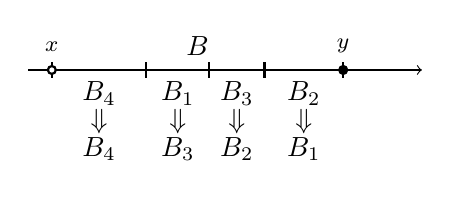
\begin{tikzpicture}
                \draw[->] (-1,0) -- (4,0);
                \begin{scope}[style = thick]
                    \draw (3,-0.1) -- (3,0.1);
                    \draw (2,-0.1) -- (2,0.1);
                    \draw (1.3,-0.1) -- (1.3,0.1);
                    \draw (0.5,-0.1) -- (0.5,0.1);
                    \draw (-0.7,-0.1) -- (-0.7,0.1);
                    \draw (3,0) -- (-0.7,0);
                \end{scope}
                \begin{scope}[every node/.append style = {font = \footnotesize}]
                    \node at (3,0.3) {$y$};
                    \node at (-0.7,0.3) {$x$};
                \end{scope}
                \node at (2.5,-0.3) {$B_2$};
                \node at (1.65,-0.3) {$B_3$};
                \node at (0.9,-0.3) {$B_1$};
                \node at (-0.1,-0.3) {$B_4$};
                \node at (2.5,-0.65) {$\Downarrow$};
                \node at (1.65,-0.65) {$\Downarrow$};
                \node at (0.9,-0.65) {$\Downarrow$};
                \node at (-0.1,-0.65) {$\Downarrow$};
                \node at (2.5,-1) {$B_1$};
                \node at (1.65,-1) {$B_2$};
                \node at (0.9,-1) {$B_3$};
                \node at (-0.1,-1) {$B_4$};
                \node at (1.15,0.3) {$B$};
                \begin{scope}[style = thick]
                    \draw[fill = black] (3,0) circle[radius = 0.05];
                    \draw[fill = white] (-0.7,0) circle[radius = 0.05];
                \end{scope}
            \end{tikzpicture}
        }
        \qquad
        \subfigure{
            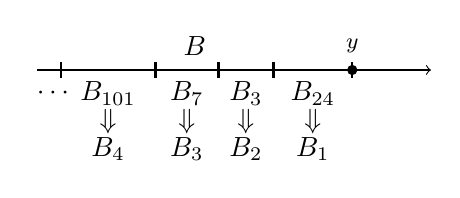
\begin{tikzpicture}
                \draw[->] (-1,0) -- (4,0);
                \begin{scope}[style = thick]
                    \draw (3,-0.1) -- (3,0.1);
                    \draw (2,-0.1) -- (2,0.1);
                    \draw (1.3,-0.1) -- (1.3,0.1);
                    \draw (0.5,-0.1) -- (0.5,0.1);
                    \draw (-0.7,-0.1) -- (-0.7,0.1);
                    \draw (3,0) -- (-1,0);
                    \draw[fill = black] (3,0) circle[radius = 0.05];
                \end{scope}
                \begin{scope}[every node/.append style = {font = \footnotesize}]
                    \node at (3,0.3) {$y$};
                \end{scope}
                \node at (2.5,-0.3) {$B_{24}$};
                \node at (1.65,-0.3) {$B_3$};
                \node at (0.9,-0.3) {$B_7$};
                \node at (-0.1,-0.3) {$B_{101}$};
                \node at (-0.8,-0.3) {$\cdots$};
                \node at (2.5,-0.65) {$\Downarrow$};
                \node at (1.65,-0.65) {$\Downarrow$};
                \node at (0.9,-0.65) {$\Downarrow$};
                \node at (-0.1,-0.65) {$\Downarrow$};
                \node at (2.5,-1) {$B_1$};
                \node at (1.65,-1) {$B_2$};
                \node at (0.9,-1) {$B_3$};
                \node at (-0.1,-1) {$B_4$};
                \node at (1,0.3) {$B$};
            \end{tikzpicture}
        }
        \vspace{-3em}
    \end{figure}
    \begin{figure}[!ht]
        \centering
        \subfigure{
            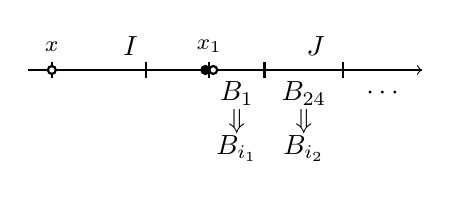
\begin{tikzpicture}
                \draw[->] (-1,0) -- (4,0);
                \begin{scope}[style = thick]
                    \draw (3,-0.1) -- (3,0.1);
                    \draw (2,-0.1) -- (2,0.1);
                    \draw (1.3,-0.1) -- (1.3,0.1);
                    \draw (0.5,-0.1) -- (0.5,0.1);
                    \draw (-0.7,-0.1) -- (-0.7,0.1);
                    \draw (4,0) -- (-0.7,0);
                    \draw[fill = white] (-0.7,0) circle[radius = 0.05];
                    \draw[fill = white] (1.35,0) circle[radius = 0.05];
                    \draw[fill = black] (1.25,0) circle[radius = 0.05];
                \end{scope}
                \begin{scope}[every node/.append style = {font = \footnotesize}]
                    \node at (-0.7,0.3) {$x$};
                    \node at (1.3,0.3) {$x_1$};
                \end{scope}
                \node at (2.5,-0.3) {$B_{24}$};
                \node at (1.65,-0.3) {$B_1$};
                \node at (3.5,-0.3) {$\cdots$};
                \node at (2.5,-0.65) {$\Downarrow$};
                \node at (1.65,-0.65) {$\Downarrow$};
                \node at (2.5,-1) {$B_{i_2}$};
                \node at (1.65,-1) {$B_{i_1}$};
                \node at (2.65,0.3) {$J$};
                \node at (0.3,0.3) {$I$};
            \end{tikzpicture}
        }
        \qquad
        \subfigure{
            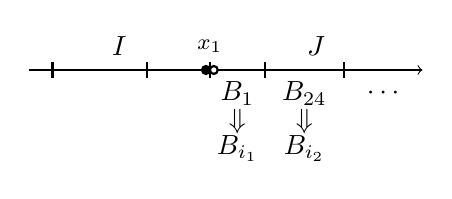
\begin{tikzpicture}
                \draw[->] (-1,0) -- (4,0);
                \begin{scope}[style = thick]
                    \draw (3,-0.1) -- (3,0.1);
                    \draw (2,-0.1) -- (2,0.1);
                    \draw (1.3,-0.1) -- (1.3,0.1);
                    \draw (0.5,-0.1) -- (0.5,0.1);
                    \draw (-0.7,-0.1) -- (-0.7,0.1);
                    \draw (4,0) -- (-1,0);
                    \draw[fill = white] (1.35,0) circle[radius = 0.05];
                    \draw[fill = black] (1.25,0) circle[radius = 0.05];
                \end{scope}
                \begin{scope}[every node/.append style = {font = \footnotesize}]
                    \node at (1.3,0.3) {$x_1$};
                \end{scope}
                \node at (2.5,-0.3) {$B_{24}$};
                \node at (1.65,-0.3) {$B_1$};
                \node at (3.5,-0.3) {$\cdots$};
                \node at (2.5,-0.65) {$\Downarrow$};
                \node at (1.65,-0.65) {$\Downarrow$};
                \node at (2.5,-1) {$B_{i_2}$};
                \node at (1.65,-1) {$B_{i_1}$};
                \node at (2.65,0.3) {$J$};
                \node at (0.15,0.3) {$I$};
            \end{tikzpicture}
        }
        \caption{명제 \ref{prop:lebesguePremeasure}의 증명에서 $n=1$인 경우 $B$의 형태로 가능한 네 가지 경우에 대한 $\{B_i\}$의 재배열 과정. 각각 $B=(x,\,y]$ (왼쪽 위), $B=(-\infty,\,y]$ (오른쪽 위), $B=(x,\,\infty)$ (왼쪽 아래), $B=(-\infty,\,\infty)$ (오른쪽 아래)인 경우를 나타낸다.}
    \end{figure}

    이제 일반적인 $n\in\mathbb{N}$의 경우를 생각하면 적당한 반열린구간 $I_1,\,\cdots,\,I_n\subseteq\mathbb{R}$에 대해 $B=\prod_{j=1}^nI_j$로 쓸 수 있다. 우선 $\{B_i\}$가 $B$의 `\texttt{regular tilling}'을 이루는 경우를 먼저 생각해보자. 여기서 \texttt{regular tilling}을 이룬다고 함은 $\{B_i\}$가 $B$를 딱 맞아떨어지게 채워넣는 경우를 이르는 것으로, 보다 엄밀하게, 각 $j\leq n$에 대해 $I_j$를 가산개의 반열린구간 $I_{j1},\,I_{j2},\,\cdots$로 분할할 수 있어서 이러한 분할들이 이루는 \texttt{semi-open box}들이 모두 정확히 하나의 $B_i$와 일치하는 경우를 이른다.

    \begin{figure}[!ht]
        \centering
        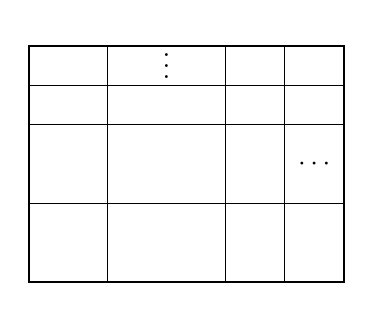
\begin{tikzpicture}
            \draw[style = thick] (0,0) -- (4,0) -- (4,3) -- (0,3) -- cycle;
            \draw (0,1) -- (4,1);
            \draw (0,2) -- (4,2);
            \draw (0,2.5) -- (4,2.5);
            \draw (1,0) -- (1,3);
            \draw (2.5,0) -- (2.5,3);
            \draw (3.25,0) -- (3.25,3);
            \node at (1.75,2.85) {$\vdots$};
            \node at (3.625,1.5) {$\cdots$};
        \end{tikzpicture}
    \end{figure}
    
    \begin{figure}[!ht]
        \centering
        \subfigure{
            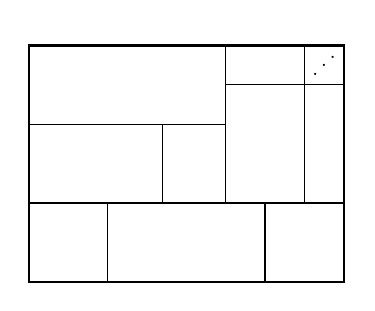
\begin{tikzpicture}
                \draw[style = thick] (0,0) -- (4,0) -- (4,3) -- (0,3) -- cycle;
                \draw (0,1) -- (4,1);
                \draw (0,2) -- (2.5,2);
                \draw (1,0) -- (1,1);
                \draw (3,0) -- (3,1);
                \draw (2.5,1) -- (2.5,3);
                \draw (1.7,1) -- (1.7,2);
                \draw (3.5,1) -- (3.5,3);
                \draw (2.5,2.5) -- (4,2.5);
                \node at (3.75,2.85) {\reflectbox{\scriptsize$\ddots$}};
            \end{tikzpicture}
        }
        \qquad
        \subfigure{
            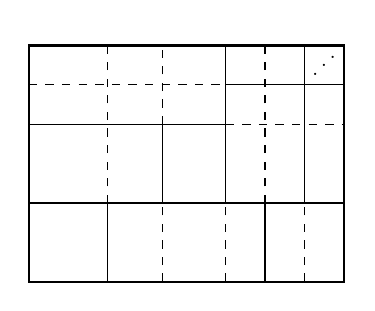
\begin{tikzpicture}
                \draw[style = thick] (0,0) -- (4,0) -- (4,3) -- (0,3) -- cycle;
                \draw (0,1) -- (4,1);
                \draw (0,2) -- (2.5,2);
                \draw (1,0) -- (1,1);
                \draw (3,0) -- (3,1);
                \draw (2.5,1) -- (2.5,3);
                \draw (1.7,1) -- (1.7,2);
                \draw (3.5,1) -- (3.5,3);
                \draw (2.5,2.5) -- (4,2.5);
                \node at (3.75,2.85) {\reflectbox{\scriptsize$\ddots$}};
                \begin{scope}[style = dashed]
                    \draw (1.7,0) -- (1.7,1);
                    \draw (2.5,0) -- (2.5,1);
                    \draw (1,1) -- (1,3);
                    \draw (3,1) -- (3,3);
                    \draw (2.5,2) -- (4,2);
                    \draw (1.7,2) -- (1.7,3);
                    \draw (3.5,0) -- (3.5,1);
                    \draw (0,2.5) -- (2.5,2.5);
                \end{scope}
            \end{tikzpicture}
        }
        \caption{명제 \ref{prop:lebesguePremeasure}의 증명에서 집합열 $\{B_i\}$가 $B$의 \texttt{regular tilling}을 이루는 경우.(위) 집합열 $\{B_i\}$가 \texttt{regular tilling}을 이루지 않는 경우에 이의 각 면을 연장하여 \texttt{regular tilling}을 이루도록 하는 과정.(아래)}
    \end{figure}

    이 경우, 만약 $B$가 유계라면 곧 모든 $I_1,\,\cdots,\,I_n$도 유계이고, 앞선 결과로부터
    \begin{align*}
        \rho_n(B)&=\prod_{j=1}^n\rho_1(I_j)\\
        &=\prod_{j=1}^n\sum_{k=1}^{l_j}\rho_1(I_{jk})\\
        &=\sum_{k_1=1}^{l_1}\cdots\sum_{k_n=1}^{l_n}\prod_{j=1}^n\rho_1(I_{j{k_j}})\\
        &=\sum_{k_1=1}^{l_1}\cdots\sum_{k_n=1}^{l_n}\rho_n\bigg(\prod_{j=1}^nI_{j{k_j}}\bigg)\\
        &=\sum_{i=1}^\infty\rho_n(B_i)
    \end{align*}
    임을 안다. (여기서 $l_1,\,\cdots,\,l_n$은 유한할 수도 있고, $\infty$일 수도 있다.) 만약 $B$가 유계가 아니라면 \texttt{WLOG}, $I_1$이 유계가 아니라 해도 되고, 이번에도 앞선 결과로부터
    \begin{align*}
        \sum_{k=1}^{l_1}\rho_n\bigg(I_{1k}\times\prod_{j=2}^nI_{j1}\bigg)&=\bigg[\sum_{k=1}^{l_1}\rho_1(I_{1k})\bigg]\prod_{j=2}^n\rho_1(I_{j1})\\
        &=\rho_1(I_1)\prod_{j=2}^n\rho_1(I_{j1})\\
        &=\infty
    \end{align*}
    가 되어 $\sum_{i=1}^\infty\rho_n(B_i)\geq\sum_{k=1}^{l_1}\rho_n(I_{1k}\times\prod_{j=2}^nI_{j1})=\infty=\rho(B)$를 얻는다. 다음으로, $\{B_i\}$가 $B$의 \texttt{regular tilling}을 이루지 않는 경우를 생각해보자. 이 경우에는 각 $B_i$의 면을 연장하여 $B$를 가산개의 \texttt{semi-open box} $C_1,\,C_2,\,\cdots$로 분할할 수 있으며 \texttt{WLOG}, 필요하다면 공집합을 추가하여 이가 집합열 $\{C_j\}$을 이룬다고 해도 된다. (공집합은 $\emptyset = \prod_{j=1}^n(0,\,0]$에서 명백히 \texttt{semi-open box}이다.) 그렇다면 모든 $j\in\mathbb{N}$에 대해 $C_j\subseteq B_i$인 $i\in\mathbb{N}$가 유일하게 존재하며, $\{C_j\}$는 모든 $B_i$와 $B$의 \texttt{regular tilling}을 이룬다. 따라서 $\rho_n(B)=\sum_{j=1}^\infty\rho_n(C_j)=\sum_{i=1}^\infty\sum_{j:C_j\subseteq B_i}\rho_n(C_j)=\sum_{i=1}^\infty\rho_n(B_i)$이고, 곧 어떠한 경우에도 $\rho_n$이 $\sigma$-가법성을 가짐을 알 수 있으므로 증명이 끝난다.
\end{proof}

이와 같이 정의된 $\mathcal{S}_n$ 위의 \texttt{premeasure} $\rho_n$이 우리의 출발점이다. 여기에 정리 \ref{thm:semiAlgebraExtension}를 사용하면 $\mathcal{S}_n$ 위의 \texttt{premeasure} $\rho_n$을 $A(\mathcal{S}_n)$에서의 \texttt{premeasure}로 유일하게 확장할 수 있고, 이제부터는 표기를 남용하여 이러한 유일한 확장을 $\rho_n$이라 쓰도록 하겠다. 이러한 확장 $\rho_n$이 $\sigma$-유한함은 쉽게 확인할 수 있다.

\begin{proposition}
    대수 $A(\mathcal{S}_n)$ 위의 \texttt{premeasure} $\rho_n$은 $\sigma$-유한하다.
\end{proposition}

\begin{proof}
    $\bigsqcup_{x\in\mathbb{Z}^n}(x,\,x+\ind]=\mathbb{R}^n$이고 모든 $x\in\mathbb{Z}^n$에 대해 $\rho_n((x,\,x+\ind])=1$이므로 이는 자명하다.
\end{proof}

마지막 단계로, \texttt{premeasure} $\rho_n$으로부터 유도되는 $\mathcal{P}(\mathbb{R}^n)$ 위의 외측도 $\rho_n^*$을 생각하고 $\mathcal{M}_n$을 모든 $\rho_n^*$-가측집합의 모임이라 하자. 그렇다면 \texttt{Carath\'eodory}의 확장정리와 정리 \ref{thm:CaratheodoryUnique}로부터 $A(\mathcal{S}_n)$위의 \texttt{premeasure} $\rho_n$을 $\mathcal{M}_n$ 위의 측도로 유일하게 확장할 수 있고, 이가 우리가 그토록 원하던 \texttt{Lebesgue} 측도이다.

\begin{definition}
    위에서와 같이 확장된 $A(\mathcal{S}_n)$위의 \texttt{premeasure} $\rho_n$에 대해 이의 \texttt{Carath\'eodory} 확장을 \textbf{\texttt{Lebesgue} 측도(- \texttt{measure})}라 하고 $\lambda_n$으로 쓴다. 또한, 이때 $\lambda_n$의 정의역인 모든 $\rho_n^*$-가측집합들의 모임을 $\mathcal{M}_n$으로 쓰고, \texttt{triple} $(\mathbb{R}^n,\,\mathcal{M}_n,\,\lambda_n)$을 \textbf{\texttt{Lebesgue} 측도공간(- \texttt{measure space})}이라 한다.
\end{definition}

보통 특별히 정하지 않는 이상 $\mathbb{R}^n$에는 \texttt{Lebesgue} 측도 $\lambda_n$이 주어진 것으로 보고, 이는 이 책에서도 마찬가지이다.

이로써 우리의 첫 번째 \texttt{Lebesgue} 측도의 구성이 일단락되었다. 그러나 아직 몇몇 답하기 어려운 질문들이 남아있다. 그 중 하나로, $\sigma$-대수 $\mathcal{M}_n$을 한 번 살펴보자. 과연 이는 어떤 집합들로 이루어져 있을까? \texttt{Lebesgue} 측도의 구성 과정에서 $A(\mathcal{S}_n)$의 구조까지는 쉽게 상상이 가지만 \texttt{Carath\'eodory}의 확장정리의 다소 현란한 확장 방식 덕에 $\mathcal{M}_n$의 구조는 쉽게 손에 잡히지 않는다. 우리가 앞으로 기본적인 측도공간으로 삼을 \texttt{Lebesgue} 측도공간의 구조를 모른다는 것은 그다지 유쾌한 일이 아니며, 이는 곧 \texttt{Lebesgue} 측도의 구성은 마쳤지만 $\mathbb{R}^n$의 부분집합 중에서 \texttt{Lebesgue} 측도로써 잴 수 있는 집합과 그렇지 않은 집합을 구별할 수 있는 기준은 여전히 모호하다는 뜻이다.

사실, $\mathcal{M}_n$은 생각보다 굉장히 큰 $\sigma$-대수이다. 우리가 상식적인 선에서 생각해 낼 수 있는 거의 대부분의 집합, 예컨대 (표준 위상에 대해) 열린집합, 닫힌집합, 가산 집합, \texttt{box}나 \texttt{\texttt{ball}}, 혹은 $\mathbb{N}^n,\,\mathbb{Z}^n,\,\mathbb{Q}^n$ 따위의 집합들은 $\mathcal{M}_n$의 극히 일부분을 차지할 뿐이다. 집합족 $\mathcal{M}_n$의 대부분은 정말 상상조차 하기 힘든 괴상한 집합들로 이루어져 있어 $\mathcal{M}_n$은 그다지 경제적인 $\sigma$-대수는 못된다.\footnotemark\label{note:lebesgueCardinal} 어쩌면 1절에서 지적한 것과 같이 측도를 부여할 집합으로 너무 많은 것들을 택한 것일 수도 있다. 그럼에도 불구하고 (이후에 자세히 보겠지만) 이 거대한 $\mathcal{M}_n$ 위에서 \texttt{Lebesgue} 측도는 놀라우리만치 바람직한 성질들을 가지기에 단순히 $\mathcal{M}_n$이 너무 크다는 이유로 힘들게 구성해낸 \texttt{Lebesgue} 측도공간을 포기하기는 뭔가 아쉽다. 이 상황을 타개할 현명한 해결책은 바로 $\mathcal{M}_n$ 중에서 이상한 집합들을 모두 걷어내고 `실용적'인 집합들만 골라 $\mathcal{M}_n$ 보다 작은 $\sigma$-대수를 적당히 만든 다음 \texttt{Lebesgue} 측도를 그 $\sigma$-대수로 제한시키는 것이다. 이렇게 하면 이 새로운 측도공간은 \texttt{Lebesgue} 측도공간의 바람직한 성질들을 그대로 상속받으면서 훨씬 더 가볍고 경제적인 $\sigma$-대수로 구성되어 그 구조도 선명히 파악할 수 있을 것이다. 언듯 보기에 이 과정 또한 \texttt{Lebesgue} 측도의 구성 못지않게 꽤나 복잡할 것 같지만, 사실 $\mathbb{R}^n$의 열린집합을 모으는 것만으로 충분하다.

\begin{definition}
    집합족 $\mathcal{U}$를 $\mathbb{R}^n$의 모든 열린집합의 모임이라 하자. 이때 $\mathcal{U}$가 생성하는 $\sigma$-대수를 \textbf{\texttt{Borel} $\sigma$-대수(- $\sigma$-\texttt{algebra})}라 하고 $\mathcal{B}_n$으로 쓴다. 나아가, $\mathcal{B}_n$에 속하는 임의의 집합을 \textbf{\texttt{Borel} 집합(- \texttt{set})}이라 한다.
\end{definition}

\begin{proposition}
    집합 $\mathbb{R}^n$의 열린집합이나 닫힌집합에 교집합, 합집합, 여집합, 차집합 혹은 이들을 가산번 조합하여 정의한 연산을 취하여 얻는 집합은 \texttt{Borel}이다.
\end{proposition}

\begin{proof}
    임의의 닫힌집합 $F\subseteq\mathbb{R}^n$에 대해 그 정의로부터 $F^c$가 열린집합이므로 $F$는 \texttt{Borel}이다. 이제 $\mathcal{B}_n$이 $\sigma$-대수로서 교집합, 합집합, 여집합, 차집합 그리고 이들을 가산번 조합한 연산에 대해 모두 닫혀있음을 생각하면 이 명제는 자명하다.
\end{proof}

단순히 $\mathbb{R}^n$의 열린집합을 모아 이들로 $\sigma$-대수를 생성한 것 뿐인데 우리가 상식적으로 떠올릴 수 있는 거의 대부분이 집합이 \texttt{Borel} $\sigma$-대수에 속한다는 사실을 알 수 있다. 따라서 $\mathcal{B}_n\subseteq\mathcal{M}_n$만 성립한다면 모든 문제가 해결된다. 이는 $\mathcal{B}_n$의 생성자를 조금 더 조사해보면 바로 알 수 있다.

\begin{theorem}\label{thm:BorelGen1}
    집합족 $\mathcal{C}$를 $\mathbb{R}^n$의 모든 유계인 열린 \texttt{box}의 모임이라 하면 이는 $\mathcal{B}_n$의 생성자이다.
\end{theorem}

\begin{proof}
    집합족 $\mathcal{U}$를 $\mathbb{R}^n$의 모든 열린집합의 모임이라 하면 $\mathcal{C}\subseteq\mathcal{U}$이므로 $\sigma(\mathcal{C})\subseteq\mathcal{B}_n$임은 분명하다. 이제 $\mathbb{R}^n$의 모든 열린집합은 유계인 열린 \texttt{box}의 가산 합집합으로 표현된다는 점\footnotemark\label{note:countableOpenBox}을 생각해보면 $\mathcal{U}\subseteq\sigma(\mathcal{C})$이고, 곧 $\mathcal{B}_n\subseteq\sigma(\mathcal{C})$가 되어 증명이 끝난다.
\end{proof}

\begin{theorem}\label{thm:BorelGen2}
    집합족 $\mathcal{S}_n$은 $\mathcal{B}_n$의 생성자이다.
\end{theorem}

\begin{proof}
    간결한 논의를 위해 $n=1$인 경우만 생각하자. (일반적인 경우에도 이와 비슷하게 보일 수 있다.) 또한 $\mathcal{C}$를 $\mathbb{R}$의 모든 유계인 열린 \texttt{box}의 모임이라 하자. 그렇다면 임의의 $B\in\mathcal{C}$에 대해 적당한 $x,\,y\in\mathbb{R}$가 존재하여 $B=(x,\,y)$이고, $(x,\,y)=\bigcup_{i=1}^\infty(x,\,y-1/i]$에서 $\mathcal{C}\subseteq\sigma(\mathcal{S}_1)$이므로 곧 $\sigma(\mathcal{C})\subseteq\sigma(\mathcal{S}_1)$이다. 이제 역의 포함관계를 보이기 위해 임의의 $I\in\mathcal{S}_1$를 택하면 정의로부터 $I$는 적당한 $x,\,y\in\mathbb{R}$에 대해 $(x,\,y],\,(-\infty,\,y],\,(x,\,\infty),\,(-\infty,\,\infty)$ 중 하나의 형태로 나타낼 수 있다. 이번에도 간결한 논의를 위해 첫 번째 경우만 생각해보자. (나머지 경우들도 비슷하게 따져보면 동일한 결론을 얻는다.) $I=(x,\,y]$라 하면 $I=(x,\,\infty)\setminus(y,\,\infty)=\bigcup_{i=1}^\infty(x,\,x+i)\setminus\bigcup_{i=1}^\infty(y,\,y+i)$이므로 $I\in\sigma(\mathcal{C})$이고, 곧 $\mathcal{S}_1\subseteq\sigma(\mathcal{C})$가 되어 $\sigma(\mathcal{S}_1)\subseteq\sigma(\mathcal{C})$임을 안다. 이제 정리 \ref{thm:BorelGen1}로부터 $\sigma(\mathcal{S}_1)=\mathcal{B}_1$이 되어 정리가 증명된다.
\end{proof}

여기서 $\mathcal{M}_n$이 $\mathcal{S}_n$을 포함한다는 사실을 떠올린다면, $\mathcal{B}_n\subseteq\mathcal{M}_n$임은 당연하다.\footnotemark 이제 우리는 다음을 정의할 수 있다.

\begin{definition}
    \texttt{Lebesgue} 측도 $\lambda_n$에 대해 이의 $\mathcal{B}_n$으로의 제한 $\lambda_n\vert_{\mathcal{B}_n}$을 \textbf{\texttt{Borel} 측도(- \texttt{measure})}라 하고 $\mu_n$으로 쓴다. 나아가, \texttt{triple} $(\mathbb{R}^n,\,\mathcal{B}_n,\,\mu_n)$을 \textbf{\texttt{Borel} 측도공간(- \texttt{measure space})}이라 한다.
\end{definition}

나중에 사용하기 위해 $\mathcal{B}_n$의 생성자를 하나만 더 소개한다.

\begin{theorem}\label{thm:BorelGen3}
    집합족 $\mathcal{C}$를 어떤 $x\in\mathbb{R}^n$에 대해 $(-\infty,\,x]$로 표현되는 $\mathbb{R}^n$의 모든 부분집합의 모임이라 하면 이는 $\mathcal{B}_n$의 생성자이다.
\end{theorem}

\begin{proof}
    간결한 논의를 위해 $n=1$인 경우만 생각하자. (일반적인 경우에도 이와 비슷하게 보일 수 있다.) 우선, $\mathcal{C}\subseteq\mathcal{S}_1$이므로 $\sigma(\mathcal{C})\subseteq\sigma(\mathcal{S}_1)$임은 분명하다. 이제 역의 포함관계를 보이기 위해 임의의 $I\in\mathcal{S}_1$를 택하면 정의로부터 $I$는 적당한 $x,\,y\in\mathbb{R}$에 대해 $(x,\,y],\,(-\infty,\,y],\,(x,\,\infty),\,(-\infty,\,\infty)$ 중 하나의 형태로 나타낼 수 있다. 이번에도 간결한 논의를 위해 첫 번째 경우만 생각해보자.  (나머지 경우들도 비슷하게 따져보면 동일한 결론을 얻는다.) $I=(x,\,y]$라 하면 $I=(-\infty,\,y]\setminus(-\infty,\,x]$이므로 $I\in\sigma(\mathcal{C})$이고, 곧 $\mathcal{S}_1\subseteq\sigma(\mathcal{C})$가 되어 $\sigma(\mathcal{S}_1)\subseteq\sigma(\mathcal{C})$임을 안다. 이제 정리 \ref{thm:BorelGen2}로부터 $\sigma(\mathcal{C})=\mathcal{B}_1$이 되어 정리가 증명된다.
\end{proof}

\texttt{Lebesgue} 측도의 중요한 성질 몇 가지를 알아보자.

\begin{theorem}\label{thm:boundedMeasure}
    임의의 유계인 $A\in\mathcal{M}_n$에 대해 $\lambda_n(A)<\infty$이다.
\end{theorem}

\begin{proof}
    집합 $A$가 유계이므로 적당한 $M>0$에 대해 $A\subseteq(-M,\,M]^n$이고, 곧 $\lambda_n(A)\leq\lambda_n((-M,\,M]^n)=(2M)^n<\infty$에서 이 정리는 자명하다.
\end{proof}

\begin{theorem}\label{thm:LebesgueRegular}
    \texttt{Lebesgue} 측도 $\lambda_n$는 \texttt{regular}하다. 즉, 다음 두 가지 성질이 성립한다.
    \begin{enumerate}
        \item 임의의 $A\in\mathcal{M}_n$에 대해 $\lambda_n(A)=\inf\{\lambda_n(U)\in\overline{\mathbb{R}}^+_0:A\subseteq U\subseteq\mathbb{R}^n,\,U\textrm{는 열린집합}\}$이다.
        \item 임의의 $A\in\mathcal{M}_n$에 대해 $\lambda_n(A)=\sup\{\lambda_n(K)\in\overline{\mathbb{R}}^+_0:K\subseteq A,\,K\textrm{는 \texttt{compact} 집합}\}$이다.
    \end{enumerate}
\end{theorem}

\begin{proof}
    i. 만약 $\lambda_n(A)=\infty$이면 어떠한 열린집합 $U\supseteq A$에 대해서도 $\lambda_n(U)\geq\lambda_n(A)=\infty$가 되어 정리가 자명하므로 $\lambda_n(A)<\infty$라 가정하자. 한편, 임의의 열린집합 $U\supseteq A$에 대해 $\lambda_n(U)\geq\lambda_n(A)$임이 분명하므로 임의의 $\epsilon>0$을 택하고 적당한 열린집합 $U\supseteq A$가 존재하여 $\lambda_n(U)<\lambda_n(A)+\epsilon$임을 보이면 충분하다. 이를 위해, $\lambda_n(A)$의 정의가 $\lambda_n(A)=\inf\{\sum_{i=1}^\infty\rho_n(A_i)\in\overline{\mathbb{R}}^+_0:\{A_i\}\textrm{는 $A(\mathcal{S}_n)$에 속하는 $A$의 가산 덮개이다.}\}$라는 점을 상기한다면 $A(\mathcal{S}_n)$에 속하는 적당한 $A$의 가산 덮개 $\{A_i\}$가 존재하여 \texttt{WLOG}, 필요하다면 공집합을 추가하여 이가 집합열을 이룬다고 하고 $\sum_{i=1}^\infty\rho_n(A_i)<\lambda_n(A)+\epsilon$이다. 한편, 정리 \ref{thm:genAlgebra}로부터 각 $i\in\mathbb{N}$에 대해 적당한 서로소인 $B_{i1},\,\cdots,\,B_{ik_i}\in\mathcal{S}_n$이 존재하여 $A_i=\bigsqcup_{j=1}^{k_i}B_{ij}$이고, 따라서 \texttt{WLOG}, 필요하다면 $A_i$를 $B_{i1},\,\cdots,\,B_{ik_i}$로 바꾸어 $\{A_i\}$가 처음부터 $\mathcal{S}_n$에 속한다고 해도 된다. 또한, $\lambda_n(A)<\infty$이므로 각 $A_i$도 유계이고 \texttt{WLOG}, 필요하다면 각 $A_i$를 조금씩 크게 하여 $A\subseteq\bigcup_{i=1}^\infty A_i^\circ:=U$라 해도 된다.\footnotemark 그렇다면 $U$가 열려있으므로 이는 가측이고, 곧 $\lambda_n(U)\leq\lambda_n(\bigcup_{i=1}^\infty A_i)\leq\sum_{i=1}^\infty\rho_n(A_i)\leq\lambda_n(A)+\epsilon$이 되어 증명이 끝난다.

    ii. 먼저 $A$가 유계인 경우를 생각하면 적당한 $r>0$에 대해 $A\subseteq B(r)$이다. 한편, 임의의 \texttt{compact}한 $K\subseteq A$에 대해 $\lambda_n(K)\leq\lambda_n(A)$이므로 임의의 $\epsilon>0$을 택하고 적당한 \texttt{compact} 집합 $K\subseteq  A$가 존재하여 $\lambda_n(K)>\lambda_n(A)-\epsilon$임을 보이면 충분하다. 이를 위해 앞서 보인 i을 이용하면 적당한 열린집합 $U\supseteq\overline{B(r)}\setminus A$가 존재하여 $\lambda_n(U)<\lambda(\overline{B(r)}\setminus A)+\epsilon$이다. 여기서 $K=\overline{B(r)}\setminus U$라 하면 이는 \texttt{compact}하고 $\overline{B(r)}\subseteq U\sqcup K$에서 $\lambda_n(U)+\lambda_n(K)=\lambda_n(U\sqcup K)\geq\lambda_n(\overline{B(r)})$인데, 이는 곧 $\lambda_n(K)\geq\lambda_n(\overline{B(r)})-\lambda_n(U)>\lambda_n(\overline{B(r)})-\lambda_n(\overline{B(r)}\setminus A)-\epsilon=\lambda_n(A)-\epsilon$임을 뜻하므로 이 경우에 대해서는 증명이 끝난다. 이제 일반적인 $A$에 대해 유계인 집합열 $\{A\cap B(i)\}_i$를 생각하면 $A\cap B(i)\uparrow A$이고 따라서 앞선 결론으로부터
    \begin{align*}
        \lambda_n(A)&=\lim_{i\to\infty}\lambda_n(A\cap B(i))\\
        &=\sup_{r>0}\lambda_n(A\cap B(r))\\
        &=\sup_{r>0}\sup\{\lambda_n(K)\in\overline{\mathbb{R}}^+_0:K\subseteq A\cap B(i),\,K\textrm{는 \texttt{compact} 집합}\}\\
        &=\sup\{\lambda_n(K)\in\overline{\mathbb{R}}^+_0:K\subseteq A,\,K\textrm{는 \texttt{compact} 집합}\}
    \end{align*}
    이 성립하여 일반적인 경우에 대해서도 증명이 끝난다.
\end{proof}

\begin{figure}[!ht]
    \centering
    \subfigure{
        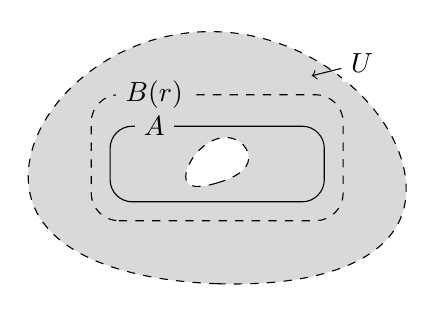
\begin{tikzpicture}[scale = 0.8]
            \begin{scope}[style = dashed]
                \draw[fill = gray!30!white] plot[smooth cycle, tension = 1] coordinates{(-1,0.7) (2,-1) (5,0.5) (2,3)};
                \draw[rounded corners = 10pt] (0,0) -- (4,0) -- (4,2) -- (0, 2) -- cycle;
                \draw[fill = white] plot[smooth cycle, tension = 1] coordinates{(1.5,0.7) (2,0.6) (2.5,1) (2,1.3)};
            \end{scope}
            \draw[rounded corners = 8pt] (0.3,0.3) -- (3.7,0.3) -- (3.7,1.5) -- (0.3,1.5) -- cycle;
            \node[fill = gray!30!white] at (1,2) {$B(r)$};
            \node[fill = gray!30!white] at (1,1.5) {$A$};
            \node[fill = white] (U) at (4.3,2.5) {$U$};
            \draw[->] (U) -- (3.5,2.3);
        \end{tikzpicture}
    }
    \qquad
    \subfigure{
        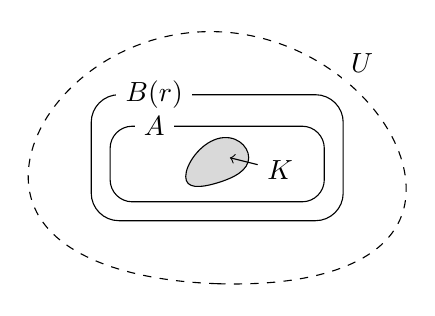
\begin{tikzpicture}[scale = 0.8]
            \draw[rounded corners = 10pt] (0,0) -- (4,0) -- (4,2) -- (0, 2) -- cycle;
            \draw[rounded corners = 8pt] (0.3,0.3) -- (3.7,0.3) -- (3.7,1.5) -- (0.3,1.5) -- cycle;
            \draw[style = dashed] plot[smooth cycle, tension = 1] coordinates{(-1,0.7) (2,-1) (5,0.5) (2,3)};
            \draw[fill = gray!30!white] plot[smooth cycle, tension = 1] coordinates{(1.5,0.7) (2,0.6) (2.5,1) (2,1.3)};
            \node[fill = white] at (1,2) {$B(r)$};
            \node[fill = white] at (1,1.5) {$A$};
            \node[fill = white] at (4.3,2.5) {$U$};
            \node (K) at (3,0.8) {$K$};
            \draw[->] (K) -- (2.2,1);
        \end{tikzpicture}
    }
    \caption{정리 \ref{thm:LebesgueRegular}의 ii의 증명에서 집합 $U$ (왼쪽)와 집합 $K$ (오른쪽).}
\end{figure}

\begin{theorem}\label{thm:lebesgueTranslation}
    \texttt{Lebesgue} 측도 $\lambda_n$는 이동 불변성을 갖는다. 즉, 임의의 $A\in\mathcal{M}_n$와 임의의 $x\in\mathbb{R}^n$에 대해 $A+x\in\mathcal{M}_n$이고 $\lambda_n(A+x)=\lambda_n(A)$이다.
\end{theorem}

\begin{proof}
    만약 $A\in A(\mathcal{S}_n)$이라면 이 정리는 자명하다. 이제 임의의 $B\subseteq\mathbb{R}^n$에 대해 $\{B_i\}$를 $A(\mathcal{S}_n)$에 속하는 $B$의 가산 덮개라 하면 $\{B_i+x\}$는 $A(\mathcal{S}_n)$에 속하는 $B+x$의 가산 덮개가 되고, 이의 역도 성립하므로 $\rho_n^*(B)=\rho_n^*(B+x)$임을 안다. 이러한 결론이 임의의 $B\subseteq\mathbb{R}^n$에 대해 성립한다는 사실을 상기한다면, $A+x$가 가측이라는 사실만 보이는 것으로 충분함을 알 수 있다. 이를 위해 임의의 $S\subseteq\mathbb{R}^n$를 생각하면 $A$가 가측이라는 사실과 앞선 결과로부터 $\rho_n^*(S\cap(A+x))+\rho_n^*(S\cap(A+x)^c)=\rho_n^*((S-x)\cap A)+\rho_n^*((S-x)\cap A^c)=\rho_n^*(S-x)=\rho_n^*(S)$가 되어 $A+x$가 가측임을 알고, 곧 증명이 끝난다.
\end{proof}

마지막으로 $\mathcal{B}_n$에 관한 놀라운 결과 하나를 소개하는 것으로 이번 절을 마치도록 하자. 이러한 결과는 $\mathcal{B}_n$이 $\mathcal{M}_n$보다 작은 $\sigma$-대수로 그 구조가 비교적 명확하다는 점에 크게 기인한다. ($\mathcal{B}_n$의 생성자는 서너개 알고 있는 반면, $\mathcal{M}_n$의 생성자나 구조는 여전히 오리무중이다.)

\begin{definition}
    집합 $A\subseteq\mathbb{R}^n$에서 정의된 함수 $f:A\to\mathbb{R}$와 유계인 \texttt{semi-open box} $B\subseteq A$에 대해 $B$가 적당한 $x,\,y\in\mathbb{R}^n$에 대해 $B=(x,\,y]$와 같이 표현된다고 하자. 이때,
    \begin{equation*}
        \sum_{0\leq\alpha\leq1}(-1)^{|\alpha|}f(x_1^{1-\alpha_1}y_1^{\alpha_1},\,\cdots,\,x_n^{1-\alpha_n}y_n^{\alpha_n})
    \end{equation*}
     를 $f$의 \textbf{$B$에서의 \texttt{difference}}라 하고 $\Delta_Bf$로 쓴다.
\end{definition}

\begin{theorem}\label{thm:distributionProp}
    유한 측도공간 $(\mathbb{R}^n,\,\mathcal{B}_n,\,\mu)$에 대해 함수 $F_\mu:\mathbb{R}^n\to\mathbb{R}$를 $F_\mu:x\mapsto\mu((-\infty,\,x])$로 정의하면 다음이 성립한다.

    \begin{enumerate}
        \item 함수 $F_\mu$는 $\mu(\mathbb{R}^n)$에 의해 위로 유계이다.
        \item 임의의 유계인 \texttt{semi-open box} $B\subseteq\mathbb{R}^n$에 대해 $\Delta_BF_\mu=\mu(B)\geq0$이다.
        \item 함수 $F_\mu$는 각 변수에 대해 증가한다.
        \item 함수 $F_\mu$는 오른쪽 연속이다.
        \item 함수 $F_\mu$는 각 변수에 대해 오른쪽 연속이다.
        \item 각 $i\leq n$에 대해 $\lim_{x_i\to-\infty}F_\mu(x)=0$이다.
        \item $\lim_{x_1,\,\cdots,\,x_n\to\infty}F_\mu(x)=\mu(\mathbb{R}^n)$.
    \end{enumerate}
\end{theorem}

\begin{proof}
    i. 임의의 $x\in\mathbb{R}^n$에 대해 $F_\mu(x)=\mu((-\infty,\,x])\leq\mu(\mathbb{R}^n)<\infty$이므로 이는 자명하다.

    ii. 간결한 논의를 위해 $n=2$인 경우만 생각하도록 하자. ($n=1$인 경우를 포함한 일반적인 경우도 이와 비슷하게 보일 수 있다.) 그렇다면 적당한 $x,\,y\in\mathbb{R}^2$에 대해 $B=(x_1,\,y_1]\times(x_2,\,y_2]$로 쓸 수 있으므로
    \begin{align*}
        \Delta_BF_\mu&=F_\mu(y_1,\,y_2)-F_\mu(x_1,\,y_2)-F_\mu(y_1,\,x_2)+F_\mu(x_1,\,x_2)\\
        &=\mu((-\infty,\,y_1]\times(-\infty,\,y_2])-\mu((-\infty,\,x_1]\times(-\infty,\,y_2])\\
        &\qquad\qquad\qquad-\mu((-\infty,\,y_1]\times(-\infty,\,x_2]+\mu((-\infty,\,x_1]\times(-\infty,\,x_2])\\
        &=\mu((-\infty,\,y_1]\times(-\infty,\,y_2]\setminus(-\infty,\,x_1]\times(-\infty,\,y_2])\\
        &\qquad\qquad\qquad-\mu((-\infty,\,y_1]\times(-\infty,\,x_2]\setminus(-\infty,\,x_1]\times(-\infty,\,x_2])\\
        &=\mu((x_1,\,y_1]\times(-\infty,\,y_2])-\mu((x_1,\,y_1]\times(-\infty,\,x_2])\\
        &=\mu((x_1,\,y_1]\times(-\infty,\,y_2]\setminus(x_1,\,y_1]\times(-\infty,\,x_2])\\
        &=\mu((x_1,\,y_1]\times(x_2,\,y_2])\\
        &=\mu(B)
    \end{align*}
    가 성립한다.

    iii. 간결한 논의를 위해 $F_\mu$가 첫 번째 변수에 대해 증가한다는 것만 보이자. (다른 변수에 대해서도 이와 비슷하게 보일 수 있다.) 이제 임의의 $x\in\mathbb{R}^n$와 임의의 $h\geq0$에 대해 $B=(-\infty,\,x],\,B'=(-\infty,\,x_1+h]\times\prod_{i=2}^{n}(-\infty,\,x_i]$라 하면 $F_\mu(x_1+h,\,\cdots)-F_\mu(x_1,\,\cdots)=\mu(B')-\mu(B)=\mu(B'\setminus B)\geq0$에서 증명이 끝난다.

    iv. 임의의 $x\in\mathbb{R}^n$를 택하여 $B=(-\infty,\,x]$라 하고, 집합열 $\{B_j\}$를 $B_j:=(-\infty,\,x+\ind/j]$로 두면 이는 $B$로 수렴하는 $\mathcal{S}_n$에 속하는 감소하는 집합열이므로 정리 \ref{thm:monoSeriesMeasure}의 ii에서 $\mu(B_j)\downarrow\mu(B)=F_\mu(x)$이고, 곧 임의의 $\epsilon>0$을 택하면 적당한 $j_0\in\mathbb{N}$가 존재하여 $\mu(B_{j_0})-F_\mu(x)<\epsilon$이다. 이제 $\delta=1/j_0$라 하면 $||x-y||<\delta$이고 $x\leq y$인 모든 $y\in\mathbb{R}^n$에 대해 $B\subseteq(-\infty,\,y]\subseteq B_{j_0}$에서 $F_\mu(x)=\mu(B)\leq F_\mu(y)=\mu((-\infty,\,y])\leq\mu(B_{j_0})<F_\mu(x)+\epsilon$이므로 곧 $|F_\mu(x)-F_\mu(y)|<\epsilon$이 되어 증명이 끝난다.

    v. 이는 iv로부터 자명하다.

    vi. 간결한 논의를 위해 $i=1$인 경우에 대해서만 보이도록 하자. (다른 경우에도 이와 비슷하게 보일 수 있다.) 이제 임의의 $x_2,\,\cdots,\,x_n\in\mathbb{R}$을 택하고 집합열 $\{B_j\}$를 $B_j:=(-\infty,\,-j]\times\prod_{i=2}^n(-\infty,\,x_i]$로 두면 이는 $\emptyset$으로 수렴하는 $\mathcal{S}_n$에 속하는 감소하는 집합열이므로 정리 \ref{thm:monoSeriesMeasure}의 ii에서 $\mu(B_j)\downarrow\mu(\emptyset)=0$이고, 곧 임의의 $\epsilon>0$을 택하면 적당한 $j_0\in\mathbb{N}$가 존재하여 $\mu(B_{j_0})<\epsilon$이다. 이제 $x_1\leq-j_0$인 임의의 $x_1\in\mathbb{R}$에 대해 $F_\mu(x_1,\,x_2,\,\cdots)\leq F_\mu(-j_0,\,x_2,\,\cdots)=\mu(B_{j_0})<\epsilon$이 되어 증명이 끝난다.

    vii. 집합열 $\{B_j\}$를 $B_j:=(-\infty,\,j]^n$으로 두면 이는 $\mathbb{R}^n$으로 수렴하는 $\mathcal{S}_n$에 속하는 증가하는 집합열이므로 정리 \ref{thm:monoSeriesMeasure}의 i에서 $\mu(B_j)\uparrow\mu(\mathbb{R}^n)$이고, 곧 임의의 $\epsilon>0$을 택하면 적당한 $j_0\in\mathbb{N}$가 존재하여 $\mu(\mathbb{R}^n)-\mu(B_{j_0})<\epsilon$이다. 이제 $x\geq j_0\ind$인 임의의 $x\in\mathbb{R}^n$에 대해 $B_{j_0}\subseteq(-\infty,\,x]$인데, 이와 i로부터 $\mu(\mathbb{R}^n)\geq F_\mu(x)=\mu((-\infty,\,x])\geq F_\mu(j_0\mathbf{1})=\mu(B_{j_0})>\mu(\mathbb{R}^n)-\epsilon$이므로 곧 $|F_\mu(x)-\mu(\mathbb{R}^n)|<\epsilon$이 되어 증명이 끝난다.
\end{proof}

\begin{theorem}\label{thm:finiteBorelSpecify}
    함수 $F:\mathbb{R}^n\to\mathbb{R}$에 대해 이가
    \begin{enumerate}
        \item 함수 $F$는 오른쪽 연속이고 각 변수에 대해 증가한다.
        \item 유계인  \texttt{semi-open box} $B\subseteq\mathbb{R}^n$에 대해 $\Delta_BF\geq0$이다.
        \item 각 $i\leq n$에 대해 $\lim_{x_i\to-\infty}F(x)=0$이다.
    \end{enumerate}
    를 만족하면 $F(x)=\mu((-\infty,\,x])$인 $\mathcal{B}_n$ 위의 측도 $\mu$가 유일하게 존재한다.
\end{theorem}

\begin{proof}
    집합족 $\mathcal{C}$를 어떤 $x\in\mathbb{R}^n$에 대해 $(-\infty,\,x]$로 표현되는 $\mathbb{R}^n$의 모든 부분집합의 모임이라 하자. 일단 정리의 조건을 만족하는 측도가 존재하기만 한다면 정리 \ref{thm:BorelGen3}로부터 $\mathcal{C}$가 $\mathcal{B}_n$의 생성자이고 이는 $\pi$-\texttt{system}이므로 정리 \ref{thm:measureUnique}에 의해 그 측도의 유일성은 자명하다. 따라서 존재성을 보이는 것으로 증명은 충분하다. 이를 위해 우리는 \texttt{Lebesgue} 측도를 구성할 때 썼던 방법을 비슷하게 사용하려고 한다. 우선 $\mathcal{S}_n$ 위의 적당한 \texttt{premeasure} $\rho$를 정의하고, 이에 정리 \ref{thm:semiAlgebraExtension}와 \texttt{Carath\'eodory}의 확장정리를 연달아 사용하여 $\rho$를 측도로 확장한 다음, 이를 다시 $\mathcal{B}_n$으로 제한하는 것이다. 또한, 간결한 논의를 위해 $n=2$인 경우만 생각하도록 하자. ($n=1$인 경우를 포함한 일반적인 경우에도 이와 비슷하게 보일 수 있다.)

    먼저 함수 $\rho:\mathcal{S}_2\to\overline{\mathbb{R}}^+_0$를
    \begin{equation*}
        \rho:B\mapsto
        \begin{dcases*}
            \Delta_BF&집합 $B$가 유계인 경우\\
            \infty&\texttt{ow.}
        \end{dcases*}
    \end{equation*}
    로 정의하면 $\rho(\emptyset)=0$임은 분명하다. 이제 이가 $\sigma$-가법성을 가진다는 것만 보이면 $\rho$가 \texttt{premeasure}임을 알 수 있는데, 이를 위해서는 보조정리 \ref{lem:Caratheodory}로부터 $\rho$가 가법성과 $\sigma$-반가법성을 가짐을 보이는 것으로 충분하다. 먼저 가법성을 보이기 위해 임의의 서로소인 $B_1,\,\cdots,\,B_l\in\mathcal{S}_2$를 생각하여 $B:=\bigsqcup_{i=1}^lB_i\in\mathcal{S}_2$이라 하면 적당한 반열린구간 $I_1,\,I_2\subseteq\mathbb{R}$에 대해 $B=I_1\times I_2$로 쓸 수 있다. 만약 $B_1,\,\cdots,\,B_l$ 중에서 유계가 아닌 집합이 있다면 당연히 $B$도 유계가 아니게 되어 이 경우에는 가법성이 자명하므로 $B_1,\,\cdots,\,B_l$이 모두 유계라 하자. 이제 경우를 나누어 $B_1,\,\cdots,\,B_l$이 $B$의 \texttt{regular tilling}을 이루는 경우를 먼저 생각해보자. (\texttt{Regular tilling}을 이룬다는 것의 의미는 명제 \ref{prop:lebesguePremeasure}의 증명을 참조하기 바란다.) 이 경우에는 $\sum_{i=1}^l\rho(B_i)=\sum_{i=1}^l\Delta_{B_i}F=\Delta_BF=\rho(B)$가 되어 $\rho$가 가법성을 가진다. 이제 $B_1,\,\cdots,\,B_l$이 \texttt{regular tilling}을 이루지 않는 경우를 생각해보자. 이 경우에는 $B_1,\,\cdots,\,B_l$들의 각 면을 연장하여 $B$를 유한개의 \texttt{semi-open box} $C_1,\,\cdots,\,C_{l'}$로 분할할 수 있으며, 모든 $k\leq l'$에 대해 $C_k\subseteq B_i$인 $i\leq l$가 유일하게 존재하여 $C_1,\,\cdots,\,C_{l'}$은 모든 $B_1,\,\cdots,\,B_l$과 $B$의 \texttt{regular tilling}을 이룬다. 따라서 앞선 결과로부터 $\rho(B)=\Delta_BF=\sum_{k=1}^{l'}\Delta_{C_k}F=\sum_{i=1}^l\sum_{k:C_k\subseteq B_i}\Delta_{C_k}F=\sum_{i=1}^l\Delta_{B_i}F=\sum_{i=1}^l\rho(B_i)$가 되어 어느 경우에나 $\rho$는 가법성을 가짐을 안다.

    다음으로 $\rho$가 $\sigma$-반가법성을 가짐을 보이기 위해 $\mathcal{S}_2$에 속하는 임의의 집합열 $\{B_i\}$를 생각하여 $B:=\bigcup_{i=1}^\infty B_i\in\mathcal{S}_2$이라 하자. 한편, 만약 $B_{i_0}$가 유계가 아닌 $i_0\in\mathbb{N}$가 존재한다면 당연히 $B$도 유계가 아니게 되어 이 경우에는 $\sigma$-반가법성이 자명하므로 모든 $i\in\mathbb{N}$에 대해 $B_i$가 유계라고 하자. 비슷하게, $B$가 유계가 아닌 경우에도  $\sigma$-반가법성이 자명하므로 $B$도 유계라 하자. 그렇다면 각 $i\in\mathbb{N}$에 대해 적당한 $x_i,\,y_i\in\mathbb{R}^2$가 존재하여 $B_i=(x_i^1,\,y_i^1]\times(x_i^2,\,y_i^2]$로 쓸 수 있고, 비슷하게 적당한 $x,\,y\in\mathbb{R}^2$가 존재하여 $B=(x^1,\,y^1]\times(x^2,\,y^2]$로 쓸 수 있다. 한편, $F$가 오른쪽 연속이므로 임의의 $\epsilon>0$을 택하면 각 $i\in\mathbb{N}$에 대해 적당한 $\delta_i>0$가 존재하여
    \begin{align*}
        |F(y_i^1+\delta_i,\,y_i^2+\delta_i)-F(y_i^1,\,y_i^2)|&<\epsilon/3\cdot 2^{i+1},\\
        |F(x_i^1,\,y_i^2+\delta_i)-F(x_i^1,\,y_i^2)|&<\epsilon/3\cdot 2^{i+1},\\
        |F(y_i^1+\delta_i,\,x_i^2)-F(y_i^1,\,x_i^2)|&<\epsilon/3\cdot 2^{i+1}
    \end{align*}
    이고, 곧 $B_i':=(x_i^1,\,y_i^1+\delta_i]\times(x_i^2,\,y_i^2+\delta_i]\supseteq B_i$로 두면
    \begin{align*}
        |\rho(B_i')-\rho(B_i)|&=|\Delta_{B_i'}F-\Delta_{B_i}F|\\
        &=|[F(y_i^1+\delta_i,\,y_i^2+\delta_i)-F(x_i^1,\,y_i^2+\delta_i)-F(y_i^1+\delta_i,\,x_i^2)+F(x_i^1,\,x_i^2)]\\
        &\qquad\qquad\qquad-[F(y_i^1,\,y_i^2)-F(x_i^1,\,y_i^2)-F(y_i^1,\,x_i^2)+F(x_i^1,\,x_i^2)]|\\
        &\leq|F(y_i^1+\delta_i,\,y_i^2+\delta_i)-F(y_i^1,\,y_i^2)|+|F(x_i^1,\,y_i^2+\delta_i)-F(x_i^1,\,y_i^2)|\\
        &\qquad\qquad\qquad+|F(y_i^1+\delta_i,\,x_i^2)-F(y_i^1,\,x_i^2)|\\
        &<\epsilon/2^{i+1}.
    \end{align*}
    이 성립한다. 비슷하게,
    \begin{align*}
        |F(x^1+\delta,\,x^2+\delta)-F(x^1,\,x^2)|&<\epsilon/6,\\
        |F(x^1+\delta,\,y^2)-F(x^1,\,y^2)|&<\epsilon/6,\\
        |F(y^1,\,x^2+\delta)-F(y^1,\,x^2)|&<\epsilon/6
    \end{align*}
    인 $\delta>0$도 존재하여 $B':=(x^1+\delta,\,y^1]\times(x^2+\delta,\,y^2]\subseteq B$로 두면 $|\rho(B')-\rho(B)|<\epsilon/2$이 성립한다. 여기서 $B'\subseteq\overline{B'}\subseteq B\subseteq\bigcup_{i=1}^\infty(B_i')^\circ$이므로 $\{(B_i')^\circ\}$는 \texttt{compact}한 $\overline{B'}$의 열린 덮개가 되어 이의 유한 부분덮개가 존재하고, \texttt{WLOG}, 필요하다면 relabel하여 그 유한 부분덮개를 $\{(B_1')^\circ,\,\cdots,\,(B_k')^\circ\}$라 할 수 있다. 이제 $B'\subseteq\bigcup_{i=1}^k(B_i')^\circ\subseteq\bigcup_{i=1}^k B_i'$에 보조정리 \ref{lem:premeasure}의 ii를 적용하면 $\rho(B)<\rho(B')+\epsilon/2\leq\sum_{i=1}^k\rho(B_i')+\epsilon/2<\sum_{i=1}^\infty[\rho(B_i)+\epsilon/2^{i+1}]+\epsilon/2=\sum_{i=1}^\infty\rho(B_i)+\epsilon$이 되어 $\rho$가 $\sigma$-반가법성을 가짐을 안다.

    \begin{figure}[!ht]
        \centering
        \subfigure{
            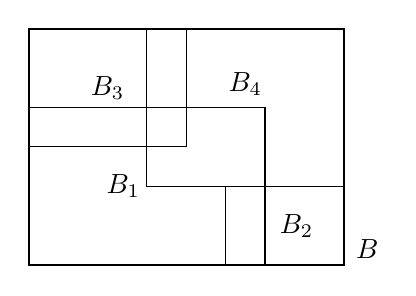
\begin{tikzpicture}
                \draw[style = thick] (0,0) -- (4,0) -- (4,3) -- (0,3) -- cycle;
                \draw (3,0) -- (3,2) -- (0,2);
                \draw (1.5,3) -- (1.5,1) -- (4,1);
                \draw (2.5,0) -- (2.5,1);
                \draw (0,1.5) -- (2,1.5) -- (2,3);
                \node at (4.3,0.2) {$B$};
                \node at (1.2,1) {$B_1$};
                \node at (3.4,0.5) {$B_2$};
                \node at (1,2.25) {$B_3$};
                \node at (2.75,2.3) {$B_4$};
            \end{tikzpicture}
        }
        \qquad
        \subfigure{
            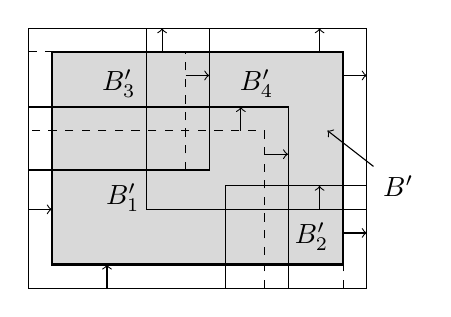
\begin{tikzpicture}
                \draw[style = thick, fill = gray!30!white] (0.3,0.3) -- (4,0.3) -- (4,3) -- (0.3,3) -- cycle;
                \draw (0,0) -- (4.3,0) -- (4.3,3.3) -- (0,3.3) -- cycle;
                \draw (3.3,0) -- (3.3,2.3) -- (0,2.3);
                \draw (1.5,3.3) -- (1.5,1) -- (4.3,1);
                \draw (2.5,0) -- (2.5,1.3) -- (4.3,1.3);
                \draw (0,1.5) -- (2.3,1.5) -- (2.3,3.3);
                \begin{scope}[style = dashed]
                    \draw (0,3) -- (0.3,3);
                    \draw (4,0) -- (4,0.3);
                    \draw (3,0) -- (3,2) -- (0,2);
                    \draw (2,1.5) -- (2,3);
                \end{scope}
                \draw[->] (1,0) -- (1,0.3);
                \draw[->] (0,1) -- (0.3,1);
                \draw[->] (2.7,2) -- (2.7,2.3);
                \draw[->] (3,1.7) -- (3.3,1.7);
                \draw[->] (3.7,3) -- (3.7,3.3);
                \draw[->] (4,2.7) -- (4.3,2.7);
                \draw[->] (1.7,3) -- (1.7,3.3);
                \draw[->] (2,2.7) -- (2.3,2.7);
                \draw[->] (4,0.7) -- (4.3,0.7);
                \draw[->] (3.7,1) -- (3.7,1.3);
                \node (B') at (4.7,1.3) {$B'$};
                \node at (1.2,1.15) {$B_1'$};
                \node at (3.6,0.65) {$B_2'$};
                \node at (1.15,2.6) {$B_3'$};
                \node at (2.9,2.6) {$B_4'$};
                \draw[->] (B') -- (3.8,2);
            \end{tikzpicture}
        }
        \caption{정리 \ref{thm:finiteBorelSpecify}의 증명에서의 집합 $B,\,B_i$ (왼쪽)와 집합 $B',\,B_i'$ (오른쪽).}
    \end{figure}

    이제 $\rho$가 $\mathcal{S}_2$ 위의 \texttt{premeasure}임을 알았으므로 앞서 설명한 바와 같이 이를 $\mathcal{B}_2$ 위의 측도로 확장하는 과정은 자연스럽게 이루어진다. 남은 일은 과연 이러한 확장을 통해 얻은 측도 $\mu$가 정리의 조건을 만족하는지를 확인하는 일인데, 이는 어렵지 않다. 우선 임의의 $x\in\mathbb{N}$에 대해  집합열 $\{B_i\}$를 $B_i:=(x^1-i,\,x^1]\times(x^2-i,\,x^2]$로 두면 이는 $B_i\uparrow(-\infty,\,x^1]\times(-\infty,\,x^2]$인 $\mathcal{S}_2$에 속하는 증가하는 집합열임이 분명하고 $\mu$의 구성 과정으로부터 $\mu(B_i)=\Delta_{B_i}F=F(x^1,\,x^2)-F(x^1-i,\,x^2)-F(x^1,\,x^2-i)+F(x^1-i,\,x^2-i)$이다. 그런데 가정으로부터 $F(x^1-i,\,x^2),\,F(x^1,\,x^2-i)\to0$이고 $F$의 함숫값은 항상 0보다 크거나 같으므로(만약 어떤 $x\in\mathbb{R}^2$에 대해 $F(x)<0$이라면 $F$가 첫 번째 변수에 대해 감소한다는 사실로부터 $0=\lim_{i\to\infty}F(x^1-i,\,x^2)\leq F(x)<0$의 모순이 발생하므로 모든 $x\in\mathbb{R}^2$에 대해 $F(x)\geq0$이다.) $F(x^1-i,\,x^2-i)\leq F(x^1-i,\,x^2)\to0$에서 $F(x^1-i,\,x^2-i)\to0$이 되어 $\mu((-\infty,\,x^1]\times(-\infty,\,x^2])=\lim_{i\to\infty}\mu(B_i)=F(x)$임을 안다.
\end{proof}

이상의 결과는 가측공간 $(\mathbb{R}^n,\,\mathcal{B}_n)$ 위의 유한 측도 $\mu$에 대한 정보는 정리 \ref{thm:distributionProp}에서와 같이 정의된 함수 $F_\mu$에 모두 담겨있음을 뜻한다. 따라서 $F_\mu$만 알고 있다면 원래의 측도 $\mu$를 완벽히 복원해낼 수 있다. 이 놀라운 결과는 한참 후에 \texttt{CDF}를 소개하며 다시 등장할 것이다.

\section{Completion of Measures}

측도가 0인 집합을 생각해보자. 상식적으로, 이 집합의 모든 부분집합은 0의 측도를 가질 것 같지만, 아쉽게도 이가 항상 성립하는 것은 아니다. 어떤 부분집합은 가측이 아닐수도 있기 때문이다. 이렇게 측도가 0인 집합의 부분집합이 가측이 아닐 수도 있다는 사실은 측도론의 전개에 있어 상당히 신경쓰이는 부분이다. 이번 절에서는 \texttt{Lebesgue} 측도의 구성이라는 우리의 목표에서 잠시 옆으로 빠져 이런 문제를 해결하는 방법에 대해 알아본다. 그리고 놀랍게도, 이를 공부함으로써 우리에게 숙제로 남겨진 $\mathcal{M}_n$의 구조에 대한 질문에 어느 정도 만족스러운 답을 할 수 있게 될 것이다.

\begin{definition}
    측도공간 $(X,\,\mathcal{A},\,\mu)$와 부분집합 $N\subseteq X$에 대해 만약 $\mu(A)=0$이고 $N\subseteq A$인 $A\in\mathcal{A}$가 존재하면 이때의 $N$을 \textbf{($\mu$-)영집합(($\mu$-)\texttt{null set})}이라 한다. 또한, 만약 모든 영집합이 $\mathcal{A}$-가측이면 이때의 측도공간 $(X,\,\mathcal{A},\,\mu)$를 \textbf{완비측도공간(\texttt{complete measure space})}이라 한다.
\end{definition}

어떤 측도공간을 완비측도공간으로 만드는 체계적인 방법 즉, 완비화 과정을 찾는 것이 이번 절에서의 우리의 목표이다. 우선 영집합에 대한 몇몇 기본적인 성질들을 보자.

\begin{proposition}\label{prop:nullSet}
    측도공간 $(X,\,\mathcal{A},\,\mu)$에 대해 다음이 성립한다.
    \begin{enumerate}
        \item 영집합 $N$의 임의의 부분집합 $M\subseteq N$도 영집합이다.
        \item 영집합으로 구성된 집합열 $\{N_i\}$에 대해 $\bigcup_{i=1}^\infty N_i$도 영집합이다.
    \end{enumerate}
\end{proposition}

\begin{proof}
    i. 정의로부터 적당한 $A\in\mathcal{A}$가 존재하여 $M\subseteq N\subseteq A$이고 $\mu(A)=0$이므로 이 명제는 자명하다.

    ii. 이번에도 정의로부터 각 $i\in\mathbb{N}$에 대해 적당한 $A_i\in\mathcal{A}$가 존재하여 $N_i\subseteq A_i$이고 $\mu(A_i)=0$이므로 곧 $\bigcup_{i=1}^\infty N_i\subseteq\bigcup_{i=1}^\infty A_i$이고 $\mu(\bigcup_{i=1}^\infty A_i)\leq\sum_{i=1}^\infty\mu(A_i)=0$이 되어 $\bigcup_{i=1}^\infty N_i$도 영집합이다.
\end{proof}

영집합이라는 용어에서 알 수 있듯이 영집합은 `거의' 공집합과 같다. 물론, 아예 아무런 원소를 포함하지 않는 빈 집합인 공집합과 원소를 포함할 수는 있지만 이들이 마치 여기저기 흩어진 점과 같아 의미있는 측도를 이루지 못하는 영집합이 엄밀하게는 서로 다르지만, 이러한 차이점은 많은 경우에 흐려져 영집합을 마치 공집합과 같이 사용하는 경우가 측도론에서는 흔하다. 특히 어떤 성질을 만족하지 않는 경우가 영집합을 이루는 경우, 마치 이런 예외가 아예 없는 것과 같이 생각하곤 한다. 이는 \texttt{Lebesgue} 적분론을 배우기 시작하면 충분히 느낄 수 있으니, 일단은 앞서 설명한 것과 같이 완비화 과정을 정립하는 것에 집중하자.

\begin{proposition}\label{prop:completetionWellDefine1}
    측도공간 $(X,\,\mathcal{A},\,\mu)$와 모든 영집합들의 모임 $\mathcal{N}$에 대해 $\sigma(\mathcal{A}\cup\mathcal{N})=\{A\cup N\subseteq X:A\in\mathcal{A},\,N\in\mathcal{N}\}$이다.
\end{proposition}

\begin{proof}
    표기의 편의를 위해 $\overline{\mathcal{A}}=\{A\cup N\subseteq X:A\in\mathcal{A},\,N\in\mathcal{N}\}$라 하자. 그렇다면 $\emptyset\in\mathcal{A}\cap\mathcal{N}$에서 $\mathcal{A}\cup\mathcal{N}\subseteq\overline{\mathcal{A}}$임은 분명하다. 또한, $\mathcal{A}\cup\mathcal{N}$을 포함하는 모든 $\sigma$-대수가 $\overline{\mathcal{A}}$를 포함해야 함도 분명하므로 $\overline{\mathcal{A}}$가 $\sigma$-대수임을 보이는 것으로 증명은 충분하다. 우선 $\mathcal{A}$가 비어있지 않으므로 $\overline{\mathcal{A}}$도 비어있지 않다. 한편, 임의의 $B\in\overline{\mathcal{A}}$에 대해 적당한 $A\in\mathcal{A},\,N\in\mathcal{N}$이 존재하여 $B=A\cup N$인데, \texttt{WLOG}, 필요하다면 $N$을 $N\setminus A$로 바꾸어 $A$와 $N$이 처음부터 서로소라고 해도 된다. 또한, 정의로부터 적당한 $C\in\mathcal{A}$가 존재하여 $\mu(C)=0$이고 $N\subseteq C$인데, $\mu(C\setminus A)\leq\mu(C)=0$이고 $N\subseteq C\setminus A$이므로 \texttt{WLOG}, 필요하다면 $C$를 $C\setminus A$로 바꾸어 $A$와 $C$가 처음부터 서로소라고 해도 된다. 그렇다면 $B^c=(A\sqcup N)^c=(A\sqcup C)^c\cup(C\setminus N)$에서 $B^c\in\overline{\mathcal{A}}$가 되어 $\overline{\mathcal{A}}$가 여집합에 대해 닫혀있음을 안다. 마지막으로 $\overline{\mathcal{A}}$에 속하는 임의의 집합열 $\{B_i\}$에 대해 이번에도 정의로부터 각 $i\in\mathbb{N}$에 대해 적당한 $A_i\in\mathcal{A},\,N_i\in\mathcal{N}$가 존재하여 $B_i=A_i\cup N_i$로 쓸 수 있다. 그렇다면 $\bigcup_{i=1}^\infty B_i=\bigcup_{i=1}^\infty A_i\cup\bigcup_{i=1}^\infty N_i$에서 명제 \ref{prop:nullSet}의 ii로부터 $\bigcup_{i=1}^\infty N_i$도 영집합이므로 $\bigcup_{i=1}^\infty B_i\in\overline{\mathcal{A}}$가 되어 $\overline{\mathcal{A}}$가 가산 합집합에 대해서도 닫혀있음을 알고, 따라서 이는 $\sigma$-대수이다.
\end{proof}

\begin{proposition}\label{prop:completetionWellDefine2}
    측도공간 $(X,\,\mathcal{A},\,\mu)$에 대해 $A,\,B\in\mathcal{A}$이고 $N,\,M\subseteq X$이 영집합이라 하자. 만약 $A\cup N=B\cup M$이면 $\mu(A)=\mu(B)$이다.
\end{proposition}

\begin{proof}
    집합 $M$이 영집합이므로 적당한 $C\in\mathcal{A}$가 존재하여 $\mu(C)=0$이고 $M\subseteq C$이다. 이는 곧 $A\subseteq A\cup N=B\cup M\subseteq B\cup C$에서 $\mu(A)\leq\mu(B\cup C)\leq\mu(B)+\mu(C)=\mu(B)$임을 의미하는데, 이와 비슷하게 $\mu(A)\geq\mu(B)$도 보일 수 있으므로 증명이 끝난다.
\end{proof}

\begin{theorem}\label{thm:measureCompletion}
    측도공간 $(X,\,\mathcal{A},\,\mu)$와 모든 $\mu$-영집합들의 모임 $\mathcal{N}$에 대해 $\overline{\mathcal{A}}=\{A\cup N\subseteq X:A\in\mathcal{A},\,N\in\mathcal{N}\}$라 하고 함수 $\overline{\mu}:\overline{\mathcal{A}}\to\overline{\mathbb{R}}^+_0$를 $\overline{\mu}:A\cup N\mapsto\mu(A)$로 정의하자. (여기서 $A\in\mathcal{A},\,N\in\mathcal{N}$이다.) 그렇다면 $\overline{\mu}$는 $\mu$의 $\overline{\mathcal{A}}$에서의 측도로의 유일한 확장이고 $(X,\,\overline{\mathcal{A}},\,\overline{\mu})$는 완비측도공간이 된다.
\end{theorem}

\begin{proof}
    명제 \ref{prop:completetionWellDefine1}, \ref{prop:completetionWellDefine2}로부터 $\overline{\mathcal{A}}$는 $\mathcal{A}$를 포함하는 $\sigma$-대수이며 $\overline{\mu}$는 \texttt{well-define}된다. 이제 $\overline{\mu}$가 $\overline{\mathcal{A}}$ 위의 측도임을 보이자. 이를 위해 $\overline{\mathcal{A}}$에 속하는 임의의 서로소인 집합열 $\{B_i\}$를 생각하면 각 $i\in\mathbb{N}$에 대해 적당한 $A_i\in\mathcal{A},\,N_i\in\mathcal{N}$가 존재하여 $B_i=A_i\cup N_i$이고 $\{A_i\}$와 $\{N_i\}$가 명백히 서로소이므로, $\overline{\mu}(\bigsqcup_{i=1}^\infty B_i)=\overline{\mu}(\bigsqcup_{i=1}^\infty A_i\cup\bigsqcup_{i=1}^\infty N_i)=\mu(\bigsqcup_{i=1}^\infty A_i)=\sum_{i=1}^\infty\mu(A_i)=\sum_{i=1}^\infty\overline{\mu}(B_i)$이다. 한편, $\overline{\mu}(\emptyset)=0$임은 분명하므로 $\overline{\mu}$는 명백히  $\overline{\mathcal{A}}$ 위의 측도이다. 그렇다면 $\emptyset$이 $\mu$-영집합이라는 사실로부터  $\overline{\mu}$가 $\mu$의 확장임은 자명하다.

    다음으로, 측도공간 $(X,\,\overline{\mathcal{A}},\,\overline{\mu})$의 완비성을 보이자. 이를 위해 임의의 $B\in\overline{\mathcal{A}}$를 택하여 $\overline{\mu}(B)=0$이라 하면, 적당한 $A\in\mathcal{A},\,N\in\mathcal{N}$이 존재하여 $B=A\cup N$이고 $\mu(A)=\overline{\mu}(B)=0$이다. 이는 $A\in\mathcal{N}$임을 뜻하므로 임의의 $M\subseteq B$에 대해 $M\in\mathcal{N}\subseteq\overline{\mathcal{A}}$이고, 곧 $B$의 임의의 부분집합이 $\overline{\mathcal{A}}$-가측이 되어 $(X,\,\overline{\mathcal{A}},\,\overline{\mu})$가 완비측도공간임을 안다.

    마지막으로 유일성을 보이기 위해 $\nu$를 $\mu$의 $\overline{\mathcal{A}}$에서의 측도로의 확장이라 하고 $B\in\overline{\mathcal{A}}$를 임의로 하나 택하자. 그렇다면 적당한 $A\in\mathcal{A}$와 $N\in\mathcal{N}$이 존재하여 $B=A\cup N$이고, 다시 적당한 $C\in\mathcal{A}$가 존재하여 $N\subseteq C$이고 $\mu(C)=0$이다. 이로부터 $\nu(B)=\nu(A\cup N)\geq\nu(A)=\mu(A)=\overline{\mu}(B)$이고 $\nu(B)=\nu(A\cup N)\leq\nu(A)+\nu(N)\leq\nu(A)+\nu(C)=\mu(A)=\overline{\mu}(B)$에서 $\nu=\overline{\mu}$가 되어 원하던 유일성을 얻는다.
\end{proof}

이상으로부터 다음과 같은 \texttt{well-define}된 완비화를 얻을 수 있다.

\begin{definition}
    측도공간 $(X,\,\mathcal{A},\,\mu)$와 모든 $\mu$-영집합들의 모임 $\mathcal{N}$에 대해 $\overline{\mathcal{A}}=\{A\cup N\subseteq X:A\in\mathcal{A},\,N\in\mathcal{N}\}$라 하고 함수 $\overline{\mu}:\overline{\mathcal{A}}\to\overline{\mathbb{R}}^+_0$를 $\overline{\mu}:A\cup N\mapsto\mu(A)$로 정의하자. (여기서 $A\in\mathcal{A},\,N\in\mathcal{N}$이다.) 이때의 완비측도공간 $(X,\,\overline{\mathcal{A}},\,\overline{\mu})$를 측도공간 $(X,\,\mathcal{A},\,\mu)$의 \textbf{완비화(\texttt{completion})}라 한다.
\end{definition}

위의 정의에서와 같이 일반적으로 측도공간의 완비화를 통해 얻는 $\sigma$-대수와 측도는 각각 원래의 $\sigma$-대수와 측도에 \texttt{overline}을 그어 표기한다. 나중을 위해 정리 하나를 소개한다.

\begin{theorem}\label{thm:Complete2}
    측도공간 $(X,\,\mathcal{A},\,\mu)$와 부분집합 $A\subseteq X$에 대해 $A\in\overline{\mathcal{A}}$일 필요충분조건은 적당한 $B,\,C\in\mathcal{A}$가 존재하여 $B\subseteq A\subseteq C$이고 $\mu(C\setminus B)=0$인 것이다.
\end{theorem}

\begin{proof}
    충분조건임을 보이기 위해 $A\in\overline{\mathcal{A}}$라 하면 적당한 $B\in\mathcal{A}$와 영집합 $N\subseteq X$이 존재하여 $A=B\cup N$이며, 다시 적당한 $D\in\mathcal{A}$가 존재하여 $N\subseteq D$이고 $\mu(D)=0$이다. 이제 $C=B\cup D$라 하면 $B\subseteq A\subseteq C$이고 $\mu(C\setminus B)\leq\mu(D)=0$이 되어 충분조건임이 보여진다. 다음으로, 필요조건임을 보이기 위해 적당한 $B,\,C\in\mathcal{A}$가 존재하여 $B\subseteq A\subseteq C$이고 $\mu(C\setminus B)=0$이라 하자. 그렇다면 $A=(A\setminus B)\sqcup B$이고 $A\setminus B\subseteq C\setminus B$에서 $A\setminus B$가 영집합이므로 $A\in\overline{\mathcal{A}}$가 되어 필요조건임도 보여진다.
\end{proof}

이번 절의 남은 부분에서는 앞서 예고했던 바와 같이 이러한 완비화가 $\mathcal{M}_n$의 구조에 대한 질문으로 어떻게 연결되는지 살펴보려고 한다. 우선 \texttt{Carath\'eodory}의 확장정리로 잠시 돌아가자.

\begin{theorem}\label{thm:CaratheodoryComplete}
    공집합이 아닌 집합 $X$ 위의 대수 $\mathcal{A}$에 대해 $\rho$를 $\mathcal{A}$ 위의 \texttt{premeasure}라 하고, $\mathcal{M}$을 모든 $\rho^*$-가측집합들의 모임이라 하자. 또한 $\mu$를 $\rho$의 \texttt{Carath\'eodory} 확장이라 하면 $(X,\,\mathcal{M},\,\mu)$는 완비측도공간이다.
\end{theorem}

\begin{proof}
    집합 $N\subseteq X$이 영집합이라 하면 정의로부터 적당한 $A\subseteq\mathcal{M}$가 존재하여 $\mu(A)=0$이고 $N\subseteq A$이므로 임의의 $S\subseteq X$에 대해 $\rho^*(S\cap N)+\rho^*(S\cap N^c)\leq\rho^*(A)+\rho^*(S\cap N^c)=\mu(A)+\rho^*(S\cap N^c)=\rho^*(S\cap N^c)\leq\rho^*(S)$가 성립하여 $N\in\mathcal{M}$이고, 곧 $(X,\,\mathcal{M},\,\mu)$는 완비측도공간임을 안다.
\end{proof}

따라서 \texttt{Carath\'eodory}의 확장정리를 통해 얻는 모든 측도공간은 완비성을 가지고, 특히 \texttt{Lebesgue} 측도공간은 완비측도공간이다. 그렇다면 조심스럽게, 어쩌면 \texttt{Lebesgue} 측도공간이 \texttt{Borel} 측도공간의 완비화가 아닐까하는 추측을 해 볼 수도 있다. 이 추측의 결론은 다음과 같다.

\begin{theorem}\label{thm:LebesgueComplete}
    \texttt{Lebesgue} 측도공간 $(\mathbb{R}^n,\,\mathcal{M}_n,\,\lambda_n)$은 \texttt{Borel} 측도공간 $(\mathbb{R}^n,\,\mathcal{B}_n,\,\mu_n)$의 완비화이다. 즉, $(\mathbb{R}^n,\,\mathcal{M}_n,\,\lambda_n)=(\mathbb{R}^n,\,\overline{\mathcal{B}_n},\,\overline{\mu_n})$.
\end{theorem}

\begin{proof}
    정리 \ref{thm:measureCompletion}로부터 완비화를 통해 얻는 $\sigma$-대수로의 측도의 확장은 유일하므로 $\overline{\mathcal{B}_n}=\mathcal{M}_n$을 보이는 것으로 충분하다. 우선 $\overline{\mathcal{B}_n}\subseteq\mathcal{M}_n$부터 보이자. 임의의 집합 $A\in\overline{\mathcal{B}_n}$를 택하면 적당한 $B\in\mathcal{B}_n$와 $\mu_n$-영집합 $N\subseteq\mathbb{R}^n$이 존재하여 $A=B\cup N$이고, 다시 적당한 $C\in\mathcal{B}_n$가 존재하여 $N\subseteq C$이고 $\mu_n(C)=0$이다. 이제 \texttt{Lebesgue} 측도공간은 정리 \ref{thm:CaratheodoryComplete}로부터 완비측도공간이므로 $N\in\mathcal{M}_n$이 되어 $A=B\cup N\in\mathcal{M}_n$에서 곧 $\overline{\mathcal{B}_n}\subseteq\mathcal{M}_n$이다.

    역의 포함 관계를 보이는 것은 조금 더 복잡하다. 임의의 $A\in\mathcal{M}_n$를 택하고 먼저 $\lambda_n(A)<\infty$인 경우를 생각하자. 이 경우, 정리 \ref{thm:LebesgueRegular}로부터 각 $i\in\mathbb{N}$에 대해 \texttt{compact}한 $K_i\in\mathcal{B}_n$와 열린 $U_i\in\mathcal{B}_n$가 존재하여 $K_i\subseteq A\subseteq U_i$이고 $\lambda_n(A)-1/i<\lambda_n(K_i)\leq\lambda_n(A)\leq\lambda_n(U_i)<\lambda_n(A)+1/i$이므로 이들로써 집합열 $\{K_i\},\,\{U_i\}$를 구성할 수 있으며 \texttt{WLOG}, 필요하다면 각각의 항을 $F_i:=\bigcup_{j=1}^iK_j,\,V_i:=\bigcap_{j=1}^iU_j$로 바꾸어 $\{K_i\},\,\{U_i\}$ 각각을 증가하고 감소하는 집합열이라 해도 된다. 그렇다면 그 구성으로부터 $\{K_i\},\,\{U_i\}$는 각각 $K:=\bigcup_{i=1}^\infty K_i,\,U:=\bigcap_{i=1}^\infty U_i$로 수렴하고, 곧 $K\subseteq A\subseteq U$이며 $\lambda_n(K)=\lambda_n(A)=\lambda_n(U)$이다. 따라서 $\mu_n(U\setminus K)=\lambda_n(U)-\lambda_n(K)=0$이 되어 정리 \ref{thm:Complete2}로부터 $A\in\overline{\mathcal{B}_n}$임을 안다. 한편, $\lambda_n(A)=\infty$인 경우에는 각 $i\in\mathbb{N}$에 대해 $A\cap B(i)$가 유계이므로 정리 \ref{thm:boundedMeasure}로부터 이는 유한한 \texttt{Lebesgue} 측도를 가지고, 곧 앞선 결과로부터 $A\cap B(i)\in\overline{\mathcal{B}_n}$이 되어 적당한 $B_i\in\mathcal{B}_n$과 $\mu_n$-영집합 $N_i\subseteq\mathbb{R}^n$가 존재하여 $A\cap B(i)=B_i\cup N_i$이다. 이로부터 $A=\bigcup_{i=1}^\infty[A\cap B(i)]=\bigcup_{i=1}^\infty B_i\cup\bigcup_{i=1}^\infty N_i$인데 명제 \ref{prop:nullSet}의 ii에서 $\bigcup_{i=1}^\infty N_i$도 $\mu_n$-영집합이므로 $A\in\overline{\mathcal{B}_n}$임을 안다. 곧 어느 경우에나 $A\in\overline{\mathcal{B}_n}$이므로 $\overline{\mathcal{B}_n}\supseteq\mathcal{M}_n$이 되어 증명이 끝난다.
\end{proof}

실로 놀라운 결과가 아닐 수 없다! 우리는 $\mathcal{M}_n$의 구조를 전혀 모르는 상태에서 단지 이가 너무 크다는 생각에 이 중에서 쓸만하다고 생각되는 극히 일부의 집합만 뽑아내어 $\mathcal{B}_n$을 구성했는데, $\mathcal{B}_n$은 정말로 $\mathcal{M}_n$에서 중요한 원소들로만 이루어진 알짜배기 $\sigma$-대수였던 것이다.

\section{Measurable Functions}

이제 \texttt{Lebesgue} 측도를 다른 방법으로 다시 구성하는 것으로 본 장의 후반부를 시작한다. \texttt{Lebesgue} 측도의 두 번째 구성 또한 기본적으로는 확장을 이용한 방법으로, 이번에는 마치 $n$개의 $\mathbb{R}$에 \texttt{Cartesian} 곱을 취하여 $\mathbb{R}^n$을 얻는 것과 비슷하게 $n$개의 \texttt{Lebesgue} 측도공간 $(\mathbb{R},\,\mathcal{M}_1,\,\lambda_1)$에 적당한 곱연산을 취하여 $(\mathbb{R}^n,\,\mathcal{M}_n,\,\lambda_n)$을 얻어보려고 한다. 다만, 이번에도 $\mathcal{M}_n$이 너무 거대한 탓에 곱연산을 취한다고 해서 곧바로 $\mathcal{M}_n$을 얻지는 못하는데, 다행히 이는 완비화를 통해 해결할 수 있다. 이러한 방법은 \texttt{Carath\'eodory}의 확장정리를 비롯한 확장정리들을 사용한 방법보다 훨씬 더 직관적인 방법인데, 그럼에도 불구하고 이 방법을 두 번째로 소개하는 까닭은 이때 사용할 `적당한 곱연산'을 정의하기가 꽤나 어렵기 때문이다. 마치 배보다 배꼽이 더 큰 격이다. 특히, 이 곱연산을 정의하려면 \texttt{Lebesgue} 적분론의 전개가 반드시 필요하므로 일단은 \texttt{Lebesgue} 적분론에 집중하도록 하고, 이 과정이 끝나면 다시 원래의 목표로 돌아와 \texttt{Lebesgue} 측도의 두 번째 구성을 마무리하도록 하겠다.

앞서 초록에서 지적한 바와 같이 \texttt{Lebesgue} 적분론은 우리가 측도론을 배우는 주된 이유 중 하나이다. 물론, \texttt{Lebesgue} 적분론에서 극한과 적분의 상호작용이 \texttt{Riemann} 적분론에서보다 자연스럽다는 것도 \texttt{Lebesgue} 적분론의 장점 중 하나이지만, \texttt{Lebesgue} 적분론의 가장 큰 수학적 의의는 측도가 정의되는 임의의 공간에서 적분론을 전개할 수 있도록 적분의 개념을 확장했다는 데 있다. 우리가 $\mathbb{R}^2$나 $\mathbb{R}^3$에 한정되었던 넓이나 부피의 개념을 일반적인 공간으로 일반화하여 측도의 개념을 정립하였으니 어찌보면 이는 당연한 수순이다.

\texttt{Lebesgue} 적분론을 정립하기 위한 준비로서, 과연 어떤 함수를 적분의 대상으로 삼아야 하는지에 대해 생각해보자. 당연히, 더 이상 함수의 정의역이 $\mathbb{R}^n$의 부분집합일 필요가 없다. 정의역에서 적당한 측도가 정의되기만 하면 충분하다. 한편, \texttt{Riemann} 적분론에서 \texttt{properly} 적분가능한 함수는 반드시 유계여야 했는데, 이 또한 왠지 불필요하게 과도한 제한이라 생각된다. 결론부터 말하자면, \texttt{Lebesgue} 적분론에서 적분의 대상이 되는 함수는 가측함수들이다. (가측함수라고 해서 모두 적분가능하다는 뜻이 아니다. 마치 \texttt{Riemann} 적분론에서 유계함수라고 해서 모두 적분가능하지는 않은 것처럼 \texttt{Lebesgue} 적분론에서도 적분불가능한 가측함수가 얼마든지 있다.) 이번 절에서는 이러한 가측함수에 대해 알아보도록 하겠다.

\begin{definition}
    가측공간 $(X,\,\mathcal{A}),\,(Y,\,\mathcal{B})$와 함수 $f:X\to Y$를 생각하자. 만약 임의의 $A\in\mathcal{B}$에 대해 $f^{-1}(A)\in\mathcal{A}$이면 이때의 $f$를 \textbf{($\mathcal{A}/\mathcal{B}$-)가측함수(($\mathcal{A}/\mathcal{B}$-)\texttt{measurable function})}라 한다. 특히, 만약 $\mathcal{A}$가 \texttt{Borel} $\sigma$-대수이면 이때의 $f$를 \textbf{\texttt{Borel} 함수(- \texttt{function})}라 한다.
\end{definition}

\begin{theorem}\label{thm:generatorMeasurable}
    가측공간 $(X,\,\mathcal{A}),\,(Y,\,\mathcal{B})$와 함수 $f:X\to Y$에 대해 $\mathcal{C}$를 $\mathcal{B}$의 생성자라 하면 $f$가 가측일 필요충분조건은 임의의 $A\in\mathcal{C}$에 대해 $f^{-1}(A)\in\mathcal{A}$인 것이다.
\end{theorem}

\begin{proof}
    충분조건임은 정의로부터 자명하므로 필요조건임만 보이면 된다. 이를 위해 $\mathcal{D}=\{A\subseteq Y:f^{-1}(A)\in\mathcal{A}\}$를 생각하면 가정으로부터 $\mathcal{C}\subseteq\mathcal{D}$에서 $\mathcal{D}$는 비어있지 않다. 또한, 임의의 $A\in\mathcal{D}$에 대해 $f^{-1}(A^c)=[f^{-1}(A)]^{-1}\in\mathcal{A}$에서 $A^c\in\mathcal{D}$가 되어 $\mathcal{D}$는 여집합에 대해 닫혀있다. 마지막으로 $\mathcal{D}$에 속하는 임의의 집합열 $\{A_i\}$에 대해 $f^{-1}(\bigcup_{i=1}^\infty A_i)=\bigcup_{i=1}^\infty f^{-1}(A_i)\in\mathcal{A}$에서 $\bigcup_{i=1}^\infty A_i\in\mathcal{D}$이므로 $\mathcal{D}$는 가산 합집합에 대해서도 닫혀있어서 곧 이는 $\sigma$-대수이고 $\mathcal{B}\subseteq\mathcal{D}$가 되어 증명이 끝난다.
\end{proof}

적분론에서는 이론 전개상의 편의를 위해 실수체계에 $\pm\infty$를 추가하는 것이 편하다. 이렇게 실수에 $\pm\infty$를 추가한 수 체계를 \textbf{확장된 실수(\texttt{extended real number})}라 하며 $\overline{\mathbb{R}}$로 쓴다. 우리가 $\mathbb{R}$에서 성립하는 것으로 알고있는 거의 대부분의 성질들, 예컨대 \texttt{LUBP}, \texttt{GLBP}, \texttt{MSP} 따위의 성질들은 $\overline{\mathbb{R}}$에서도 그대로 (사실은 더 잘) 성립한다. 다만, $\overline{\mathbb{R}}$에서는 $\mathbb{R}$에서의 표준 거리함수가 더 이상 제 역할을 하지 못하므로 (당장 $d(-\infty,\,\infty)$를 뭐라고 해야 할지부터가 대략 난감하다.) $\overline{\mathbb{R}}$에서의 열림과 닫힘을 정의하기 위해서는 새로운 아이디어가 필요하다. 여기에서는 위상수학의 내용을 피하기 위해 결론만 받아들이도록 하자. 우리는 집합 $U\subseteq\overline{\mathbb{R}}$가 적당한 $x,\,y\in\mathbb{R}$에 대해 $(x,\,y),\,(x,\,\infty],\,[-\infty,\,y)$ 중 하나로 표현되는 구간들의 가산 합집합으로 표현되면 이때의 $U$를 열린집합이라 정의한다. 이제 닫힌집합의 정의는 $\mathbb{R}$에서와 마찬가지이다. 한편, $\mathbb{R}$에서의 열린집합이 유계인 열린구간의 가산 합집합으로 표현된다는 점을 상기하면(각주 \ref{note:countableOpenBox} 참조.), 이는 $\overline{\mathbb{R}}$에서도 여전히 열려있음을 알 수 있고, 곧 $\mathcal{U},\,\mathcal{U}'$를 각각 $\mathbb{R}$과 $\overline{\mathbb{R}}$에서의 모든 열린집합의 모임이라 하면 $\mathcal{U}\subseteq\mathcal{U}'$이 성립한다.\footnotemark

이제 $\mathcal{B}_1$을 정의한 것과 비슷하게 $\overline{\mathbb{R}}$ 위의 $\sigma$-대수 $\mathcal{B}_1'$을 $\mathcal{U}'$이 생성하는 $\sigma$-대수로 정의하자.\footnotemark 그렇다면 $\mathcal{U}\subseteq\mathcal{U}'$에서 $\mathcal{B}_1\subseteq\mathcal{B}_1'$이 성립한다. 사실, 대부분의 경우 \texttt{WLOG}, 실함수의 공역을 $\overline{\mathbb{R}}$라 해도 되므로 $\mathcal{B}_1$과 $\mathcal{B}_1'$을 엄밀하게 구분해야 할 필요가 그렇게 많지 않고, 따라서 표기를 남용하여 $\mathcal{B}_1'$을 그냥 $\mathcal{B}_1$로 쓴다. 나아가 정리 \ref{thm:BorelGen1}, \ref{thm:BorelGen2}, \ref{thm:BorelGen3}의 증명을 비슷하게 반복하면 $\overline{\mathbb{R}}$ 위의 $\mathcal{B}_1$에 대해 다음 결과를 얻는다.

\vspace{6pt}
\noindent{\ttfamily\bfseries Theorem \ref{thm:BorelGen3}$^\circ$} 집합족 $\mathcal{C}$를 어떤 $x\in\mathbb{R}$에 대해 $[-\infty,\,x]$로 표현되는 모든 구간의 모임이라 하면 이는 $\mathcal{B}_1$의 생성자이다.

\vspace{6pt}
한편, 앞서 가측함수를 굉장히 일반적으로 정의했지만, 적분론의 전개를 목표로 하는 우리는 함수의 공역이 $\overline{\mathbb{R}}$이거나 $\mathbb{R}^n$인 두 가지 경우에 특히 관심이 있다. 그리고 예외적으로, $\overline{\mathbb{R}}$이나 $\mathbb{R}^n$이 함수의 공역을 쓰인 경우, 여기에는 \texttt{Lebesgue} 측도가 아닌 \texttt{Borel} 측도가 주어진 것으로 가정한다. 따라서 다음 보조정리가 자주 쓰인다.

\begin{corollary}
    가측공간 $(X,\,\mathcal{A})$에서 정의된 함수 $f:X\to\mathbb{R}^n$(혹은 $f:X\to\overline{\mathbb{R}}$)에 대해 $f$가 가측일 필요충분조건은 임의의 $x\in\mathbb{R}^n$(혹은 $x\in\mathbb{R}$)에 대해 $f^{-1}(\prod_{i=1}^n(-\infty,\,x_i])\in\mathcal{A}$(혹은 $f^{-1}([-\infty,\,x])\in\mathcal{A}$)인 것이다.
\end{corollary}

\begin{proof}
    이는 정리 \ref{thm:BorelGen3}$^\circ$, \ref{thm:generatorMeasurable}로부터 자명하다.
\end{proof}

정의만 가지고는 어떤 함수가 가측인지의 여부를 직접 판단하는 것은 쉬운 일이 아니므로 이에 도움이 될 만한 정리들을 다수 소개한다.

\begin{proposition}\label{prop:indicatorMeasurable}
    가측공간 $(X,\,\mathcal{A})$에 대해 집합 $A\subseteq X$가 가측일 필요충분조건은 $\ind_A$가 가측인 것이다.
\end{proposition}

\begin{proof}
    정의로부터 $\ind_A$가 가측인 것과 임의의 $x\in\mathbb{R}$에 대해 집합
    \begin{equation*}
        \ind_A^{-1}([-\infty,\,x])=
        \begin{dcases*}
            X&$x\geq1$인 경우\\
            A^c&$0\leq x<1$인 경우\\
            \emptyset&\texttt{ow.}
        \end{dcases*}
    \end{equation*}
    이 가측인 것은 동치이고, 이는 다시 $A$가 가측이라는 것과 동치이므로 이 명제는 자명하다.
\end{proof}

\begin{theorem}\label{thm:compositionMeasurable}
    가측공간 $(X,\,\mathcal{A})$에서 정의된 가측함수 $f:X\to\mathbb{R}^m$와 \texttt{Borel} 함수 $g:\mathbb{R}^m\to\mathbb{R}^n$(혹은 $g:\mathbb{R}^m\to\overline{\mathbb{R}}$)에 대해 합성 $g\circ f$는 가측이다.
\end{theorem}

\begin{proof}
    임의의 $x\in\mathbb{R}^n$를 택하면 가정으로부터 $g^{-1}((-\infty,\,x])$가 \texttt{Borel}이고, 따라서 $(g\circ f)^{-1}((-\infty,\,x])=f^{-1}(g^{-1}((-\infty,\,x]))$가 가측이 되어 $g\circ f$가 가측임을 안다.
    
    한편, $g:\mathbb{R}^m\to\overline{\mathbb{R}}$의 경우에도 이와 비슷하게 보일 수 있다.
\end{proof}

위의 정리에서 함수 $g$가 \texttt{Borel}이라는 조건은 필수적이다. 만약 $g$가 단지 가측함수에 그친다면, $f,\,g$는 모두 가측이지만 그 합성이 가측이 아닌 반례가 존재한다.\footnotemark

\begin{theorem}\label{thm:continuousMeasurable}
    모든 연속함수 $f:\mathbb{R}^m\to\mathbb{R}^n$는 \texttt{Borel}이다.
\end{theorem}

\begin{proof}
    임의의 $x\in\mathbb{R}^n$에 대해 $(-\infty,\,x]$가 닫혀있으므로 그 역상 $f^{-1}((-\infty,\,x])$도 닫혀있고, 곧 \texttt{Borel}이므로 $f$는 \texttt{Borel}이다.
\end{proof}

\begin{theorem}\label{thm:componentMeasurable}
    가측공간 $(X,\,\mathcal{A})$에서 정의된 함수 $f:X\to\mathbb{R}^n$에 대해 $f$가 가측일 필요충분조건은 $f$의 각 성분 $f_1,\,\cdots,\,f_n:X\to\mathbb{R}$이 가측인 것이다.
\end{theorem}

\begin{proof}
    충분조건임을 보이기 위해 임의의 $x\in\mathbb{R}$를 택하면 각 $i\leq n$에 대해 $\mathbb{R}^{i-1}\times(-\infty,\,x]\times\mathbb{R}^{n-i}$이 닫혀있으므로 곧 \texttt{Borel}이 되어 가정으로부터 $f_i^{-1}((-\infty,\,x])=f^{-1}(\mathbb{R}^{i-1}\times(-\infty,\,x]\times\mathbb{R}^{n-i})$가 가측이고, 따라서 $f_i$가 가측이 되어 충분조건임이 보여진다. 반대로, 필요조건임을 보이기 위해 임의의 $x\in\mathbb{R}^n$를 택하면 가정으로부터 모든 $i\leq n$에 대해 $f_i^{-1}((-\infty,\,x_i])$가 가측이므로 $f^{-1}((-\infty,\,x])=\bigcap_{i=1}^nf_i^{-1}((-\infty,\,x_i])$가 가측이고, 따라서 $f$가 가측이 되어 필요조건임이 보여진다.
\end{proof}

\begin{theorem}\label{thm:basicOpMeasurable}
    가측공간 $(X,\,\mathcal{A})$에서 정의된 가측함수 $f,\,g:X\to\mathbb{R}^n$(혹은 $f,\,g:X\to\overline{\mathbb{R}}$)와 가측함수 $h:X\to\mathbb{R}$(혹은 $h:X\to\overline{\mathbb{R}}$)에 대해 $f\pm g,\,hf,\,f/h$는 모두 가측이다. 단,연산의 과정에서 $0$으로 나누게 되거나 $\infty-\infty,\,\infty/\infty,\,0\cdot\infty$와 같은 부정형이 등장하여 그 결과가 \texttt{well-define}되지 않는 경우 이를 $c\in\mathbb{R}$와 같은 \texttt{dummy value}로 두는 관례를 전제하자.
\end{theorem}

\begin{proof}
    각 $i\leq n$에 대해 정리 \ref{thm:componentMeasurable}로부터 $f_i,\,g_i$는 가측이고, 함수 $+,\,-,\,\cdot:\mathbb{R}^2\to\mathbb{R}$가 모두 연속함수이므로 정리 \ref{thm:continuousMeasurable}로부터 이들은 \texttt{Borel}이다. 그렇다면 정리 \ref{thm:compositionMeasurable}로부터 $f_i\pm g_i,\,hf_i$가 모두 가측이며, 다시 정리 \ref{thm:componentMeasurable}에서 $f\pm g,\,hf$가 가측임을 안다. 마지막으로, $f/h$가 가측임을 보이기 위해서는 $1/h$가 가측임을 보이는 것으로 충분한데, $h^{-1}(0)=\emptyset$인 경우에는
    \begin{equation*}
        (1/h)^{-1}((-\infty,\,x])=
        \begin{dcases*}
            h^{-1}((-\infty,\,0))\cup h^{-1}([1/x,\,\infty))&$x>0$인 경우\\
            h^{-1}((-\infty,\,0))&$x=0$인 경우\\
            h^{-1}([1/x,\,0))&\texttt{ow.}
        \end{dcases*}
    \end{equation*}
    이므로 $1/h$는 가측이다. 이제 일반적인 $h$에 대해서도 $A=h^{-1}(0)$에 대해 이가 닫힌집합이므로 곧 \texttt{Borel}이고 $1/h=(1/h)\ind_{X\setminus A}+c\ind_A$에서 $1/h$가 가측이 되어 증명이 끝난다. 한편, $f,\,g,\,h:X\to\overline{\mathbb{R}}$인 경우에도 비슷하게 하면 된다.
\end{proof}

\begin{theorem}\label{thm:limitMeasurable}
    가측공간 $(X,\,\mathcal{A})$에서 정의된 가측함수 $f_i:X\to\overline{\mathbb{R}}$의 열 $\{f_i\}$에 대해 다음이 성립한다.
    \begin{enumerate}
        \item 함수 $\sup_{i\in\mathbb{N}}f_i,\,\inf_{i\in\mathbb{N}}f_i,\,\limsup_{i\to\infty}f_i,\,\liminf_{i\to\infty}f_i$는 모두 가측이다.
        \item 만약 모든 $x\in X$에 대해 $\lim_{i\to\infty}f_i(x)$가 존재하면 이는 가측이다.
        \item 집합 $\{x\in X:\{f_i(x)\}\textrm{가 수렴}\}$이 가측이다.
        \item 임의의 가측인 $f:X\to\overline{\mathbb{R}}$에 대해 집합 $\{x\in X:f_i(x)\to f(x)\}$가 가측이다.
    \end{enumerate}
    한편, 가측함수 $f_i:X\to\mathbb{R}^n$의 열 $\{f_i\}$에 대해서도 i을 제외한 나머지 성질들이 성립한다. 다만, iv의 경우 가측함수 $f:X\to\mathbb{R}^n$에 대해 성립한다
\end{theorem}

\begin{proof}
    i. 임의의 $x\in\mathbb{R}$에 대해 $\{y\in X:\sup_{i\in\mathbb{N}}f_i(y)\leq x\}=\bigcap_{i=1}^\infty f_i^{-1}([-\infty,\,x])$가 가측이므로 곧 $\sup_{i\in\mathbb{N}}f_i$가 가측이고, 비슷하게 $\inf_{i\in\mathbb{N}}f_i$도 가측임을 보일 수 있다. 한편, $\limsup_{i\to\infty}f_i=\inf_{j\in\mathbb{N}}\sup_{i\geq j}f_i$이고 $\liminf_{i\to\infty}f_i=\sup_{j\in\mathbb{N}}\inf_{i\geq j}f_i$이므로 앞선 결과로부터 이들 또한 가측이다.

    ii. 이는 $\lim_{i\to\infty}f_i=\limsup_{i\to\infty}f_i=\liminf_{i\to\infty}f_i$에서 자명하다.

    iii. 정리에서 주어진 집합이 곧 $\{x\in X:\limsup_{i\to\infty}f_i(x)=\liminf_{i\to\infty}f_i(x)\}$이므로 자명하다.

    iv.  정리에서 주어진 집합이 곧 $\{x\in X:\limsup_{i\to\infty}f_i(x)=\liminf_{i\to\infty}f_i(x)=f(x)\}$이므로 자명하다.

    한편, 가측함수 $f_i:X\to\mathbb{R}^n$의 열 $\{f_i\}$와 가측함수 $f:X\to\mathbb{R}^n$의 경우에는 앞선 결과를 성분별로 적용하면 된다.
\end{proof}

이전 절에서 공집합과 영집합 간의 차이가 흐려져 마치 공집합과 영집합을 같은 것처럼 생각하는 경우가 많다고 하였는데, 이를 조금 더 명확히 하기 위해 `거의 어디서나'라는 개념을 소개한다. 이 뭔가 굉장히 수학스럽지 않은 개념은 측도론의 발전이 낳은 사고방식 중 하나이다.

\begin{definition}
    측도공간 $(X,\,\mathcal{A},\,\mu)$에서 적당한 영집합 $N\subseteq X$이 존재하여 어떤 성질이 모든 $x\in X\setminus N$에 대해 성립한다면 그 성질은 $X$의 \textbf{($\mu$-)거의 어디서나(($\mu$-)\texttt{almost everywhere})} 혹은 \textbf{($\mu$-)거의 대부분의 $x\in X$에 대해(($\mu$-)\texttt{almost every} $x\in X$)} 성립한다고 한다.
\end{definition}

어떤 성질 $P$가 거의 어디서나 성립한다는 것을 때로는 $P$ (\texttt{ae.})라 줄여 간단히 표기할 때도 있다. 한편, 거의 어디서나 성립하는 성질 중 가운데 특히 자주 쓰이는 것이 바로 \textbf{거의 어디서나 같다(\texttt{almost everywhere equality})}는 개념이다.

\begin{proposition}
    거의 어디서나 같다는 관계는 동치관계이다. 즉, 측도공간 $(X,\,\mathcal{A},\,\mu)$와 집합 $Y$, 함수 $f,\,g,\,h:X\to Y$에 대해 다음이 성립한다.
    \begin{enumerate}
        \item (반사성) $f=f$ (\texttt{ae.})
        \item (대칭성) $f=g$ (\texttt{ae.})이면 $g=f$ (\texttt{ae.})이다.
        \item (전이성) $f=g$ (\texttt{ae.})이고 $g=h$ (\texttt{ae.})이면 $f=h$ (\texttt{ae.})이다.
    \end{enumerate}
\end{proposition}

\begin{proof}
    반사성과 대칭성은 자명하므로 전이성만 보이면 되는데, $\{x\in X:f(x)\ne h(x)\}\subseteq\{x\in X:f(x)\ne g(x)\}\cup\{x\in X:g(x)\ne h(x)\}$에서 우변의 두 집합이 모두 영집합이므로 좌변의 집합도 영집합이 되어 전이성이 성립함을 알고, 증명이 끝난다.
\end{proof}

\begin{theorem}\label{thm:equalityAeMeasurable}
    완비측도공간 $(X,\,\mathcal{A},\,\mu)$, 가측공간 $(Y,\,\mathcal{B})$와 함수 $f,\,g:X\to Y$에 대해 만약 $f$가 가측이고 $f=g$ (\texttt{ae.})이면 $g$도 가측이다.
\end{theorem}

\begin{proof}
    임의의 $A\in\mathcal{B}$를 택하고 $N=f^{-1}(A)\triangle g^{-1}(A)$라 하면 $N\subseteq\{x\in X:f(x)\ne g(x)\}$이므로 이는 가측이고, 따라서 $g^{-1}(A)=f^{-1}(A)\triangle N$도 가측이 되어 $g$가 가측임을 안다.
\end{proof}

\begin{theorem}\label{thm:limitAeMeasurable}
    완비측도공간 $(X,\,\mathcal{A},\,\mu)$에서 정의된 가측함수 $f_i:X\to\mathbb{R}^n$(혹은 $f_i:X\to\overline{\mathbb{R}}$)의 열 $\{f_i\}$, 함수 $f:X\to\mathbb{R}^n$(혹은 $f:X\to\overline{\mathbb{R}}$)에 대해 만약 $f_i\to f$ (\texttt{ae.})이면 $f$도 가측이다.
\end{theorem}

\begin{proof}
    집합 $N=\{x\in X:f_i(x)\not\to f(x)\}$를 생각하여 함수 $g_i:X\to\mathbb{R}^n$(혹은 $g_i:X\to\overline{\mathbb{R}}$)의 열 $\{g_i\}$를 $g_i=f_i\ind_{X\setminus N}$로 두고 비슷하게 함수 $g:X\to\mathbb{R}^n$(혹은 $g:X\to\overline{\mathbb{R}}$)를 $g=f\ind_{X\setminus N}$로 두면 모든 $i\in\mathbb{N}$에 대해 $f_i=g_i$ (\texttt{ae.})이고 $f=g$ (\texttt{ae.})이며 $g_i\to g$이다. 이제 정리 \ref{thm:equalityAeMeasurable}로부터 $\{g_i\}$는 가측함수열이며, 정리 \ref{thm:limitMeasurable}의 ii로부터 $g$는 가측이고, 다시 정리 \ref{thm:equalityAeMeasurable}로부터 $f$도 가측이다.
\end{proof}

정리 \ref{thm:equalityAeMeasurable}, \ref{thm:limitAeMeasurable}에서 측도공간의 완비성은 필수적인 조건이다. 완비성을 가지는 \texttt{Lebesgue} 측도공간과는 달리 우리가 주로 다루게 될 측도공간인 확률공간은 완비성을 가질 필요가 없으므로 이와 같이 완비성을 조건으로 하는 정리는 사용하기 전에 완비성 조건을 반드시 확인해줘야 한다. (확률공간은 다음 장에서 소개될 것이다.) 다음으로 소개할 내용은 가측함수의 근사에 관한 내용이다.

\begin{definition}
    가측공간 $(X,\,\mathcal{A})$에서 정의된 가측함수 $f:X\to\mathbb{R}^n$에 대해 이의 치역 $f(X)$가 유한하면 이때의 $f$를 \textbf{단순함수(\texttt{simple function})}라 한다.
\end{definition}

\begin{figure}[!ht]
    \sidecaption[b]
    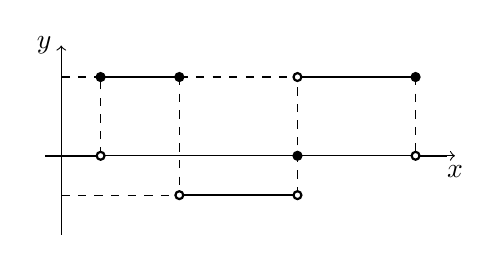
\begin{tikzpicture}
        \draw[->] (-0.2,0) -- (5,0) node[below] {$x$};
        \draw[->] (0,-1) -- (0,1.4) node[left] {$y$};
        \begin{scope}[style = dashed]
            \draw (0,1) -- (0.5,1);
            \draw (1.5,1) -- (3,1);
            \draw (0,-0.5) -- (1.5,-0.5);
            \draw (0.5,0) -- (0.5,1);
            \draw (1.5,1) -- (1.5,-0.5);
            \draw (3,-0.5) -- (3,1);
            \draw (4.5,1) -- (4.5,0);
        \end{scope}
        \begin{scope}[style = thick]
            \draw (-0.2,0) -- (0.5,0);
            \draw (0.5,1) -- (1.5,1);
            \draw (1.5,-0.5) -- (3,-0.5);
            \draw (3,1) -- (4.5,1);
            \draw (4.5,0) -- (4.9,0);
            \draw[fill = white] (0.5,0) circle[radius = 0.05];
            \draw[fill = white] (1.5,-0.5) circle[radius = 0.05];
            \draw[fill = white] (3,-0.5) circle[radius = 0.05];
            \draw[fill = white] (3,1) circle[radius = 0.05];
            \draw[fill = white] (4.5,0) circle[radius = 0.05];
            \draw[fill = black] (0.5,1) circle[radius = 0.05];
            \draw[fill = black] (1.5,1) circle[radius = 0.05];
            \draw[fill = black] (3,0) circle[radius = 0.05];
            \draw[fill = black] (4.5,1) circle[radius = 0.05];
        \end{scope}
    \end{tikzpicture}
    \caption{단순함수의 예시.}
\end{figure}

임의의 단순함수 $f:X\to\mathbb{R}^n$에 대해 이가 갖는 유한개의 서로다른 함숫값을 $a_1,\,\cdots,\,a_k\in\mathbb{R}^n$라 하고 각 $i\leq k$에 대해 $A_i=f^{-1}(a_i)$라 하면 $A_1,\,\cdots,\,A_k$는 가측이고 서로소이며 $\bigsqcup_{i=1}^kA_i=X$이다. 따라서 $f=\sum_{i=1}^ka_i\ind_{A_i}$와 같이 지시함수를 사용하여 이를 나타낼 수 있는데, 이러한 형태를 $f$의 \textbf{표준형(\texttt{standard expression})}이라 한다.

\begin{theorem}\label{thm:measurableFunctionApprox}
    가측공간 $(X,\,\mathcal{A})$에서 정의된 가측함수 $f:X\to\overline{\mathbb{R}}$에 대해 적당한 단순함수 $f_i:X\to\mathbb{R}$의 열 $\{f_i\}$가 존재하여 다음을 만족한다.
    \begin{enumerate}
        \item $f(x)\geq0$인 $x\in X$에 대해서는 $0\leq f_i(x)\uparrow f(x)$이고 $f(x)<0$인 $x\in X$에 대해서는 $0\geq f_i(x)\downarrow f(x)$이다.
        \item 임의의 $x\in X$와 모든 $i\in\mathbb{N}$에 대해 $|f(x)-f_i(x)|<2^{-i}$이거나 $|f_i(x)|=i$이다.
    \end{enumerate}
    한편, 가측함수 $f:X\to\mathbb{R}^n$에 대해서도 적당한 단순함수 $f_i:X\to\mathbb{R}^n$의 열 $\{f_i\}$가 존재하여 $f_i\to f$이다.
\end{theorem}

\begin{proof}
    함수열 $\{f_i\}$를
    \begin{equation*}
        f_i:x\mapsto
        \begin{dcases*}
            -i&$f(x)\leq-i$인 경우\\
            -(j-1)2^{-i}&적당한 $j\leq i2^i$에 대해 $-j2^{-i}<f(x)\leq-(j-1)2^{-i}$인 경우\\
            (j-1)2^{-i}&적당한 $j\leq i2^i$에 대해 $(j-1)2^{-i}\leq f(x)<j2^{-i}$인 경우\\
            i&$f(x)\geq i$인 경우
        \end{dcases*}
    \end{equation*}
    로 정의하면 이는 명백히 단순함수이고 정리의 조건 i, ii를 모두 만족함을 쉽게 보일 수 있다.
    
    한편, 가측함수 $f:X\to\mathbb{R}^n$의 경우에는 각 성분이 단순함수인 함수도 단순함수라는 사실로부터 앞선 결과를 성분별로 적용하기만 하면 된다.
\end{proof}

비록 가측함수는 꽤나 다양한 함수를 포괄하는 개념이지만 모든 가측함수는 단순함수의 열로써 근사가 가능하다는 공통된 성질을 가지고, 이는 이후 \texttt{Lebesgue} 적분론의 전개에 있어 매우 중요한 역할을 하게 될 것이다. 나중에 사용할 가측함수에 관한 몇 가지 개념과 성질을 소개하는 것으로 이번 절을 마치도록 하겠다.

\begin{definition}
    공집합이 아닌 집합 $X$, 가측공간 $(Y,\,\mathcal{B})$에 대해 $\mathcal{F}$를 함수 $f:X\to Y$의 모임이라 할 때, 모든 $f\in\mathcal{F}$가 $\mathcal{A}/\mathcal{B}$-가측이도록 하는 가장 작은 $\sigma$-대수 $\mathcal{A}$를 \textbf{$\mathcal{F}$가 생성하는 $\sigma$-대수($\sigma$-\texttt{algebra generated by} $\mathcal{F}$)}라 하고 $\sigma(\mathcal{F})$로 쓴다.
\end{definition}

\begin{proposition}
    공집합이 아닌 집합 $X$, 가측공간 $(Y,\,\mathcal{B})$에 대해 $\mathcal{F}$를 함수 $f:X\to Y$의 모임이라 하면 이가 생성하는 $\sigma$-대수 $\sigma(\mathcal{F})$는 유일하게 존재한다. 따라서, $\sigma(\mathcal{F})$는 \texttt{well-define}된다.
\end{proposition}

\begin{proof}
    $\sigma(\mathcal{F})$가 존재하기만 한다면, 이의 유일성은 그 정의로부터 자명하다. 존재성의 경우 $\Sigma$를 모든 $f\in\mathcal{F}$가 $\mathcal{A}/\mathcal{B}$-가측이도록 하는 모든 $\sigma$-대수 $\mathcal{A}$의 모임이라 두고 명제 \ref{prop:generatedSigmaAlgebra}의 증명을 그대로 따라가면 된다.
\end{proof}

특히, $\mathcal{F}$가 한원소 집합인 경우에는 $\sigma(\mathcal{F})$의 원소들과 $\sigma(\mathcal{F})/\mathcal{B}_n$-가측인 함수들을 명시적으로 표현할 수 있다.

\begin{theorem}\label{thm:functionGeneratedSigmaAlgebra}
    공집합이 아닌 집합 $X$, 가측공간 $(Y,\,\mathcal{B})$와 함수 $f:X\to Y$에 대해 $\sigma(f)=\{f^{-1}(A)\subseteq X:A\in\mathcal{B}\}$이다.
\end{theorem}

\begin{proof}
    집합족 $\mathcal{C}=\{f^{-1}(A)\subseteq X:A\in\mathcal{B}\}$에 대해 이가 $\sigma$-대수라면 $f$가 $\mathcal{C}/\mathcal{B}$-가측임이 분명하므로 $\sigma(f)\subseteq\mathcal{C}$인 한편, 정의로부터 역의 포함관계는 자명하므로 증명이 끝난다. 따라서 $\mathcal{C}$가 $\sigma$-대수임을 보이는 것으로 충분하다. 우선 $\emptyset = f^{-1}(\emptyset)\in\mathcal{C}$에서 이는 비어있지 않다. 또한, 임의의 $B\in\mathcal{C}$에 대해 적당한 $A\in\mathcal{B}$가 존재하여 $B=f^{-1}(A)$이므로 $B^c=[f^{-1}(A)]^c=f^{-1}(A^c)\in\mathcal{C}$가 되어 $\mathcal{C}$는 여집합에 대해 닫혀있다. 마지막으로 $\mathcal{C}$에 속하는 임의의 집합열 $\{B_i\}$를 생각하면 각 $i\in\mathbb{N}$에 대해 적당한 $A_i\in\mathcal{B}$가 존재하여 $B_i=f^{-1}(A_i)$이므로 $\bigcup_{i=1}^\infty B_i=\bigcup_{i=1}^\infty f^{-1}(A_i)=f^{-1}(\bigcup_{i=1}^\infty A_i)\in\mathcal{C}$가 되어 $\mathcal{C}$는 가산 합집합에 대해서도 닫혀 있고, 곧 이는 $\sigma$-대수이다.
\end{proof}

\begin{theorem}
    공집합이 아닌 집합 $X$에서 정의된 $f:X\to\mathbb{R}^m$에 대해 함수 $g:X\to\mathbb{R}^n$(혹은 $g:X\to\overline{\mathbb{R}}$)가 $\sigma(f)/\mathcal{B}_n$-가측(혹은 $\sigma(f)/\mathcal{B}_1$-가측)일 필요충분조건은 적당한 \texttt{Borel} 함수 $h:\mathbb{R}^m\to\mathbb{R}^n$(혹은 $h:\mathbb{R}^m\to\overline{\mathbb{R}}$)가 존재하여 $g=h\circ f$인 것이다.
\end{theorem}

\begin{proof}
    먼저 충분조건임을 보이기 위해 $g$가 단순함수인 경우를 생각해보자. 단순함수 $g$의 표준형을 $\sum_{i=1}^ka_i\ind_{A_i}$라 하면 각 $i\leq k$에 대해 $A_i\in\sigma(f)$이므로 정리 \ref{thm:functionGeneratedSigmaAlgebra}로부터 적당한 $B_i\in\mathcal{B}_m$가 존재하여 $A_i=f^{-1}(B_i)$이다. 이제 $h=\sum_{i=1}^ka_i\ind_{B_i}$라 하면 이는 명백히 \texttt{Borel} 함수이다. 또한, 각 $i\in\mathbb{N}$와 임의의 $x\in A_i$에 대해 $f(x)\in B_i$이고 $j\ne i$에 대해서는 $f(x)\in B_j$일 수 없으므로 $g=h\circ f$이다. (만약 $f(x)\in B_j$이면 $A_1,\,\cdots,\,A_k$가 서로소라는 표준형의 전제에 모순된다.)

    이제 일반적인 $\sigma(f)/\mathcal{B}_n$-가측함수 $g$를 생각하면 정리 \ref{thm:measurableFunctionApprox}로부터 적당한 단순함수 $g_i:X\to\mathbb{R}^n$의 열 $\{g_i\}$가 존재하여 $g_i\to g$이고 각 $i\in\mathbb{N}$에 대해 $g_i$는 $\sigma(f)/\mathcal{B}_n$-가측이므로 앞선 결과로부터 적당한 \texttt{Borel} 함수 $h_i:\mathbb{R}^m\to\mathbb{R}^n$가 존재하여 $g_i=h_i\circ f$이다. 이제 $A=\{x\in\mathbb{R}^m:\{h_i(x)\}_i\textrm{가 수렴}\}$라 두고 함수 $h$를
    \begin{equation*}
        h:x\mapsto
        \begin{dcases*}
            \lim_{i\to\infty}h_i(x)&$x\in A$인 경우\\
            0&\texttt{ow.}
        \end{dcases*}
    \end{equation*}
    로 정의하면 이는 \texttt{Borel}이고, 임의의 $x\in X$에 대해 $\lim_{i\to\infty}h_i(f(x))=\lim_{i\to\infty}g_i(x)=g(x)$에서 $f(x)\in A$이므로 $g=h\circ f$임을 안다.

    반대로, 필요조건임을 보이는 것은 쉽다. 임의의 $x\in\mathbb{R}^n$에 대해 $h^{-1}((-\infty,\,x])$가 \texttt{Borel}이므로 정리 \ref{thm:functionGeneratedSigmaAlgebra}로부터 $g^{-1}((-\infty,\,x])=f^{-1}(h^{-1}((-\infty,\,x]))\in\sigma(f)$가 되어 $g$는 $\sigma(f)/\mathcal{B}_n$-가측이다.

    한편, 함수 $g:X\to\overline{\mathbb{R}}$의 경우에도 이와 비슷하게 보일 수 있다.
\end{proof}

다음은 측도공간의 완비화와 관련이 있다. 결론부터 말하자면, 측도공간의 완비화는 함수의 가측성을 보존하며, 완비화된 공간에서 가측인 함수는 원래 공간에서의 가측함수에 의해 근사될 수 있다는 것이 다음 정리의 함의이다.

\begin{theorem}\label{thm:measureCompletionApprox}
    측도공간 $(X,\,\mathcal{A},\,\mu)$에서 정의된 함수 $f:X\to\mathbb{R}^n$(혹은 $f:X\to\overline{\mathbb{R}}$)에 대해 다음이 성립한다.
    \begin{enumerate}
        \item 만약 $f$가 $\mathcal{A}/\mathcal{B}_n$-가측(혹은 $\mathcal{A}/\mathcal{B}_1$-가측)이면 이는 $\overline{\mathcal{A}}/\mathcal{B}_n$-가측(혹은 $\overline{\mathcal{A}}/\mathcal{B}_1$-가측)이다.
        \item 만약 $f$가 $\overline{\mathcal{A}}/\mathcal{B}_n$-가측(혹은 $\overline{\mathcal{A}}/\mathcal{B}_1$-가측)이면 적당한 $\mathcal{A}/\mathcal{B}_n$-가측함수 $g:X\to\mathbb{R}^n$(혹은 $\mathcal{A}/\mathcal{B}_1$-가측함수 $g:X\to\overline{\mathbb{R}}$)가 존재하여 $f=g$ (\texttt{ae.})이다.
    \end{enumerate}
\end{theorem}

\begin{proof}
    i. 이는 $\mathcal{A}\subseteq\overline{\mathcal{A}}$에서 자명하다.

    ii. 먼저 $f$가 단순함수인 경우를 생각해보자. 이제 $f$의 표준형을 $f=\sum_{i=1}^ka_i\ind_{A_i}$라 하면 가정으로부터 각 $i\leq k$에 대해 적당한 $B_i\in\mathcal{A}$와 영집합 $N_i\subseteq X$가 존재하여 $A_i=B_i\cup N_i$이다. 그렇다면 함수 $g$를 $g=\sum_{i=1}^ka_i\ind_{B_i}$라 하면 이는 명백히 $\mathcal{A}/\mathcal{B}_n$-가측이고, $\{x\in X:f(x)\ne g(x)\}=\bigcup_{i=1}^k(A_i\setminus B_i)\subseteq\bigcup_{i=1}^kN_i$에서 $\bigcup_{i=1}^kN_i$도 영집합이므로 $f=g$ (\texttt{ae.})이다.

    한편, 일반적인 $\overline{\mathcal{A}}/\mathcal{B}_n$-가측함수 $f$를 생각하면 정리 \ref{thm:measurableFunctionApprox}로부터 적당한 단순함수 $f_i:X\to\mathbb{R}^n$의 열 $\{f_i\}$가 존재하여 $f_i\to f$이고, 앞선 결과로부터 각 $i\in\mathbb{N}$에 대해 적당한 $\mathcal{A}/\mathcal{B}_n$-가측함수 $g_i:X\to\mathbb{R}^n$가 존재하여 $f_i=g_i$ (\texttt{ae.})이다. 이제 각 $i\in\mathbb{N}$에 대해 $N_i=\{x\in X:f_i(x)\ne g_i(x)\}$라 하면 이는 영집합이므로 $N=\bigcup_{i=1}^\infty N_i$도 영집합이어서 적당한 $C\in\mathcal{A}$에 대해 $N\subseteq C$이고 $\mu(C)=0$이다. 이제 임의의 $x\in X\setminus C$에 대해 $g_i(x)\to f(x)$이므로 함수 $g:X\to\mathbb{R}^n$를
    \begin{equation*}
        g:x\mapsto
        \begin{dcases*}
            \lim_{i\to\infty}g_i(x)&$x\in X\setminus C$인 경우\\
            0&\texttt{ow.}
        \end{dcases*}
    \end{equation*}
    로 두면 이는 $\mathcal{A}/\mathcal{B}_n$-가측이고, $f=g$ (\texttt{ae.})임을 안다.

    한편, 함수 $f:X\to\overline{\mathbb{R}}$의 경우에도 이와 비슷하게 보일 수 있다.
\end{proof}

위의 정리의 ii에서 임의의 $\mu$-영집합은 $\overline{\mu}$-영집합이고 그 역도 성립하므로 일부러 어떤 측도를 기준으로 거의 어디서나인지를 나타내지 않았다.

\section{Integration}

이번 절의 전반부에서 우리는 \texttt{Lebesgue} 적분을 총 세 단계에 걸쳐 정의한다. 먼저 첫 번째 단계에서는 음이 아닌 단순함수들에 대해 \texttt{Lebesgue} 적분을 정의한다. 이어지는 두 번째 단계에서는 정리 \ref{thm:measurableFunctionApprox}를 사용하여 \texttt{Lebesgue} 적분의 정의를 음이 아닌 가측함수로 확장한다. 마지막으로 세 번째 단계에서는 함수를 양의 부분과 음의 부분으로 나눔으로써 \texttt{Lebesgue} 적분의 정의를 일반적인 가측함수로 확장하여 \texttt{Lebesgue} 적분의 가장 일반적인 정의를 얻는다. 이렇게 \texttt{Lebesgue} 적분의 정의를 끝마친 이후에는 앞서 언급한 바와 같이 \texttt{Lebesgue} 적분론에서 적분과 극한의 순서를 바꾸는 데 사용되는 유용한 정리들을 살펴보도록 하겠다.

\begin{definition}
    측도공간 $(X,\,\mathcal{A},\,\mu)$에서 정의된 음이 아닌 단순함수 $f:X\to\mathbb{R}^+_0$에 대해 이의 표준형을 $f=\sum_{i=1}^ka_i\ind_{A_i}$라 하면 이때 $\mu$에 대한 $f$의 \textbf{(\texttt{Lebesgue}) 적분(- \texttt{integral})}을 $\int_Xf(x)\,d\mu(x)$ 혹은 간단히 $\int_Xf\,d\mu$로 쓰고 $\int_Xf\,d\mu=\sum_{i=1}^ka_i\mu(A_i)$로 정의한다.
\end{definition}

\begin{proposition}\label{prop:simpleFunctionIntegral}
    측도공간 $(X,\,\mathcal{A},\,\mu)$에 대해 $A_1,\,\cdots,\,A_k\in\mathcal{A}$를 $X=\bigsqcup_{i=1}^kA_i$인 서로소인 집합이라 하자. 이제 $a_1,\,\cdots,\,a_k\geq0$에 대해 함수 $f:X\to\mathbb{R}^+_0$를 $f=\sum_{i=1}^ka_i\ind_{A_i}$라 하면 $\int_Xf\,d\mu=\sum_{i=1}^ka_i\mu(A_i)$이다.
\end{proposition}

\begin{proof}
    양수 $a_1,\,\cdots,\,a_k$ 중에서 서로 같은 값들을 하나만 남기고 제거하여 이를 $b_1,\,\cdots,\,b_l\in\mathbb{R}$라 하고 각 $j\leq l$에 대해 $B_j=f^{-1}(b_j)=\bigsqcup_{i:a_i=b_j}A_i$라 하면 이는 가측이고 $f=\sum_{j=1}^lb_j\ind_{B_j}$이다. 그렇다면 이는 곧 단순함수 $f$의 표준형이므로 \texttt{Lebesgue} 적분의 정의로부터 $\int_Xf\,d\mu=\sum_{j=1}^lb_j\mu(B_j)=\sum_{j=1}^lb_j\mu(\bigsqcup_{i:a_i=b_j}A_i)=\sum_{j=1}^lb_j\sum_{i:a_i=b_j}\mu(A_i)=\sum_{i=1}^ka_i\mu(A_i)$이다.
\end{proof}

위의 명제에서는 $a_1,\,\cdots,\,a_k$가 서로 다르다는 조건이 없으므로 이는 음의 아닌 단순함수에 대한 적분의 정의보다 조금 더 일반적이다. 다음으로 \texttt{Lebesgue} 적분의 기초적인 성질들을 보자.

\begin{proposition}
    측도공간 $(X,\,\mathcal{A},\,\mu)$에서 정의된 음이 아닌 단순함수 $f,\,g:X\to\mathbb{R}^+_0$에 대해 다음이 성립한다.
    \begin{enumerate}
        \item 임의의 $c\geq0$에 대해 $\int_Xcf\,d\mu=c\int_Xf\,d\mu$이다.
        \item $\int_Xf+g\,d\mu=\int_Xf\,d\mu+\int_Xg\,d\mu$.
        \item 만약 $f\leq g$이면 $\int_Xf\,d\mu\leq\int_Xg\,d\mu$이다.
    \end{enumerate}
\end{proposition}

\begin{proof}
    단순함수 $f,\,g$의 표준형을 각각 $f=\sum_{i=1}^ka_i\ind_{A_i},\,g=\sum_{j=1}^lb_j\ind_{B_j}$라 하자.

    i. 함수 $cf=\sum_{i=1}^kca_i\ind_{A_i}$가 음이 아닌 단순함수임이 분명하므로 명제 \ref{prop:simpleFunctionIntegral}로부터 $\int_Xcf\,d\mu=\sum_{i=1}^kca_i\mu(A_i)=c\sum_{i=1}^ka_i\mu(A_i)=c\int_Xf\,d\mu$이다.

    ii. 함수 $f+g=\sum_{i=1}^k\sum_{j=1}^l(a_i+b_j)\ind_{A_i\cap B_j}$가 음이 아닌 단순함수임이 분명하고 $\bigsqcup_{i=1}^k\bigsqcup_{j=1}^l(A_i\cap B_j)=X$이므로 명제 \ref{prop:simpleFunctionIntegral}로부터 $\int_Xf+g\,d\mu=\sum_{i=1}^k\sum_{j=1}^l(a_i+b_j)\mu(A_i\cap B_j)$이다. 한편, $f=\sum_{i=1}^k\sum_{j=1}^la_i\ind_{A_i\cap B_j},\,g=\sum_{i=1}^k\sum_{j=1}^lb_j\ind_{A_i\cap B_j}$로 쓸 수 있으므로 다시 명제 \ref{prop:simpleFunctionIntegral}로부터 $\int_Xf\,d\mu=\sum_{i=1}^k\sum_{j=1}^la_i\mu(A_i\cap B_j)$이고 $\int_Xg\,d\mu=\sum_{i=1}^k\sum_{j=1}^lb_j\mu(A_i\cap B_j)$가 되어 명제가 성립한다.

    iii. 함수 $g-f$가 음이 아닌 단순함수이므로 ii로부터 $\int_Xg\,d\mu=\int_Xg-f\,d\mu+\int_Xf\,d\mu\geq\int_Xf\,d\mu$이다.
\end{proof}

\begin{corollary}
    측도공간 $(X,\,\mathcal{A},\,\mu)$와 $A_1,\,\cdots,\,A_k\in\mathcal{A},\,a_1,\,\cdots,\,a_k\geq0$에 대해 함수 $f:X\to\mathbb{R}^+_0$를 $f=\sum_{i=1}^ka_i\ind_{A_i}$라 하면 $\int_Xf\,d\mu=\sum_{i=1}^ka_i\mu(A_i)$이다.
\end{corollary}

\begin{proof}
    이는 $\int_Xf\,d\mu=\sum_{i=1}^ka_i\int_X\ind_{A_i}\,d\mu=\sum_{i=1}^ka_i\mu(A_i)$에서 자명하다.
\end{proof}

위의 따름정리에서는 $A_1,\,\cdots,\,A_k$가 서로소일 필요도, $X$의 덮개일 필요도 없다. 따라서 이는 명제 \ref{prop:simpleFunctionIntegral}의 결과에서 한 발짝 더 나아간 결과이다. 이제 두 번째 단계로 넘어가자.

\begin{definition}
    측도공간 $(X,\,\mathcal{A},\,\mu)$에서 정의된 음이 아닌 가측함수 $f:X\to\overline{\mathbb{R}}^+_0$에 대해 $\mu$에 대한 $f$의 \textbf{(\texttt{Lebesgue}) 적분(- \texttt{integral})}을 $\int_Xf(x)\,d\mu(x)$ 혹은 간단히 $\int_Xf\,d\mu$로 쓰고
    \begin{equation*}
        \int_Xf\,d\mu=\sup\bigg\{\int_Xg\,d\mu\in\overline{\mathbb{R}}:\textrm{함수 $g:X\to\mathbb{R}^+_0$는 $g\leq f$인 음이 아닌 단순함수}\bigg\}
    \end{equation*}
    로 정의한다.
\end{definition}

정리 \ref{thm:measurableFunctionApprox}로부터 임의의 음이 아닌 가측함수는 이로 점별수렴하는 음이 아닌 함수열을 가지므로 위의 정의는 \texttt{well-define}되어 있다. 하지만, 이런 정의를 직접 사용하는 것은 그다지 편리하지 않으므로 이를 대신할 정리를 소개한다.

\begin{lemma}
    측도공간 $(X,\,\mathcal{A},\,\mu)$와 $A\in\mathcal{A}$에 대해 음이 아닌 단순함수 $f_i:X\to\mathbb{R}^+_0$의 열 $\{f_i\}$가 증가하고 어떤 $M\geq0$과 모든 $x\in A$에 대해 $\lim_{i\to\infty}f_i(x)\geq M$을 만족한다고 하면 $\lim_{i\to\infty}\int_Xf_i\ind_{A}\,d\mu\geq M\mu(A)$이다.
\end{lemma}

\begin{proof}
    만약 $M=0$이거나 $\mu(A)=0$이면 보조정리가 자명하므로 $M,\,\mu(A)>0$라 하자. 또한, $\{\int_Xf_i\ind_A\,d\mu\}_i$가 증가하므로 만약 이가 위로 유계가 아니라면 이번에도 보조정리가 자명하여 $\{\int_Xf_i\ind_A\,d\mu\}$가 위로 유계라 하자. 그렇다면 \texttt{MSP}로부터 이는 수렴한다. 이제 임의의 양수 $a<M$를 택하고 집합열 $\{A_i\}$를 $A_i=f_i^{-1}([a,\,\infty))\cap A$로 두면 이는 가측이고 $A_i\uparrow A$이다. 따라서 정리 \ref{thm:monoSeriesMeasure}의 i로부터 $\mu(A_i)\uparrow\mu(A)$이고, 곧 임의의 $b<\mu(A)$를 택하면 적당한 $i_0\in\mathbb{N}$가 존재하여 임의의 $i\geq i_0$에 대해 $\mu(A_i)>b$이다. 이상의 결과로부터 임의의 $i\geq i_0$에 대해 $\int_Xf_i\ind_A\,d\mu\geq\int_Xf_i\ind_{A_i}\,d\mu\geq\int_Xa\ind_{A_i}\,d\mu=a\mu(A_i)>ab$가 성립하여 $\lim_{i\to\infty}\int_Xf_i\ind_{A}\,d\mu\geq M\mu(A)$임을 안다.
\end{proof}

\begin{lemma}
    측도공간 $(X,\,\mathcal{A},\,\mu)$에서 정의된 음이 아닌 단순함수 $f:X\to\mathbb{R}^+_0$에 대해 음이 아닌 단순함수 $g_i:X\to\mathbb{R}^+_0$의 열 $\{g_i\}$가 증가하고 $\lim_{i\to\infty}g_i\geq f$를 만족한다면 $\lim_{i\to\infty}\int_Xg_i\,d\mu\geq\int_Xf\,d\mu$이다.
\end{lemma}

\begin{proof}
    단순함수 $f$의 표준형을 $f=\sum_{j=1}^ka_j\ind_{A_j}$라 하면 임의의 $j\leq k$와 임의의 $x\in A_j$에 대해 $\lim_{i\to\infty}g_i(x)\geq a_j$이므로 위의 보조정리로부터 $\lim_{i\to\infty}\int_Xg_i\ind_{A_j}\,d\mu\geq a_j\mu(A_j)$이다. 한편, 각 $i\in\mathbb{N}$에 대해 $\int_Xg_i\,d\mu=\int_Xg_i\sum_{j=1}^k\ind_{A_j}\,d\mu=\sum_{j=1}^k\int_Xg_i\ind_{A_j}\,d\mu$이므로 $\lim_{i\to\infty}\int_Xg_i\,d\mu=\sum_{j=1}^k\lim_{i\to\infty}\int_Xg_i\ind_{A_j}\,d\mu\geq\sum_{j=1}^ka_j\mu(A_j)=\int_Xf\,d\mu$를 얻는다.
\end{proof}

\begin{theorem}\label{thm:approxIntegral}
    측도공간 $(X,\,\mathcal{A},\,\mu)$에서 정의된 음이 아닌 가측함수 $f:X\to\overline{\mathbb{R}}^+_0$에 대해 $f_i\uparrow f$인 임의의 음이 아닌 단순함수 $f_i:X\to\mathbb{R}^+_0$의 열 $\{f_i\}$를 생각하면 $\int_Xf_i\,d\mu\uparrow\int_Xf\,d\mu$이다.
\end{theorem}

\begin{proof}
    수열 $\{\int_Xf_i\,d\mu\}_i$가 증가하므로 이는 수렴하거나 $\infty$로 발산하는데, 후자의 경우 $\int_Xf\,d\mu=\infty$가 되어 정리가 자명하므로 $\{\int_Xf_i\,d\mu\}$가 수렴한다고 가정하자. 그렇다면 $\{\int_Xf_i\,d\mu\}$는 $\int_Xf\,d\mu$에 의해 위로 유계이므로 $\lim_{i\to\infty}\int_Xf_i\,d\mu\leq\int_Xf\,d\mu$이다. 한편, $g\leq f$인 임의의 음이 아닌 단순함수 $g:X\to\mathbb{R}^+_0$에 대해 $f_i\uparrow f\geq g$이므로 위의 보조정리로부터 $\lim_{i\to\infty}\int_X f_i\,d\mu\geq\int_Xg\,d\mu$이고, 곧 $\lim_{i\to\infty}\int_X f_i\,d\mu\geq\int_Xf\,d\mu$가 되어 이를 앞선 결과와 합하면 $\int_Xf_i\,d\mu\uparrow\int_Xf\,d\mu$를 얻는다.
\end{proof}

이제 마지막 단계이다.

\begin{definition}\label{def:integral}
    측도공간 $(X,\,\mathcal{A},\,\mu)$에서 정의된 음이 아닌 가측함수 $f:X\to\overline{\mathbb{R}}^+_0$에 대해 $\int_Xf\,d\mu<\infty$이면 이때의 $f$를 \textbf{($\mu$-\texttt{Lebesgue}) 적분가능(- \texttt{integrable})}하다고 한다. 나아가, 일반적인 가측함수 $f:X\to\overline{\mathbb{R}}$에 대해 $f_\pm$이 모두 적분가능하면 이때의 $f$를 \textbf{($\mu$-\texttt{Lebesgue}) 적분가능(- \texttt{integrable})}하다고 한다. 그리고 이때 $\mu$에 대한 $f$의 \textbf{(\texttt{Lebesgue}) 적분(- \texttt{integral})}을 $\int_Xf(x)\,d\mu(x)$ 혹은 간단히 $\int_Xf\,d\mu$로 쓰고 $\int_Xf\,d\mu=\int_Xf_+\,d\mu-\int_Xf_-\,d\mu$로 정의한다. 여기서 $f_\pm$은 각각 $f$의 양의 부분과 음의 부분을 의미하는 것으로 각각 $f_\pm=(|f|\pm f)/2$로 정의된다.
\end{definition}

\begin{figure}[!ht]
    \centering
    \subfigure{
    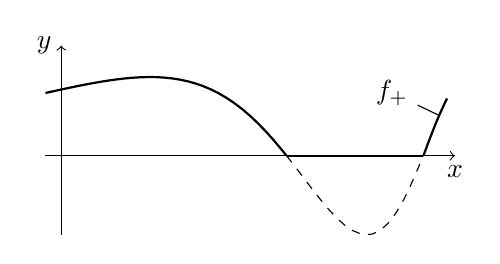
\begin{tikzpicture}
        \draw[->] (-0.2,0) -- (5,0) node[below] {$x$};
        \draw[->] (0,-1) -- (0,1.4) node[left] {$y$};
        \draw[style = dashed] plot[smooth, tension = 1] coordinates {(2.86182,0) (2.9,-0.0483218) (3,-0.177577) (3.1,-0.308885) (3.2,-0.439505) (3.3,-0.566151) (3.4,-0.684998) (3.5,-0.791713) (3.6,-0.881535) (3.7,-0.94941) (3.8,-0.990193) (3.9,-0.998922) (4,-0.971185) (4.1,-0.903564) (4.2,-0.794163) (4.3,-0.64319) (4.4,-0.453553) (4.5,-0.231421) (4.6,0)};
        \begin{scope}[style = thick]
            \draw plot[smooth, tension = 1] coordinates {(-0.2,0.797486) (-0.1,0.819644) (0,0.841471) (0.1,0.862814) (0.2,0.883502) (0.3,0.903341) (0.4,0.922115) (0.5,0.93958) (0.6,0.95547) (0.7,0.969487) (0.8,0.981305) (0.9,0.990566) (1,0.996883) (1.1,0.999836) (1.2,0.998975) (1.3,0.99382) (1.4,0.983866) (1.5,0.968584) (1.6,0.947432) (1.7,0.919857) (1.8,0.88531) (1.9,0.843258) (2,0.793203) (2.1,0.734701) (2.2,0.667386) (2.3,0.591003) (2.4,0.505444) (2.5,0.410781) (2.6,0.30732) (2.7,0.195643) (2.8,0.0766632) (2.86182,0)};
            \draw (2.86182,0) -- (4.6,0);
            \draw plot[smooth, tension = 1] coordinates {(4.6,0) (4.7,0.267039) (4.8,0.512225) (4.9,0.728508)};
        \end{scope}
        \node (f) at (4.2,0.8) {$f_+$};
        \draw (4.8,0.512225) -- (f);
    \end{tikzpicture}
    }
    \qquad
    \subfigure{
    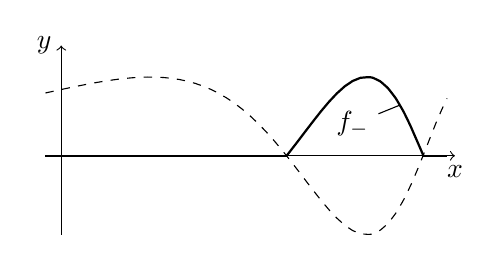
\begin{tikzpicture}
        \draw[->] (-0.2,0) -- (5,0) node[below] {$x$};
        \draw[->] (0,-1) -- (0,1.4) node[left] {$y$};
        \draw[style = dashed] plot[smooth, tension = 1] coordinates {(-0.2,0.797486) (-0.1,0.819644) (0,0.841471) (0.1,0.862814) (0.2,0.883502) (0.3,0.903341) (0.4,0.922115) (0.5,0.93958) (0.6,0.95547) (0.7,0.969487) (0.8,0.981305) (0.9,0.990566) (1,0.996883) (1.1,0.999836) (1.2,0.998975) (1.3,0.99382) (1.4,0.983866) (1.5,0.968584) (1.6,0.947432) (1.7,0.919857) (1.8,0.88531) (1.9,0.843258) (2,0.793203) (2.1,0.734701) (2.2,0.667386) (2.3,0.591003) (2.4,0.505444) (2.5,0.410781) (2.6,0.30732) (2.7,0.195643) (2.8,0.0766632) (2.9,-0.0483218) (3,-0.177577) (3.1,-0.308885) (3.2,-0.439505) (3.3,-0.566151) (3.4,-0.684998) (3.5,-0.791713) (3.6,-0.881535) (3.7,-0.94941) (3.8,-0.990193) (3.9,-0.998922) (4,-0.971185) (4.1,-0.903564) (4.2,-0.794163) (4.3,-0.64319) (4.4,-0.453553) (4.5,-0.231421) (4.6,0.0133526) (4.7,0.267039) (4.8,0.512225) (4.9,0.728508)};
        \begin{scope}[style = thick]
            \draw plot[smooth, tension = 1] coordinates {(2.86182,0) (2.9,0.0483218) (3,0.177577) (3.1,0.308885) (3.2,0.439505) (3.3,0.566151) (3.4,0.684998) (3.5,0.791713) (3.6,0.881535) (3.7,0.94941) (3.8,0.990193) (3.9,0.998922) (4,0.971185) (4.1,0.903564) (4.2,0.794163) (4.3,0.64319) (4.4,0.453553) (4.5,0.231421) (4.6,0)};
            \draw (-0.2,0) -- (2.86182,0);
            \draw (4.6,0) -- (4.9,0);
        \end{scope}
        \node (f) at (3.7,0.4) {$f_-$};
        \draw (4.3,0.64319) -- (f);
    \end{tikzpicture}
    }
    \caption{함수 $f$ (파선)에 대한 $f_+$ (왼쪽)와 $f_-$ (오른쪽)의 그래프.}
\end{figure}

\begin{definition}
    측도공간 $(X,\,\mathcal{A},\,\mu)$에서 정의된 가측함수 $f:X\to\overline{\mathbb{R}}$와 $A\in\mathcal{A}$에 대해 함수 $f\ind_A$가 적분가능하면 이때의 $f$를 $A$ 위에서 \textbf{($\mu$-\texttt{Lebesgue}) 적분가능(\texttt{integrable})}하다고 한다. 그리고 이때 $\mu$에 대한 $f$의 \textbf{$A$에서의 (\texttt{Lebesgue}) 적분(- \texttt{integral over} $A$)}을 $\int_Af(x)\,d\mu(x)$ 혹은 간단히 $\int_Af\,d\mu$로 쓰고 $\int_Af\,d\mu=\int_Xf\ind_A\,d\mu$로 정의한다.
\end{definition}

\texttt{Lebesgue} 적분의 정의가 끝났으니 이제 이의 성질들을 알아보도록 하자. 표기의 편의와 간결한 논의를 위해 대부분의 명제나 정리들에서 적분 영역이 전체 공간 $X$로 주어져 있지만 임의의 가측집합 $A\subseteq X$에 대해 $f$ 대신 $f\ind_A$를 생각함으로써 이들을 임의의 가측집합을 적분 영역으로 갖는 경우로 자명하게 일반화할 수 있다.

\begin{theorem}\label{thm:integralProperty}
    측도공간 $(X,\,\mathcal{A},\,\mu)$에서 정의된 음이 아닌 가측함수 $f,\,g:X\to\overline{\mathbb{R}}^+_0$와 $A,\,B\in\mathcal{A}$에 대해 다음이 성립한다.
    \begin{enumerate}
        \item 임의의 $c\geq0$에 대해 $\int_Xcf\,d\mu=c\int_Xf\,d\mu$이다.
        \item $\int_Xf+g\,d\mu=\int_Xf\,d\mu+\int_Xg\,d\mu$.
        \item 만약 $f\leq g$이면 $\int_Xf\,d\mu\leq\int_Xg\,d\mu$이다.
        \item 만약 $A\subseteq B$이면 $\int_Af\,d\mu\leq\int_Bf\,d\mu$이다.
    \end{enumerate}
    한편, 적분가능한 함수 $f,\,g:X\to\overline{\mathbb{R}}$에 대해서도 iv를 제외한 나머지 성질들이 성립한다. 다만, i의 경우 더 이상 $c\geq0$의 조건이 요구되지 않으며, $cf$와 $f+g$의 적분가능이 보장된다.
    \begin{enumerate}
        \item[i$^\circ$.] 임의의 $c\in\overline{\mathbb{R}}$에 대해 $cf$가 적분가능하고 $\int_Xcf\,d\mu=c\int_Xf\,d\mu$이다.
        \item[ii$^\circ$.] 함수 $f+g$가 적분가능하고 $\int_Xf+g\,d\mu=\int_Xf\,d\mu+\int_Xg\,d\mu$이다.\footnotemark
    \end{enumerate}
    나아가 이 경우, 음이 아닌 가측함수 $f:X\to\overline{\mathbb{R}}^+_0$에 대해서는 자명한 다음 성질도 성립한다.
    \begin{enumerate}
        \item[v.] $|\int_Xf\,d\mu|\leq\int_X|f|\,d\mu$.
    \end{enumerate}
\end{theorem}

\begin{proof}
    정리 \ref{thm:measurableFunctionApprox}로부터 음이 아닌 단순함수 $f_i,\,g_i:X\to\mathbb{R}^+_0$의 열 $\{f_i\},\,\{g_i\}$가 존재하여 $f_i\uparrow f,\,g_i\uparrow g$이고, 그렇다면 정리 \ref{thm:approxIntegral}로부터 $\int_Xf_i\,d\mu\uparrow\int_Xf\,d\mu,\,\int_xg_i\,d\mu\uparrow\int_Xg\,d\mu$이다.

    i. 함수열 $\{cf_i\}$ 음이 아닌 단순함수열로서 $cf_i\uparrow cf$임이 분명하므로 정리 \ref{thm:approxIntegral}로부터 $\int_Xcf\,d\mu=\lim_{i\to\infty}\int_Xcf_i\,d\mu=c\lim_{i\to\infty}\int_Xf_i\,d\mu=c\int_Xf\,d\mu$이다.

    ii. 함수열 $\{f_i+g_i\}$가 음이 아닌 단순함수열로서 $f_i+g_i\uparrow f+g$임이 분명하므로 정리 \ref{thm:approxIntegral}로부터 $\int_Xf+g\,d\mu=\lim_{i\to\infty}\int_Xf_i+g_i\,d\mu=\lim_{i\to\infty}\int_Xf_i\,d\mu+\lim_{i\to\infty}\int_Xg_i\,d\mu=\int_Xf\,d\mu+\int_Xg\,d\mu$이다.

    iii. 상수 함수 $h=0$은 $g-f\geq h$인 음이 아닌 단순함수로 볼 수 있으므로 정의로부터 $\int_Xg-f\,d\mu\geq0$이고, 곧 ii로부터 $\int_Xg\,d\mu=\int_Xg-f\,d\mu+\int_Xf\,d\mu\geq\int_Xf\,d\mu$이다.

    iv. 이는 $f\ind_A\leq f\ind_B$와 iii으로부터 자명하다.

    한편, 적분가능한 함수 $f,\,g:X\to\overline{\mathbb{R}}$의 경우에는 이를 각각 양과 음의 부분으로 나누어 앞선 결과를 적용하면 된다. 특히 i$^\circ$의 경우 $c\geq0$인 경우와 $c<0$인 경우를 나누어 생각하면 된다.

    v. 이는 $-|f|\leq f\leq|f|$와 iii으로부터 $-\int_X|f|\,d\mu\leq\int_Xf\,d\mu\leq\int_X|f|\,d\mu$이므로 자명하다.
\end{proof}

\begin{theorem}\label{thm:integralFinite}
    측도공간 $(X,\,\mathcal{A},\,\mu)$에서 정의된 가측함수 $f:X\to\overline{\mathbb{R}}$와 $A,\,B\in\mathcal{A}$에 대해 다음이 성립한다.
    \begin{enumerate}
        \item 함수 $f$가 적분가능할 필요충분조건은 $|f|$가 적분가능한 것이다.
        \item 만약 $f$가 적분가능하면 이는 거의 어디서나 유한하다.
        \item 만약 $A\subseteq B$이고 $f$가 $B$ 위에서 적분가능하면 이는 $A$ 위에서도 적분가능하다.
    \end{enumerate}
\end{theorem}

\begin{proof}
    i. 정의로부터 $|f|$가 적분가능하다는 것은 $\int_X|f|\,d\mu=\int_Xf_+\,d\mu+\int_Xf_-\,d\mu<\infty$인 것과 동치이고, 이는 다시 $f_+,\,f_-$가 적분가능하다는 것과 동치이므로 곧 정의로부터 $f$가 적분가능하다는 것과 동치이다.

    ii. 우선 $\{\pm\infty\}$가 닫혀있으므로 \texttt{Borel}이고, 따라서 $N=f^{-1}(\pm\infty)$이 가측이다. 그런데 만약 $\mu(N)>0$이라면 $\int_X|f|\,d\mu\geq\int_N|f|\,d\mu=\infty$에서 $f$가 적분가능하다는 가정에 모순되므로 $N$은 영집합이고, 곧 명제가 성립한다.

    iii. i로부터 $\int_A|f|\,d\mu\leq\int_B|f|\,d\mu<\infty$가 되어 이는 자명하다.
\end{proof}

\begin{theorem}\label{thm:zeroAeIntegral}
    측도공간 $(X,\,\mathcal{A},\,\mu)$에서 정의된 가측함수 $f:X\to\overline{\mathbb{R}}$에 대해 다음이 성립한다.
    \begin{enumerate}
        \item 만약 $f=0$ (\texttt{ae.})이면 이는 적분가능하고 $\int_Xf\,d\mu=0$이다.
        \item 만약 $f$가 적분가능하고 거의 어디서나 음이 아니며 $\int_Xf\,d\mu=0$이면 $f=0$ (\texttt{ae.})이다.
    \end{enumerate}
\end{theorem}

\begin{proof}
    i. 먼저 $f$가 음이 아닌 경우를 생각하고 $f\geq g$인 임의의 음이 아닌 단순함수 $g:X\to\mathbb{R}^+_0$를 택하여 이의 표준형을 $g=\sum_{i=1}^ka_i\ind_{A_i}$라 하자. 그렇다면 $g=0$ (\texttt{ae.})이므로 \texttt{WLOG}, $a_1=0$이라 한다면 각 $1<i\leq k$에 대해 $\mu(A_i)=0$이 되어 $\int_Xg\,d\mu=\sum_{i=1}^ka_i\mu(A_i)=0$에서 $\int_Xf\,d\mu=0$이다. 이제 일반적인 가측함수 $f$에 대해서 $f_+=f_-=0$ (\texttt{ae.})이므로 앞선 결과로부터 $\int_xf\,d\mu=\int_Xf_+\,d\mu-\int_Xf_-\,d\mu=0$이다.

    ii. 먼저 $f$가 음이 아닌 경우를 생각하고 모순을 유도하기 위해 $f=0$ (\texttt{ae.})가 아니라 가정하자. 이제 집합열 $\{A_i\}$를 $A_i:=f^{-1}((1/i,\,\infty])$로 두면 이는 가측이고 곧 $\bigcup_{i=1}^\infty A_i=f^{-1}(\bigcup_{i=1}^\infty(1/i,\,\infty])=f^{-1}((0,\,\infty])$도 가측이 되어 가정으로부터 양의 측도를 가진다. 나아가 $A_i\uparrow f^{-1}((0,\,\infty])$이므로 정리 \ref{thm:monoSeriesMeasure}의 i로부터 $\mu(A_i)\uparrow\mu(f^{-1}((0,\,\infty]))>0$이 되어 $\mu(A_{i_0})>0$인 적당한 $i_0\in\mathbb{N}$가 존재한다. 그러나, $g=\ind_{A_{i_0}}/i_0$라 하면 이가 $f\geq g$인 음이 아닌 단순함수이므로 $\int_Xf\,d\mu\geq\int_Xg\,d\mu=\mu(A_{i_0})/i_0>0$의 모순이 발생한다. 따라서 $f=0$ (\texttt{ae.})이다. 이제 일반적인 가측함수 $f$에 대해 가정으로부터 $f_-=0$ (\texttt{ae.})이므로 i에서 $\int_Xf_+\,d\mu=\int_Xf_-\,d\mu=0$이고, 곧 앞선 결론으로부터 $f_+=0$ (\texttt{ae.})가 성립하여 $f=0$ (\texttt{ae.})임을 안다.
\end{proof}

\begin{corollary}\label{cor:zeroAeIntegral}
    측도공간 $(X,\,\mathcal{A},\,\mu)$에서 정의된 음이 아닌 가측함수 $f,\,g:X\to\overline{\mathbb{R}}^+_0$에 대해 다음이 성립한다.
    \begin{enumerate}
        \item 만약 $N\in\mathcal{A}$이 영집합이면 $f$는 $N$ 위에서 적분가능하며 $\int_Nf\,d\mu=0$이다.
        \item 만약 $f=g$ (\texttt{ae.})이면 $\int_Xf\,d\mu=\int_Xg\,d\mu$이다.
        \item 만약 $\{x\in X:f(x)>0\}$이 양의 측도를 가지면 $\int_Xf\,d\mu>0$이다.
    \end{enumerate}
    한편, 적분가능한 함수 $f:X\to\overline{\mathbb{R}}$와 일반적인 가측함수 $g:X\to\overline{\mathbb{R}}$에 대해서도 iii을 제외한 나머지 성질들이 성립한다. 특히 ii의 경우 $g$의 적분가능성까지 보장된다.
    \begin{enumerate}
        \item[ii$^\circ$] 만약 $f=g$ (\texttt{ae.})이면 $g$도 적분가능하고 $\int_Xf\,d\mu=\int_Xg\,d\mu$이다.
    \end{enumerate}
\end{corollary}

\begin{proof}
    i. 이는 $f\ind_N=0$ (\texttt{ae.})에서 정리 \ref{thm:zeroAeIntegral}의 i로부터 자명하다.

    ii. 가정으로부터 적당한 영집합 $N\in\mathcal{A}$가 존재하여 $X\setminus N$에서 $f=g$이고, i로부터 $\int_Xf\,d\mu=\int_{X\setminus N}f\,d\mu+\int_Nf\,d\mu=\int_{X\setminus N}g\,d\mu=\int_{X\setminus N}g\,d\mu+\int_Ng\,d\mu=\int_Xg\,d\mu$이다.

    iii. 만약 $\int_Xf\,d\mu=0$이면 정리 \ref{thm:zeroAeIntegral}의 ii로부터 $f=0$ (\texttt{ae.})의 모순이 발생하므로 명제가 자명하다.

    한편, 적분가능한 함수 $f:X\to\overline{\mathbb{R}}$와 일반적인 가측함수 $g:X\to\overline{\mathbb{R}}$의 경우에는 이를 각각 양과 음의 부분으로 나누어 앞선 결과를 적용하면 된다.
\end{proof}

이제 이번 절의 후반부로서 \texttt{Lebesgue} 적분과 극한이 서로 어떻게 상호작용하는지에 대해 알아보도록 하자. 이러한 상호작용을 규정하는 정리들을 흔히 `수렴정리'라 부른다. 아쉽게도, 어느 경우에나 항상 사용할 수 있는 일반적인 수렴정리는 존재하지 않는다. 곧 각각의 수렴정리는 나름의 조건을 요구하는데, 수렴정리를 적용하기 전에 이러한 조건을 반드시 확인해야 한다.\footnotemark 첫 번째로 살펴볼 수렴정리는 함수열이 음이 아니며 증가할 것을 요구한다.

\begin{theorem}[Monotone convergence theorem]
    측도공간 $(X,\,\mathcal{A},\,\mu)$에서 정의된 음이 아닌 가측함수 $f_i:X\to\overline{\mathbb{R}}^+_0$의 열 $\{f_i\}$가 증가하며 적당한 음이 아닌 가측함수 $f:X\to\overline{\mathbb{R}}^+_0$에 대해 $f_i\uparrow f$ (\texttt{ae.})라 하면 $\int_Xf_i\,d\mu\uparrow\int_Xf\,d\mu$이다.
\end{theorem}

\begin{proof}
    먼저 $f_i\uparrow f$인 경우를 생각하면 수열 $\{\int_Xf_i\,d\mu\}_i$가 증가하고 $\int_Xf\,d\mu$에 의해 위로 유계이므로 $\lim_{i\to\infty}\int_Xf_i\,d\mu\leq\int_Xf\,d\mu$이다. 따라서 역의 대소관계만 보인다면 이 경우에 대해서는 증명이 끝난다. 이를 위해 각 $i\in\mathbb{N}$에 대해 음이 아닌 단순함수 $g_{ij}:X\to\mathbb{R}^+_0$의 열 $\{g_{ij}\}_j$를 정리 \ref{thm:measurableFunctionApprox}의 증명에서의 함수열과 같이 잡고 함수열 $\{h_i\}$를 $h_i:=g_{ii}$로 두자. 이제 $h_i\uparrow f$임을 보이기 위해 $\{h_i\}$가 증가한다는 것과 $f$로 수렴한다는 것을 주장한다.

    함수열 $\{h_i\}$가 증가한다는 점은 경우를 나누어 하나하나 확인해봄으로써 어렵지 않게 알 수 있다. 우선 임의의 $x\in X$와 임의의 $i\in\mathbb{N}$를 택하면 우리가 생각해야 할 경우는 다음의 네 가지이다.
    \begin{enumerate}
        \item $f_i(x)\geq i$ 이고 $f_{i+1}(x)\geq i+1$인 경우.
        \item $i\leq f_i(x)\leq f_{i+1}(x)<i+1$인 경우.
        \item $f_i(x)<i$ 이고 $f_{i+1}(x)\geq i+1$인 경우.
        \item $f_i(x)\leq f_{i+1}(x)<i$인 경우.
    \end{enumerate}
    연습삼아 처음 두 개의 경우에 대해서만 확인해보면, i의 경우에는 $h_{i+1}(x)=i+1\geq i=h_i(x)$에서 자명하다. 한편, ii의 경우에는 적당한 자연수 $j\leq(i+1)2^{i+1}$가 존재하여 $(j-1)2^{-i-1}\leq f(x)<j2^{-i-1}$인데, 이는 $i2^{i+1}<j\leq(i+1)2^{i+1}$임을 뜻하므로 곧 $h_{i+1}(x)=(j-1)2^{-i-1}\geq i=h_i(x)$에서 이 또한 자명하다. 남은 두 경우에 대해서도 이와 같이 쉽게 따져볼 수 있으므로 $\{h_i\}$는 증가함을 안다.

    다음으로 $h_i\uparrow f$임을 확인해보자. 일단, 임의의 $x\in X$를 택하면 임의의 $i\in\mathbb{N}$에 대해 $|f_i(x)-h_i(x)|<2^{-i}$이거나 $h_i(x)=i$이다. 여기서 만약 무한히 많은 $i\in\mathbb{N}$에 대해 $h_i(x)=i$라면 $f_i(x)\to\infty$에서 $f(x)=\infty$인 한편, $h_i(x)\to\infty$이므로 $h_i\uparrow f$이다. 만약 그렇지 않다면 충분히 큰 $i\in\mathbb{N}$에 대해 $|f_i(x)-h_i(x)|<2^{-i}$이고, 곧 $h_i(x)\uparrow f(x)$임이 분명하다.

    이제 $h_i\uparrow f$임을 알았으므로 정리 \ref{thm:approxIntegral}로부터 $\int_Xh_i\,d\mu\uparrow\int_Xf\,d\mu$이고 $\{h_i\}$의 구성으로부터 모든 $i\in\mathbb{N}$에 대해  $h_i\leq f_i$이므로 $\int_Xf\,d\mu\leq\lim_{i\to\infty}f_i\,d\mu$에서 증명이 끝난다.

    한편, $f_i\uparrow f$ (\texttt{ae.})인 경우에 대해서는 $N=\{x\in X:f_i(x)\not\to f(x)\}$을 생각하면 이가 영집합이고 정리 \ref{thm:limitMeasurable}의 iv로부터 가측이다. 이제 함수 $g_i:X\to\overline{\mathbb{R}}^+_0$의 열 $\{g_i\}$와 함수 $g:X\to\overline{\mathbb{R}}^+_0$를 각각 $g_i=f_i\ind_{X\setminus N},\,g=f\ind_{X\setminus N}$과 같이 정의하면 $\{g_i\}$는 음이 아닌 가측함수의 열로, 증가하고 $g_i\uparrow g$이다. 그렇다면 앞서 얻은 결과로부터 $\int_Xg_i\,d\mu\uparrow\int_Xg\,d\mu$임을 바로 알 수 있고, 곧 모든 $i\in\mathbb{N}$에 대해 $f_i=g_i$ (\texttt{ae.})이며 $f=g$ (\texttt{ae.})이므로 따름정리 \ref{cor:zeroAeIntegral}의 ii로부터 $\int_Xf_i\,d\mu\uparrow\int_Xf\,d\mu$를 얻는다.
\end{proof}

두 번째 수렴정리는 함수열이 음이 아닐 것만을 요구하는 대신, 등호가 아닌 부등호의 관계만 보장한다.

\begin{theorem}[Fatou's lemma]
    측도공간 $(X,\,\mathcal{A},\,\mu)$에서 정의된 음이 아닌 가측함수 $f_i:X\to\overline{\mathbb{R}}^+_0$의 열 $\{f_i\}$에 대해 $\liminf_{i\to\infty}\int_Xf_i\,d\mu\geq\int_X\liminf_{i\to\infty}f_i\,d\mu$이다.
\end{theorem}

\begin{proof}
    함수열 $\{g_i\}$를 $g_i:=\inf_{j\geq i}f_j$로 두면 이는 증가하는 함수열로 정리 \ref{thm:limitMeasurable}의 i로부터 각 $g_i$가 가측이므로 \texttt{MCT}에서 $\lim_{i\to\infty}\int_Xg_i\,d\mu=\int_X\lim_{i\to\infty}g_i\,d\mu=\int_X\sup_{i\in\mathbb{N}}\inf_{j\geq i}f_j\,d\mu=\int_X\liminf_{i\to\infty}f_i\,d\mu$이다. 그렇다면 모든 $i\in\mathbb{N}$에 대해 $g_i\leq f_i$이므로 $\liminf_{i\to\infty}\int_Xf_i\,d\mu\geq\liminf_{i\to\infty}\int_Xg_i\,d\mu=\lim_{i\to\infty}\int_Xg_i\,d\mu=\int_X\liminf_{i\to\infty}f_i\,d\mu$이다.
\end{proof}

마지막 수렴정리는 그 이름에서 알 수 있듯이 `지배'라는 독특한 조건을 요구한다. 즉, 함수열이 어떤 적분가능한 함수에 의해 지배되어야 한다.

\begin{theorem}[Lebesgue's dominated convergence theorem]
    측도공간 $(X,\,\mathcal{A},\,\mu)$에서 정의된 가측함수 $f_i:X\to\overline{\mathbb{R}}$의 열 $\{f_i\}$와 가측함수 $f:X\to\overline{\mathbb{R}}$에 대해 $f_i\to f$ (\texttt{ae.})라 하자. 또한, 어떤 적분가능한 함수 $g:X\to\overline{\mathbb{R}}^+_0$가 존재하여 모든 $i\in\mathbb{N}$에 대해 $|f_i|\leq g$이면 각 $f_i$와 $f$는 적분가능하고 $\int_Xf_i\,d\mu\to\int_Xf\,d\mu$이다.
\end{theorem}

\begin{figure}[!ht]
    \sidecaption[b]
    \centering
    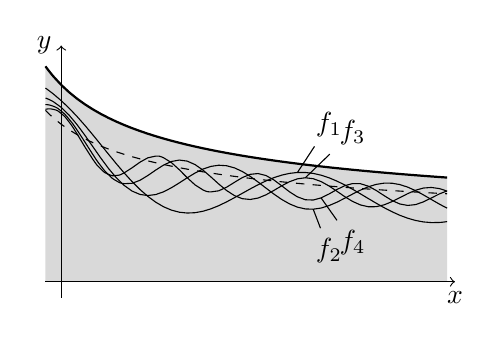
\begin{tikzpicture}
        \fill[fill = gray!30!white] (-0.2,-0.5) -- plot[smooth, tension = 1] coordinates{(-0.2,2.23607) (-0.1,2.10819) (0,2.) (0.1,1.90693) (0.2,1.82574) (0.3,1.75412) (0.4,1.69031) (0.5,1.63299) (0.6,1.58114) (0.7,1.53393) (0.8,1.49071) (0.9,1.45095) (1,1.41421) (1.1,1.38013) (1.2,1.3484) (1.3,1.31876) (1.4,1.29099) (1.5,1.26491) (1.6,1.24035) (1.7,1.21716) (1.8,1.19523) (1.9,1.17444) (2,1.1547) (2.1,1.13592) (2.2,1.11803) (2.3,1.10096) (2.4,1.08465) (2.5,1.06904) (2.6,1.05409) (2.7,1.03975) (2.8,1.02598) (2.9,1.01274) (3,1.) (3.1,0.98773) (3.2,0.9759) (3.3,0.964486) (3.4,0.953463) (3.5,0.942809) (3.6,0.932505) (3.7,0.922531) (3.8,0.912871) (3.9,0.903508) (4,0.894427) (4.1,0.885615) (4.2,0.877058) (4.3,0.868744) (4.4,0.860663) (4.5,0.852803) (4.6,0.845154) (4.7,0.837708) (4.8,0.830455) (4.9,0.823387)} -- (4.9,-0.5) -- cycle;
        \draw[->] (-0.2,-0.5) -- (5,-0.5) node[below] {$x$};
        \draw[->] (0,-0.7) -- (0,2.5) node[left] {$y$};
        \draw plot[smooth, tension = 1] coordinates{(-0.2,1.95951) (-0.1,1.88476) (0,1.8) (0.1,1.70483) (0.2,1.59993) (0.3,1.48679) (0.4,1.36748) (0.5,1.24449) (0.6,1.12056) (0.7,0.998573) (0.8,0.881369) (0.9,0.771674) (1,0.671972) (1.1,0.584416) (1.2,0.510749) (1.3,0.452247) (1.4,0.409676) (1.5,0.383271) (1.6,0.372739) (1.7,0.377272) (1.8,0.395588) (1.9,0.425981) (2,0.466392) (2.1,0.514485) (2.2,0.567738) (2.3,0.623535) (2.4,0.679263) (2.5,0.732401) (2.6,0.780614) (2.7,0.821827) (2.8,0.854301) (2.9,0.876684) (3,0.888051) (3.1,0.887932) (3.2,0.876315) (3.3,0.853637) (3.4,0.820759) (3.5,0.778921) (3.6,0.72969) (3.7,0.674891) (3.8,0.616533) (3.9,0.556729) (4,0.497615) (4.1,0.441261) (4.2,0.389601) (4.3,0.344356) (4.4,0.306974) (4.5,0.278577) (4.6,0.259925) (4.7,0.251389) (4.8,0.252951) (4.9,0.264202)};
        \draw plot[smooth, tension = 1] coordinates{(-0.2,1.83294) (-0.1,1.78684) (0,1.71429) (0.1,1.61626) (0.2,1.49659) (0.3,1.3613) (0.4,1.21788) (0.5,1.07453) (0.6,0.939467) (0.7,0.820155) (0.8,0.722763) (0.9,0.651663) (1,0.609124) (1.1,0.595188) (1.2,0.607717) (1.3,0.642633) (1.4,0.694298) (1.5,0.75602) (1.6,0.820622) (1.7,0.881045) (1.8,0.930919) (1.9,0.965066) (2,0.979888) (2.1,0.973614) (2.2,0.946392) (2.3,0.900209) (2.4,0.838673) (2.5,0.766651) (2.6,0.689818) (2.7,0.614148) (2.8,0.545391) (2.9,0.488579) (3,0.447615) (3.1,0.424958) (3.2,0.421445) (3.3,0.436252) (3.4,0.467006) (3.5,0.510019) (3.6,0.560636) (3.7,0.613662) (3.8,0.663818) (3.9,0.706207) (4,0.736724) (4.1,0.752406) (4.2,0.751658) (4.3,0.734373) (4.4,0.701911) (4.5,0.656948) (4.6,0.603226) (4.7,0.545197) (4.8,0.487628) (4.9,0.435175)};
        \draw plot[smooth, tension = 1] coordinates{(-0.2,1.75036) (-0.1,1.72908) (0,1.66667) (0.1,1.56402) (0.2,1.42916) (0.3,1.27535) (0.4,1.11865) (0.5,0.975401) (0.6,0.859772) (0.7,0.781736) (0.8,0.74578) (0.9,0.750443) (1,0.788744) (1.1,0.849394) (1.2,0.918597) (1.3,0.982151) (1.4,1.02754) (1.5,1.0457) (1.6,1.03221) (1.7,0.987807) (1.8,0.918006) (1.9,0.832142) (2,0.741799) (2.1,0.65897) (2.2,0.594218) (2.3,0.555098) (2.4,0.545094) (2.5,0.563196) (2.6,0.604173) (2.7,0.659491) (2.8,0.718699) (2.9,0.771081) (3,0.807309) (3.1,0.820835) (3.2,0.808831) (3.3,0.772534) (3.4,0.716957) (3.5,0.650026) (3.6,0.58129) (3.7,0.520407) (3.8,0.475646) (3.9,0.452631) (4,0.453525) (4.1,0.476764) (4.2,0.517365) (4.3,0.567771) (4.4,0.619067) (4.5,0.662389) (4.6,0.690299) (4.7,0.697918) (4.8,0.683633) (4.9,0.649294)};
        \draw plot[smooth, tension = 1] coordinates{(-0.2,1.68934) (-0.1,1.68969) (0,1.63636) (0.1,1.52838) (0.2,1.37934) (0.3,1.21291) (0.4,1.05656) (0.5,0.935005) (0.6,0.864597) (0.7,0.849981) (0.8,0.883523) (0.9,0.947578) (1,1.01894) (1.1,1.07437) (1.2,1.09591) (1.3,1.07478) (1.4,1.01294) (1.5,0.92223) (1.6,0.821082) (1.7,0.729963) (1.8,0.666427) (1.9,0.641057) (2,0.655176) (2.1,0.700833) (2.2,0.762971) (2.3,0.823216) (2.4,0.864348) (2.5,0.874352) (2.6,0.849136) (2.7,0.793271) (2.8,0.718661) (2.9,0.641489) (3,0.578224) (3.1,0.541664) (3.2,0.537944) (3.3,0.565224) (3.4,0.614312) (3.5,0.671037) (3.6,0.719764) (3.7,0.747191) (3.8,0.745488) (3.9,0.714077) (4,0.659609) (4.1,0.59422) (4.2,0.532486) (4.3,0.487864) (4.4,0.469457) (4.5,0.479899) (4.6,0.514833) (4.7,0.564093) (4.8,0.614255) (4.9,0.651944)};
        \draw[style = dashed] plot[smooth, tension = 1] coordinates{(-0.2,1.67705) (-0.1,1.58114) (0,1.5) (0.1,1.43019) (0.2,1.36931) (0.3,1.31559) (0.4,1.26773) (0.5,1.22474) (0.6,1.18585) (0.7,1.15045) (0.8,1.11803) (0.9,1.08821) (1,1.06066) (1.1,1.0351) (1.2,1.0113) (1.3,0.989071) (1.4,0.968246) (1.5,0.948683) (1.6,0.930261) (1.7,0.912871) (1.8,0.896421) (1.9,0.88083) (2,0.866025) (2.1,0.851943) (2.2,0.838525) (2.3,0.825723) (2.4,0.813489) (2.5,0.801784) (2.6,0.790569) (2.7,0.779813) (2.8,0.769484) (2.9,0.759555) (3,0.75) (3.1,0.740797) (3.2,0.731925) (3.3,0.723364) (3.4,0.715097) (3.5,0.707107) (3.6,0.699379) (3.7,0.691898) (3.8,0.684653) (3.9,0.677631) (4,0.67082) (4.1,0.664211) (4.2,0.657794) (4.3,0.651558) (4.4,0.645497) (4.5,0.639602) (4.6,0.633866) (4.7,0.628281) (4.8,0.622841) (4.9,0.61754)};
        \draw[style = thick] plot[smooth, tension = 1] coordinates{(-0.2,2.23607) (-0.1,2.10819) (0,2.) (0.1,1.90693) (0.2,1.82574) (0.3,1.75412) (0.4,1.69031) (0.5,1.63299) (0.6,1.58114) (0.7,1.53393) (0.8,1.49071) (0.9,1.45095) (1,1.41421) (1.1,1.38013) (1.2,1.3484) (1.3,1.31876) (1.4,1.29099) (1.5,1.26491) (1.6,1.24035) (1.7,1.21716) (1.8,1.19523) (1.9,1.17444) (2,1.1547) (2.1,1.13592) (2.2,1.11803) (2.3,1.10096) (2.4,1.08465) (2.5,1.06904) (2.6,1.05409) (2.7,1.03975) (2.8,1.02598) (2.9,1.01274) (3,1.) (3.1,0.98773) (3.2,0.9759) (3.3,0.964486) (3.4,0.953463) (3.5,0.942809) (3.6,0.932505) (3.7,0.922531) (3.8,0.912871) (3.9,0.903508) (4,0.894427) (4.1,0.885615) (4.2,0.877058) (4.3,0.868744) (4.4,0.860663) (4.5,0.852803) (4.6,0.845154) (4.7,0.837708) (4.8,0.830455) (4.9,0.823387)};
        \node (f1) at (3.4,1.5) {$f_1$};
        \node (f2) at (3.4,-0.1) {$f_2$};
        \node (f3) at (3.7,1.4) {$f_3$};
        \node (f4) at (3.7,0) {$f_4$};
        \draw (f1) -- (3,0.888051);
        \draw (f2) -- (3.2,0.421445);
        \draw (f3) -- (3.1,0.820835);
        \draw (f4) -- (3.3,0.565224);
    \end{tikzpicture}
    \caption{함수열 $\{f_i\}$가 $g$ (굵은선)에 의해 지배당하고 있다. 그림에서 $\{f_i\}$는 결국 $f$ (파선)로 점별수렴한다.}
\end{figure}

\begin{proof}
    가정으로부터 각 $f_i$에 대해 $\int_X|f_i|\,d\mu\leq\int_Xg\,d\mu<\infty$이므로 이는 적분가능하고, 비슷한 이유로 $f$도 적분가능하다. 이제 $f_i\to f$인 경우를 생각해보자. 이 경우에 함수열 $\{g-f_i\},\,\{g+f_i\}$를 생각하면 이는 음이 아닌 가측함수열로서 \texttt{Fatou}의 보조정리로부터 $\liminf_{i\to\infty}\int_Xg-f_i\,d\mu\geq\int_Xg-f\,d\mu=\int_Xg\,d\mu-\int_Xf\,d\mu$이고, $\liminf_{i\to\infty}\int_Xg-f_i\,d\mu=\int_Xg\,d\mu-\limsup_{i\to\infty}\int_Xf_i\,d\mu$에서 $\limsup_{i\to\infty}\int_Xf_i\,\mu\leq\int_Xf\,d\mu$를 얻는다. 한편, $\{g+f_i\}$에 대해서도 이와 비슷하게 하면 $\liminf_{i\to\infty}\int_Xf_i\,d\mu\geq\int_Xf\,d\mu$를 얻어 곧 $\int_Xf_i\,d\mu\to\int_Xf\,d\mu$가 된다.

    한편, $f_i\to f$ (\texttt{ae.})인 경우에 대해서는 $N=\{x\in X:f_i(x)\not\to f(x)\}$을 생각하면 이가 영집합이고 정리 \ref{thm:limitMeasurable}의 iv로부터 가측이다. 이제 함수 $h_i:X\to\overline{\mathbb{R}}$의 열 $\{h_i\}$와 함수 $h:X\to\overline{\mathbb{R}}$를 각각 $h_i=f_i\ind_{X\setminus N},\,h=f\ind_{X\setminus N}$과 같이 정의하면 $\{h_i\}$는 음이 아닌 가측함수의 열로, 증가하고 모든 $i\in\mathbb{N}$에 대해 $|h_i|\leq g$이며 $h_i\uparrow h$이다. 그렇다면 앞서 얻은 결과로부터 $\int_Xh_i\,d\mu\to\int_Xh\,d\mu$임을 바로 알 수 있고, 곧 모든 $i\in\mathbb{N}$에 대해 $f_i=h_i$ (\texttt{ae.})이며 $f=h$ (\texttt{ae.})이므로 따름정리 \ref{cor:zeroAeIntegral}의 ii로부터 $\int_Xf_i\,d\mu\to\int_Xf\,d\mu$를 얻는다.
\end{proof}

이러한 수렴정리들로부터 얻어지는 다음 결과들도 유용하다.

\begin{corollary}[Bounded convergence theorem]
    유한 측도공간 $(X,\,\mathcal{A},\,\mu)$에서 정의된 가측함수 $f_i:X\to\overline{\mathbb{R}}$의 열 $\{f_i\}$에 대해 적당한 가측함수 $f:X\to\overline{\mathbb{R}}$가 존재하여  $f_i\uparrow f$ (\texttt{ae.})라 하자. 또한, $\{f_i\}$가 균등하게 유계라 하자. 즉, 어떤 $M>0$이 존재하여 모든 $i\in\mathbb{N}$에 대해 $|f_i|\leq M$이라 하자. 그렇다면 각 $f_i$와 $f$는 적분가능하고 $\int_Xf_i\,d\mu\to\int_Xf\,d\mu$이다.
\end{corollary}

\begin{proof}
    상수 함수 $g=M$가 명백히 적분가능하므로 \texttt{DCT}로부터 이는 자명하다.
\end{proof}

\begin{corollary}
    측도공간 $(X,\,\mathcal{A},\,\mu)$에서 정의된 가측함수 $f_i:X\to\overline{\mathbb{R}}$의 열 $\{f_i\}$에 대해 다음이 성립한다.
    \begin{enumerate}
        \item 만약 각 $f_i$가 음이 아니면 $\int_X\sum_{i=1}^\infty f_i\,d\mu=\sum_{i=1}^\infty\int_Xf_i\,d\mu$이다.
        \item 만약 $\sum_{i=1}^\infty f_i$가 거의 어디서나 수렴하거나 $\pm\infty$로 발산하며,\footnotemark 적당한 적분가능한 $g:X\to\overline{\mathbb{R}}^+_0$가 존재하여 모든 $k\in\mathbb{N}$에 대해 $|\sum_{i=1}^kf_i|\leq g$라 하면 각 $f_i$와 $\sum_{i=1}^\infty f_i$는 적분가능하고 $\int_X\sum_{i=1}^\infty f_i\,d\mu=\sum_{i=1}^\infty\int_Xf_i\,d\mu$이다.
    \end{enumerate}
\end{corollary}

\begin{proof}
    각각 \texttt{MCT}와 \texttt{DCT}로부터 자명하다. 특히 ii의 경우 모든 $k\in\mathbb{N}$에 대해 $\sum_{i=1}^kf_i$가 적분가능하므로 곧 임의의 $i\in\mathbb{N}$에 대해 $f_i=\sum_{j=1}^if_j-\sum_{j=1}^{i-1}f_j$가 적분가능함을 안다.
\end{proof}

\begin{corollary}\label{cor:integralContinuous}
    측도공간 $(X,\,\mathcal{A},\,\mu)$와 열린집합 $U\subseteq\mathbb{R}^n$ 대해 함수 $f:X\times U\to\mathbb{R}$가 다음을 조건을 만족한다고 하자.
    \begin{enumerate}
        \item 임의의 $y\in U$에 대해 함수 $x\mapsto f(x,\,y)$가 적분가능하다.
        \item 거의 대부분의 $x\in X$에 대해 함수 $y\mapsto f(x,\,y)$가 연속이다.
        \item 적당한 적분가능한 함수 $g:X\to\overline{\mathbb{R}}^+_0$가 존재하여 $X\times U$에서 $|f|\leq g$이다.
    \end{enumerate}
    그렇다면 함수 $y\mapsto\int_Xf(x,\,y)\,d\mu(x)$는 연속이다.
\end{corollary}

\begin{proof}
    \texttt{DCT}로부터 거의 자명하다. 임의의 $y\in U$를 고정하고 $U$에 속하는 임의의 수열 $\{y_i\}$를 생각하여 $y_i\to y$라 하면 주어진 조건으로부터 거의 대부분의 $x\in X$에 대해 $f(x,\,y_i)\to f(x,\,y)$이고 임의의 $i\in\mathbb{N}$와 임의의 $x\in X$에 대해 $|f(x,\,y_i)|\leq g(x)$이므로, 곧 \texttt{DCT}에서 $\lim_{i\to\infty}\int_Xf(x,\,y_i)\,d\mu(x)=\int_Xf(x,\,y)\,d\mu(x)$가 되어 증명이 끝난다.
\end{proof}

\begin{corollary}[Leibniz's rule]\label{cor:leibnizRule}
    측도공간 $(X,\,\mathcal{A},\,\mu)$와 열린집합 $U\subseteq\mathbb{R}$ 대해 함수 $f:X\times U\to\mathbb{R}$가 다음 조건을 만족한다고 하자.
    \begin{enumerate}
        \item 임의의 $y\in U$에 대해 함수 $x\mapsto f(x,\,y)$가 적분가능하다.
        \item 거의 대부분의 $x\in X$에 대해 함수 $y\mapsto f(x,\,y)$가 미분가능하다.
        \item 임의의 $y\in U$에 대해 함수 $x\mapsto(\partial/\partial y)f(x,\,y)$가 가측이다.\footnotemark
        \item 적당한 적분가능한 함수 $g:X\to\overline{\mathbb{R}}^+_0$가 존재하여 $X\times U$에서 $|\partial f/\partial y|\leq g$이다.
    \end{enumerate}
    그렇다면 함수 $y\mapsto\int_Xf(x,\,y)\,d\mu(x)$는 미분가능하고 임의의 $y\in U$에 대해 함수 $x\mapsto(\partial f/\partial y)(x,\,y)$는 적분가능하며 다음이 성립한다.
    \begin{equation*}
        \frac{d}{dy}\int_Xf(x,\,y)\,d\mu(x)=\int_X\frac{\partial}{\partial y}f(x,\,y)\,d\mu(x)
    \end{equation*}
\end{corollary}

\begin{proof}
    편의를 위해 함수 $f_x:U\to\mathbb{R}$를 $f_x:y\mapsto f(x,\,y)$로 정의하자. 이제 임의의 $y\in U$를 고정하고 적당한 열린 \texttt{ball} $B$에 대해 함수 $k:X\times B\to\mathbb{R}$를
    \begin{align*}
        (x,\,h)\mapsto\begin{dcases*}
            \dfrac{f(x,\,y+h)-f(x,\,y)}{h}&$h\ne0$ 이고 $f_x$가 미분가능한 경우\\
            \dfrac{\partial}{\partial y}f(x,\,y)&$h=0$ 이고 $f_x$가 미분가능한 경우\\
            0&\texttt{ow.}
        \end{dcases*}
    \end{align*}
    로 정의하면 이는 \texttt{well-define}되고, 만약 이가 따름정리 \ref{cor:integralContinuous}의 조건을 모두 만족함을 보일 수 있으면 곧바로
    \begin{align*}
        \lim_{h\to 0}\int_X\frac{f(x,\,y+h)-f(x,\,y)}{h}\,d\mu(x)&=\lim_{h\to 0}\int_Xk(x,\,h)\,d\mu(x)\\
        &=\int_X\frac{\partial}{\partial y}f(x,\,y)\,d\mu(x)
    \end{align*}
    가 되어 증명이 끝난다. 그런데 주어진 조건으로부터 따름정리 \ref{cor:integralContinuous}의 조건 i, ii가 만족됨은 자명하므로 iii이 만족됨을 보이는 것만 보이자. 임의의 $(x,\,h)\in X\times V$에 대해 만약 $f_x$가 미분가능하지 않다면 $k(x,\,h)=0$에서 $|k(x,\,h)|\leq g(x)$임이 분명하므로 $f_x$가 미분가능하다고 하자. 그렇다면 $h=0$인 경우에는 가정으로부터 $|k(x,\,h)|=|(\partial f/\partial y)(x,\,y)|\leq g(x)$이고, 그렇지 않은 경우에는 \texttt{MVT}에서 $y$와 $y+h$ 사이의 적당한 $z\in U$가 존재하여 $|k(x,\,h)|=|(\partial f/\partial y)(x,\,z)|\leq g(x)$가 되어 iii이 만족된다. 증명은 이로써 충분하다.
\end{proof}

측도를 이용해 적분을 정의한 것과 반대로 적분을 이용해 새로운 측도를 유도할 수도 있다. 이러한 기법은 확률론에서 널리 쓰이므로 여기서 잠시 살펴보는 것이 좋을 것 같다.

\begin{theorem}
    측도공간 $(X,\,\mathcal{A},\,\mu)$에서 정의된 음이 아닌 가측함수 $f:X\to\overline{\mathbb{R}}^+_0$에 대해 함수 $\mu_f:\mathcal{A}\to\overline{\mathbb{R}}^+_0$를 $\mu_f:A\mapsto\int_Af\,d\mu$로 두면 $\mu_f$는 $\mathcal{A}$ 위의 측도이다.
\end{theorem}

\begin{proof}
    당장 $\mu_f(\emptyset)=0$임은 분명하므로 $\mu_f$가 $\sigma$-가법성을 가짐을 보이는 것으로 충분하다. 이를 위해 $\mathcal{A}$에 속하는 임의의 집합열 $\{A_i\}$를 택하면 \texttt{MCT}에서 $\mu_f(\bigsqcup_{i=1}^\infty A_i)=\int_{\bigsqcup_{i=1}^\infty A_i}f\,d\mu=\int_X\sum_{i=1}^\infty f\ind_{A_i}\,d\mu=\sum_{i=1}^\infty\int_{A_i}f\,d\mu=\sum_{i=1}^\infty\mu_f(A_i)$가 되어 $\mu_f$가 $\sigma$-가법성을 가짐을 알고, 곧 증명이 끝난다.
\end{proof}

\begin{definition}
    가측공간 $(X,\,\mathcal{A},\,\mu)$에서 정의된 음이 아닌 가측함수 $f:X\to\overline{\mathbb{R}}^+_0$에 대해 \textbf{$f$로부터 유도되는 측도(\texttt{measure induced by} $f$)}를 $\mu_f$로 쓰고 $\mathcal{A}$ 위의 측도 $\mu_f:A\mapsto\int_Af\,d\mu$로 정의한다.
\end{definition}

그렇다면 과연 이의 역도 성립할까에 대한 궁금증이 자연스럽게 피어난다. 어떤 고정된 측도 $\mu$에 대해 임의의 측도 $\nu$를 적당한 음이 아닌 가측함수 $f$를 사용하여 $\mu_f=\nu$와 같이 쓸 수 있을까? 만약 그렇다면 이러한 $f$는 유일할까? 만약 그 존재성이 일반적으로 보장되는 것이 아니라면, 어떤 조건에서 존재성을 말할 수 있을까? 이런 질문들에 대한 답은 자연스럽게 도함수의 일반화에 대한 아이디어로 이어지고, 이는 확률론이 꽃필 수 있는 견고한 기반이 된다. 다만, 그 자체로 꽤나 많은 논의가 필요하므로 일단 이와 관련된 논의는 잠시 미뤄두고, 여기에서는 적분에 관한 이야기를 마저 하도록 하자.

\begin{theorem}\label{thm:monoSeriesIntegral}
    측도공간 $(X,\,\mathcal{A},\,\mu)$에서 정의된 음이 아닌 가측함수 $f:X\to\overline{\mathbb{R}}^+_0$와 $\mathcal{A}$에 속하는 집합열 $\{A_i\}$에 대해 다음이 성립한다.
    \begin{enumerate}
        \item 만약 $A_i\uparrow A$이면 $\int_{A_i}f\,d\mu\uparrow\int_Af\,d\mu$이다.
        \item 만약 $A_i\downarrow A$이고 $f$가 $A_1$ 위에서 적분가능하면 $\int_{A_i}f\,d\mu\downarrow\int_Af\,d\mu$이다.
    \end{enumerate}
    한편, 적분가능한 함수 $f:X\to\overline{\mathbb{R}}$에 대해서도 위의 성질들이 성립한다. 특히 ii의 경우 $f$의 $A_1$ 위에서의 적분가능성이 자명해지므로 이 조건을 생략할 수 있다.
    \begin{enumerate}
        \item[ii$^\circ$] 만약 $A_i\downarrow A$이면 $\int_{A_i}f\,d\mu\downarrow\int_Af\,d\mu$이다.
    \end{enumerate}
\end{theorem}

\begin{proof}
    이는 $\mu_f$가 $\mathcal{A}$ 위에서의 측도를 이루므로 자명하다. 한편, 적분가능한 함수 $f:X\to\overline{\mathbb{R}}$에 대해서는 이를 각각 양과 음의 부분으로 나누어 각각이 $\mathcal{A}$ 위에서의 측도를 유도한다는 사실을 이용하면 된다.
\end{proof}

\begin{theorem}\label{thm:intInducedMeasure}
    측도공간 $(X,\,\mathcal{A},\,\mu)$에서 정의된 음이 아닌 가측함수 $f,\,g:X\to\overline{\mathbb{R}}^+_0$에 대해 $\int_Xg\,d\mu_f=\int_Xfg\,d\mu$이다. 한편, $\mu_f$-적분가능한(혹은 $fg$가 $\mu$-적분가능한 가측함수) $g:X\to\overline{\mathbb{R}}$에 대해서도 동일한 결과가 성립하며 이때 $fg$는 $\mu$-적분가능하다(혹은 $g$는 $\mu_f$-적분가능하다).
\end{theorem}

\begin{proof}
    먼저 $g$가 음이 아닌 단순함수인 경우를 생각하여 이의 표준형을 $g=\sum_{i=1}^ka_i\ind_{A_i}$라 하자. 그렇다면 $\int_Xg\,d\mu_f=\sum_{i=1}^ka_i\mu_f(A_i)=\sum_{i=1}^ka_i\int_{A_i}f\,d\mu=\int_X\sum_{i=1}^na_if\ind_{A_i}\,d\mu=\int_Xfg\,d\mu$임이 분명하다. 이제 $g$를 음이 아닌 가측함수라 하면 정리 \ref{thm:measurableFunctionApprox}로부터 음이 아닌 단순함수 $g_i:X\to\mathbb{R}^+_0$의 열 $\{g_i\}$가 존재하여 $g_i\uparrow g$이므로 \texttt{MCT}에서 $\int_Xgd\mu_f=\lim_{i\to\infty}\int_Xg_id\mu_f=\lim_{i\to\infty}\int_Xfg_id\mu=\int_Xfgd\mu$이다.

    한편, $\mu_f$-적분가능한 $g:X\to\overline{\mathbb{R}}$에 대해서, 이를 양과 음의 부분으로 나누어 앞선 결과를 적용하면 $fg$가 $\mu$-적분가능하며 $\int_Xg\,d\mu_f=\int_Xfg\,d\mu$임을 쉽게 알 수 있고, $fg$가 $\mu$-적분가능한 가측함수 $g:X\to\overline{\mathbb{R}}$에 대해서도 비슷하게 하면 된다.
\end{proof}

\begin{theorem}\label{thm:twoFuncIntEqual}
    측도공간 $(X,\,\mathcal{A},\,\mu)$에서 정의된 음이 아닌 가측함수 $f,\,g:X\to\overline{\mathbb{R}}^+_0$에 대해 만약 $\mu$가 $\sigma$-유한하며 임의의 $A\in\mathcal{A}$에 대해 $\int_Af\,d\mu=\int_Ag\,d\mu$이면 $f=g$ (\texttt{ae.})이다. 한편, 적분가능한 $f,\,g:X\to\overline{\mathbb{R}}$에 대해서도 동일한 결과가 성립하며, 이 경우에는 $\mu$가 $\sigma$-유한하다는 조건을 생략할 수 있다.
\end{theorem}

\begin{proof}
    가정으로부터 $\mathcal{A}$에 속하는 적당한 집합열 $\{A_i\}$가 존재하여 $\mu(A_i)<\infty$이고 $\bigcup_{i=1}^\infty A_i=X$이고, \texttt{WLOG}, 필요하다면 각 항을 $C_i:=\bigcup_{j=1}^iA_j$로 바꾸어 $\{A_i\}$가 처음부터 증가하는 집합열이라 해도 된다. 이제 집합열 $\{B_i\}$를 $B_i:=\{x\in X:f(x)<g(x),\,f(x)<i\}$로 두면 이는 $\mathcal{A}$에 속하는 집합열이며 모든 $i\in\mathbb{N}$에 대해 $\int_{A_i\cap B_i}f\,d\mu=\int_{A_i\cap B_i}g\,d\mu\leq\int_{A_i\cap B_i}i\,d\mu=i\mu(A_i\cap B_i)<\infty$이다. 이로부터 각 $i\in\mathbb{N}$에 대해 $\int_{A_i\cap B_i}g-f\,d\mu=0$이고, 이는 보조정리 \ref{cor:zeroAeIntegral}의 iii으로부터 $A_i\cap B_i$가 영집합임을 의미하므로 $\{x\in X:f(x)<g(x)\}=\bigcup_{i=1}^\infty(A_i\cup B_i)$도 영집합이 되어 $f\geq g$ (\texttt{ae.})이다. 한편, 비슷하게 하면 $f\leq g$ (\texttt{ae.})임도 보일 수 있으므로 곧 $f=g$ (\texttt{ae.})임을 안다.

    한편, 적분가능한 $f,\,g:X\to\overline{\mathbb{R}}$에 대해서도 비슷하게 하면 된다. 다만, 이 경우에는 $f,\,g$가 적분가능하여 $\int_{B_i}f\,d\mu=\int_{B_i}g\,d\mu<\infty$이므로 $\mu$가 $\sigma$-유한하다는 조건이 필요하지 않다.
\end{proof}

측도공간의 완비화와 관련된 정리를 끝으로 길었던 \texttt{Lebesgue} 적분론의 전개를 마무리하도록 하겠다.

\begin{theorem}\label{thm:measureCompletionInt}
    측도공간 $(X,\,\mathcal{A},\,\mu)$에서 정의된 음이 아닌 $\mathcal{A}/\mathcal{B}_1$-가측함수 $f:X\to\overline{\mathbb{R}}^+_0$에 대해 $\int_Xf\,d\mu=\int_Xf\,d\overline{\mu}$이다. 한편, $\mu$-적분가능한(혹은 $\overline{\mu}$-적분가능한 $\mathcal{A}/\mathcal{B}_1$-가측함수) $f:X\to\overline{\mathbb{R}}$에 대해서도 동일한 결과가 성립하며 이때 $f$는 $\overline{\mu}$-적분가능하다(혹은 $\mu$-적분가능하다).
\end{theorem}

\begin{proof}
    먼저 $f$가 음이 아닌 단순함수인 경우를 생각하여 이의 표준형을 $f=\sum_{i=1}^ka_i\ind_{A_i}$라 하자. 그렇다면 $\int_Xf\,d\mu=\sum_{i=1}^ka_i\mu(A_i)=\sum_{i=1}^ka_i\overline{\mu}(A_i)=\int_Xf\,d\overline{\mu}$임이 분명하다. 이제 $f$를 음이 아닌 가측함수라 하면 정리 \ref{thm:measurableFunctionApprox}로부터 음이 아닌 단순함수 $f_i:X\to\mathbb{R}^+_0$의 열 $\{f_i\}$가 존재하여 $f_i\uparrow f$이므로 \texttt{MCT}에서 $\int_Xf\,d\mu=\lim_{i\to\infty}\int_Xf_i\,d\mu=\lim_{i\to\infty}\int_Xf_i\,d\overline{\mu}=\int_Xf\,d\overline{\mu}$이다.

    한편, $\mu$-적분가능한 $f:X\to\overline{\mathbb{R}}$에 대해서, 이를 양과 음의 부분으로 나누어 앞선 결과를 적용하면 $f$가 $\overline{\mu}$-적분가능하며 $\int_Xf\,d\mu=\int_Xf\,d\overline{\mu}$임을 쉽게 알 수 있고, $\overline{\mu}$-적분가능한 $\mathcal{A}/\mathcal{B}_1$-가측함수 $f:X\to\overline{\mathbb{R}}$에 대해서도 비슷하게 하면 된다.
\end{proof}

\section{Product Measures and Contruction of The Lebesgue Measure II}

이전 절에서 \texttt{Lebesgue} 적분론의 전개가 마무리 되었으므로 이제 우리의 원래 목적으로 되돌아와 \texttt{Lebesgue} 측도의 두 번째 구성을 본격적으로 시작해보려고 한다. 앞서 언급했듯이 이를 위해서는 우선 적당한 곱연산을 정의해야 한다.

\begin{definition}
    가측공간 $(X,\,\mathcal{A}),\,(Y,\,\mathcal{B})$에 대해 적당한 $A\in\mathcal{A},\,B\in\mathcal{B}$가 존재하여 $C=A\times B$로 쓸 수 있는 집합 $C\subseteq X\times Y$를 \textbf{\texttt{measurable rectangle}}이라 하고, 모든 measurable rectangle의 모임을 $\mathcal{A}\times\mathcal{B}$로 쓴다. 이때 $\sigma(\mathcal{A}\times\mathcal{B})$를 $\mathcal{A},\,\mathcal{B}$의 \textbf{\texttt{product} $\sigma$-\texttt{algebra}}라 하며 $\mathcal{A}\otimes\mathcal{B}$로 쓴다.
\end{definition}

위의 정의로부터 $\sigma$-대수의 $\times$곱은 결합법칙을 만족함이 분명하다. 따라서 가측공간 $(X_1,\,\mathcal{A}_1),\,\cdots,\,(X_i,\,\mathcal{A}_k)$에 대해 $\prod_{i=1}^k\mathcal{A}_i:=\mathcal{A}_1\times\cdots\times\mathcal{A}_k$가 \texttt{well-define}된다. 한편, $\sigma$-대수의 $\otimes$곱이 결합법칙을 만족하는가는 조금 덜 자명하다.

\begin{theorem}\label{thm:productSigmaAlgebraAssoci}
    가측공간 $(X,\,\mathcal{A}),\,(Y,\,\mathcal{B}),\,(Z,\,\mathcal{C})$에 대해 $(\mathcal{A}\otimes\mathcal{B})\otimes\mathcal{C}=\mathcal{A}\otimes(\mathcal{B}\otimes\mathcal{C})=\sigma(\mathcal{A}\times\mathcal{B}\times\mathcal{C})$이다.
\end{theorem}

\begin{proof}
    표기의 편의를 위해 $\mathcal{D}=\sigma(\mathcal{A}\times\mathcal{B}\times\mathcal{C})$라 하자. 만약 $(\mathcal{A}\otimes\mathcal{B})\otimes\mathcal{C}=\mathcal{A}\otimes(\mathcal{B}\otimes\mathcal{C})=\mathcal{D}$임을 보일 수 있으면 증명이 끝난다. 이를 위해 임의의 $C\in\mathcal{C}$를 고정하고 $\mathcal{E}=\{A\in\mathcal{A}\otimes\mathcal{B}:A\times C\in\mathcal{D}\}$를 생각하면 $X\times Y\in\mathcal{E}$임이 분명하다. 또한, 임의의 $A\in\mathcal{E}$에 대해 $A^c\times C=[(X\times Y)\times C]\setminus (A\times C)\in\mathcal{D}$에서 $\mathcal{E}$는 여집합에 대해 닫혀있다. 한편, $\mathcal{E}$에 속하는 임의의 서로소인 집합열 $\{A_i\}$에 대해 $(\bigsqcup_{i=1}^\infty A_i)\times C=\bigsqcup_{i=1}^\infty(A_i\times C)\in\mathcal{D}$이므로 이상으로부터 $\mathcal{E}$이 $\lambda$-\texttt{system}임을 알 수 있다. 한편, 임의의 $A,\,B\in\mathcal{E}$에 대해 $(A\cap B)\times C=(A\times C)\cap(B\times C)\in\mathcal{E}$에서 $\mathcal{E}$는 교집합에 대해서도 닫혀있어 곧 $\pi$-\texttt{system}이기도 하다. 그렇다면 보조정리 \ref{lem:Dynkin}로부터 $\mathcal{E}$는 $\sigma$-대수이고, 정의로부터 $\mathcal{A}\times\mathcal{B}\subseteq\mathcal{E}$임이 분명하므로 $\mathcal{A}\otimes\mathcal{B}\subseteq\mathcal{E}$이다. 이제 이상의 결과가 임의의 $C\in\mathcal{C}$에 대해 성립함을 상기한다면 $(\mathcal{A}\otimes\mathcal{B})\times\mathcal{C}\subseteq\mathcal{D}$가 되어 곧 $(\mathcal{A}\otimes\mathcal{B})\otimes\mathcal{C}\subseteq\mathcal{D}$이다. 한편, $\mathcal{A}\times\mathcal{B}\times\mathcal{C}\subseteq(\mathcal{A}\otimes\mathcal{B})\otimes\mathcal{C}$가 분명하므로 $\mathcal{D}\subseteq(\mathcal{A}\otimes\mathcal{B})\otimes\mathcal{C}$에서 역의 포함관계도 성립하고, 곧 $(\mathcal{A}\otimes\mathcal{B})\otimes\mathcal{C}=\mathcal{D}$이다. 비슷한 방법으로 $\mathcal{A}\otimes(\mathcal{B}\otimes\mathcal{C})=\mathcal{D}$도 보일 수 있다.
\end{proof}

이로부터 $\sigma$-대수의 $\otimes$곱도 결합법칙을 만족하므로 $\bigotimes_{i=1}^k\mathcal{A}_i=\mathcal{A}_1\otimes\cdots\otimes\mathcal{A}_k$가 \texttt{well-define}된다. 만약 $\mathcal{A}_1=\cdots=\mathcal{A}_k=:\mathcal{A}$이면 이들의 $\otimes$곱을 $\mathcal{A}^{\otimes k}$로 간단히 쓰기도 한다.

\begin{definition}
    집합 $X,\,Y$와 $A\subseteq X\times Y$, 점 $x_0\in X,\,y_0\in Y$에 대해 $A$의 \textbf{\texttt{section}} $A_{x_0},\,A^{y_0}$를 각각 $A_{x_0}=\{y\in Y:(x_0,\,y)\in A\},\,A^{y_0}=\{x\in X:(x,\,y_0)\in A\}$로 정의한다.
\end{definition}

\begin{definition}
    집합 $X,\,Y,\,Z$와 함수 $f:X\times Y\to Z$, 점 $x_0\in X,\,y_0\in Y$에 대해 $f$의 \textbf{\texttt{section}} $f_{x_0}:Y\to Z,\,f^{y_0}:X\to Z$를 각각 $f_{x_0}:y\mapsto f(x_0,\,y),\,f^{y_0}:x\mapsto f(x,\,y_0)$로 정의한다.
\end{definition}

\begin{figure}[!ht]
    \centering
    \subfigure{
    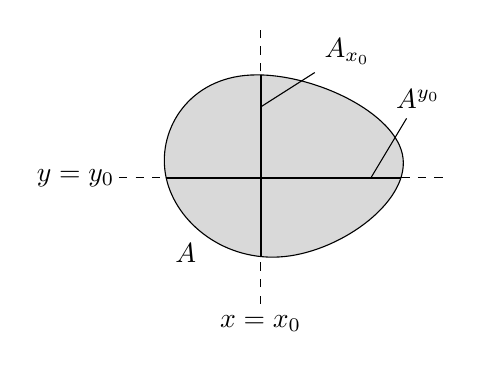
\begin{tikzpicture}
        \begin{scope}[style = dashed]
            \draw (0.9,1) -- (5.1,1);
            \draw (2.7,-0.6) -- (2.7,2.9);
        \end{scope}
        \draw[fill = gray!30!white] plot[smooth cycle, tension = 0.9] coordinates{(1.5,1) (3,0) (4.5,1.3) (2.5,2.3)};
        \begin{scope}[style = thick]
            \clip plot[smooth cycle, tension = 0.9] coordinates{(1.5,1) (3,0) (4.5,1.3) (2.5,2.3)};
            \draw (0.9,1) -- (5.1,1);
            \draw (2.7,-0.6) -- (2.7,2.9);
        \end{scope}
        \node at (0.35,1) {$y=y_0$};
        \node at (2.7,-0.85) {$x=x_0$};
        \node at (1.75,0.05) {$A$};
        \node (a) at (3.8,2.6) {$A_{x_0}$};
        \node (b) at (4.7,2) {$A^{y_0}$};
        \draw (2.7,1.9) -- (a);
        \draw (4.1,1) -- (b);
    \end{tikzpicture}
    }
    \qquad
    \subfigure{
    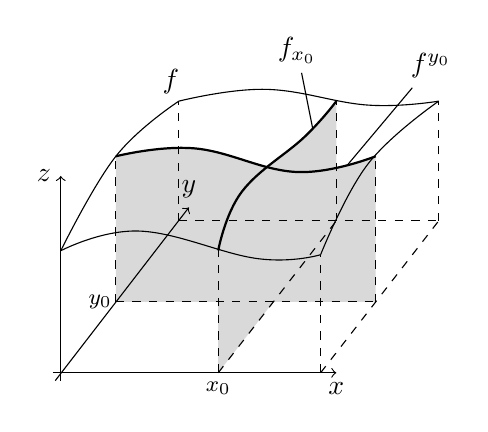
\begin{tikzpicture}
        \begin{scope}[fill = gray!30!white]
            \fill plot[smooth, tension = 0.7] coordinates{(2,1.555) (2.3,2.3) (3.1,3) (3.5,3.45)} -- (3.5,1.93) -- (2,0) -- cycle;
            \fill plot[smooth, tension = 0.7] coordinates{(0.7,2.75) (1.7,2.85) (3,2.55) (4,2.75)} -- (4,0.9) -- (0.7,0.9) -- cycle;
        \end{scope}
        \draw[->] (0,-0.1) -- (0,2.5) node[left] {$z$};
        \draw[->] (-0.1,0) -- (3.5,0) node[below] {$x$};
        \draw[->] (-0.07,-0.1) -- (1.627,2.1) node[above] {$y$};
        \draw plot[smooth, tension = 0.7] coordinates{(0,1.55) (1,1.8) (2.5,1.45) (3.3,1.5)};
        \draw plot[smooth, tension = 0.7] coordinates{(1.5,3.45) (2.6,3.6) (3.9,3.4) (4.8,3.45)};
        \draw plot[smooth, tension = 0.7] coordinates{(0,1.55) (0.7,2.75) (1.5,3.45)};
        \draw plot[smooth, tension = 0.7] coordinates{(3.3,1.5) (3.9,2.65) (4.8,3.45)};
        \begin{scope}[style = thick]
            \draw plot[smooth, tension = 0.7] coordinates{(2,1.555) (2.3,2.3) (3.1,3) (3.5,3.45)};
            \draw plot[smooth, tension = 0.7] coordinates{(0.7,2.75) (1.7,2.85) (3,2.55) (4,2.75)};
        \end{scope}
        \begin{scope}[style = dashed]
            \draw (2,0) -- (2,1.555);
            \draw (3.3,0) -- (3.3,1.5);
            \draw (1.5,1.93) -- (1.5,3.45);
            \draw (4.8,1.93) -- (4.8,3.45);
            \draw (3.5,1.93) -- (3.5,3.45);
            \draw (1.5,1.93) -- (4.8,1.93);
            \draw (3.3,0) -- (4.8,1.93);
            \draw (2,0) -- (3.5,1.93);
            \draw (0.7,0.9) -- (0.7,2.75);
            \draw (4,0.9) -- (4,2.75);
            \draw (0.7,0.9) -- (4,0.9);
        \end{scope}
        \node at (1.4,3.7) {$f$};
        \node (a) at (4.7,3.9) {$f^{y_0}$};
        \node (b) at (3,4.1) {$f_{x_0}$};
        \draw (3.65,2.65) -- (a);
        \draw (3.2,3.1) -- (b);
        \begin{scope}[every node/.append style = {font = \footnotesize}]
            \node at (2,-0.2) {$x_0$};
            \node at (0.5,0.9) {$y_0$};
        \end{scope}
    \end{tikzpicture}
    }
    \caption{집합 $A\subseteq\mathbb{R}^2$(왼쪽)와 함수 $f:\mathbb{R}^2\to\mathbb{R}$(오른쪽)의 \texttt{section}들.}
\end{figure}

다음 정리에 따르면 \texttt{product} $\sigma$-\texttt{algebra}에 속하는 \texttt{measurable rectangle}을 포함한 모든 집합은 항상 가측인 \texttt{section}을 가진다. 이로써 우리는 \texttt{product} $\sigma$-\texttt{algebra}의 구조를 조금 더 잘 이해할 수 있다.

\begin{theorem}\label{thm:sectionMeasurable}
    가측공간 $(X,\,\mathcal{A}),\,(Y,\,\mathcal{B}),\,(Z,\,\mathcal{C})$에 대해 다음이 성립한다.
    \begin{enumerate}
        \item 임의의 $A\in\mathcal{A}\otimes\mathcal{B}$와 임의의 $x\in X,\,y\in Y$에 대해 $A_x\in\mathcal{B},\,A^y\in\mathcal{A}$이다.
        \item $\mathcal{A}\otimes\mathcal{B}/\mathcal{C}$-가측함수 $f:X\times Y\to Z$와 임의의 $x\in X,\,y\in Y$에 대해 $f_x,\,f^y$는 각각 $\mathcal{B}/\mathcal{C}$-가측이고 $\mathcal{A}/\mathcal{C}$-가측이다.
    \end{enumerate}
\end{theorem}

\begin{proof}
    i. 임의의 $x\in X$를 고정하고 $\mathcal{D}=\{A\in\mathcal{A}\otimes\mathcal{B}:A_x\in\mathcal{B}\}$를 생각하면 임의의 $A\times B\in\mathcal{A}\times\mathcal{B}$에 대해
    \begin{equation*}
        (A\times B)_x=
        \begin{dcases*}
            B&$x\in A$인 경우\\
            \emptyset&\texttt{ow.}
        \end{dcases*}
    \end{equation*}
    이므로 $\mathcal{A}\times\mathcal{B}\subseteq\mathcal{D}$이고, 따라서 $\mathcal{D}$가 $\sigma$-대수라는 것만 보이면 $\mathcal{A}\otimes\mathcal{B}\subseteq\mathcal{D}$가 되어 증명이 끝난다. 이를 위해 임의의 $A\in\mathcal{D}$를 생각하면 $(A^c)_x=(A_x)^c\in\mathcal{B}$이므로 $A^c\in\mathcal{D}$에서 $\mathcal{D}$는 여집합에 대해 닫혀있다. 또한 $\mathcal{D}$에 속하는 임의의 집합열 $\{A_i\}$에 대해 $(\bigcup_{i=1}^\infty A_i)_x=\bigcup_{i=1}^\infty(A_i)_x\in\mathcal{B}$이므로 $\bigcup_{i=1}^\infty A_i\in\mathcal{D}$에서 $\mathcal{D}$는 가산 합집합에 대해서도 닫혀있다. 이제 이가 공집합이 아님은 분명하므로 곧 $\sigma$-대수이고, 증명이 끝난다. 한편, $A^y$에 대해서도 이와 비슷하게 하면 된다.

    ii. 임의의 $A\in\mathcal{C}$에 대해 $(f_x)^{-1}(A)=[f^{-1}(A)]_x$이고 $(f^y)^{-1}(A)=[f^{-1}(A)]^y$이므로 이는 i로부터 자명하다.
\end{proof}

이제 \texttt{product} $\sigma$-\texttt{algebra}에 측도를 부여하는 방법에 대해 생각해보자. 만약 곱해지는 두 가측공간에 적당한 측도가 정의되어 있었다면 이를 사용하면서도 곱셈이라는 구조를 잘 반영할 수 있도록 \texttt{product} $\sigma$-\texttt{algebra}에 측도를 부여하는 것이 자연스러울 것이다. 이런 관점에서, 다음 정리는 \texttt{product} $\sigma$-\texttt{algebra}에 자연스러운 측도를 정의할 구체적인 방법을 제공하는 동시에, 이러한 측도의 유일성까지 보장한다.

\begin{lemma}\label{lem:productMeasure}
    $\sigma$-유한 측도공간 $(X,\,\mathcal{A},\,\mu),\,(Y,\,\mathcal{B},\,\nu)$와 임의의 $A\in\mathcal{A}\otimes\mathcal{B}$에 대해 함수 $\varphi_A:X\to\overline{\mathbb{R}}^+_0$를 $\varphi_A:x\mapsto\nu(A_x)$로 정의하면 이는 $\mathcal{A}/\mathcal{B}_1$-가측이다. 비슷하게, 함수 $\psi_A:Y\to\overline{\mathbb{R}}^+_0$를 $\psi_A:y\mapsto\mu(A^y)$로 정의하면 이는 $\mathcal{B}/\mathcal{B}_1$-가측이다.
\end{lemma}

\begin{proof}
    먼저 $\nu$가 유한한 경우를 생각하여 $\mathcal{L}=\{A\in\mathcal{A}\otimes\mathcal{B}:\varphi_A\textrm{가 $\mathcal{A}/\mathcal{B}_1$-가측}\}$을 생각하면 임의의 $A\times B\in\mathcal{A}\times\mathcal{B}$에 대해 $\varphi_{A\times B}(x)=\nu((A\times B)_x)=\nu(B)\ind_A(x)$이므로 이가 단순함수가 되어 $A\times B\in\mathcal{L}$이고, 곧 $\mathcal{A}\times\mathcal{B}\subseteq\mathcal{L}$이다. 이제 $\mathcal{A}\times\mathcal{B}$가 $\pi$-\texttt{system}임은 분명하므로 만약 우리가 $\mathcal{L}$이 $\lambda$-\texttt{system}임을 보일 수 있으면 \texttt{Dynkin}의 $\pi$-$\lambda$ 정리로부터 $\mathcal{L}=\mathcal{A}\otimes\mathcal{B}$가 되어 증명이 끝난다. 이를 위해 임의의 $A\in\mathcal{L}$를 택하면 $\varphi_{A^c}(x)=\nu((A^c)_x)=\nu(Y\setminus A_x)=\nu(Y)-\nu(A_x)=\nu(Y)-\varphi_A(x)$에서 이가 $\mathcal{A}/\mathcal{B}_1$-가측이므로 $A^c\in\mathcal{L}$이고, 곧 $\mathcal{L}$은 여집합에 대해 닫혀있다. 또한, $\mathcal{L}$에 속하는 임의의 서로소인 집합열 $\{A_i\}$에 대해 $\varphi_{\bigsqcup_{i=1}^\infty A_i}(x)=\nu((\bigsqcup_{i=1}^\infty A_i)_x)=\nu(\bigsqcup_{i=1}^\infty(A_i)_x)=\sum_{i=1}^\infty\nu((A_i)_x)=\sum_{i=1}^\infty\varphi_{A_i}(x)$에서 이가 $\mathcal{A}/\mathcal{B}_1$-가측이므로 $\bigsqcup_{i=1}^\infty A_i\in\mathcal{L}$이고, $X\times Y\in\mathcal{L}$임은 분명하므로 곧 $\mathcal{L}$이 $\lambda$-\texttt{system}이 되어 증명이 끝난다.

    한편, $\nu$가 $\sigma$-유한한 경우에는 정의로부터 $\mathcal{B}$에 속하는 적당한 집합열 $\{B_i\}$가 존재하여 각 $i\in\mathbb{N}$에 대해 $\nu(B_i)<\infty$이고 $\bigcup_{i=1}^\infty B_i=Y$이다. \texttt{WLOG}, 필요하다면 각 항을 $C_i:=B_i\setminus\bigcup_{j=1}^{i-1}A_j$로 바꾸어 $\{B_i\}$가 처음부터 서로소였다고 해도 된다. 이제 각 $i\in\mathbb{N}$에 대해 측도 $\nu_{B_i}$가 유한하므로 곧 임의의 $A\in\mathcal{A}\otimes\mathcal{B}$에 대해 함수 $\varphi_A^i:X\to\overline{\mathbb{R}}^+_0$를 $\varphi_A^i:x\mapsto\nu_{B_i}(A_x)$로 두면 앞선 결과로부터 이가 $\mathcal{A}/\mathcal{B}_1$-가측이고, 곧 $\varphi_A=\sum_{i=1}^\infty \varphi_A^i$에서 $\varphi_A$가 $\mathcal{A}/\mathcal{B}_1$-가측이다. 남은 $\psi_A$에 대해서도 비슷하게 하면 된다.
\end{proof}

\begin{theorem}\label{thm:productMeasure}
    $\sigma$-유한 측도공간 $(X,\,\mathcal{A},\,\mu),\,(Y,\,\mathcal{B},\,\nu)$에 대해 적당한 $\mathcal{A}\otimes\mathcal{B}$ 위의 측도 $\mu\otimes\nu:\mathcal{A}\otimes\mathcal{B}\to\overline{\mathbb{R}}^+_0$가 존재하여 임의의 $A\times B\in\mathcal{A}\times\mathcal{B}$에 대해 $(\mu\otimes\nu)(A\times B)=\mu(A)\nu(B)$이다. 나아가, 이러한 측도는 유일하고, $\sigma$-유한이며 $(\mu\otimes\nu)(A)=\int_X\nu(A_x)\,d\mu(x)=\int_Y\mu(A^y)\,d\nu(y)$이다.
 \end{theorem}

\begin{proof}
    가정으로부터 각각 $\mathcal{A},\,\mathcal{B}$에 속하는 적당한 집합열 $\{A_i\},\,\{B_j\}$가 존재하여 각 $i,\,j\in\mathbb{N}$에 대해 $\mu(A_i),\,\nu(B_j)<\infty$이고 $\bigcup_{i=1}^\infty A_i=X,\,\bigcup_{j=1}^\infty B_j=Y$이다. 이제, 집합열 $\{A_i\times B_j\}_{ij}$는 $\mathcal{A}\otimes\mathcal{B}$에 속하는 집합열로 $\bigcup_{i=1}^\infty\bigcup_{j=1}^\infty(A_i\times B_j)=X\times Y$이며 만약 정리의 조건을 만족하는 측도가 존재하기만 한다면 $(\mu\otimes\nu)(A_i\times B_j)=\mu(A_i)\nu(B_i)<\infty$가 되어 그 측도는 항상 $\sigma$-유한하다. 또한, 집합족 $\mathcal{A}\times\mathcal{B}$가 $\pi$-\texttt{system}임이 분명하므로 정리 \ref{thm:measureUnique}에서 우리가 원하는 측도는 존재하기만 한다면 유일하다. 따라서 증명은 정리의 조건을 만족하는 측도가 존재함을 보이는 것으로 충분하다.

    이를 위해 함수 $\xi:\mathcal{A}\otimes\mathcal{B}\to\overline{\mathbb{R}}^+_0$를 $\xi:A\mapsto\int_X\nu(A_x)\,d\mu(x)$로 두고 이가 정리의 조건을 만족하는 측도임을 보이자. 우선 위의 보조정리로부터 이는 \texttt{well-define}되며 $\xi(\emptyset)=\int_X\nu(\emptyset)\,d\mu=0$임은 분명하고, $\mathcal{A}\otimes\mathcal{B}$에 속하는 임의의 서로소인 집합열 $\{A_i\}$에 대해 \texttt{MCT}로부터
    \begin{align*}
        \xi\bigg(\bigsqcup_{i=1}^\infty A_i\bigg)&=\int_X\nu\bigg(\bigg(\bigsqcup_{i=1}^\infty A_i\bigg)_x\bigg)d\mu\\
        &=\int_X\nu\bigg(\bigsqcup_{i=1}^\infty (A_i)_x\bigg)d\mu\\
        &=\int_X\sum_{i=1}^\infty\nu((A_i)_x)d\mu\\
        &=\sum_{i=1}^\infty\int_X\nu((A_i)_x)d\mu\\
        &=\sum_{i=1}^\infty\xi(A_i)
    \end{align*}
    이므로 $\xi$가 $\mathcal{A}\otimes\mathcal{B}$ 위의 측도임을 안다. 한편, 임의의 $A\times B\in\mathcal{A}\times\mathcal{B}$에 대해 $\xi(A\times B)=\int_X\nu((A\times B)_x)\,d\mu(x)=\int_X\nu(B)\ind_A(x)\,d\mu(x)=\mu(A)\nu(B)$에서 $\xi$는 정리의 조건도 만족하여 증명이 끝난다. 한편, 비슷한 방법으로 $(\mu\otimes\nu)(A)=\int_Y\mu(A^y)\,d\nu(y)$임도 보일 수 있다.
\end{proof}

\begin{definition}
    $\sigma$-유한 측도공간 $(X,\,\mathcal{A},\,\mu),\,(Y,\,\mathcal{B},\,\nu)$에 대해 $\mu$와 $\nu$의 \textbf{곱측도(\texttt{product measure})}를 $\mu\otimes\nu$로 쓰고 모든 $A\times B\in\mathcal{A}\times\mathcal{B}$에 $\mu(A)\nu(B)$의 측도를 부여하는 $\mathcal{A}\otimes\mathcal{B}$ 위의 유일한 측도로 정의한다. 나아가, 이때의 측도공간 $(X\times Y,\,\mathcal{A}\otimes\mathcal{B},\,\mu\otimes\nu)$를 $(X,\,\mathcal{A},\,\mu)$와 $(Y,\,\mathcal{B},\,\nu)$의 \textbf{\texttt{product measure space}}라 한다.
\end{definition}

위의 정리에서 곱해지는 두 측도공간이 $\sigma$-유한해야 한다는 조건을 필수적이다. 만약 이들의 $\sigma$-유한성이 보장되지 않으면 \texttt{Carath\'eodory}의 확장정리로부터 존재성은 여전히 보장되지만 유일성은 더 이상 성립하지 않는다.\footnotemark 하지만, 우리가 주로 다룰 \texttt{Lebesgue} 측도공간, \texttt{Borel} 측도공간, 나중에 소개될 확률공간이 모두 $\sigma$-유한하므로 $\sigma$-유한의 가정이 깨어지는 경우에 대해 이 이상으로 논하지는 않겠다. 한편, 이렇게 정의된 측도 간의 곱이 과연 결합법칙을 만족시키는지에 대한 의문이 생겨난다.

\begin{theorem}
    $\sigma$-유한 측도공간 $(X,\,\mathcal{A},\,\mu),\,(Y,\,\mathcal{B},\,\nu),\,(Z,\,\mathcal{C},\,\xi)$에 대해 $(\mu\otimes\nu)\otimes\xi=\mu\otimes(\nu\otimes\xi)$이다.
\end{theorem}

\begin{proof}
    정리 \ref{thm:productSigmaAlgebraAssoci}로부터 $\mathcal{A}\times\mathcal{B}\times\mathcal{C}$가 $\mathcal{A}\otimes\mathcal{B}\otimes\mathcal{C}$의 생성자이고, 이가 명백히 $\pi$-\texttt{system}이므로 정리 \ref{thm:measureUnique}로부터 $(\mu\otimes\nu)\otimes\xi$와 $\mu\otimes(\nu\otimes\xi)$가 $\mathcal{A}\times\mathcal{B}\times\mathcal{C}$에서 일치함을 보이는 것으로 충분한데, 이는 곱측도의 정의로부터 자명하다.
\end{proof}

따라서 측도의 곱이 결합법칙을 만족하므로 $\sigma$-유한 측도공간 $(X_1,\,\mathcal{A}_1,\,\mu_1),\,\cdots,\,(X_k,\,\mathcal{A}_k,\,\mu_k)$에 대해 $\bigotimes_{i=1}^k\mu_i=\mu_1\otimes\cdots\otimes\mu_k$가 \texttt{well-define}된다. 만약 $\mu_1=\cdots=\mu_k=:\mu$이면 이들의 곱을 $\mu^{\otimes k}$로 간단히 쓰기도 한다.

이로써 \texttt{Lebesgue} 측도의 두 번째 구성을 위해 준비가 끝났다.

\begin{theorem}\label{thm:productLebesgue}
    $l+m=n$인 $l,\,m,\,n\in\mathbb{N}$에 대해 다음이 성립한다.
    \begin{enumerate}
        \item \texttt{Borel} 측도공간 $(\mathbb{R}^n,\,\mathcal{B}_n,\,\mu_n)$은 $(\mathbb{R}^l,\,\mathcal{B}_l,\,\mu_l)$과 $(\mathbb{R}^m,\,\mathcal{B}_m,\,\mu_m)$의 \texttt{product measure space}이다. 즉, $(\mathbb{R}^n,\,\mathcal{B}_n,\,\mu_n)=(\mathbb{R}^l\times\mathbb{R}^m,\,\mathcal{B}_l\otimes\mathcal{B}_m,\,\mu_l\otimes\mu_m)$.
        \item \texttt{Lebesgue} 측도공간 $(\mathbb{R}^n,\,\mathcal{M}_n,\,\lambda_n)$은 $(\mathbb{R}^l,\,\mathcal{M}_l,\,\lambda_l)$과 $(\mathbb{R}^m,\,\mathcal{M}_m,\,\lambda_m)$의 \texttt{product measure space}의 완비화이다. 즉, $(\mathbb{R}^n,\,\mathcal{M}_n,\,\lambda_n)=(\mathbb{R}^l\times\mathbb{R}^m,\,\overline{\mathcal{M}_l\otimes\mathcal{M}_m},\,\overline{\lambda_l\otimes\lambda_m})$.
    \end{enumerate}
\end{theorem}

\begin{proof}
    i과 ii를 총 4단계에 걸쳐 한 번에 증명하도록 하자.

    \noindent\texttt{\textbf{Step 1.}} $\mathcal{B}_n=\mathcal{B}_l\otimes\mathcal{B}_m$.

    임의의 열린 $U\subseteq\mathbb{R}^n$에 대해 이는 $\mathbb{R}^l$과 $\mathbb{R}^m$의 열린집합의 \texttt{Cartesian} 곱의 가산 합집합으로 쓸 수 있으므로\footnotemark $\mathcal{U}$를 $\mathbb{R}^n$의 모든 열린집합의 모임이라 하면 $\mathcal{U}\subseteq\mathcal{B}_l\otimes\mathcal{B}_m$에서 $\mathcal{B}_n\subseteq\mathcal{B}_l\otimes\mathcal{B}_m$이다. 이제 $\pi_1:\mathbb{R}^n\to\mathbb{R}^l,\,\pi_2:\mathbb{R}^n\to\mathbb{R}^m$를 각각 처음 $l$개의 좌표와 마지막 $m$개의 좌표로의 사영이라 한다면 이들이 연속함수이므로 \texttt{Borel}이고, 곧 임의의 $A\in\mathcal{B}_l,\,B\in\mathcal{B}_m$에 대해 $A\times\mathbb{R}^m=\pi_1^{-1}(A),\,\mathbb{R}^l\times B=\pi_2^{-1}(B)$가 모두 \texttt{Borel}이 되어 $A\times B=(A\times\mathbb{R}^m)\cap(\mathbb{R}^l\times B)\in\mathcal{B}_n$이므로 $\mathcal{B}_l\times\mathcal{B}_m\subseteq\mathcal{B}_n$에서 $\mathcal{B}_l\otimes\mathcal{B}_m\subseteq\mathcal{B}_n$이고, 이로써 $\mathcal{B}_n=\mathcal{B}_l\otimes\mathcal{B}_m$임을 안다.

    \noindent\texttt{\textbf{Step 2.}} 임의의 $A\in\mathcal{B}_n$에 대해 이는 $\mathcal{M}_l\otimes\mathcal{M}_m$-가측이고 $\lambda_n(A)=(\lambda_l\otimes\lambda_m)(A)$이다.

    1단계로부터 $\mathcal{B}_n=\mathcal{B}_l\otimes\mathcal{B}_m\subseteq\mathcal{M}_l\otimes\mathcal{M}_m$이고, 따라서 $A$가 $\mathcal{M}_l\otimes\mathcal{M}_m$-가측임은 분명하다. 이제 남은 부분을 보이기 위해 먼저 $A\in\mathcal{S}_n$인 경우를 생각해보면, 적당한 반열린구간 $I_1,\,\cdots,\,I_n\subseteq\mathbb{R}$이 존재하여 $A=\prod_{i=1}^nI_i$이다. 이로부터 $\lambda_n(A)=\prod_{i=1}^n\lambda_1(I_i)=[\prod_{i=1}^l\lambda_1(I_i)][\prod_{i=l+1}^n\lambda_1(I_i)]=\lambda_l(\prod_{i=1}^lI_i)\lambda_m(\prod_{i=l+1}^nI_i)=(\lambda_l\otimes\lambda_m)(A)$가 성립한다. 다음으로, $A$가 열린집합인 경우를 생각해보면 $\mathcal{S}_n$에 속하는 적당한 서로소인 집합열 $\{B_j\}$에 대해 $A=\bigsqcup_{j=1}^\infty B_j$로 쓸 수 있으므로\footnotemark\label{note:countableDisjointSemiOpenBox} 이 경우에도 $\lambda_n(A)=\lambda_n(\bigsqcup_{j=1}^\infty B_j)=\sum_{j=1}^\infty\lambda_n(B_j)=\sum_{j=1}^\infty(\lambda_l\otimes\lambda_m)(B_j)=(\lambda_l\otimes\lambda_m)(\bigsqcup_{j=1}^\infty B_j)=(\lambda_l\otimes\lambda_m)(A)$가 성립한다. 이번에는 $A$가 \texttt{compact}한 경우를 생각해보면 이는 유계이므로 적당한 유계인 열린집합 $U\subseteq\mathbb{R}^n$가 존재하여 $A\subseteq U$이고 $\lambda_n(U)<\infty$이다. 따라서 $V=U\setminus A$라 하면 이 또한 열려있고 유계이므로 $\lambda_n(V)<\infty$이어서 이전의 결과로부터 $\lambda_n(A)=\lambda_n(U\setminus V)=\lambda_n(U)-\lambda_n(V)=(\lambda_l\otimes\lambda_m)(U)-(\lambda_l\otimes\lambda_m)(V)=(\lambda_l\otimes\lambda_m)(U\setminus V)=(\lambda_l\otimes\lambda_m)(A)$를 얻는다. 마지막으로, 일반적인 $A\in\mathcal{B}_n$에 대해서는 앞선 결과들과 정리 \ref{thm:LebesgueRegular}로부터
    \begin{align*}
        \lambda_n(A)&=\inf\{\lambda_n(U)\in\overline{\mathbb{R}}^+_0:A\subseteq U\subseteq\mathbb{R}^n,\,U\textrm{는 열린집합}\}\\
        &=\inf\{(\lambda_l\otimes\lambda_m)(U)\in\overline{\mathbb{R}}^+_0:A\subseteq U\subseteq\mathbb{R}^n,\,U\textrm{는 열린집합}\}\\
        &\geq(\lambda_l\otimes\lambda_m)(A)  
    \end{align*}
    이고
    \begin{align*}
        \lambda_n(A)&=\sup\{\lambda_n(K)\in\overline{\mathbb{R}}^+_0:K\subseteq A,\,K\textrm{는 \texttt{compact} 집합}\}\\
        &=\sup\{(\lambda_l\otimes\lambda_m)(K)\in\overline{\mathbb{R}}^+_0:K\subseteq A,\,K\textrm{는 \texttt{compact} 집합}\}\\
        &\leq(\lambda_l\otimes\lambda_m)(A)
    \end{align*}
    이므로 $\lambda_n(A)=(\lambda_l\otimes\lambda_m)(A)$임을 안다.

    이상의 결론으로부터 임의의 $A\times B\in\mathcal{B}_l\times\mathcal{B}_m\subseteq\mathcal{B}_n$에 대해 $\mu_n(A\times B)=\mu_l(A)\mu_m(B)$이므로 정리 \ref{thm:measureUnique}로부터 $\mu_n=\mu_l\otimes\mu_m$이고, 곧 i의 증명이 끝난다.

    \noindent\texttt{\textbf{Step 3.}} $\mathcal{M}_l\otimes\mathcal{M}_m\subseteq\mathcal{M}_n$.

    임의의 $A\in\mathcal{M}_l=\overline{\mathcal{B}_l}$를 택하면 정리 \ref{thm:Complete2}로부터 적당한 $B,\,C\in\mathcal{B}_l$가 존재하여 $B\subseteq A\subseteq C$이고 $\mu_l(C\setminus B)=0$이다. 이제 $\pi:\mathbb{R}^n\to\mathbb{R}^l$를 처음 $l$개의 좌표로의 사영이라 하면 이가 연속이므로 \texttt{Borel}이고 곧 $B\times\mathbb{R}^m=\pi^{-1}(B),\,C\times\mathbb{R}^m=\pi^{-1}(C)$가 \texttt{Borel}이다. 여기에 앞선 단계의 결과들을 적용하면 $B\times\mathbb{R}^m\subseteq A\times\mathbb{R}^m\subseteq C\times\mathbb{R}^m$이고 $\lambda_n((C\times\mathbb{R}^m)\setminus(B\times\mathbb{R}^m))=\lambda_n((C\setminus B)\times\mathbb{R}^m)=\lambda_l(C\setminus B)\lambda_m(\mathbb{R}^m)=0$이 되어 정리 \ref{thm:Complete2}에서 $A\times\mathbb{R}^m\in\mathcal{M}_n$이다. 비슷하게 임의의 $B\in\mathcal{M}_m$에 대해 $\mathbb{R}^l\times B\in\mathcal{M}_n$임을 보일 수 있으므로 임의의 $A\times B\in\mathcal{M}_l\times\mathcal{M}_m$에 대해 $A\times B=(A\times\mathbb{R}^m)\cap(\mathbb{R}^l\times B)\in\mathcal{M}_n$이 되어 $\mathcal{M}_l\times\mathcal{M}_m\subseteq\mathcal{M}_n$에서 $\mathcal{M}_l\otimes\mathcal{M}_m\subseteq\mathcal{M}_n$이다.

    \noindent\texttt{\textbf{Step 4.}} $\mathcal{M}_n=\overline{\mathcal{M}_l\otimes\mathcal{M}_m}$이고 $\lambda_n=\overline{\lambda_l\otimes\lambda_m}$이다.

    먼저 $\mathcal{M}_n\subseteq\overline{\mathcal{M}_l\otimes\mathcal{M}_m}$이고 $\lambda_n=\overline{\lambda_l\otimes\lambda_m}\vert_{\mathcal{M}_n}$임을 보이기 위해 임의의 $A\in\mathcal{M}_n=\overline{\mathcal{B}_n}$를 택하면 정리 \ref{thm:Complete2}로부터 적당한 $B,\,C\in\mathcal{B}_n\subseteq\mathcal{M}_l\otimes\mathcal{M}_m$가 존재하여 $B\subseteq A\subseteq C$이고 $(\lambda_l\otimes\lambda_m)(C\setminus B)=\lambda_n(C\setminus B)=0$이다. 그런데 이는 다시 정리 \ref{thm:Complete2}로부터 $A\in\overline{\mathcal{M}_l\otimes\mathcal{M}_m}$임을 뜻하여 곧 $\mathcal{M}_n\subseteq\overline{\mathcal{M}_l\otimes\mathcal{M}_m}$이다. 나아가 $A=B\sqcup(A\setminus B)$이고 $A\setminus B\subseteq C\setminus B$가 $\lambda_l\otimes\lambda_m$-영집합이므로 $\overline{\lambda_l\otimes\lambda_m}(A)=(\lambda_l\otimes\lambda_m)(B)=\lambda_n(B)=\lambda_n(B)+\lambda_n(A\setminus B)=\lambda_n(B\sqcup(A\setminus B))=\lambda_n(A)$에서 $\overline{\lambda_l\otimes\lambda_m}\vert_{\mathcal{M}_n}=\lambda_n$임을 안다. 이제 $\mathcal{M}_n\supseteq\overline{\mathcal{M}_l\otimes\mathcal{M}_m}$만 보이면 증명이 끝난다. 이를 위해 임의의 $A\in\overline{\mathcal{M}_l\otimes\mathcal{M}_m}$를 택하면 정리 \ref{thm:Complete2}와 앞선 결과로부터 적당한 $B,\,C\in\mathcal{M}_l\otimes\mathcal{M}_m\subseteq\mathcal{M}_n$가 존재하여 $B\subseteq A\subseteq C$이고 $\lambda_n(C\setminus B)=(\lambda_l\otimes\lambda_m)(C\setminus B)=0$이다. 그렇다면 $A\setminus B\subseteq C\setminus B$는 $\lambda_n$-영집합이고 정리 \ref{thm:LebesgueComplete}로부터 $\mathcal{M}_n$이 완비성을 가지므로 $A\setminus B\in\mathcal{M}_n$이 되어 $A=B\sqcup(A\setminus B)\in\mathcal{M}_n$이다. 그렇다면 $\mathcal{M}_n\supseteq\overline{\mathcal{M}_l\otimes\mathcal{M}_m}$에서 ii의 증명도 끝난다.
\end{proof}

이로부터 우리는 $n$차원 \texttt{Lebesgue} 측도공간을 재귀적으로 구성할 수 있다. 먼저 첫 번재 \texttt{Lebesgue} 측도의 구성을 따라 $(\mathbb{R},\,\mathcal{M}_1,\,\lambda_1)$을 구성하고, 이로써 2차원 \texttt{Lebesgue} 측도공간을 $(\mathbb{R}^2,\,\mathcal{M}_2,\,\lambda_2):=(\mathbb{R}\times\mathbb{R},\,\overline{\mathcal{M}_1\otimes\mathcal{M}_1},\,\overline{\lambda_1\otimes\lambda_1})$와 같이 정의한다. 다음으로 3차원 \texttt{Lebesgue} 측도공간을 $(\mathbb{R}^3,\,\mathcal{M}_3,\,\lambda_3):=(\mathbb{R}^2\times\mathbb{R},\,\overline{\mathcal{M}_2\otimes\mathcal{M}_1},\,\overline{\lambda_2\otimes\lambda_1})$로 정의하고, 이를 충분히 반복하면 원하는 모든 $n\in\mathbb{N}$에 대해 $n$차원 \texttt{Lebesgue} 측도공간을 구성할 수 있다. 한편, $n$차원 \texttt{Borel} 측도공간은 \texttt{Lebesgue} 측도공간의 구성과 달리 완비화가 필요하지 않으므로 $(\mathbb{R}^n,\,\mathcal{B}_1^{\otimes n},\,\mu_1^{\otimes n})$으로 더 깔끔하게 정의할 수 있다.

본 장에서의 우리의 이야기는 여기서 끝을 맺는다. 이어지는 절에서는 이후의 논의에서 필요하다고 생각되는 흥미로운 주제들에 대해 알아보도록 하겠다.

\section{Riemann vs. Lebesgue}

앞서 살펴본 바와 같이 \texttt{Lebesgue} 적분은 \texttt{Riemann} 적분이 극한과 매끄럽게 상호작용하지 못한다는 단점을 잘 보완해준다. 그런데, 우리는 여기서 과연 \texttt{Lebesgue} 적분이 정말 \texttt{Riemann} 적분의 일반화인지에 대한 질문을 조용히 숨겨두었다. 만약 우리가 그토록 공을 들여 전개한 \texttt{Lebesgue} 적분론이 \texttt{Riemann} 적분론과 다른 별개의 이론이라면 \texttt{Riemann} 적분론에서 성립하는 \texttt{FTC}와 같은 수많은 이론들을 \texttt{Lebesgue} 적분론에서는 사용할 수가 없을 것이다. 이건 빈대 잡자고 초가삼간 다 태우는 격이 아닌가! 당장 \texttt{FTC}가 없으면 아주 단순한 경우가 아니고서야 적분값을 계산할 수조차 없다. 이번 절에서는 우리가 회피했던 이 질문을 다루어보고자 한다. 한편, 다양한 문헌에서 서로 동등하지만 조금씩 다른 접근법을 통해 \texttt{Riemann} 적분을 정의하므로 일관된 논의를 위해 이번 절에서 사용할 \texttt{Riemann} 적분의 정의를 중간중간 옮겨 두었다. 이하의 정의는 [1]에서의 \texttt{Riemann} 적분의 정의를 측도론의 맥락에 맞도록 조금 수정한 것으로 \texttt{Darboux}의 접근방식이라 불린다.

\begin{definition}
    유계인 함수 $f:\mathbb{R}^n\to\mathbb{R}$와 유계인 집합 $A\in\mathcal{M}_n$에 대해 $A\subseteq B$인 임의의 유계인 닫힌 \texttt{box} $B\subseteq\mathbb{R}^n$를 택하여 $\mathcal{P}$를 $B$의 분할이라 하자. 이때, $\mathcal{P}$에 대한 $f$의 \textbf{하합(\texttt{lower sum})}을 $L(f,\,\mathcal{P})$로 쓰고 $L(f,\,\mathcal{P})=\sum_{P\in\mathcal{P}}\inf_{x\in P}f\ind_A\vol(P)$로 정의한다. (여기서 $\vol(\cdot)$은 $\mathbb{R}^n$의 유계인 box의 `부피'로서 각 모서리의 길이의 곱으로 정의된다.) 비슷하게, $\mathcal{P}$에 대한 $f$의 \textbf{상합(\texttt{upper sum})}을 $U(f,\,\mathcal{P})$로 쓰고 $U(f,\,\mathcal{P})=\sum_{P\in\mathcal{P}}\sup_{x\in P}f\ind_A\vol(P)$로 정의한다. 이제 $f$의 \textbf{$A$에서의 하적분(\texttt{lower integral over} $A$)}을 $\underline{\int_A}f(x)\,dx$ 혹은 간단히 $\underline{\int_A}f$로 쓰고, $\underline{\int_A}f=\sup_{\mathcal{P}\texttt{ partition}}L(f,\,\mathcal{P})$로 정의한다. 비슷하게, $f$의 \textbf{$A$에서의 상적분(\texttt{upper integral over} $A$)}을 $\overline{\int_A}f(x)\,dx$ 혹은 간단히 $\overline{\int_A}f$로 쓰고 $\overline{\int_A}f=\inf_{\mathcal{P}\texttt{ partition}}U(f,\,\mathcal{P})$로 정의하여 만약 $\underline{\int_A}f=\overline{\int_A}f$이면 이때 $f$가 \textbf{$A$ 위에서 (\texttt{Riemann}) 적분가능(- \texttt{integrable over} $A$)}하다고 하고, 그 공통의 값을 $\int_Af(x)\,dx$ 혹은 간단히 $\int_Af$로 쓴다.
\end{definition}

\begin{figure}[!ht]
    \centering
    \subfigure{
    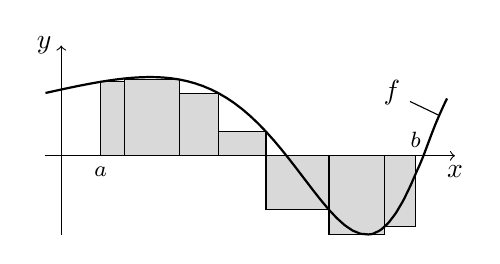
\begin{tikzpicture}
        \begin{scope}[fill = gray!30!white]
            \fill (0.5,0) -- (0.5,0.93958) -- (0.8,0.93958) -- (0.8,0) -- cycle;
            \fill (0.8,0) -- (0.8,0.968584) -- (1.5,0.968584) -- (1.5,0) -- cycle;
            \fill (1.5,0) -- (1.5,0.793203) -- (2,0.793203) -- (2,0) -- cycle;
            \fill (2,0) -- (2,0.30732) -- (2.6,0.30732) -- (2.6,0) -- cycle;
            \fill (2.6,0) -- (2.6,-0.684998) -- (3.4,-0.684998) -- (3.4,0) -- cycle;
            \fill (3.4,0) -- (3.4,-1) -- (4.1,-1) -- (4.1,0) -- cycle;
            \fill (4.1,0) -- (4.1,-0.903564) -- (4.5,-0.903564) -- (4.5,0) -- cycle;
        \end{scope}
        \draw[->] (-0.2,0) -- (5,0) node[below] {$x$};
        \draw[->] (0,-1) -- (0,1.4) node[left] {$y$};
        \draw[style = thick] plot[smooth, tension = 1] coordinates {(-0.2,0.797486) (-0.1,0.819644) (0,0.841471) (0.1,0.862814) (0.2,0.883502) (0.3,0.903341) (0.4,0.922115) (0.5,0.93958) (0.6,0.95547) (0.7,0.969487) (0.8,0.981305) (0.9,0.990566) (1,0.996883) (1.1,0.999836) (1.2,0.998975) (1.3,0.99382) (1.4,0.983866) (1.5,0.968584) (1.6,0.947432) (1.7,0.919857) (1.8,0.88531) (1.9,0.843258) (2,0.793203) (2.1,0.734701) (2.2,0.667386) (2.3,0.591003) (2.4,0.505444) (2.5,0.410781) (2.6,0.30732) (2.7,0.195643) (2.8,0.0766632) (2.9,-0.0483218) (3,-0.177577) (3.1,-0.308885) (3.2,-0.439505) (3.3,-0.566151) (3.4,-0.684998) (3.5,-0.791713) (3.6,-0.881535) (3.7,-0.94941) (3.8,-0.990193) (3.9,-0.998922) (4,-0.971185) (4.1,-0.903564) (4.2,-0.794163) (4.3,-0.64319) (4.4,-0.453553) (4.5,-0.231421) (4.6,0) (4.7,0.267039) (4.8,0.512225) (4.9,0.728508)};
        \draw (0.5,0) -- (0.5,0.93958) -- (0.8,0.93958);
        \draw (1.5,0) -- (1.5,0.968584) -- (0.8,0.968584) -- (0.8,0);
        \draw (2,0) -- (2,0.793203) -- (1.5,0.793203);
        \draw (2.6,-0.684998) -- (2.6,0.30732) -- (2,0.30732);
        \draw (3.4,-0.684998) -- (2.6,-0.684998);
        \draw (4.1,0) -- (4.1,-1) -- (3.4,-1) -- (3.4,0);
        \draw (4.1,-0.903564) -- (4.5,-0.903564) -- (4.5,0);
        \begin{scope}[every node/.append style = {font = \footnotesize}]
            \node at (0.5,-0.2) {$a$};
            \node at (4.5,0.2) {$b$};
        \end{scope}
        \node (f) at (4.2,0.8) {$f$};
        \draw (4.8,0.512225) -- (f);
    \end{tikzpicture}
    }
    \qquad
    \subfigure{
    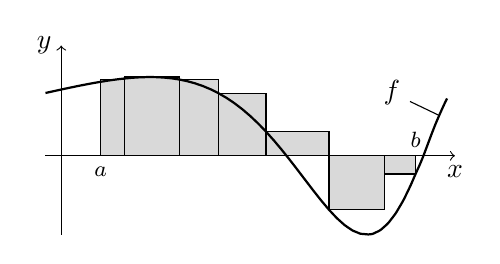
\begin{tikzpicture}
        \begin{scope}[fill = gray!30!white]
            \fill (0.5,0) -- (0.5,0.968584) -- (0.8,0.968584) -- (0.8,0) -- cycle;
            \fill (0.8,0) -- (0.8,1) -- (1.5,1) -- (1.5,0) -- cycle;
            \fill (1.5,0) -- (1.5,0.968584) -- (2,0.968584) -- (2,0) -- cycle;
            \fill (2,0) -- (2,0.793203) -- (2.6,0.793203) -- (2.6,0) -- cycle;
            \fill (2.6,0) -- (2.6,0.30732) -- (3.4,0.30732) -- (3.4,0) -- cycle;
            \fill (3.4,0) -- (3.4,-0.684998) -- (4.1,-0.684998) -- (4.1,0) -- cycle;
            \fill (4.1,0) -- (4.1,-0.231421) -- (4.5,-0.231421) -- (4.5,0) -- cycle;
        \end{scope}
        \draw[->] (-0.2,0) -- (5,0) node[below] {$x$};
        \draw[->] (0,-1) -- (0,1.4) node[left] {$y$};
        \draw[style = thick] plot[smooth, tension = 1] coordinates {(-0.2,0.797486) (-0.1,0.819644) (0,0.841471) (0.1,0.862814) (0.2,0.883502) (0.3,0.903341) (0.4,0.922115) (0.5,0.93958) (0.6,0.95547) (0.7,0.969487) (0.8,0.981305) (0.9,0.990566) (1,0.996883) (1.1,0.999836) (1.2,0.998975) (1.3,0.99382) (1.4,0.983866) (1.5,0.968584) (1.6,0.947432) (1.7,0.919857) (1.8,0.88531) (1.9,0.843258) (2,0.793203) (2.1,0.734701) (2.2,0.667386) (2.3,0.591003) (2.4,0.505444) (2.5,0.410781) (2.6,0.30732) (2.7,0.195643) (2.8,0.0766632) (2.9,-0.0483218) (3,-0.177577) (3.1,-0.308885) (3.2,-0.439505) (3.3,-0.566151) (3.4,-0.684998) (3.5,-0.791713) (3.6,-0.881535) (3.7,-0.94941) (3.8,-0.990193) (3.9,-0.998922) (4,-0.971185) (4.1,-0.903564) (4.2,-0.794163) (4.3,-0.64319) (4.4,-0.453553) (4.5,-0.231421) (4.6,0) (4.7,0.267039) (4.8,0.512225) (4.9,0.728508)};
        \draw (0.5,0) -- (0.5,0.968584) -- (0.8,0.968584);
        \draw (0.8,0) -- (0.8,1) -- (1.5,1) -- (1.5,0);
        \draw (2,0) -- (2,0.968584) -- (1.5,0.968584);
        \draw (2.6,0) -- (2.6,0.793203) -- (2,0.793203);
        \draw (3.4,-0.684998) -- (3.4,0.30732) -- (2.6,0.30732);
        \draw (4.1,0) -- (4.1,-0.684998) -- (3.4,-0.684998);
        \draw (4.5,0) -- (4.5,-0.231421) -- (4.1,-0.231421);
        \begin{scope}[every node/.append style = {font = \footnotesize}]
            \node at (0.5,-0.2) {$a$};
            \node at (4.5,0.2) {$b$};
        \end{scope}
        \node (f) at (4.2,0.8) {$f$};
        \draw (4.8,0.512225) -- (f);
    \end{tikzpicture}
    }
    \caption{구간 $[a,\,b]$에서의 분할 $\mathcal{P}$에 대한 함수 $f$의 하합 $L(f,\,\mathcal{P})$ (오른쪽)와 상합 $U(f,\,\mathcal{P})$ (왼쪽).}
\end{figure}

\begin{lemma}\label{lem:ReimannIntegrable}
    임의의 $i\leq n$와 임의의 $x_0\in\mathbb{R}$에 대해 $\mathbb{R}^n$에 속하는 초평면 $\pi:x_i=x_0$는 영집합이다.
\end{lemma}

\begin{proof}
    우선 $\pi$가 닫힌집합이므로 \texttt{Borel}이고, 따라서 이는 가측이다. 한편, \texttt{Lebesgue} 측도가 이동 불변성을 가지므로 $x_i=0$인 경우에 대해서만 증명하는 것으로 충분하고, 간결한 논의를 위해 $i=1$인 경우에 대해서만 보이도록 하자. (다른 경우에도 이와 비슷하게 보일 수 있다.) 이제 임의의 $\epsilon>0$을 택하고 집합열 $\{A_i\}$를 $A_i=(-\epsilon/2^{i+n}i^{n-1},\,\epsilon/2^{i+n}i^{n-1}]\times(-i,\,i]^{n-1}$로 두면 이는 $\mathcal{S}_n$에 속하는 집합열로서 각 $i\in\mathbb{N}$에 대해 $\lambda_n(A_i)=\epsilon/2^i$이고 $\pi\subseteq\bigcup_{i=1}^\infty A_i$이다. 이로부터 $\lambda_n(\pi)\leq\lambda_n(\bigcup_{i=1}^\infty A_i)\leq\sum_{i=1}^\infty\lambda_n(A_i)=\epsilon$이 되어 보조정리가 성립한다.
\end{proof}

\begin{theorem}\label{thm:ReimannIntegrable}
    유계인 함수 $f:\mathbb{R}^n\to\mathbb{R}$와 유계인 집합 $A\in\mathcal{M}_n$에 대해 만약 $f$가 $A$ 위에서 \texttt{Riemann} 적분가능하다면 $f\ind_A$는 \texttt{Lebesgue} 적분가능하며, 이때의 두 적분은 서로 일치한다. 즉, $\int_Af=\int_{\mathbb{R}^n}f\ind_A\,d\lambda_n$이다.
\end{theorem}

\begin{proof}
    먼저 $A$가 닫힌 \texttt{box}이고 $f$가 음이 아닌 특별한 경우를 생각하여 $A$의 임의의 분할 $\mathcal{P}$에 대해 단순함수 $\varphi_\mathcal{P},\,\psi_\mathcal{P}:\mathbb{R}^n\to\mathbb{R}^+_0$를 각각 $\varphi_\mathcal{P}=\sum_{P\in\mathcal{P}}\inf_{x\in P}f(x)\ind_{\widetilde{P}},\,\psi_\mathcal{P}=\sum_{P\in\mathcal{P}}\sup_{x\in P}f(x)\ind_{\widetilde{P}}$로 두자. (여기서 $\widetilde{P}$는 box $P$의 남서쪽 면을 빼서 얻는 \texttt{semi-open box}로서 적당한 $x,\,y\in\mathbb{R}^n$에 대해 $P=[x,\,y]$라면 $\widetilde{P}=(x,\,y]$이다.) 그렇다면
    \begin{align*}
        \int_{\mathbb{R}^n}\varphi_\mathcal{P}\,d\lambda_n&=\sum_{P\in\mathcal{P}}\inf_{x\in P}f(x)\int_{\mathbb{R}^n}\ind_{\widetilde{P}}\,d\lambda_n\\
        &=\sum_{P\in\mathcal{P}}\inf_{x\in P}f(x)\lambda_n(\widetilde{P})\\
        &=\sum_{P\in\mathcal{P}}\inf_{x\in P}f(x)\vol(P)\\
        &=L(f,\,\mathcal{P})
    \end{align*}
    이고 비슷하게 $\int_{\mathbb{R}^n}\psi_\mathcal{P}\,d\lambda_n=U(f,\,\mathcal{P})$이다. 이제 $f$가 $A$위에서 \texttt{Riemann} 적분가능하므로 임의의 $i\in\mathbb{N}$에 대해 적당한 $A$의 분할 $\mathcal{P}_i$가 존재하여 $U(f,\,\mathcal{P}_i)-L(f,\,\mathcal{P}_i)<1/i$이고, 이들을 모아 분할의 열 $\{\mathcal{P}_i\}$를 구성할 수 있고, \texttt{WLOG}, 필요하다면 각 항을 $\mathcal{Q}_i:=\bigcup_{j=1}^i\mathcal{P}_j$로 바꾸어 $\{\mathcal{P}_i\}$가 처음부터 증가했다고 해도 된다. 그렇다면 $\{\varphi_{\mathcal{P}_i}\},\,\{\psi_{\mathcal{P}_i}\}$는 각각 증가하고 감소하는 함수열로 $\{\psi_{\mathcal{P}_i}-\varphi_{\mathcal{P}_i}\}$가 감소하는 음이 아닌 함수열이 되어 이가 모든 점에서 수렴하고, 곧 \texttt{Fatou}의 보조정리로부터
    \begin{align*}
        \int_{\mathbb{R}^n}\lim_{i\to\infty}(\psi_{\mathcal{P}_i}-\varphi_{\mathcal{P}_i})\,d\lambda_n&\leq\liminf_{i\to\infty}\int_{\mathbb{R}^n}\psi_{\mathcal{P}_i}-\varphi_{\mathcal{P}_i}\,d\lambda_n\\
        &=\lim_{i\to\infty}\bigg(\int_{\mathbb{R}^n}\psi_{\mathcal{P}_i}\,d\lambda_n-\int_{\mathbb{R}^n}\varphi_{\mathcal{P}_i}\,d\lambda_n\bigg)\\
        &=\lim_{i\to\infty}[U(f,\,\mathcal{P}_i)-L(f,\,\mathcal{P}_i)]\\
        &=0
    \end{align*}
    이다. 이는 정리 \ref{thm:zeroAeIntegral}의 ii로부터 $\psi_{\mathcal{P}_i}-\varphi_{\mathcal{P}_i}\downarrow0$ (\texttt{ae.})임을 뜻하고, 특히 위의 보조정리로부터 모든 $i\in\mathbb{N}$에 대해 $\varphi_{\mathcal{P}_i}\leq f\ind_A\leq\psi_{\mathcal{P}_i}$ (\texttt{ae.})가 성립하므로\footnotemark $\varphi_{\mathcal{P}_i}\uparrow f\ind_A$ (\texttt{ae.})가 되어 정리 \ref{thm:limitAeMeasurable}로부터 $f\ind_A$가 가측임을 안다. 이제 \texttt{MCT}로부터 $\int_{\mathbb{R}^n}f\ind_A\,d\lambda_n=\lim_{i\to\infty}\int_{\mathbb{R}^n}\varphi_{\mathcal{P}_i}\,d\lambda_n=\lim_{i\to\infty} U(f,\,\mathcal{P}_i)=\int_Af<\infty$이므로 $f\ind_A$는 \texttt{Lebesgue} 적분가능하고 두 적분이 일치한다.

    한편, 일반적인 경우에 대해서는 $A\subseteq B\in\mathbb{R}^n$인 임의의 닫힌 \texttt{box} $B$를 잡으면 이전의 결과로부터
    \begin{align*}
        \int_{\mathbb{R}^n}f\ind_A\,d\lambda_n&=\int_{\mathbb{R}^n}(f\ind_A)_+\,d\lambda_n-\int_{\mathbb{R}^n}(f\ind_A)_-\,d\lambda_n\\
        &=\int_{\mathbb{R}^n}f_+\ind_A\ind_B\,d\lambda_n-\int_{\mathbb{R}^n}f_-\ind_A\ind_B\,d\lambda_n\\
        &=\int_Bf_+\ind_A-\int_Bf_-\ind_A\\
        &=\int_Af_+-\int_Af_-\\
        &=\int_Af
    \end{align*}
    이고, 곧 일반적인 경우에도 $f\ind_A$는 \texttt{Lebesgue} 적분가능하며 두 적분이 일치한다.
\end{proof}

\begin{definition}
    유계인 음이 아닌 함수 $f:\mathbb{R}^n\to\mathbb{R}^+_0$와 집합 $A\in\mathcal{M}_n$에 대해 $f\ind_A$가 적당한 $x>0$에 대해 $[-x,\,x]^n$으로 표현되는 모든 닫힌 \texttt{box} 위에서 \texttt{Riemann} 적분가능하다고 하자. 만약 $\lim_{x\to\infty}\int_{[-x,\,x]^n}f\ind_A<\infty$이면 이때 $f$가 \textbf{$A$ 위에서 (\texttt{Riemann}) 적분가능(- \texttt{integrable over} $A$)}하다고 하고, 그 극한을 $\int_Af(x)\,dx$ 혹은 간단히 $\int_Af$로 쓴다. 나아가, 함수 $f:\mathbb{R}^n\to\mathbb{R}$에 대해서는 $f_\pm$이 모두 $A$ 위에서 \texttt{Riemann} 적분가능하다면 이때 $f$가 \textbf{$A$ 위에서 (\texttt{Riemann}) 적분가능(- \texttt{integrable over} $A$)}하다고 하고, $\int_Af_+-\int_Af_-$의 값을 $\int_Af(x)\,dx$ 혹은 간단히 $\int_Af$로 쓴다.
\end{definition}

\begin{theorem}\label{thm:ReimannIntegrable2}
    유계인 함수 $f:\mathbb{R}^n\to\mathbb{R}$와 집합 $A\in\mathcal{M}_n$에 대해 만약 $f$가 $A$ 위에서 \texttt{Riemann} 적분가능하다면 $f\ind_A$는 \texttt{Lebesgue} 적분가능하며, 이때의 두 적분은 서로 일치한다. 즉, $\int_Af=\int_{\mathbb{R}^n}f\ind_A\,d\mu$이다.
\end{theorem}

\begin{proof}
    함수 $f_i:\mathbb{R}^n\to\mathbb{R}$의 열 $\{f_i\}$를 $f_i=f\ind_{A\cap[-i,\,i]^n}$으로 정의하면 이는 유계함수열이고 $f_i\to f\ind_A$인데 각 $i\in\mathbb{N}$에 대해 $f_i$가 $[-i,\,i]^n$ 위에서 \texttt{Riemann} 적분가능하므로 정리 \ref{thm:ReimannIntegrable}로부터 가측이고, 곧 정리 \ref{thm:limitAeMeasurable}로부터 $f\ind_A$도 가측이다. 이제 $f$가 음이 아닌 특별한 경우를 생각하면 \texttt{WLOG}, $\{f_i\}$가 증가한다고 할 수 있다. 그렇다면 \texttt{MCT}와 정리 \ref{thm:ReimannIntegrable}로부터 $\int_{\mathbb{R}^n}f\ind_A\,d\lambda_n=\lim_{i\to\infty}\int_{\mathbb{R}^n}f_i\,d\lambda_n=\lim_{i\to\infty}\int_{[-i,\,i]^n}f\ind_A=\int_Af<\infty$가 되어 $f\ind_A$는 \texttt{Lebesgue} 적분가능하고 두 적분이 일치한다. 한편, 일반적인 $f$에 대해서는 
    \begin{align*}
        \int_{\mathbb{R}^n}f\ind_A\,d\lambda_n&=\int_{\mathbb{R}^n}(f\ind_A)_+\,d\lambda_n-\int_{\mathbb{R}^n}(f\ind_A)_-\,d\lambda_n\\
        &=\int_{\mathbb{R}^n}f_+\ind_A\,d\lambda_n-\int_{\mathbb{R}^n}f_-\ind_A\,d\lambda_n\\
        &=\int_Af_+-\int_Af_-\\
        &=\int_Af
    \end{align*}
    이므로 이때에도 같은 결론이 성립한다.
\end{proof}

\begin{definition}
    음이 아닌 함수 $f:\mathbb{R}^n\to\mathbb{R}^+_0$와 집합 $A\in\mathcal{M}_n$, 충분히 큰 $M\in\mathbb{R}$에 대해 $f_{(M)}:=\min\{f,\,M\}$이 $A$ 위에서 \texttt{Riemann} 적분가능하다고 하자. 만약 $\lim_{M\to\infty}\int_Af_{(M)}<\infty$이면 이때 $f$가 \textbf{$A$ 위에서 (\texttt{Riemann}) 적분가능(- \texttt{integrable over} $A$)}하다고 하고, 그 극한을 $\int_Af(x)\,dx$ 혹은 간단히 $\int_Af$로 쓴다. 나아가, 유계인 함수 $f:\mathbb{R}^n\to\mathbb{R}$에 대해서는 $f_\pm$이 모두 $A$ 위에서 \texttt{Riemann} 적분가능하다면 이때 $f$가 \textbf{$A$ 위에서 (\texttt{Riemann}) 적분가능(- \texttt{integrable over} $A$)}하다고 하고, $\int_Af_+-\int_Af_-$의 값을 $\int_Af(x)\,dx$ 혹은 간단히 $\int_Af$로 쓴다.
\end{definition}

\begin{figure}[!ht]
    \sidecaption[b]
    \centering
    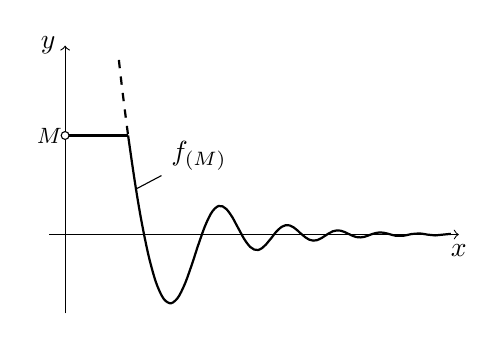
\begin{tikzpicture}
        \draw[->] (-0.2,0) -- (5,0) node[below] {$x$};
        \draw[->] (0,-1) -- (0,2.4) node[left] {$y$};
        \begin{scope}[style = thick]
            \clip (-0.2,-1) -- (-0.2,2.3) -- (5,2.3) -- (5,-1) -- cycle;
            \draw[style = dashed] plot[smooth, tension = 0.7] coordinates{(0.1,30.038) (0.2,14.0557) (0.3,8.70459) (0.4,5.97429) (0.5,4.25995) (0.6,3.02927) (0.7,2.06151) (0.8,1.25777)};
            \draw plot[smooth, tension = 0.7] coordinates {(0.8,1.25777) (0.9,0.577741) (1,0.0133254) (1.1,-0.425578) (1.2,-0.721688) (1.3,-0.860253) (1.4,-0.83866) (1.5,-0.674437) (1.6,-0.409227) (1.7,-0.106062) (1.8,0.161646) (1.9,0.328402) (2,0.357505) (2.1,0.256506) (2.2,0.0785027) (2.3,-0.0956905) (2.4,-0.190957) (2.5,-0.173249) (2.6,-0.067714) (2.7,0.0545424) (2.8,0.118369) (2.9,0.0919484) (3,0.00718648) (3.1,-0.0652574) (3.2,-0.0714696) (3.3,-0.0170933) (3.4,0.0408613) (3.5,0.0488495) (3.6,0.00761784) (3.7,-0.0326739) (3.8,-0.0293643) (3.9,0.00622508) (4,0.0268959) (4.1,0.0101463) (4.2,-0.0159768) (4.3,-0.0151862) (4.4,0.00646553) (4.5,0.0141145) (4.6,-0.000966882) (4.7,-0.0112569) (4.8,-0.00127191) (4.9,0.00862194)};
            \draw (0,1.25777) -- (0.8,1.25777);
        \end{scope}
        \draw[fill = white] (0,1.25777) circle[radius = 0.05];
        \begin{scope}[every node/.append style = {font = \footnotesize}]
            \node at (-0.2,1.25777) {$M$};
        \end{scope}
        \node (f) at (1.7,1) {$f_{(M)}$};
        \draw (0.9,0.577741) -- (f);
    \end{tikzpicture}
    \caption{함수 $f$ (파선)에 대한 $f_{(M)}$의 그래프. 여기서 $f$는 $x\downarrow 0$이면 $\infty$로 발산한다.}
\end{figure}

\begin{theorem}
    함수 $f:\mathbb{R}^n\to\mathbb{R}$와 집합 $A\in\mathcal{M}_n$에 대해 만약 $f$가 $A$ 위에서 \texttt{Riemann} 적분가능하다면 $f\ind_A$는 \texttt{Lebesgue} 적분가능하며, 이때의 두 적분은 서로 일치한다. 즉, $\int_Af=\int_{\mathbb{R}^n}f\ind_A\,d\mu$이다.
\end{theorem}

\begin{proof}
    함수 $f_i:\mathbb{R}^n\to\mathbb{R}$의 열 $\{f_i\}$를 $f_i=f_{(i)}\ind_A$로 정의하면 이는 증가하는 유계함수열이고 $f_i\uparrow f\ind_A$인데 충분히 큰 $i\in\mathbb{N}$에 대해 $f_i$가 $A$ 위에서 \texttt{Riemann} 적분가능하므로 정리 \ref{thm:ReimannIntegrable2}로부터 가측이고, 곧 정리 \ref{thm:limitAeMeasurable}로부터 $f\ind_A$도 가측이다. 여기서 \texttt{WLOG}, $f_i$가 모든 $i\in\mathbb{N}$에 대해 \texttt{Riemann} 적분가능하다고 하자. 이제 $f$가 음이 아닌 특별한 경우를 생각하면 \texttt{MCT}와 정리 \ref{thm:ReimannIntegrable2}로부터 $\int_{\mathbb{R}^n}f\ind_A\,d\lambda_n=\lim_{i\to\infty}\int_{\mathbb{R}^n}f_i\,d\lambda_n=\lim_{i\to\infty}\int_Af_{(i)}=\int_Af<\infty$가 되어 $f\ind_A$는 \texttt{Lebesgue} 적분가능하고 두 적분이 일치한다. 한편, 일반적인 $f$에 대해서는
    \begin{align*}
        \int_{\mathbb{R}^n}f\ind_A\,d\lambda_n&=\int_{\mathbb{R}^n}(f\ind_A)_+\,d\lambda_n-\int_{\mathbb{R}^n}(f\ind_A)_-\,d\lambda_n\\
        &=\int_{\mathbb{R}^n}f_+\ind_A\,d\lambda_n-\int_{\mathbb{R}^n}f_-\ind_A\,d\lambda_n\\
        &=\int_Af_+-\int_Af_-\\
        &=\int_Af
    \end{align*}
    이므로 이때에도 같은 결론이 성립한다.
\end{proof}

따라서 다행히도 \texttt{Lebesgue} 적분은 \texttt{Riemann} 적분을 포괄하는 개념으로, 이론 전개를 할 때는 \texttt{Lebesgue} 적분으로 생각하여 이론을 전개하고, 실제로 계산을 해야 할 때에는 이를 \texttt{Riemann} 적분으로 생각하여 \texttt{FTC} 등을 사용해 계산해도 대부분의 경우 문제가 없다. 다만, 여기서도 조심해야 할 부분이 있는데, 바로 \texttt{improper}한 \texttt{Riemann} 적분은 이가 절대수렴하는 경우에만 \texttt{Lebesgue} 적분과 그 값이 일치한다는 것이다. \texttt{Riemann} 적분이 조건수렴에 그치는 $\int_0^\infty(\sin x)/x\,dx$와 같은 경우 이의 \texttt{Lebesgue} 적분가능성은 일반적으로 보장되지 않는다. 물론, 이 책에서는 조건수렴에 그치는 \texttt{Riemann} 적분을 다룰 일이 (아마) 없을 것이므로 안심해도 좋다.

\section{$L^p$ Space and Radon-Nikod\'ym Theorem}

지금까지 우리는 측도라는 개념으로 넓이나 부피 따위를 일반화하였고, 이를 이용하여 \texttt{Lebesgue} 적분의 개념을 정립함으로써 $\mathbb{R}^n$에서 뿐만 아니라 측도가 주어진 임의의 공간에서 적분을 할 수 있는 이론적 토대를 마련하였다. 이번 절에서는 이런 추상화의 흐름에 발맞추어 적분의 역연산인 미분의 개념을 임의의 공간으로 확장하려고 한다. 한편, 이를 위해서는 $L^p$ 공간이라는 경유지가 필요한데, $L^p$ 공간은 그 자체로도 꽤나 흥미로운 탐구의 대상이어서 파고들자면 끝도 없으므로 여기서는 우리에게 필요한 정도만 선택적으로 그 내용을 소개하도록 하겠다. 이에 대해 조금 더 관심이 있는 독자들은 [2]와 같은 실해석학 교재를 고조하기 바란다.

\begin{definition}
    측도공간 $(X,\,\mathcal{A},\,\mu)$에서 정의된 가측함수 $f:X\to\overline{\mathbb{R}}$와 $p\geq1$에 대해 $(\int_X|f|^p\,d\mu)^{1/p}$를 $f$의 \textbf{$p$-노름($p$-\texttt{norm})}이라 하고 $||f||_{p,\,\mu}$ 혹은 간단히 $||f||_p$로 쓴다.
\end{definition}

\begin{proposition}\label{prop:lpnormScale}
    측도공간 $(X,\,\mathcal{A},\,\mu)$에서 정의된 가측함수 $f:X\to\overline{\mathbb{R}}$와 $p\geq1$에 대해 다음이 성립한다.
    \begin{enumerate}
        \item 임의의 $\lambda\in\mathbb{R}$에 대해 $||\lambda f||_p=|\lambda|||f||_p$이다.
        \item $||f||_p=0$일 필요충분조건은 $f=0$ (\texttt{ae.})이다.
    \end{enumerate}
\end{proposition}

\begin{proof}
    i. 이는 $||\lambda f||_p=(\int_X|\lambda f|^p\,d\mu)^{1/p}=|\lambda|(\int_X|f|^p\,d\mu)^{1/p}=|\lambda|||f||_p$에서 자명하다.

    ii. $\int_X|f|^p\,d\mu=||f||_p^p=0$이므로 정리 \ref{thm:zeroAeIntegral}의 ii로부터  $|f|=0$ (\texttt{ae.})이고, 곧 $f=0$ (\texttt{ae.})이다. 한편, 역은 자명하다.
\end{proof}

\begin{theorem}[H\"older's inequality]\label{thm:holderIneq}
    측도공간 $(X,\,\mathcal{A},\,\mu)$에서 정의된 가측함수 $f,\,g:X\to\overline{\mathbb{R}}$와 $1/p+1/q=1$인 $p,\,q>1$에 대해 $\int_X|fg|\,d\mu\leq||f||_p||g||_q$이다. 이때, $||f||_p,\,||g||_q<\infty$라면 등호가 성립할 필요충분조건은 모두 $0$은 아닌 적당한 $a,\,b\in\mathbb{R}$가 존재하여 $a|f|^p+b|g|^q=0$ (\texttt{ae.})인 것이다.
\end{theorem}

\begin{proof}
    \texttt{WLOG}, 필요하다면 $f,\,g$를 각각 $|f|,\,|g|$로 대체하여 $f,\,g$가 처음부터 음이 아니라 해도 된다. 한편, 만약 $||f||_p=0$이면 명제 \ref{prop:lpnormScale}의 ii로부터 $f=0$ (\texttt{ae.})이고, 곧 $\int_X|fg|\,d\mu=0$이 되어 부등식이 자명하므로 $||f||_p>0$이라 하고, 비슷한 이유로 $||g||_p>0$이라 하자. 또한 $||f||_p=\infty$이거나 $||g||_p=\infty$인 경우에도 부등식이 자명하므로 $||f||_p,\,||g||_p<\infty$라 하자. 이제 $||f||_p=||g||_q=1$인 특별한 경우를 생각하면 \texttt{Young}의 부등식으로부터 $\int_Xfg\,d\mu\leq\int_Xf^p/p+g^q/q\,d\mu=||f||_p^p/p+||g||_q^q/q=1/p+1/q=1$이다. 이어서 일반적인 경우에 $\widetilde{f}=f/||f||_p,\,\widetilde{g}=g/||g||_q$라 하면 명제 \ref{prop:lpnormScale}의 i로부터 $||\widetilde{f}||_p=||\widetilde{g}||_q=1$이므로 앞선 결과로부터 $\int_X|\widetilde{f}\widetilde{g}|\,d\mu\leq1$이 되어 곧 $\int_X|fg|\,d\mu\leq||f||_p||g||_q$임을 안다.

    다음으로, 등호조건을 보이기 위해 $||f||_p,\,||g||_q<\infty$이고 $\int_X|fg|\,d\mu=||f||_p||g||_q$라 하자. 만약 $||f||_p=0$이면 $f=0$ (\texttt{ae.})에서 $|f|^p+0\cdot|g|^q=0$ (\texttt{ae.})가 되어 더 이상 보일 것이 없으므로 $||f||_p\ne0$이라 하고, 비슷한 이유에서 $||g||_q\ne0$이라 하자. 이제 $\widetilde{f}=|f|/||f||_p,\,\widetilde{g}=|g|/||g||_q$라 하면 $\int_X\widetilde{f}\widetilde{g}\,d\mu=(\int_X|fg|\,d\mu)/||f||_p||g||_q=1=||\widetilde{f}||_p^p/p+||\widetilde{g}||_q^q/q=\int_X\widetilde{f}^p/p+\widetilde{g}^q/q\,d\mu$이므로 \texttt{Young}의 부등식과 정리 \ref{thm:zeroAeIntegral}의 ii로부터 $\widetilde{f}\widetilde{g}=\widetilde{f}^p/p+\widetilde{g}^q/q$ (\texttt{ae.})이다. 이는 다시 \texttt{Young}의 부등식의 등호조건으로부터 $\widetilde{f}^p=\widetilde{g}^q$ (\texttt{ae.})를 뜻하고, 따라서 $||g||_q^q|f|^p-||f||_p^p|g|^q=0$ (\texttt{ae.})이다. 역으로 모두 $0$은 아닌 적당한 $a,\,b\in\mathbb{R}$가 존재하여 $a|f|^p+b|g|^q=0$ (\texttt{ae.}) 경우에 등호가 성립함은 자명하므로 증명은 이로써 충분한다.
\end{proof}

\begin{theorem}[Minkowski's inequality]
    측도공간 $(X,\,\mathcal{A},\,\mu)$에서 정의된 가측함수 $f,\,g:X\to\overline{\mathbb{R}}$와 $p\geq1$에 대해 $||f+g||_p\leq||f||_p+||g||_p$이다. 이때, $||f||_p,\,||g||_p<\infty$이면 등호가 성립한 필요충분조건은 모두 $0$은 아닌 적당한 $a,\,b\in\mathbb{R}$가 존재하여 $a|f|^p+b|g|^p=0$ (\texttt{ae}.)인 것이다.
\end{theorem}

\begin{proof}
    만약 $p=1$이면 $||f+g||_1=\int_X|f+g|\,d\mu\leq\int_X|f|\,d\mu+\int_X|g|\,d\mu=||f||_1+||g||_1$에서 부등식이 자명하므로 $p>1$이라 하자. 또한, 만약 $||f||_p=\infty$이거나 $||g||_p=\infty$이거나 $||f+g||_p=0$인 경우에도 부등식이 자명하므로 $||f||_p,\,||g||_p<\infty$이고 $||f+g||_p>0$이라 하자. 그렇다면 $|f|,\,|g|\leq(|f|^p+|g|^p)^{1/p}$이므로 $|f+g|^p\leq(|f|+|g|)^p\leq2^p(|f|^p+|g|^p)$에서 $\int_X|f+g|^p\,d\mu\leq2^p\int_X|f|^p+|g|^p\,d\mu=2^p(||f||_p^p+||g||_p^p)<\infty$이고, 곧 $||f+g||_p<\infty$이다. 따라서 \texttt{H\"older}의 부등식으로부터 $1/p+1/q=1$인 $q>1$에 대해
    \begin{align*}
        ||f+g||_p^p&=\int_X|f+g|^p\,d\mu\\
        &\leq\int_X|f||f+g|^{p-1}\,d\mu+\int_X|g||f+g|^{p-1}\,d\mu\\
        &\leq||f||_p|||f+g|^{p-1}||_q+||g||_p|||f+g|^{p-1}||_q\\
        &=(||f||_p+||g||_p)\bigg(\int_X|f+g|^{(p-1)q}\,d\mu\bigg)^{1/q}\\
        &=(||f||_p+||g||_p)\bigg(\int_X|f+g|^p\,d\mu\bigg)^{(p-1)/p}\\
        &=(||f||_p+||g||_p)||f+g||_p^{p-1}
    \end{align*}
    이 성립하여 $||f+g||_p\leq||f||_p+||g||_p$임을 안다.

    다음으로, 등호조건을 보이기 위해 $||f||_p,\,||g||_p<\infty$이고 $||f+g||_p=||f||_p+||g||_p$라 하자. 만약 $f=0$ (\texttt{ae}.)이면 $|f|^p+0\cdot|g|^p=0$ (\texttt{ae}.)에서 더 이상 보일 것이 없으므로 $f=0$ (\texttt{ae}.)이 아니라 하고, 비슷한 이유에서 $g=0$ (\texttt{ae}.)도 아니라 하자. 그렇다면 위의 증명과정과 \texttt{H\"older}의 부등식의 등호조건으로부터 적당한 $a_1,\,a_2,\,b_1,\,b_2\in\mathbb{R}$가 존재하여 $a_1|f|^p+b_2|f+g|^{(p-1)q}=a_1|f|^p+b_2|f+g|^p=0$ (\texttt{ae}.)이고 $a_2|g|^p+b_2|f+g|^{(p-1)q}=a_2|g|^p+b_2|f+g|^p=0$ (\texttt{ae}.)이다. 여기서 만약 $a_1=0$이면 $f+g=0$ (\texttt{ae}.)가 되어 $||f||_p+||g||_p=||f+g||_p=0$에서 $f=g=0$ (\texttt{ae}.)의 모순이 발생하므로 $a_1\ne0$이고 $b_1=0$이면 $f=0$ (\texttt{ae}.)의 모순이 발생하므로 $b_1\ne0$이다. 비슷하게 $a_2,\,b_2\ne0$이므로 이상을 종합하면 $a_1b_2|f|^p-a_2b_1|g|^p$ (\texttt{ae}.)이고 $a_1b_2,\,a_2b_1\ne0$이다. 역으로 모두 $0$은 아닌 적당한 $a,\,b\in\mathbb{R}$가 존재하여 $a|f|^p+b|g|^p=0$ (\texttt{ae}.)인 경우에 등호가 성립함은 자명하므로 증명은 이로써 충분하다.
\end{proof}

당장은 $p$-노름은 노름이 아니라는 점에 주의하자. 명제 \ref{prop:lpnormScale}의 i과 \texttt{Minkowski}의 부등식으로부터 $p$-노름이 양의 동차성과 삼각부등식은 만족하지만, 아직 이가 양의 정부호성을 만족하는지는 알지 못한다. 그리고 조금만 생각해보면, $p$-노름이 양의 정부호성을 갖길 기대하는 건 부질없는 것임을 깨달을 수 있다. 적분값이 0이라고 해서 피적분함수가 반드시 0일 필요는 없기 때문이다. 그럼에도 이에 $p$-노름이라는 이름을 괜히 붙인 것은 아닐테니, $p$-노름을 정말 노름으로 만들기 위해서는 `도약'이 필요하다.

\begin{definition}
    측도공간 $(X,\,\mathcal{A},\,\mu)$에서 정의된 가측함수 $f:X\to\overline{\mathbb{R}}$와 $p\geq1$에 대해 만약 $||f||_p<\infty$이면 이를 \textbf{$L^p(\mu)$-함수($L^p(\mu)$-\texttt{function})} 혹은 간단히 \textbf{$L^p$-함수($L^p$-\texttt{function})}라 한다. 나아가, $X$에서 정의된 모든 $L^p$-함수의 모임을 $\mathcal{L}^p(\mu)$ 혹은 간단히 $\mathcal{L}^p$로 쓴다.
\end{definition}

\begin{definition}
    측도공간 $(X,\,\mathcal{A},\,\mu)$와 $p\geq1$에 대해 $\mathcal{L}^p(\mu)$ 위의 동치관계 $\musim$를 $f\musim g:\Leftrightarrow f=g$ (\texttt{ae.})로 정의하고 이의 몫공간 $\mathcal{L}^p(\mu)/\musim$를 \textbf{\texttt{Lebesgue} 공간(- \texttt{space})}, \textbf{$L^p(\mu)$-공간($L^p(\mu)$-\texttt{space})} 혹은 간단히 \textbf{$L^p$-공간($L^p$-\texttt{space})}이라 하고 $L^p(\mu)$ 혹은 간단히 $L^p$로 쓴다.
\end{definition}

언듯 보아서는 뭔가 이상한 짓을 한 것 같지만 이러한 $L^p$ 공간의 구성은 굉장히 직관적인 구성이다. 앞서 보았듯이 $p$-노름이 가지는 문제점은 양의 정부호성이 성립하지 않는다는 것이었는데, 명제 \ref{prop:lpnormScale}의 ii에 의하면 $||f||_p=0$이면 $f$가 거의 어디서나 0인 것까지는 보장이 되었다. 우리는 이에 착안하여 거의 어디서나 같은 것을 정말 같은 것으로 볼 수 있는 공간을 구성한 것이다. 이제 우리의 도약은 $L^p$ 공간에 적당한 노름공간의 구조를 부여함으로써 마무리된다.

\begin{proposition}
    측도공간 $(X,\,\mathcal{A},\,\mu)$와 $p\geq1$에 대해 함수 $+:(L^p)^2\to L^p,\,\cdot:\mathbb{R}\times L^p\to L^p$를 각각 $+:([f],\,[g])\mapsto[f+g],\,\cdot:(\lambda,\,[f])\mapsto[\lambda f]$로 정의하면 $(L^p,\,+,\,\cdot,\,[0],\,1)$은 벡터공간이다.
\end{proposition}

\begin{proof}
    정리에서 정의된 덧셈과 스칼라 곱이 \texttt{well-define}된다는 것만 보이면 $(L^p,\,+,\,\cdot,\,[0],\,1)$이 벡터공간이 되기 위한 조건은 쉽게 확인할 수 있으므로 여기서는 \texttt{well-definedness}만 보이도록 하자. 이를 위해 임의의 $f,\,g\in\mathcal{L}^p$와 임의의 $\lambda\in\mathbb{R}$를 생각하면 \texttt{Minkowski}의 부등식으로부터 $||f+g||_p\leq||f||_p+||g||_p<\infty$이고 명제 \ref{prop:lpnormScale}의 i로부터 $||\lambda f||_p=|\lambda|||f||_p<\infty$이므로 $f+g,\,\lambda f\in\mathcal{L}^p$이다. 나아가, 주어진 덧셈과 스칼라 곱의 결과가 \texttt{representative}의 선택에 의존하지 않음이 자명하므로 이는 \texttt{well-define}된다.
\end{proof}

\begin{proposition}
    측도공간 $(X,\,\mathcal{A},\,\mu)$와 $p\geq1$에 대해 함수 $||\cdot||_p:L^p\to\mathbb{R}_0^+$를 $||\cdot||_p:[f]\mapsto||f||_p$로 정의하면 $(L^p,\,||\cdot||_p)$는 노름공간이다.
\end{proposition}

\begin{proof}
    우선 따름정리 \ref{cor:zeroAeIntegral}의 ii로부터 $||\cdot||_p$는 \texttt{representative}의 선택에 의존하지 않으므로 \texttt{well-define}된다. 나아가 명제 \ref{prop:lpnormScale}의 i과 \texttt{Minkowski}의 부등식으로부터 양의 동차성과 삼각부등식이 성립하고, 명제 \ref{prop:lpnormScale}의 ii와 $L^p$ 공간의 구성으로부터 이가 양의 정부호성도 가지므로 $(L^p,\,||\cdot||_p)$은 노름공간이다.
\end{proof}

보통 특별히 정하지 않는 이상 $L^p$ 공간에는 $p$-노름이 주어진 것으로 생각하고, 이는 이 책에서도 마찬가지이다. 또한, 일반적으로 노름공간 $(L^p,\,||\cdot||_p)$의 원소 $[f]$를 표기를 남용하여 그냥 $f$로 쓴다. 이렇게 집합인 동치류를 마치 함수처럼 표기하는 것에 처음에는 거부감을 느낄 수 있다. 하지만 $L^p$에서 진행되는 논의는 대부분 적분에 관한 논의이고, 곧 이러한 맥락에서는 함수의 특정 점에서의 값보다는 그 함수의 적분값이 중요한데, 거의 어디서나 같은 함수는 적어도 적분에서는 구별할 필요가 없으므로 이러한 표기법은 굉장히 편리하다. 또한, $L^p$ 공간의 기저에 깔려있는 거의 어디서나 같은 것은 정말 같다는 그 철학을 생각한다면 오히려 이러한 표기가 자연스러운 표기법이라고 생각할 수도 있다.

다만, 이러한 표기의 남용으로 인하여 $L^p$에 속하는 동치류로서 $[f]$를 뜻하는 $f$와 $[f]$의 임의의 \texttt{representative}로서 $\mathcal{L}^p$에 속하는 구체적인 함수를 뜻하는 $f$가 적어도 표기로써는 구별되지 않으므로 이를 논의의 맥락으로써 잘 구별해야 한다. 대부분의 경우, 이러한 구별은 그다지 어렵지 않다. 한 예시로 아래의 따름정리 \ref{cor:lpBanach}의 `$L^p$에 속하는 함수열 $\{f_i\}$가 적당한 $f\in L^p$에 대해 $f_i\to f$ \texttt{in sense of} $L^p$이면 $\{f_i\}$의 적당한 부분함수열이 존재하여 거의 어디서나 $f$로 수렴한다.'는 표현을 보자. 먼저 `$L^p$에 속하는 함수열 $\{f_i\}$'에서의 $f_i$는 $L^p$에 속하는 동치류로 $[f_i]$를 이르는 것이고, 이를 표기를 남용하여 $f_i$라 쓰고 그에 걸맞게 `함수열'이라 표현하였다. 이어지는 `적당한 $f\in L^p$에 대해 $f_i\to f$ \texttt{in sense of} $L^p$' 또한 동치류의 열 $\{[f_i]\}$가 $p$-노름으로써 동치류 $[f]\in L^p$로 수렴한다는 뜻으로, `\texttt{in sense of} $L^p$'라는 표현에서 그 의미가 분명하다. 한편, 끝부분의 `$\{f_i\}$의 적당한 부분함수열이 존재하여 거의 어디서나 $f$로 수렴한다'는 $[f_i]$의 임의의 \texttt{representative}를 택하여 구성한 $\mathcal{L}^p$에 속하는 (진짜) 함수열 $\{f_i\}$에 대해 적당한 부분함수열 $\{f_{i_j}\}$가 존재하여 $[f]$의 임의의 \texttt{representative} $f$로 거의 어디서나 점별수렴함을 뜻하는 것으로, 이러한 거의 어디서나 점별수렴한다는 결론이 $[f_i]$나 $[f]$의 \texttt{representative}의 선택에 의존하지 아니하므로 그 의미의 전달이 분명하다. 이와 같이 맥락에 따라 그 의미를 파악하며 읽는 것은, 처음에는 다소 시간이 걸리겠지만, 머지않아 익숙해 질 것이다.

우리는 $p$-노름이 정말 노름이 되도록 하기 위해 $L^p$ 공간을 도입했지만, $L^p$ 공간은 우리가 생각하는 것보다 훨씬 더 아름다운 공간이다. 지금부터는 $L^p$ 공간이 함수공간으로서 가지는 성질을 알아보자.

\begin{definition}
    노름공간 $(\mathsf{V},\,||\cdot||)$에 대해 $||\cdot||$이 완비성을 가지면즉 임의의 \texttt{Cauchy} 수열이 수렴하면, 이때의 $(\mathsf{V},\,||\cdot||)$를 \textbf{\texttt{Banach} 공간(- \texttt{space})}이라 한다.
\end{definition}

\begin{theorem}\label{thm:lpBanach}
    측도공간 $(X,\,\mathcal{A},\,\mu)$와 $p\geq1$에 대해 $(L^p,\,||\cdot||_p)$는 \texttt{Banach} 공간이다.
\end{theorem}

\begin{proof}
    $L^p$ 공간에 속하는 임의의 \texttt{Cauchy} 수열 $\{f_i\}$를 택하면 임의의 $j\in\mathbb{N}$에 대해 적당한 $i_j\in\mathbb{N}$가 존재하여 임의의 $i,\,i'\geq i_j$에 대해 $||f_i-f_{i'}||_p<2^{-j}$이다. \texttt{WLOG}, 필요하다면 $i_j$를 더 크게 잡음으로써 $\{i_j\}_j$를 증가수열이라 해도 되고, 이로부터 부분열 $\{f_{i_j}\}_j$를 생각하면 이는 임의의 $j\in\mathbb{N}$에 대해 $||f_{i_j}-f_{i_{j+1}}||_p<2^{-j}$인 함수열이다. 이제 함수 $g_j:X\to\overline{\mathbb{R}}$의 열 $\{g_j\}$를 $g_j=\sum_{k=1}^j|f_{i_{k+1}}-f_{i_k}|$로 정의하고 함수 $g:X\to\overline{\mathbb{R}}$를 $g=\sum_{k=1}^\infty|f_{i_{k+1}}-f_{i_k}|=\lim_{j\to\infty}g_j$로 두자. 그렇다면 임의의 $j\in\mathbb{N}$에 대해 \texttt{Minkowski}의 부등식으로부터 $||g_j||_p=||\sum_{k=1}^j|f_{i_{k+1}}-f_{i_k}|||_p\leq\sum_{k=1}^j||f_{i_{k+1}}-f_{i_k}||_p<\sum_{k=1}^\infty 2^{-k}=1$이다. 나아가 임의의 $j\in\mathbb{N}$에 대해 $g_j^p\leq g_{j+1}^p$이고 $g_j^p\to g^p$이므로 \texttt{MCT}로부터 $||g||_p=(\int_X|g|^p\,d\mu)^{1/p}=\lim_{j\to\infty}(\int_X|g_j|^p\,d\mu)^{1/p}=\lim_{j\to\infty}||g_j||_p\leq1$에서 $g\in L^p$이다. 이는 $|g|^p$가 적분가능함을 뜻하므로 정리 \ref{thm:integralFinite}의 ii로부터 $g$는 거의 어디서나 유한하고, 곧 적당한 영집합 $N\subseteq X$에 대해 $X\setminus N$에서 $\sum_{j=1}^\infty(f_{i_{j+1}}-f_{i_j})$는 절대수렴한다. 이제 함수 $f:X\to\overline{\mathbb{R}}$를 $f=[f_{i_1}+\sum_{j=1}^\infty(f_{i_{j+1}}-f_{i_j})]\ind_{X\setminus N}$이라 하면 $f_{i_j}\ind_{X\setminus N}\to f$이므로 정리 \ref{thm:limitMeasurable}의 ii로부터 $f$는 가측이다. 한편, 임의의 $\epsilon>0$을 택하면 적당한 $i_0\in\mathbb{N}$가 존재하여 임의의 $i,\,i'\geq i_0$에 대해 $||f_i-f_{i'}||_p<\epsilon/2$이므로 \texttt{Fatou}의 보조정리로부터 $i\geq i_0$이면
    \begin{align*}
        \int_X|f_i-f|^p\,d\mu&=\int_X\lim_{j\to\infty}|f_i-f_{i_j}\ind_{X\setminus N}|^p\,d\mu\\
        &\leq\liminf_{j\to\infty}\int_X|f_i-f_{i_j}\ind_{X\setminus N}|^p\,d\mu\\
        &=\liminf_{j\to\infty}\int_X|f_i-f_{i_j}|^p\,d\mu\\
        &=\liminf_{j\to\infty}||f_i-f_{i_j}||_p^p\\
        &\leq\bigg(\frac{\epsilon}{2}\bigg)^p
    \end{align*}
    가 되어 곧 임의의 $i\geq i_0$에 대해 $||f_i-f||_p<\epsilon$이다. 이는 $f\in L^p$임을 뜻하기도 하므로 곧 $f_i\to f$ \texttt{in sense of} $L^p$가 되어 $(L^p,\,||\cdot||_p)$가 \texttt{Banach} 공간임을 안다.
\end{proof}

\begin{corollary}\label{cor:lpBanach}
    측도공간 $(X,\,\mathcal{A},\,\mu)$와 $p\geq1$에 대해 $L^p$에 속하는 함수열 $\{f_i\}$가 적당한 $f\in L^p$에 대해 $f_i\to f$ \texttt{in sense of} $L^p$이면 $\{f_i\}$의 적당한 부분함수열이 존재하여 거의 어디서나 $f$로 수렴한다.
\end{corollary}

\begin{proof}
    함수열 $\{f_i\}$가 수렴하므로 이는 \texttt{Cauchy}이고, 따라서 위의 정리의 증명에서와 같이 $\{f_{i_j}\}$를 잡으면 이는 거의 어디서나 $f$로 수렴한다.
\end{proof}

요컨대, $L^p$ 공간은 적어도 그 구조에서는 실수체에 버금갈 정도로 좋은 공간이고, 이러한 이유로 전술하였다시피 $L^p$ 공간 자체에 대해 많은 연구가 이루어져 있다. 한편, $p=2$인 경우에는 여기서 한 발 더 나아갈 수 있다.

\begin{definition}
    내적공간 $(\mathsf{V},\,\langle\cdot,\,\cdot\rangle)$에 대해 $\langle\cdot,\,\cdot\rangle$로부터 유도되는 노름이 완비성을 가지면 이때의 $(\mathsf{V},\,\langle\cdot,\,\cdot\rangle)$를 \textbf{\texttt{Hilbert} 공간(- \texttt{space})}이라 한다.
\end{definition}

\begin{theorem}\label{thm:lpHilbert}
    측도공간 $(X,\,\mathcal{A},\,\mu)$에 대해 함수 $\langle\cdot,\,\cdot\rangle_\mu:(L^2)^2\to\mathbb{R}$를 $\langle\cdot,\,\cdot\rangle_\mu:(f,\,g)\mapsto\int_Xfg\,d\mu$로 정의하면 $(L^2,\,\langle\cdot,\,\cdot\rangle_\mu)$는 \texttt{Hilbert} 공간이다.
\end{theorem}

\begin{proof}
    우선 임의의 $f,\,g\in L^2$에 대해 \texttt{H\"older}의 부등식으로부터 $\int_X|fg|\,d\mu\leq||f||_2||g||_2<\infty$이므로 $fg$는 적분가능하고, 곧 $\langle\cdot,\,\cdot\rangle_\mu$는 \texttt{well-define}된다. 이제 $\langle\cdot,\,\cdot\rangle_\mu$가 내적임은 거의 자명하고, 이가 유도하는 노름이 2-노름이므로 정리 \ref{thm:lpBanach}로부터 $(L^2,\,\langle\cdot,\,\cdot\rangle_\mu)$는 \texttt{Hilbert} 공간이다.
\end{proof}

보통 특별히 정하지 않는 이상 $L^2$ 공간에는 위의 정리에서와 같은 내적이 주어진 것으로 생각하고, 혼동의 우려가 없다면 위 내적의 아래첨자 $\mu$를 생략하여 그냥 $\langle\cdot,\,\cdot\rangle$로 쓴다. 한편, 위의 정리로부터 $(L^2,\,\langle\cdot,\,\cdot\rangle)$이 \texttt{Hilbert} 공간을 이루므로, 우리는 잠시  \texttt{Hilbert} 공간이라는 추상의 세계로 건너가 이가 가지는 성질을 알아보고자 한다. 이번 절을 시작하며 $L^p$ 공간은 도함수를 일반화하기 위한 경유지라고 했는데 어쩐지 점점 더 우리의 목적으로부터 멀어지는 듯하다. 그러나 대부분의 추상화가 그러하듯, 추상의 세계에서 우리는 본질을 더 잘 바라볼 수 있는 법이다. 우리가 \texttt{Hilbert} 공간에서 특히 관심을 가질 부분은 이에서 정의된 선형사상의 \texttt{characterization}이다.

\begin{theorem}\label{thm:smallestNorm}
    \texttt{Hilbert} 공간 $(\mathsf{V},\,||\cdot||)$의 공집합이 아닌 부분집합 $K\subseteq\mathsf{V}$가 닫혀있고 볼록하다면 임의의 $v\in K$에 대해 $||v^*||\leq||v||$인 $v^*\in K$가 유일하게 존재한다.
\end{theorem}

\begin{figure}[!ht]
    \sidecaption[b]
    \centering
    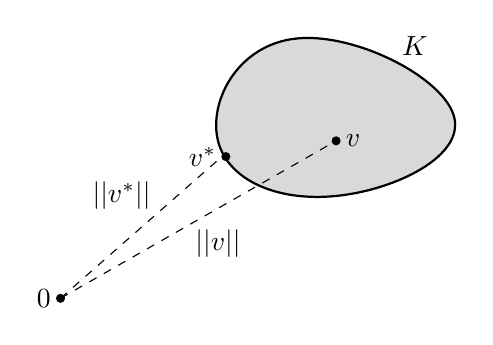
\begin{tikzpicture}
        \draw[style = thick, fill = gray!30!white] plot[smooth cycle, tension = 0.9, style = thick] coordinates{(1.5,1) (3,0.3) (4.5,1.3) (2.5,2.3)};
        \begin{scope}[style = dashed]
            \draw (-0.5,-1) -- (1.55,0.8);
            \draw (-0.5,-1) -- (3,1);
        \end{scope}
        \draw[fill = black] (-0.5,-1) circle[radius = 0.05] node[left] {$0$};
        \draw[fill = black] (1.6,0.8) circle[radius = 0.05] node[left] {$v^*$};
        \draw[fill = black] (3,1) circle[radius = 0.05] node[right] {$v$};
        \node at (0.275,0.3) {$||v^*||$};
        \node at (1.5,-0.3) {$||v||$};
        \node at (4,2.2) {$K$};
    \end{tikzpicture}
    \caption{정리 \ref{thm:smallestNorm}에서의 집합 $K$와 점 $v^*$.}
\end{figure}

\begin{proof}
    먼저 존재성을 보이기 위해 $\delta=\inf_{v\in K}||v||$라 하고 $||v_i||\to\delta$인 $K$에 속하는 수열 $\{v_i\}$를 생각하자. 이제 임의의 $\epsilon>0$을 택하면 적당한 $i_0\in\mathbb{N}$가 존재하여 임의의 $i\geq i_0$에 대해 $|||v_i||^2-\delta^2|<\epsilon/4$ 즉, $||v_i||^2<\delta^2+\epsilon/4$이다. 한편, 임의의 $i,\,j\geq i_0$에 대해 $K$가 볼록집합이므로 $(v_i+v_j)/2\in K$이고, 따라서 $||v_i+v_j||\geq2\delta$가 되어 이상으로부터 $||v_i-v_j||^2=2||v_i||^2+2||v_j||^2-||v_i+v_j||^2<4\delta^2+\epsilon-4\delta^2=\epsilon$이므로 $\{v_i\}$는 \texttt{Cauchy}이다. 그런데 가정으로부터 $\{v_i\}$는 $K$에서 수렴하고 그 수렴값을 $v^*\in K$라 하면 $||v_i||\to||v^*||=\delta$이므로 임의의 $v\in K$에 대해 $||v||\geq||v^*||$가 되어 존재성이 보여진다.

    유일성을 보이는 것은 보다 간단하다. 만약 $||v^*||=||\widetilde{v}||=\delta$인 $v^*$와 다른 $\widetilde{v}\in K$가 존재한다면 $K$가 볼록집합이므로 $(v^*+\widetilde{v})/2\in K$이고, 곧 $||v^*+\widetilde{v}||\geq2\delta$이다. 그런데 이는 $||v^*-\widetilde{v}||^2=2||v^*||^2+2||\widetilde{v}||^2-||v^*+\widetilde{v}||^2\leq4\delta^2-4\delta^2=0$에서 $v^*=\widetilde{v}$의 모순을 함의하므로 유일성이 보여진다.
\end{proof}

마침내, 짧았던 $L^p$ 공간과 추상세계에서의 여정에 마침표를 찍을 정리를 소개한다. \texttt{Riesz}의 표현정리라 불리는 다음 정리의 결론은 \texttt{Hilbert} 공간에서의 모든 유계인 선형사상은 그 공간의 벡터 하나로 완벽히 특정된다는 것이다. 즉, 선형사상이 유계이면 그 선형사상에 대한 정보는 점 하나에 모두 담겨있다!

\begin{theorem}[Riesz representation theorem]
    \texttt{Hilbert} 공간 $(\mathsf{V},\,||\cdot||)$에서 정의된 선형사상 $T:\mathsf{V}\to\mathbb{R}$가 유계라 하면 임의의 $v\in\mathsf{V}$에 대해 $T(v)=\langle v,\,v^*\rangle$인 $v^*\in\mathsf{V}$가 유일하게 존재한다. 나아가, 이러한 $v^*$에 대해 $||v^*||=||T||_{\mathrm{op}}$가 성립한다.
\end{theorem}

\begin{proof}
    먼저 존재성을 보이자. 만약 $T=0$이면 $v^*=0$이 정리의 조건을 만족하고 곧 정리가 자명하므로 $T\ne0$이라 하자. 이제 집합 $K=T^{-1}(1)$을 생각하면 가정으로부터 $T(v)\ne0$인 $v\in\mathsf{V}$를 적어도 하나 택할 수 있고, 이러한 $v$에 대해 $T(v/||T(v)||)=1$에서 $v/||T(v)||\in K$이므로 $K$는 공집합이 아니다. 또한, $T$가 유계이므로 이는 연속이고, 따라서 $K$는 닫혀있으며, 임의의 $v,\,w\in K$와 임의의 $t\in[0,\,1]$에 대해 $T(tv+(1-t)w)=tT(v)+(1-t)T(w)=1$이므로 $tv+(1-t)w\in K$가 되어 $K$는 볼록집합이다. 그렇다면 정리 \ref{thm:smallestNorm}로부터 임의의 $v\in K$에 대해 $||\widetilde{v}||\leq||v||$인 $\widetilde{v}\in K$가 유일하게 존재한다.

    존재성에 대한 증명을 마무리하기 위해서는 임의의 $v\in\ker T$에 대해 $\langle v,\,\widetilde{v}\rangle=0$임을 보이는 것으로 충분하다. 만약 이를 보일 수 있으면 임의의 $v\in\mathsf{V}$에 대해 $T(v-T(v)\widetilde{v})=T(v)-T(v)=0$에서 $v-T(v)\widetilde{v}\in\ker T$이므로 곧 $0=\langle v-T(v)\widetilde{v},\,\widetilde{v}\rangle=\langle v,\,\widetilde{v}\rangle-T(v)||\widetilde{v}||^2$에서 $v^*=\widetilde{v}/||\widetilde{v}||^2$라 하면 $T(v)=\langle v,\,\widetilde{v}\rangle/||\widetilde{v}||^2=\langle v,\,v^*\rangle$가 되어 존재성이 명백하기 때문이다. 이제 임의의 $v\in\ker T$를 택하면 임의의 $t\in\mathbb{R}$에 대해 $T(\widetilde{v}+tv)=T(\widetilde{v})+tT(v)=1$이므로 $\widetilde{v}+tv\in K$에서 $||\widetilde{v}||^2\leq||\widetilde{v}+tv||^2=||\widetilde{v}||^2+2t\langle v,\,\widetilde{v}\rangle+t^2||v||^2$이다. 이는 곧 함수 $t\mapsto||\widetilde{v}||^2+2t\langle v,\,\widetilde{v}\rangle+t^2||v||^2$가 $t=0$에서 최댓값을 가짐을 뜻하므로 그 도함수가 $0$을 근으로 가진다는 사실로부터 $\langle v,\,\widetilde{v}\rangle=0$이다.

    유일성을 보이는 것은 보다 간단하다. 만약 임의의 $v\in\mathsf{V}$에 대해 $T(v)=\langle v,\,v^*\rangle=\langle v,\,\widetilde{v}\rangle$인 $v^*$가 아닌 $\widetilde{v}\in\mathsf{V}$가 존재한다면 $\langle v,\,v^*-\widetilde{v}\rangle=0$인데, 여기서 $v=v^*-\widetilde{v}$를 택하면 $||v^*-\widetilde{v}||^2=\langle v^*-\widetilde{v},\,v^*-\widetilde{v}\rangle=0$이 되어 $v^*=\widetilde{v}$의 모순이 발생하므로 유일성이 보여진다.

    마지막으로, $||v^*||=||T||_{\mathrm{op}}$임을 보이자. 만약 $v^*=0$이면 명백히 $T=0$이므로 $||v^*||=||T||_\mathrm{op}=0$에서 정리가 자명하므로 $v^*\ne0$이라 하자. 그렇다면 $||v^*||=\langle v^*,\,v^*\rangle/||v^*||=T(v^*)/||v^*||\leq|T||_\mathrm{op}$이다. 한편, \texttt{Cauchy-Schwarz} 부등식으로부터 임의의 $v\in\mathsf{V}$에 대해 $|T(v)|=|\langle v,\,v^*\rangle|\leq||v||||v^*||$이므로 $||v^*||\geq|T(v)|/||v||$에서 $||T||_\mathrm{op}\leq||v^*||$이 되어 이상으로부터 $||v^*||=||T||_{\mathrm{op}}$임을 안다.
\end{proof}

\begin{corollary}
    측도공간 $(X,\,\mathcal{A},\,\mu)$와 선형사상 $T:L^2\to\mathbb{R}$에 대해 $T$가 유계라면 임의의 $g\in L^2$에 대해 $T(g)=\int_Xfg\,d\mu$인 $f\in L^2$가 존재하고, 거의 어디서나 같은 함수를 하나로 본다면 유일하다. 나아가 $||T||_{\mathrm{op}}=||f||_2$이다.
\end{corollary}

\begin{proof}
    정리 \ref{thm:lpHilbert}로부터 $(L^2,\,\langle\cdot,\,\cdot\rangle)$이 \texttt{Hilbert} 공간으므로 \texttt{Riesz}의 표현정리로부터 이는 거의 자명하다.
\end{proof}

이제 다시 측도공간으로 돌아오자. 다음의 정리나 개념들은 훨씬 전에 소개할 수도 있었지만 논의의 전개가 산만해지는 것을 피하기 위해 일부러 조금 미루어 두었던 것들이다. 먼저 $\sigma$-대수의 제한을 소개한다.

\begin{definition}
    가측공간 $(X,\,\mathcal{A})$와 공집합이 아닌 $Y\in\mathcal{A}$에 대해 집합족 $\{A\in\mathcal{A}:A\subseteq Y\}$를 $\mathcal{A}$의 $Y$로의 \textbf{제한(\texttt{restriction})}이라 하고 $\mathcal{A}\vert_Y$로 쓴다.
\end{definition}

\begin{proposition}\label{prop:restrictSigmaAlgebra}
    가측공간 $(X,\,\mathcal{A})$와 집합 $Y\in\mathcal{A}$에 대해 $\mathcal{A}\vert_Y$는 $Y$ 위의 $\sigma$-대수이다.
\end{proposition}

\begin{proof}
    우선 $Y\in\mathcal{A}\vert_Y$이므로 이는 비어있지 않고 임의의 $A\in\mathcal{A}\vert_Y$에 대해 $Y\setminus A\in\mathcal{A}\vert_Y$에서 $\mathcal{A}\vert_Y$는 ($Y$를 전체 공간으로 보았을 때의) 여집합에 대해서 닫혀있다. 한편, 이가 가산 합집합에 대해 닫혀있음은 분명하므로 이상으로부터 $\mathcal{A}\vert_Y$는 $Y$ 위의 $\sigma$-대수이다.
\end{proof}

\begin{theorem}\label{thm:intRistriction}
    측도공간 $(X,\,\mathcal{A},\,\mu)$와 집합 $Y\in\mathcal{A}$에 대해 $\mathcal{B}=\mathcal{A}\vert_Y$라 하면 다음이 성립한다.
    \begin{enumerate}
        \item 제한 $\mu\vert_\mathcal{B}$는 $\mathcal{B}$ 위의 측도이다. 따라서 $(X,\,\mathcal{B},\,\mu\vert_\mathcal{B})$는 측도공간을 이룬다.
        \item 가측공간 $(Z,\,\mathcal{C})$와 $\mathcal{A}/\mathcal{C}$-가측함수 $f:X\to Z$에 대해 $f\vert_Y$는 $\mathcal{B}/\mathcal{C}$-가측이다.
        \item 음이 아닌 $\mathcal{A}/\mathcal{B}_1$-가측함수 $f:X\to\overline{\mathbb{R}}^+_0$에 대해 $\int_Yf\,d\mu=\int_Yf\vert_Y\,d\mu\vert_{\mathcal{B}}$이다. 한편, $Y$에서 $\mu$-적분가능한(혹은 $f\vert_Y$가 $\mu\vert_\mathcal{B}$-적분가능한 $\mathcal{A}/\mathcal{B}_1$-가측함수) $f:X\to\overline{\mathbb{R}}$에 대해서도 동일한 결과가 성립하며, 이때 $f\vert_Y$는 $\mu\vert_\mathcal{B}$-적분가능하다(혹은 $f$는 $Y$에서 $\mu$-적분가능하다).
    \end{enumerate}
\end{theorem}

\begin{proof}
    i. 이는 명제 \ref{prop:restrictSigmaAlgebra}로부터 $\mathcal{B}$가 $Y$ 위의 $\sigma$-대수라는 점에서 자명하다.

    ii. 이 또한 거의 자명하다. 임의의 $A\in\mathcal{C}$에 대해 $(f\vert_Y)^{-1}(A)=f^{-1}(A)\cap Y\in\mathcal{B}$이므로 $f\vert_Y$가 $\mathcal{B}/\mathcal{C}$-가측이다.
    
    iii. 먼저 $f$가 음이 아닌 단순함수인 경우를 생각하여 이의 표준형을 $f=\sum_{i=1}^ka_i\ind_{A_i}$라 하면 $f\vert_Y=\sum_{i=1}^ka_i\ind_{A_i\cap Y}$이고, 이로부터 $\int_Yf\vert_Y\,d\mu\vert_\mathcal{B}=\sum_{i=1}^ka_i\mu\vert_\mathcal{B}(A_i\cap Y)=\sum_{i=1}^ka_i\mu(A_i\cap Y)=\int_Xf\ind_Y\,d\mu=\int_Yf\,d\mu$이다. 이제 $f$를 음이 아닌 가측함수라 하면 정리 \ref{thm:measurableFunctionApprox}로부터 음이 아닌 단순함수 $f_i:X\to\mathbb{R}^+_0$의 열 $\{f_i\}$가 존재하여 $f_i\uparrow f$이므로 \texttt{MCT}에서 $\int_Yf\vert_Y\,d\mu\vert_\mathcal{B}=\lim_{i\to\infty}\int_Yf_i\vert_Y\,d\mu\vert_\mathcal{B}=\lim_{i\to\infty}\int_Yf_i\,d\mu=\int_Yf\,d\mu$이다.

    한편, $Y$에서 $\mu$-적분가능한 $f:X\to\overline{\mathbb{R}}$에 대해서, 이를 양과 음의 부분으로 나누어 앞선 결과를 적용하면 $f\vert_Y$가 $\mu\vert_\mathcal{B}$-적분가능하며 $\int_Yf\vert_Y\,d\mu\vert_{\mathcal{B}}=\int_Yf\,d\mu$임을 쉽게 알 수 있고, $f\vert_Y$가 $\mu\vert_\mathcal{B}$-적분가능한 $\mathcal{A}/\mathcal{B}_1$-가측함수 $f:X\to\overline{\mathbb{R}}$에 대해서도 비슷하게 하면 된다.
\end{proof}

위의 정리는, 비록 그 표현은 복잡해 보이지만, 본질적으로는 피적분함수와 적분에 사용되는 측도의 적분영역 밖의 정보는 그 적분에 있어 아무런 필요가 없다는 지극히 상식적인 아이디어를 확인한 것에 불과하다.

다음으로, 측도의 선형결합에 대한 내용으로 넘어가자. 이 또한 매우 직관적인 결과들이다.

\begin{theorem}
    가측공간 $(X,\,\mathcal{A})$ 위의 측도 $\mu,\,\nu$에 대해 다음이 성립한다.
    \begin{enumerate}
        \item 임의의 $c\geq0$에 대해 함수 $c\mu$도 측도이다.
        \item 함수 $\mu+\nu$도 측도이다.
    \end{enumerate}
\end{theorem}

\begin{proof}
    자명하다. i의 $c\mu$와 ii의 $\mu+\nu$가 측도의 조건들을 만족함을 쉽게 확인할 수 있다.
\end{proof}

\begin{theorem}\label{thm:linearCombiMeasure}
    가측공간 $(X,\,\mathcal{A})$ 위의 측도 $\mu,\,\nu$와 음이 아닌 가측함수 $f:X\to\overline{\mathbb{R}}^+_0$에 대해 다음의 성립한다.
    \begin{enumerate}
        \item 임의의 $c\geq0$에 대해 $\int_Xf\,d(c\mu)=c\int_Xf\,d\mu$이다.
        \item $\int_Xf\,d(\mu+\nu)=\int_Xf\,d\mu+\int_Xf\,d\nu$이다.
    \end{enumerate}
    한편, $\mu$-적분가능한 $f:X\to\overline{\mathbb{R}}$에 대해서도 i의 성질이 성립하고, 이때 $f$는 $c\mu$-적분가능하다. 비슷하게, $\mu$-적분가능한 동시에 $\nu$-적분가능한(혹은 $(\mu+\nu)$-적분가능한) $f:X\to\overline{\mathbb{R}}$에 대해서도 ii의 성질이 성립하고, 이때 $f$는 $(\mu+\nu)$-적분가능하다(혹은 $\mu$-적분가능한 동시에 $\nu$-적분가능하다).
\end{theorem}

\begin{proof}
    편의를 위해 i만 증명하도록 한다. (ii는 i과 비슷하게 하면 된다.) 먼저 $f$가 음이 아닌 단순함수인 경우를 생각하여 이의 표준형을 $f=\sum_{i=1}^ka_i\ind_{A_i}$라 하면 $\int_Xf\,d(c\mu)=\sum_{i=1}^ka_i(c\mu)(A_i)=c\sum_{i=1}^ka_i\mu(A_i)=c\int_Xf\,d\mu$가 성립한다. 이제 $f$를 음이 아닌 가측함수라 하면 정리 \ref{thm:measurableFunctionApprox}로부터 음이 아닌 단순함수 $f_i:X\to\mathbb{R}^+_0$의 열 $\{f_i\}$가 존재하여 $f_i\uparrow f$이므로 \texttt{MCT}에서 $\int_Xf\,d(c\mu)=\lim_{i\to\infty}\int_Xf_i\,d(c\mu)=c\lim_{i\to\infty}\int_Xf_i\,d\mu=c\int_Xf\,d\mu$임을 안다. 

    한편, $\mu$-적분가능한 $f:X\to\overline{\mathbb{R}}$에 대해서, 이를 양과 음의 부분으로 나누어 앞선 결과를 적용하면 $f$가 $c\mu$-적분가능하며 $\int_Xf\,d(c\mu)=c\int_Xf\,d\mu$임을 쉽게 알 수 있다.
\end{proof}

이로써 도함수를 일반화하기 위한 준비가 모두 끝났다. 아마 아직은 감이 오지 않겠지만, 우리가 $L^p$ 공간과 \texttt{Hilbert} 공간을 오가며 얻은 결과들과 뜬금없이 소개한 $\sigma$-대수의 제한과 같은 내용들이 마법과 같이 하나로 합쳐져 우리가 원하는 도함수의 일반화로 이어질 것이다.

\begin{definition}
    가측공간 $(X,\,\mathcal{A})$ 위의 측도 $\mu,\,\nu$를 생각하자. 만약 $\nu(N)=0$인 모든 $N\in\mathcal{A}$에 대해 $\mu(N)=0$이면 이때 $\mu$는 $\nu$에 대해 \textbf{절대연속(\texttt{absolutely continuous})}이라 하고 $\mu\ll\nu$로 쓴다.
\end{definition}

\begin{lemma}
    유한 측도공간 $(X,\,\mathcal{A},\,\mu)$에 대해 $L^2\subseteq L^1$이다.
\end{lemma}

\begin{proof}
    임의의 $f\in L^2$에 대해 \texttt{Cauchy-Schwarz} 부등식으로부터 $\int_X|f|\,d\mu=\langle|f|,\,1\rangle\leq||f||_2||1||_2=\sqrt{(\int_Xf^2\,d\mu)(\int_X\,d\mu)}=\sqrt{\mu(X)}||f||_2<\infty$이고, 곧 $f\in L^1$이므로 $L^2\subseteq L^1$임을 안다.
\end{proof}

\begin{theorem}[Radon-Nikod\'ym]
    가측공간 $(X,\,\mathcal{A})$ 위의 측도 $\mu$와 $\sigma$-유한 측도 $\nu$에 대해 \texttt{TFAE}.
    \begin{enumerate}
        \item 측도 $\mu$는 $\sigma$-유한하고 $\mu\ll\nu$이다.
        \item 음이 아닌 가측함수 $f:X\to\mathbb{R}^+_0$가 존재하여 $\mu=\nu_f$이다.
    \end{enumerate}
    특히, 만약 i이 성립한다면 ii에서의 가측함수 $f$는 $\nu-$거의 어디서나 같은 함수를 하나로 본다면 유일하다. 나아가, 만약 $\mu$가 유한하다면 $f$는 $\nu$-적분가능하다.
\end{theorem}

\begin{proof}
    ii $\Rightarrow$ i. 우선 임의의 $N\in\mathcal{A}$에 대해 $\nu(N)=0$이라 하면 보조정리 \ref{cor:zeroAeIntegral}의 i로부터 $\mu(N)=\nu_f(N)=0$이 되어 $\mu\ll\nu$임은 분명하므로 $\mu$가 $\sigma$-유한함만 보이면 된다. 가정으로부터 $\nu$가 $\sigma$-유한하므로 $\mathcal{A}$에 속하는 적당한 $\{A_i\}$가 존재하여 각 $i\in\mathbb{N}$에 대해 $\nu(A_i)<\infty$이고 $\bigcup_{i=1}^\infty A_i=X$이며, \texttt{WLOG}, 필요하다면 각 항을 $C_i:=\bigcup_{j=1}^iA_j$로 바꾸어 $\{A_i\}$가 처음부터 증가하는 집합열이라 해도 된다. 이제 집합열 $\{B_i\}$를 $B_i=f^{-1}((-\infty,\,i])\cap A_i$라 하면 이는 명백히 증가하는 집합열로 각 $i\in\mathbb{N}$에 대해 $\mu(B_i)=\int_{B_i}f\,d\nu\leq\int_{A_i}i\,d\nu=i\nu(A_i)<\infty$이고 $\bigcup_{i=1}^\infty B_i=X$임이 분명하므로 $\mu$도 $\sigma$-유한하다.

    i $\Rightarrow$ ii. 우선 $\nu,\,\mu$가 모두 유한한 특별한 경우를 생각하자. 이제 함수 $T:L^2(\nu+\mu)\to\mathbb{R}$를 $T:g\mapsto\int_Xg\,d\mu$로 두면 $\nu,\,\mu$가 유한하므로 $\nu+\mu$도 유한하여 위의 보조정리와 정리 \ref{thm:linearCombiMeasure}의 ii로부터 $L^2(\nu+\mu)\subseteq L^1(\nu+\mu)\subseteq L^1(\mu)$이고, 곧 $T$는 \texttt{well-define}된다. 또한, $T$가 선형사상임이 분명하고 임의의 $g\in L^2(\nu+\mu)$에 대해 \texttt{Cauchy-Schwarz} 부등식으로부터
    \begin{align*}
        |T(g)|&=\bigg|\int_Xg\,d\mu\bigg|\\
        &\leq\int_X|g|\,d\mu\\
        &\leq\int_X|g|\,d\nu+\int_X|g|\,d\mu\\
        &=\int_X|g|\,d(\nu+\mu)\\
        &=\langle|g|,\,1\rangle_{\nu+\mu}\\
        &\leq||g||_{2,\,\nu+\mu}||1||_{2,\,\nu+\mu}\\
        &=\sqrt{\bigg[\int_Xg^2\,d(\nu+\mu)\bigg]\bigg[\int_X\,d(\nu+\mu)\bigg]}\\
        &=\sqrt{(\nu+\mu)(X)}||g||_{2,\,\nu+\mu}
    \end{align*}
    이므로 $T$는 유계인 선형사상이 되어 \texttt{Riesz}의 표현정리로부터 임의의 $g\in L^2(\nu+\mu)$에 대해 $\int_Xg\,d\mu=T(g)=\int_Xgh\,d(\nu+\mu)$인 $h\in L^2(\nu+\mu)$가 존재한다. 나아가 임의의 $g\in L^2(\nu+\mu)$에 대해 $\int_Xg(1-h)\,d(\nu+\mu)=\int_Xg\,d(\nu+\mu)-\int_Xgh\,d(\nu+\mu)=\int_Xg\,d(\nu+\mu)-\int_Xg\,d\mu=\int_Xg\,d\nu$도 성립한다.

    더 진행하기 전에 $0\leq h<1$ ($(\nu+\mu)$-\texttt{ae.})임을 확인하고 가자. 이를 위해 집합 $A=h^{-1}((-\infty,\,0)),\,B=h^{-1}([1,\,\infty))$를 생각하면 $\mu(A)=\int_X\ind_A\,d\mu=\int_Xh\ind_A\,d(\nu+\mu)\leq0$이므로 $\int_Xh\ind_A\,d(\nu+\mu)=0$이고 곧 정리 \ref{thm:zeroAeIntegral}의 ii로부터 $h\ind_A=0$ (($\nu+\mu$)-\texttt{ae.})가 되어 $(\nu+\mu)(A)=(\nu+\mu)((h\ind_A)^{-1}((-\infty,\,0)))=0$이다. 비슷하게, $\nu(B)=\int_X\ind_B\,d\nu=\int_X(1-h)\ind_B\,d(\nu+\mu)\leq0$이므로 $\nu(B)=0$이고, $\mu\ll\nu$라는 가정으로부터 $\mu(B)=0$이 되어 $(\nu+\mu)(B)=0$이다. 이상으로부터 $A,\,B$가 모두 $(\nu+\mu)$-영집합이 되어 $0\leq h<1$ ($(\nu+\mu)$-\texttt{ae.})이다.

    \texttt{WLOG}, 필요하다면 $(\nu+\mu)$-영집합에서의 $h$의 값을 $0$으로 바꾸어 그냥 $0\leq h<1$이라 해도 된다. 한편, 임의의 $A\in\mathcal{A}$에 대해 $\nu(A)=\int_X\ind_A\,d\nu=\int_X(1-h)\ind_A\,d(\nu+\mu)=\int_A1-h\,d(\nu+\mu)=(\nu+\mu)_{1-h}(A)$이므로 임의의 음이 아닌 가측함수 $g:X\to\overline{\mathbb{R}}^+_0$에 대해 $\int_Xg\,d\nu=\int_Xg\,d(\nu+\mu)_{1-h}=\int_Xg(1-h)\,d(\nu+\mu)$이다. 따라서 함수 $f:X\to\overline{\mathbb{R}}^+_0$를 $f=h/(1-h)$로 두면 이는 가측이고 임의의 $A\in\mathcal{A}$에 대해 $\mu(A)=\int_X\ind_A\,d\mu=\int_Xh\ind_A\,d(\nu+\mu)=\int_Xf(1-h)\ind_A\,d(\nu+\mu)=\int_Xf\ind_A\,d\nu=\int_Af\,d\nu$가 되어 $\mu=\nu_f$에서 정리가 성립한다.

    이제 $\sigma$-유한한 $\nu,\,\mu$를 생각하면 정의로부터 $\mathcal{A}$에 속하는 적당한 $\{A_i\},\,\{B_i\}$가 존재하여 $\bigcup_{i=1}^\infty A_i=\bigcup_{i=1}^\infty B_i=X$이고 각 $i\in\mathbb{N}$에 대해 $\nu(A_i),\,\mu(B_i)<\infty$이다. 또한, 앞서 ii가 i을 함의함을 증명할 때와 비슷하게 하여 \texttt{WLOG}, $\{A_i\},\,\{B_i\}$가 증가한다고 해도 된다. 이제 집합열 $\{Y_i\}$를 $Y_i=A_i\cap B_i$로 두면 이는 증가하는 집합열로서 $\bigcup_{i=1}^\infty Y_i=\bigcup_{i=1}^\infty A_i\cap\bigcup_{i=1}^\infty B_i=X$이고 각 $i\in\mathbb{N}$에 대해 $\nu(Y_i)\leq\nu(A_i)<\infty$이며 $\mu(Y_i)\leq\mu(B_i)<\infty$이다. 또한, 표기의 편의를 위해 각 $i\in\mathbb{N}$에 대해 $\mathcal{B}_i=\mathcal{A}\vert_{Y_i},\,\nu_i=\nu\vert_{\mathcal{B}_i},\,\mu_i=\mu\vert_{\mathcal{B}_i}$로 두면 $\nu_i,\,\mu_i$는 유한하며 $\mathcal{B}_{i+1}\vert_{Y_i}=\mathcal{B}_i,\,\nu_{i+1}\vert_{\mathcal{B}_i}=\nu_i,\,\mu_{i+1}\vert_{\mathcal{B}_i}=\mu_i$이다. 그렇다면 각 $i\in\mathbb{N}$에 대해 $\mu_i\ll\nu_i$임이 분명하므로 앞선 결과로부터 적당한 음이 아닌 가측함수 $f_i:Y_i\to\mathbb{R}^+_0$가 존재하여 $\mu_i=(\nu_i)_{f_i}$이고, 각 $i\in\mathbb{N}$와 임의의 $A\in\mathcal{B}_i$에 대해 정리 \ref{thm:intRistriction}로부터 $\int_Af_i\,d\nu_i=(\nu_i)_{f_i}(A)=\mu_i(A)=\mu_{i+1}(A)=(\nu_{i+1})_{f_{i+1}}(A)=\int_Af_{i+1}\,d\nu_{i+1}=\int_Af_{i+1}\vert_{Y_i}\,d\nu_i$이다. 이는 곧 정리 \ref{thm:twoFuncIntEqual}로부터 각 $i\in\mathbb{N}$에 대해 $f_i=f_{i+1}\vert_{Y_i}$ ($\nu_i$-\texttt{ae.})임을 함의하므로 \texttt{WLOG}, 필요하다면 $\nu_i$-영집합에서의 $f_{i+1}$의 값을 조금씩 바꾸어 그냥 $f_i=f_{i+1}\vert_{Y_i}$라 해도 되고, 이로부터 함수 $f:X\to\mathbb{R}^+_0$를 임의의 $i\in\mathbb{N}$에 대해 $f\vert_{Y_i}=f_i$가 되도록 정의할 수 있다. 그렇다면 임의의 $x\in\mathbb{R}$에 대해 $f^{-1}((-\infty,\,x])=\bigcup_{i=1}^\infty[f^{-1}((-\infty,\,x])\cap Y_i]=\bigcup_{i=1}^\infty(f_i)^{-1}((-\infty,\,x])$이므로 $f$는 가측이다. 이제 임의의 $C\in\mathcal{A}$에 대해 집합열 $\{C_i\}$를 $C_i=C\cap Y_i$로 두면 $C_i\uparrow C$이므로 정리 \ref{thm:monoSeriesMeasure}의 i과 정리 \ref{thm:monoSeriesIntegral}의 i로부터
    \begin{align*}
        \mu(C)&=\lim_{i\to\infty}\mu(C_i)\\
        &=\lim_{i\to\infty}\mu_i(C_i)\\
        &=\lim_{i\to\infty}(\nu_i)_{f_i}(C_i)\\
        &=\lim_{i\to\infty}\int_{C_i}f_i\,d\nu_i\\
        &=\lim_{i\to\infty}\int_{C_i}f\,d\nu\\
        &=\int_Cf\,d\nu\\
        &=\nu_f(C)
    \end{align*}
    가 되어 $\mu=\nu_f$이다.

    한편, 정리 \ref{thm:twoFuncIntEqual}로부터 이러한 $f$가 $\nu-$거의 어디서나 같은 함수를 하나로 본다면 유일함이 분명하고, 만약 $\mu$가 유한하다면 $\int_Xf\,d\nu=\nu_f(X)=\mu(X)<\infty$에서 $f$가 $\nu$-적분가능하므로 증명이 끝난다.
\end{proof}

\begin{definition}\label{def:radonNikodym}
    가측공간 $(X,\,\mathcal{A})$ 위의 $\sigma$-유한 측도 $\mu,\,\nu$에 대해 $\mu\ll\nu$이면 이때 $\mu=\nu_f$를 만족하는 함수 $f:X\to\mathbb{R}^+_0$를 $\mu$의 $\nu$에 대한 \textbf{\texttt{Radon-Nikod\'ym} 도함수(- \texttt{derivative})}라 하고 $d\mu/d\nu$로 쓴다.
\end{definition}

치환적분법을 떠오르게 하는 다음 따름정리를 보면 방금 우리가 얻은 정의를 왜 도함수의 일반화로 볼 수 있는지가 더욱 분명해 질 것이다.

\begin{corollary}\label{cor:radonNikodym}
    가측공간 $(X,\,\mathcal{A})$ 위의 $\sigma$-유한 측도 $\nu,\,\mu$에 대해 $\mu\ll\nu$라 하자. 그렇다면 임의의 음이 아닌 가측함수 $f:X\to\overline{\mathbb{R}}^+_0$에 대해 $\int_Xf\,d\mu=\int_Xf(d\mu/d\nu)\,d\nu$이다. 한편, $\mu$-적분가능한(혹은 $f(d\mu/d\nu)$가 $\nu$-적분가능한 가측함수) $f:X\to\overline{\mathbb{R}}$에 대해서도 동일한 결과가 성립하며 이때 $f(d\mu/d\nu)$는 $\nu$-적분가능하다(혹은 $f$는 $\mu$-적분가능하다).
\end{corollary}

\begin{proof}
    이는 정리 \ref{thm:intInducedMeasure}로부터 자명하다.
\end{proof}

\section{\texttt{Fubini}'s Theorem}

이번 절에서는 그 제목에서와 같이 다중적분을 반복적분으로써 계산할 수 있도록 해 주는 \texttt{Fubini}의 정리를 증명한다. 사실 이전 절에서 보인 바와 같이 \texttt{Lebesgue} 적분은 \texttt{Riemann} 적분을 포괄하는 개념이므로 실제로 그 적분값을 구해야 할 필요가 있을 때에는 이를 \texttt{Riemann} 적분으로 생각하여 계산하면 되고, 미적분학이나 해석학에서 \texttt{Riemann} 적분에서의 \texttt{Fubini}의 정리를 이미 배웠으므로 이번 절에서의 논의가 없더라도 계산에 있어 \texttt{Fubini}의 정리를 사용할 수 있다. 그럼에도 불구하고, 하나의 절을 할애하여 이에 관한 논의를 진행하는 것에는 나름의 이유가 있다.

먼저, 종전에 우리가 배운 \texttt{Riemann} 적분에서의 \texttt{Fubini}의 정리는 피적분함수에 대해, 예컨대 이가 미분가능해야 한다거나, 혹은 조각적 연속이어야 한다거나 하는 다소 강한 조건을 요구한다. 또한, 어디까지나 \texttt{Lebesgue} 적분이 \texttt{Riemann} 적분을 포괄하는 것이지 이 두 개념이 서로 동등한 것이 아니므로 \texttt{Lebesgue} 적분을 언제나 \texttt{Riemann} 적분으로 생각하여 계산할 수 있는 것은 아니다. 예컨대 \texttt{Riemann} 적분은 불가능하지만 \texttt{Lebesgue} 적분은 가능한 대표적인 함수인 $\ind_{\mathbb{Q}\cap[0,\,1]}$의 적분을 계산해야 하는 경우, 이는 \texttt{Lebesgue} 적분으로만 계산할 수 있다.\footnotemark 비록 이러한 경우가 이 책에서는 (아마) 없겠지만, 그래도 이론적인 측면에서 조금 불안한 것이 사실이다. 이에 이번 절에서 \texttt{Fubini}의 정리를 \texttt{Lebesgue} 적분론의 틀 안에서 최대한 일반적으로 다시 증명함으로써 이런 이론적인 불안정함을 해소하고자 한다.

우선 가장 기본적인 형태로 \texttt{product measure space}에서 정의된 음이 아닌 가측함수에 대한 \texttt{Fubini}의 정리를 보자.

\begin{lemma}\label{lem:fubini1}
    $\sigma$-유한 측도공간 $(X,\,\mathcal{A},\,\mu),\,(Y,\,\mathcal{B},\,\nu)$와 음이 아닌 $(\mathcal{A}\otimes\mathcal{B})/\mathcal{B}_1$-가측함수 $f:X\times Y\to\overline{\mathbb{R}}^+_0$에 대해 함수 $\varphi:X\to\overline{\mathbb{R}}^+_0,\,\psi:Y\to\overline{\mathbb{R}}^+_0$를 각각 $\varphi:x\mapsto\int_Yf_x\,d\nu,\,\psi:y\mapsto\int_Xf^y\,d\mu$라 하면 이는 \texttt{well-define}되며 각각 $\mathcal{A}/\mathcal{B}_1$-가측이고 $\mathcal{B}/\mathcal{B}_1$-가측이다.
\end{lemma}

\begin{proof}
    우선 정리 \ref{thm:sectionMeasurable}로부터 모든 $x\in X$에 대해 $f_x$가 $\mathcal{B}/\mathcal{B}_1$-가측이므로 함수 $\varphi$는 \texttt{well-define}된다. 이제 $f$가 음이 아닌 단순함수인 특별한 경우를 생각하여 이의 표준형을 $f=\sum_{i=1}^ka_i\ind_{A_i}$라 하자. 그렇다면 $\varphi(x)=\int_Y(\sum_{i=1}^ka_i\ind_{A_i})_x\,d\nu=\sum_{i=1}^ka_i\int_Y\ind_{(A_i)_x}\,d\nu=\sum_{i=1}^ka_i\nu((A_i)_x)$이므로 보조정리 \ref{lem:productMeasure}로부터 $\varphi$가 $\mathcal{A}/\mathcal{B}_1$-가측이다. 한편, 음이 아닌 가측함수 $f$의 경우에는 정리 \ref{thm:measurableFunctionApprox}로부터 음이 아닌 단순함수 $f_i:X\times Y\to\mathbb{R}^+_0$의 열 $\{f_i\}$가 존재하여 $f_i\uparrow f$이고, 각 $i\in\mathbb{N}$에 대해 함수 $\varphi_i:X\to\overline{\mathbb{R}}^+_0$를 $\varphi_i:x\mapsto\int_Y(f_i)_x\,d\nu$라 하면 앞선 결과로부터 이는 $\mathcal{A}/\mathcal{B}_1$-가측이다. 그렇다면 \texttt{MCT}로부터 $\lim_{i\to\infty}\varphi_i(x)=\int_Y\lim_{i\to\infty}(f_i)_x\,d\nu=\int_Yf_x\,d\nu=\varphi(x)$이므로 정리 \ref{thm:limitMeasurable}의 ii로부터 $\varphi$는 $\mathcal{A}/\mathcal{B}_1$-가측이다. 이제 $\psi$에 대해서도 이와 비슷하게 하면 된다.
\end{proof}

\begin{theorem}[Fubini]
    $\sigma$-유한 측도공간 $(X,\,\mathcal{A},\,\mu),\,(Y,\,\mathcal{B},\,\nu)$와 $(\mathcal{A}\otimes\mathcal{B})/\mathcal{B}_1$-가측함수 $f:X\times Y\to\overline{\mathbb{R}}^+_0$에 대해
    \begin{equation*}
        \int_{X\times Y}f(x,\,y)\,d(\mu\otimes\nu)(x,\,y)=\int_X\bigg[\int_Yf(x,\,y)\,d\nu(y)\bigg]\,d\mu(x)=\int_Y\bigg[\int_Xf(x,\,y)\,d\mu(x)\bigg]\,d\nu(y)
    \end{equation*}
    가 성립한다.
\end{theorem}

\begin{proof}
    먼저 위의 보조정리로부터 이중적분들이 \texttt{well-define}됨을 안다. 이제 함수 $\varphi:X\to\overline{\mathbb{R}}^+_0$를 위의 보조정리에서와 같이 두고 $f$가 음이 아닌 단순함수인 특별한 경우를 생각하여 이의 표준형을 $f=\sum_{i=1}^ka_i\ind_{A_i}$라 하면 위의 보조정리의 증명에서 $\varphi(x)=\sum_{i=1}^ka_i\nu((A_i)_x)$이므로 정리 \ref{thm:productMeasure}로부터 $\int_X\varphi\,d\mu=\sum_{i=1}^ka_i\int_X\nu((A_i)_x)\,d\mu(x)=\sum_{i=1}^ka_i(\mu\otimes\nu)(A_i)=\int_{X\times Y}f\,d(\mu\otimes\nu)$이다. 한편, 음이 아닌 가측함수 $f$의 경우에는 정리 \ref{thm:measurableFunctionApprox}로부터 음이 아닌 단순함수 $f_i:X\times Y\to\mathbb{R}^+_0$의 열 $\{f_i\}$가 존재하여 $f_i\uparrow f$이고 함수열 $\{\varphi_i\}$를 위의 보조정리의 증명에서와 같이 두면 $\varphi_i\uparrow\varphi$이므로 \texttt{MCT}와 앞선 결론으로부터 $\int_X\varphi\,d\mu=\lim_{i\to\infty}\int_X\varphi_i\,d\mu=\lim_{i\to\infty}\int_{X\times Y}f_i\,d(\mu\otimes\nu)=\int_{X\times Y}f\,d(\mu\otimes\nu)$이다. 이제, 두 번째 등식에 대해서도 이와 비슷하게 하면 된다.
\end{proof}

다음으로, \texttt{product measure space}에서 정의된 적분가능한 함수에 대한 \texttt{Fubini}의 정리를 볼텐데, 이 경우에는 피적분함수의 \texttt{section}이 항상 적분가능하지 않으므로 조금 더 복잡하다.

\begin{lemma}\label{lem:fubini2}
    $\sigma$-유한 측도공간 $(X,\,\mathcal{A},\,\mu),\,(Y,\,\mathcal{B},\,\nu)$와 $(\mu\otimes\nu)$-적분가능한 함수 $f:X\times Y\to\overline{\mathbb{R}}$에 대해 다음이 성립한다.
    \begin{enumerate}
        \item \texttt{Section} $f_x:Y\to\overline{\mathbb{R}}$는 $\mu$-거의 대부분의 $x\in X$에 대해 $\nu$-적분가능하며 함수 $\varphi:X\to\mathbb{R}$를
        \begin{equation*}
            \varphi:x\mapsto
            \begin{dcases*}
                \int_Yf_x\,d\nu&$f_x$가 $\nu$-적분가능한 경우\\
                0&\texttt{ow.}
            \end{dcases*}
        \end{equation*}
        라 하면 이는 $\mu$-적분가능하다.
        \item \texttt{Section} $f^y:X\to\overline{\mathbb{R}}$는 $\nu$-거의 대부분의 $y\in Y$에 대해 $\mu$-적분가능하며 함수 $\psi:Y\to\mathbb{R}$를
        \begin{equation*}
            \psi:x\mapsto
            \begin{dcases*}
                \int_Xf^y\,d\mu&$f^y$가 $\mu$-적분가능한 경우\\
                0&\texttt{ow.}
            \end{dcases*}
        \end{equation*}
    라 하면 이는 $\nu$-적분가능하다.
    \end{enumerate}
\end{lemma}

\begin{proof}
    간결한 논의를 위해 i만 보이도록 하자. (ii는 i과 비슷하게 하면 된다.) 함수 $f_\pm$가 $(\mathcal{A}\otimes\mathcal{B})/\mathcal{B}_1$-가측이므로 함수 $\widetilde{\varphi}^\pm:X\to\overline{\mathbb{R}}^+_0$를 $\widetilde{\varphi}^\pm:x\mapsto\int_Y(f_\pm)_x\,d\nu$로 두면 (여기서 위첨자로 쓰인 $\pm$은 정의 \ref{def:integral}에서 아래첨자로 사용된 $\pm$와는 달리 함수의 양과 음의 부분을 의미하는 것이 아니다.) 이는 보조정리 \ref{lem:fubini1}로부터 $\mathcal{A}/\mathcal{B}_1$-가측이고, 곧 \texttt{Fubini}의 정리로부터 $\int_X\widetilde{\varphi}^\pm\,d\mu=\int_{X\times Y}f_\pm\,d(\mu\otimes\nu)\leq\int_{X\times Y}|f|\,d(\mu\otimes\nu)<\infty$가 되어 $\widetilde{\varphi}^\pm$이 $\mu$-적분가능함을 안다. 그렇다면 $\widetilde{\varphi}^\pm$이 $\mu$-거의 어디서나 유한하므로 명백히 $\mathcal{A}$-가측인 집합 $N=(\widetilde{\varphi}^\pm)^{-1}(\infty)=\{x\in X:\int_Y|f_x|\,d\nu=\infty\}$에 대해 $\mu(N)=0$이고, 곧 $f_x$는 $\mu$-거의 대부분의 $x\in X$에 대해 $\nu$-적분가능하다. 이제 함수 $\varphi^\pm:X\to\mathbb{R}^+_0$를 $\varphi^\pm=\widetilde{\varphi}^\pm\ind_{X\setminus N}$로 두면 $\varphi^\pm=\widetilde{\varphi}^\pm$ ($\mu$-\texttt{ae.})이므로 따름정리 \ref{cor:zeroAeIntegral}의 ii로부터 $\varphi^\pm$은 $\mu$-적분가능하고, 임의의 $x\in X$에 대해 $(f_x)_\pm=(f_\pm)_x$가 성립하여 $\varphi=\varphi^+-\varphi^-$이므로 증명이 끝난다.
\end{proof}

\begin{theorem}[Fubini]
    $\sigma$-유한 측도공간 $(X,\,\mathcal{A},\,\mu),\,(Y,\,\mathcal{B},\,\nu)$와 $(\mu\otimes\nu)$-적분가능한 함수 $f:X\times Y\to\overline{\mathbb{R}}$에 대해
    \begin{equation*}
        \int_{X\times Y}f(x,\,y)\,d(\mu\otimes\nu)(x,\,y)=\int_X\bigg[\int_Yf(x,\,y)\,d\nu(y)\bigg]\,d\mu(x)=\int_Y\bigg[\int_Xf(x,\,y)\,d\mu(x)\bigg]\,d\nu(y)
    \end{equation*}
    가 성립한다. 단, 만약 고정된 $x\in X$에 대해 $f(x,\,y)$가 $\nu$-적분가능하지 않다면 이때의 $\int_Yf(x,\,y)\,d\nu(y)$의 값은 0으로 간주하고, 이는 고정된 $y\in Y$에 대해 $f(x,\,y)$가 $\mu$-적분가능하지 않은 경우에도 마찬가지이다.
\end{theorem}

\begin{proof}
    먼저 위의 보조정리로부터 이중적분들이 \texttt{well-define}됨을 안다. 이제 함수 $\varphi:X\to\mathbb{R}$와 $\varphi^\pm:X\to\mathbb{R}^+_0$를 각각 위의 보조정리와 그 증명에서와 같이 두면 $\varphi=\varphi^+-\varphi^-$에서 $\int_X\varphi\,d\mu=\int_X\varphi^+\,d\mu-\int_X\varphi^-\,d\mu=\int_{X\times Y}f_+\,d(\mu\otimes\nu)-\int_{X\times Y}f_-\,d(\mu\otimes\nu)=\int_{X\times Y}f\,d(\mu\otimes\nu)$임을 쉽게 알 수 있다. 이제 두 번째 등식에 대해서도 이와 비슷하게 하면 된다.
\end{proof}

비록 위의 정리에서는 적분불가능한 \texttt{section}에 대해 그 적분값을 0이라는 \texttt{dummy value}로 두었지만, 보조정리 \ref{lem:fubini2}로부터 피적분함수의 거의 대부분의 \texttt{section}이 적분가능하므로 전체 적분의 값은 \texttt{dummy value}의 선택과는 무관하다. 그리고 이로부터 위의 반복적분 표기는 나름 \texttt{make sense}한다. 이러한 사실은 뒤따르는 나머지 \texttt{Fubini}의 정리에 대해서도 마찬가지이다.

이제 중간 결과로서 \texttt{Borel} 측도공간에서의 \texttt{Fubini}의 정리를 얻는다.

\begin{corollary}
    $l+m=n$인 $l,\,m,\,n\in\mathbb{N}$과 음이 아닌 \texttt{Borel} 함수 $f:\mathbb{R}^n\to\overline{\mathbb{R}}^+_0$에 대해
    \begin{equation*}
        \int_{\mathbb{R}^n}f(x,\,y)\,d\mu_n(x,\,y)=\int_{\mathbb{R}^l}\bigg[\int_{\mathbb{R}^m}f(x,\,y)\,d\mu_m(y)\bigg]\,d\mu_l(x)=\int_{\mathbb{R}^m}\bigg[\int_{\mathbb{R}^l}f(x,\,y)\,d\mu_l(x)\bigg]\,d\mu_m(y)
    \end{equation*}
    가 성립한다. 한편, 적분가능한 \texttt{Borel} 함수 $f:\mathbb{R}^n\to\overline{\mathbb{R}}$에 대해서도 동일한 결과가 성립한다. 단, 이 경우에는 만약 고정된 $x\in\mathbb{R}^l$에 대해 $f(x,\,y)$가 적분가능하지 않다면 이때의 $\int_{\mathbb{R}^m}f(x,\,y)\,d\mu_m(y)$의 값은 0으로 간주하고, 이는 고정된 $y\in\mathbb{R}^m$에 대해 $f(x,\,y)$가 적분가능하지 않은 경우에도 마찬가지이다.
\end{corollary}

\begin{proof}
    이는 \texttt{Fubini}의 정리와 정리 \ref{thm:productLebesgue}의 i로부터 자명하다.
\end{proof}

한편, \texttt{Lebesgue} 측도공간은 \texttt{Borel} 측도공간과는 달리 \texttt{product measure space}의 완비화로써 구성되므로 조금 더 복잡한 \texttt{Fubini}의 정리가 필요하다. 논의의 전체적인 전개 방향은 이전과 비슷하다.

\begin{lemma}\label{lem:fubini3}
    $\sigma$-유한 완비측도공간 $(X,\,\mathcal{A},\,\mu),\,(Y,\,\mathcal{B},\,\nu)$와 음이 아닌 $\overline{\mathcal{A}\otimes\mathcal{B}}/\mathcal{B}_1$-가측함수 $f:X\times Y\to\overline{\mathbb{R}}^+_0$에 대해 다음이 성립한다.
    \begin{enumerate}
        \item \texttt{Section} $f_x:Y\to\overline{\mathbb{R}}$는 $\mu$-거의 대부분의 $x\in X$에 대해 $\mathcal{B}/\mathcal{B}_1$-가측이며 함수 $\varphi:X\to\overline{\mathbb{R}}^+_0$를
        \begin{equation*}
            \varphi:x\mapsto
            \begin{dcases*}
                \int_Yf_x\,d\nu&$f_x$가 $\mathcal{B}/\mathcal{B}_1$-가측인 경우\\
                0&\texttt{ow.}
            \end{dcases*}
        \end{equation*}
        라 하면 이는 $\mathcal{A}/\mathcal{B}_1$-가측이다.
        \item \texttt{Section} $f^y:X\to\overline{\mathbb{R}}$는 $\nu$-거의 대부분의 $y\in Y$에 대해 $\mathcal{A}/\mathcal{B}_1$-가측이며 함수 $\psi:Y\to\overline{\mathbb{R}}^+_0$를
        \begin{equation*}
            \psi:x\mapsto
            \begin{dcases*}
                \int_Xf^y\,d\mu&$f^y$가 $\mathcal{A}/\mathcal{B}_1$-가측인 경우\\
                0&\texttt{ow.}
            \end{dcases*}
        \end{equation*}
    라 하면 이는 $\mathcal{B}/\mathcal{B}_1$-가측이다.
    \end{enumerate}
\end{lemma}

\begin{proof}
    간결한 논의를 위해 i만 보이도록 하자. (ii는 i과 비슷하게 하면 된다.) 정리 \ref{thm:measureCompletionApprox}로부터 적당한 $(\mathcal{A}\otimes\mathcal{B})/\mathcal{B}_1$-가측함수 $g:X\times Y\to\overline{\mathbb{R}}$가 존재하여 $f=g$ ($(\mu\otimes\nu)$-\texttt{ae.})이고, \texttt{WLOG}, 필요하다면 $(\mu\otimes\nu)$-영집합에서의 $g$의 값을 0으로 바꾸어 $g$를 음이 아니라 해도 된다. 그렇다면 집합 $M=\{(x,\,y)\in X\times Y:f(x,\,y)\ne g(x,\,y)\}$에 대해 $(\mu\otimes\nu)(M)=0$이므로 정리 \ref{thm:productMeasure}로부터 $\int_x\nu(M_x)\,d\mu(x)=(\mu\otimes\nu)(M)=0$이고, 정리 \ref{thm:zeroAeIntegral}로부터 명백히 $\mathcal{A}$-가측인 집합 $N=\{x\in X:\nu(M_x)\ne0\}$에 대해 $\mu(N)=0$이다. 이상을 종합하면 임의의 $x\in X\setminus N$에 대해 $[(X\times Y)\setminus M]_x=Y\setminus M_x$ 위에서 $f_x=g_x$이므로 곧 $\mu$-거의 대부분의 $x\in X$에 대해 $f_x=g_x$ ($\nu$-\texttt{ae.})이고, 정리 \ref{thm:equalityAeMeasurable}와 보조정리 \ref{lem:fubini1}로부터 $f_x$는 $\mu$-거의 대부분의 $x\in X$에 대해 $\mathcal{B}/\mathcal{B}_1$-가측이다. 나아가, 함수 $\widetilde{\varphi}:X\to\overline{\mathbb{R}}^+_0$를 $\widetilde{\varphi}:x\mapsto\int_Yg_x\,d\nu$로 두면 다시 보조정리 \ref{lem:fubini1}로부터 이는 $\mathcal{A}/\mathcal{B}_1$-가측이 되고, 따름정리 \ref{cor:zeroAeIntegral}의 ii에서 $\varphi=\widetilde{\varphi}$ ($\mu$-\texttt{ae.})이므로 정리 \ref{thm:equalityAeMeasurable}로부터 $\varphi$는 $\mathcal{A}/\mathcal{B}_1$-가측이다.
\end{proof}

\begin{theorem}[Fubini]
    $\sigma$-유한 완비측도공간 $(X,\,\mathcal{A},\,\mu),\,(Y,\,\mathcal{B},\,\nu)$와 음이 아닌 $\overline{\mathcal{A}\otimes\mathcal{B}}/\mathcal{B}_1$-가측함수 $f:X\times Y\to\overline{\mathbb{R}}^+_0$에 대해
    \begin{equation*}
        \int_{X\times Y}f(x,\,y)\,d\overline{\mu\otimes\nu}(x,\,y)=\int_X\bigg[\int_Yf(x,\,y)\,d\nu(y)\bigg]\,d\mu(x)=\int_Y\bigg[\int_Xf(x,\,y)\,d\mu(x)\bigg]\,d\nu(y)
    \end{equation*}
    가 성립한다. 단, 만약 고정된 $x\in X$에 대해 $f(x,\,y)$가 $\mathcal{B}/\mathcal{B}_1$-가측이 아니라면 이때의 $\int_Yf(x,\,y)\,d\nu(y)$의 값은 0으로 간주하고, 이는 고정된 $y\in Y$에 대해 $f(x,\,y)$가 $\mathcal{A}/\mathcal{B}_1$-가측이 아닌 경우에도 마찬가지이다.
\end{theorem}
f
\begin{proof}
    먼저 위의 보조정리로부터 이중적분들이 \texttt{well-define}됨을 안다. 이제 함수 $\widetilde{\varphi}:X\to\overline{\mathbb{R}}^+_0$와 $g:X\times Y\to\overline{\mathbb{R}}^+_0$를 위의 보조정리의 증명에서와 같이 두면 $\varphi=\widetilde{\varphi}$ ($\mu$-\texttt{ae.})에서 \texttt{Fubini}의 정리와 따름정리 \ref{cor:zeroAeIntegral}의 ii, 정리 \ref{thm:measureCompletionInt}로부터 $\int_X\varphi\,d\mu=\int_X\widetilde{\varphi}\,d\mu=\int_{X\times Y}g\,d(\mu\otimes\nu)=\int_{X\times Y}g\,d\overline{\mu\otimes\nu}=\int_{X\times Y}f\,d\overline{\mu\otimes\nu}$이다. 이제 두 번째 등식에 대해서도 이와 비슷하게 하면 된다.
\end{proof}

\begin{lemma}
    $\sigma$-유한 완비측도공간 $(X,\,\mathcal{A},\,\mu),\,(Y,\,\mathcal{B},\,\nu)$와 $\overline{\mu\otimes\nu}$-적분가능한 함수 $f:X\times Y\to\overline{\mathbb{R}}$에 대해 다음이 성립한다.
    \begin{enumerate}
        \item \texttt{Section} $f_x:Y\to\overline{\mathbb{R}}$는 $\mu$-거의 대부분의 $x\in X$에 대해 $\nu$-적분가능하며 함수 $\varphi:X\to\mathbb{R}$를
        \begin{equation*}
            \varphi:x\mapsto
            \begin{dcases*}
                \int_Yf_x\,d\nu&$f_x$가 $\nu$-적분가능한 경우\\
                0&\texttt{ow.}
            \end{dcases*}
        \end{equation*}
        라 하면 이는 $\mu$-적분가능하다.
        \item \texttt{Section} $f^y:X\to\overline{\mathbb{R}}$는 $\nu$-거의 대부분의 $y\in Y$에 대해 $\mu$-적분가능하며 함수 $\psi:Y\to\mathbb{R}$를
        \begin{equation*}
            \psi:x\mapsto
            \begin{dcases*}
                \int_Xf^y\,d\mu&$f^y$가 $\mu$-적분가능한 경우\\
                0&\texttt{ow.}
            \end{dcases*}
        \end{equation*}
    라 하면 이는 $\nu$-적분가능하다.
    \end{enumerate}
\end{lemma}

\begin{proof}
    증명은 보조정리 \ref{lem:fubini2}와 거의 비슷하다. 이번에도 간결한 논의를 위해 i만 보이도록 하자. (ii는 i과 비슷하게 하면 된다.) 함수 $f_\pm$가 $\overline{\mathcal{A}\otimes\mathcal{B}}/\mathcal{B}_1$-가측이므로 함수 $\widetilde{\varphi}^\pm:X\to\overline{\mathbb{R}}^+_0$를
    \begin{equation*}
        \widetilde{\varphi}^\pm:x\mapsto
        \begin{dcases*}
            \int_Y(f_\pm)_x\,d\nu&$(f_\pm)_x$가 $\mathcal{B}/\mathcal{B}_1$-가측인 경우\\
            0&\texttt{ow.}
        \end{dcases*}
    \end{equation*}
    로 두면(여기서 위첨자로 쓰인 $\pm$은 정의 \ref{def:integral}에서 아래첨자로 사용된 $\pm$와는 달리 함수의 양과 음의 부분을 의미하는 것이 아니다.) 보조정리 \ref{lem:fubini3}로부터 $(f_\pm)_x$ 중 하나라도 $\mathcal{B}/\mathcal{B}_1$-가측이 아닌 $x\in X$의 집합 $M$은 $\mu$-영집합이고, $\widetilde{\varphi}^\pm$는 $\mathcal{A}/\mathcal{B}_1$-가측이 되어 곧 \texttt{Fubini}의 정리로부터 $\int_X\widetilde{\varphi}^\pm\,d\mu=\int_{X\times Y}f_\pm\,d\overline{\mu\otimes\nu}\leq\int_{X\times Y}|f|\,d\overline{\mu\otimes\nu}<\infty$에서 $\widetilde{\varphi}^\pm$이 $\mu$-적분가능함을 안다. 그렇다면 $\widetilde{\varphi}^\pm$이 $\mu$-거의 어디서나 유한하므로 명백히 $\mathcal{A}$-가측인 집합 $N=(\widetilde{\varphi}^\pm)^{-1}(\infty)=\{x\in X\setminus M:\int_Y|f_x|\,d\nu=\infty\}$에 대해 $\mu(N)=0$이고, 곧 $f_x$는 $\mu$-거의 대부분의 $x\in X$에 대해 $\nu$-적분가능하다. 이제 함수 $\varphi^\pm:X\to\mathbb{R}^+_0$를 $\varphi^\pm=\widetilde{\varphi}^\pm\ind_{X\setminus(M\cup N)}$으로 두면 $\varphi^\pm=\widetilde{\varphi}^\pm$ ($\mu$-\texttt{ae.})이므로 따름정리 \ref{cor:zeroAeIntegral}의 ii로부터 $\varphi^\pm$은 $\mu$-적분가능하고, 임의의 $x\in X$에 대해 $(f_x)_\pm=(f_\pm)_x$가 성립하여 $\varphi=\varphi^+-\varphi^-$이므로 증명이 끝난다.
\end{proof}

\begin{theorem}[Fubini]
    $\sigma$-유한 완비측도공간 $(X,\,\mathcal{A},\,\mu),\,(Y,\,\mathcal{B},\,\nu)$와 $\overline{\mu\otimes\nu}$-적분가능한 함수 $f:X\times Y\to\overline{\mathbb{R}}$에 대해
    \begin{equation*}
        \int_{X\times Y}f(x,\,y)\,d\overline{\mu\otimes\nu}(x,\,y)=\int_X\bigg[\int_Yf(x,\,y)\,d\nu(y)\bigg]\,d\mu(x)=\int_Y\bigg[\int_Xf(x,\,y)\,d\mu(x)\bigg]\,d\nu(y)
    \end{equation*}
    가 성립한다. 단, 만약 고정된 $x\in X$에 대해 $f(x,\,y)$가 $\nu$-적분가능하지 않다면 이때의 $\int_Yf(x,\,y)\,d\nu(y)$의 값은 0으로 간주하고, 이는 고정된 $y\in Y$에 대해 $f(x,\,y)$가 $\mu$-적분가능하지 않은 경우에도 마찬가지이다.
\end{theorem}

\begin{proof}
    증명은 앞선 보인 \texttt{Fubini}의 정리와 거의 비슷하다. 먼저 위의 보조정리로부터 이중적분들이 \texttt{well-define}됨을 안다. 이제 함수 $\varphi:X\to\mathbb{R}$와 $\varphi^\pm:X\to\mathbb{R}^+_0$를 각각 위의 보조정리와 그 증명에서와 같이 두면 $\varphi=\varphi^+-\varphi^-$에서 $\int_X\varphi\,d\mu=\int_X\varphi^+\,d\mu-\int_X\varphi^-\,d\mu=\int_{X\times Y}f_+\,d\overline{\mu\otimes\nu}-\int_{X\times Y}f_-\,d\overline{\mu\otimes\nu}=\int_{X\times Y}f\,d\overline{\mu\otimes\nu}$임을 쉽게 알 수 있다. 이제 두 번째 등식에 대해서도 이와 비슷하게 하면 된다.
\end{proof}

마침내, \texttt{Lebesgue} 측도공간에서 적용될 수 있는 일반적인 \texttt{Fubini}의 정리를 얻을 수 있다.

\begin{corollary}
    $l+m=n$인 $l,\,m,\,n\in\mathbb{N}$과 음이 아닌 가측함수 $f:\mathbb{R}^n\to\overline{\mathbb{R}}^+_0$에 대해
    \begin{equation*}
        \int_{\mathbb{R}^n}f(x,\,y)\,d\lambda_n(x,\,y)=\int_{\mathbb{R}^l}\bigg[\int_{\mathbb{R}^m}f(x,\,y)\,d\lambda_m(y)\bigg]\,d\lambda_l(x)=\int_{\mathbb{R}^m}\bigg[\int_{\mathbb{R}^l}f(x,\,y)\,d\lambda_l(x)\bigg]\,d\lambda_m(y)
    \end{equation*}
    가 성립한다. 한편, 적분가능한 $f:\mathbb{R}^n\to\overline{\mathbb{R}}$에 대해서도 동일한 결과가 성립한다. 단, 어느 경우에나 만약 고정된 $x\in\mathbb{R}^l$에 대해 $f(x,\,y)$가 가측이 아니거나 적분가능하지 않다면 이때의 $\int_{\mathbb{R}^m}f(x,\,y)\,d\lambda_m(y)$의 값은 0으로 간주하고, 이는 고정된 $y\in\mathbb{R}^m$에 대해 $f(x,\,y)$가 가측이 아니거나 적분가능하지 않은 경우에도 마찬가지이다.
\end{corollary}

\begin{proof}
    이는 \texttt{Fubini}의 정리와 정리 \ref{thm:LebesgueComplete}, \ref{thm:productLebesgue}의 ii로부터 자명하다.
\end{proof}

이렇게 얻은 일반적인 측도에 대한 \texttt{Fubini}의 정리를 사용하여 앞서 증명한 \texttt{Minkowski}의 부등식을 일반화하는 것으로 이번 절을 마무리한다. 이 결과는 이후 합성곱에 대해 공부할 때 유용하게 사용될 것이다.

\begin{lemma}
    측도공간 $(X,\,\mathcal{A},\,\mu)$와 $1/p+1/q=1$인 $p,\,q>1$, 음이 아닌 가측함수 $f:X\to\overline{\mathbb{R}}_0^+$를 생각하자. 만약 적당한 $C\geq0$가 존재하여 음이 아닌 임의의 $g\in L^q$에 대해 $\int_Xfg\,d\mu\leq C||g||_q$를 만족하면 다음이 성립한다.
    \begin{enumerate}
        \item 만약 $||f||_p<\infty$이면 $||f||_p\leq C$이다.
        \item 측도 $\mu$가 $\sigma$-유한하면 $||f||_p\leq C$이다.
    \end{enumerate}
\end{lemma}

\begin{proof}
    i. 만약 $||f||_p=0$이면 정리가 자명하므로 $||f||_p>0$이라 하자. 가정과 정리 \ref{thm:integralFinite}의 ii로부터 $N=f^{-1}(\infty)$는 영집합이므로 함수 $h:X\to\mathbb{R}^+_0$를 $h=f\ind_{X\setminus N}$으로 두면 $f=h$ (\texttt{ae.})이고 $||h||_p=||f||_p<\infty$이며 임의의 음이 아닌 $g\in L^q$에 대해 $\int_Xhg\,d\mu=\int_Xfg\,d\mu\leq C||g||_q$이다. 이제 함수 $g:X\to\mathbb{R}^+_0$를 $g=h^{p-1}$로 두면 $g^q=h^{(p-1)q}=h^p=hg$에서 $||g||_q=(\int_Xh^p\,d\mu)^{1-1/p}=||h||_p^{p-1}<\infty$가 되어 $g\in L^q$이고 곧 $||h||_p^p=\int_Xh^p\,d\mu=\int_Xhg\,d\mu\leq C||g||_q=C||h||_p^{p-1}$이다. 그런데 앞서 $||h||_p=||f||_p>0$이라 가정하였으므로 이는 $||f||_p=||h||_p\leq C$임을 함의하여 증명이 끝난다.

    ii. 모순을 유도하기 위해 $||f||_p>C$라 하면 정의로부터 적당한 음이 아닌 단순함수 $h:X\to\mathbb{R}^+_0$가 존재하여 $h\leq f$이고 $||h||_p>C$이다. 여기서 $||h||_p<\infty$인 경우에는 $g\geq0$인 임의의 $g\in L^q$에 대해 $\int_Xhg\,d\mu\leq\int_Xfg\,d\mu\leq C||g||_q$이므로 i로부터 $||h||_p\leq C$의 모순이 발생하여 증명이 끝나므로 $||h||_p=\infty$인 경우에 대해서만 조금 더 생각해보자. 이 경우에는 $h$의 표준형을 $h=\sum_{i=1}^la_i\ind_{A_i}$라 하면 적당한 $i_0\leq k$에 대해 $a_{i_0}>0$이고 $\mu(A_{i_0})=\infty$이다. 한편, 가정으로부터 $\mathcal{A}$에 속하는 적당한 집합열 $\{B_j\}$가 존재하여 각 $j\in\mathbb{N}$에 대해 $\mu(B_j)<\infty$이고 $\bigcup_{j=1}^\infty B_j=X$이므로 집합열 $\{C_k\}$를 $C_k:=A_{i_0}\cap\bigcup_{j=1}^kB_j$로 두면 이는 증가하는 집합열로서 $A_{i_0}$으로 수렴함이 분명하므로 정리 \ref{thm:monoSeriesMeasure}의 i로부터 충분히 큰 $k_0\in\mathbb{N}$에 대해 $(C/a_{i_0})^p<\mu(C_{k_0})\leq\mu(\bigcup_{j=1}^{k_0}B_j)\leq\sum_{j=1}^{k_0}\mu(B_j)<\infty$이다. 따라서 단순함수 $\widetilde{h}:X\to\mathbb{R}^+_0$를 $\widetilde{h}=a_{i_0}\ind_{C_{k_0}}$로 두면 $||\widetilde{h}||_p=a_{i_0}[\mu(C_{k_0})]^{1/p}
    $에서 $C<||\widetilde{h}||_p<\infty$이고 $\widetilde{h}\leq h\leq f$이므로 앞서 $||h||_p<\infty$인 경우에 모순을 유도한 것과 비슷하게 $||\widetilde{h}||_p\leq C$의 모순을 유도할 수 있고, 증명은 이로써 충분하다.
\end{proof}

\begin{theorem}[Minkowski's integral inequality]
    $\sigma$-유한 측도공간 $(X,\,\mathcal{A},\,\mu),\,(Y,\,\mathcal{B},\,\nu)$에 대해 함수 $f:X\times Y\to\overline{\mathbb{R}}$가 $(\mathcal{A}\otimes\mathcal{B})/\mathcal{B}_1$-가측이라 하자. 그렇다면 $p\geq1$에 대해
    \begin{equation*}
        \bigg\{\int_X\bigg[\int_Y|f(x,\,y)|\,d\nu(y)\bigg]^p\,d\mu(x)\bigg\}^{1/p}\leq\int_Y\bigg[\int_X|f(x,\,y)|^p\,d\mu(x)\bigg]^{1/p}\,d\nu(y)
    \end{equation*}
    이다. 즉, $||\int_Y|f_x|\,d\nu||_p\leq\int_Y||f^y||_p\,d\nu$이다.
\end{theorem}

\begin{proof}
    우선 \texttt{Fubini}의 정리로부터 위 부등식의 적분은 모두 \texttt{well-define}된다. 한편, $p=1$이면 부등식이 자명하여 더 이상 보일 것이 없으므로 $p>1$이라 하자. 또한, $\int_Y||f^y||_p\,d\nu=\infty$인 경우에도 부등식이 자명하므로 $C:=\int_Y||f^y||_p\,d\nu<\infty$라 하자. 이제 $1/p+1/q=1$인 $q>1$에 대해 음이 아닌 임의의 $g\in L^q(\mu)$를 택하고 함수 $\varphi:X\to\overline{\mathbb{R}}^+_0$를 $\varphi:x\mapsto\int_Y|f_x|\,d\nu$로 두면 이는 \texttt{Fubini}의 정리에서 $\mathcal{A}/\mathcal{B}_1$-가측이고 $\varphi g$는 $(\mathcal{A}\otimes\mathcal{B})/\mathcal{B}_1$-가측이므로 다시 \texttt{Fubini}의 정리와 \texttt{H\"older}의 부등식으로부터 $\int_X\varphi g\,d\mu=\int_X[\int_Y|f(x,\,y)|g(x)\,d\nu(y)]\,d\mu(x)=\int_Y[\int_X|f(x,\,y)|g(x)\,d\mu(x)]\,d\nu(y)\leq\int_Y||f^y||_p||g||_q\,d\nu(y)=C||g||_q$이다. 그렇다면 위의 보조정리로부터 $||\varphi||_p\leq C$가 되어 증명이 끝난다.
\end{proof}

\section{Transformation formula}

이번 절에서는 변수변환 공식이라는 단 하나의 정리를 증명하도록 한다. 이렇게 하나의 정리를 증명하는데 하나의 절을 오롯이 할애하는 것에는 이전 절이 \texttt{Fubini}의 정리의 증명에 할애된 것과 같은 맥락의 이유와 더불어, 그 증명이 굉장히 길기 때문이다. (아마 이 책을 통틀어 가장 긴 증명이 아닐까 싶다.) 대부분의 독자들이 변수변환 공식이 어떤 공식인지, 언제 사용하는지 등에 대해 잘 알고 있을 것이고, 긴 증명과정과는 달리 이에 별다른 준비가 필요하지는 않으므로 이만 각설하고, 바로 증명을 시작하자. 증명은 2개의 보조정리의 도움을 받아 총 10단계로 이루어져 있다.

\begin{lemma}
    집합 $N\subseteq\mathbb{R}^n$이 영집합일 필요충분조건은 임의의 $\epsilon>0$에 대해 적당한 열린 \texttt{ball}의 열 $\{B(x_i,\,r_i)\}$가 존재하여 $N\subseteq\bigcup_{i=1}^\infty B(x_i,\,r_i)$이고 $\sum_{i=1}^\infty r_i^n<\epsilon$인 것이다.
\end{lemma}

\begin{proof}
    먼저 충분조건임을 보이기 위해 임의의 $\epsilon>0$을 택하면 \texttt{Lebesgue} 측도가 \texttt{regular}하므로 적당한 열린집합 $U\subseteq\mathbb{R}^n$가 존재하여 $N\subseteq U$이고 $\lambda_n(U)<(2/\sqrt{n})^n\epsilon$이다. 또한, $\mathcal{S}_n$에 속하는 적당한 집합열 $\{B_i\}$가 존재하여 $U=\bigsqcup_{i=1}^\infty B_i$이고 각 $i\in\mathbb{N}$에 대해 $B_i$의 모든 모서리의 길이가 $l_i$로 같다.\footnotemark 그렇다면 $\sum_{i=1}^\infty l_i^n=\sum_{i=1}^\infty\lambda_n(B_i)=\lambda_n(\bigsqcup_{i=1}^\infty B_i)=\lambda_n(U)<(2/\sqrt{n})^n\epsilon$이 성립하므로 각 $i\in\mathbb{N}$에 대해 $x_i$를 $B_i$의 중심이라 하여 $\{B(x_i,\,\sqrt{n}l_i/2)\}$로 정의된 열린 \texttt{ball}의 열을 생각하면 $\sum_{i=1}^\infty(\sqrt{n}l_i/2)^n<\epsilon$이다. 이제 각 $i\in\mathbb{N}$에 대해 $B_i\subseteq B(x_i,\,\sqrt{n}l_i/2)$임은 분명하므로 $r_i=\sqrt{n}l_i/2$라 하면 충분조건임이 보여진다.
    
    한편, 필요조건임은 거의 자명하다. 가정으로부터 임의의 $\epsilon>0$을 택하면 적당한 열린 \texttt{ball}의 열 $\{B(x_i,\,r_i)\}$가 존재하여 $\overline{N}\subseteq\bigcup_{i=1}^\infty\overline{B(x_i,\,r_i)}$이고 $\sum_{i=1}^\infty r_i^n<\epsilon/4^n$인데, 각 $i\in\mathbb{N}$에 대해 $\overline{B(x_i,\,r_i)}\subseteq(-2r_i,\,2r_i]^n+x_i$이므로 $\lambda_n(\overline{B(x_i,\,r_i}))\leq(4r_i)^n$에서 $\lambda_n(\overline{N})\leq\lambda_n(\bigcup_{i=1}^\infty\overline{B(x_i,\,r_i)})\leq\sum_{i=1}^\infty\lambda_n(\overline{B(x_i,\,r_i)})\leq\sum_{i=1}^\infty (4r_i)^n<\epsilon$이다. 이는 곧 $\lambda_n(\overline{N})=0$임을 뜻하므로 필요조건임도 보여진다.
\end{proof}

\begin{lemma}\label{lem:LipschitzNull}
    영집합 $N\subseteq\mathbb{R}^n$과 \texttt{Lipschitz} 연속인 $f:\mathbb{R}^n\to\mathbb{R}^n$에 대해 $f(N)$도 영집합이다.
\end{lemma}

\begin{proof}
    함수 $f$의 \texttt{Lipschitz} 상수를 $L>0$이라 하자. 위의 보조정리로부터 임의의 $\epsilon>0$을 택하면 적당한 열린 \texttt{ball}의 열 $\{B(x_i,\,r_i)\}$가 존재하여 $N\subseteq\bigcup_{i=1}^\infty B(x_i,\,r_i)$이고 $\sum_{i=1}^\infty r_i^n<\epsilon/L^n$이다. 한편, 각 $i\in\mathbb{N}$와 임의의 $x\in B(x_i,\,r_i)$에 대해 $||f(x)-f(x_i)||<L||x-x_i||<Lr_i$에서 $f(B(x_i,\,r_i))\subseteq B(f(x_i),\,Lr_i)$이다. 이로부터 $f(N)\subseteq f(\bigcup_{i=1}^\infty B(x_i,\,r_i))=\bigcup_{i=1}^\infty f(B(x_i,\,r_i))\subseteq\bigcup_{i=1}^\infty B(f(x_i),\,Lr_i)$이고 $\sum_{i=1}^\infty(Lr_i)^n<\epsilon$이므로 다시 위의 보조정리로부터 $f(N)$이 영집합임을 안다.
\end{proof}

\begin{theorem}[Transformation formula]
    열린집합 $U,\,V\subseteq\mathbb{R}^n$ 사이에서 정의된 $\mathcal{C}^1$급 미분동형사상 $\Phi:U\to V$와 음이 아닌 가측함수 $f:\mathbb{R}^n\to\overline{\mathbb{R}}^+_0$에 대해 합성 $f\circ\Phi:U\to\overline{\mathbb{R}}^+_0$는 가측이고 $\int_V f\,d\lambda_n=\int_U(f\circ\Phi)|\det\D\Phi|\,d\lambda_n$이다. 한편, $V$에서 적분가능한 (혹은 $(f\circ\Phi)|\det\D\Phi|$가 $U$에서 적분가능한) $f:\mathbb{R}^n\to\overline{\mathbb{R}}$에 대해서도 동일한 결과가 성립하며, 이때 $(f\circ\Phi)|\det\D\Phi|$는 $U$에서 적분가능하다 (혹은 $f$는 $V$에서 적분가능하다).\footnotemark
\end{theorem}
 
\begin{proof}
    증명은 총 10단계로 구성되어 있다. 증명이 상당히 짜증날 것이므로 인내심을 갖길 바란다. (대략 5$\sim$6단계를 전후하여 고비가 온다.) 이제부터 임의의 음이 아닌 가측함수 $f$에 대해 위의 정리를 만족하는 미분동형사상 $\Phi$를 \texttt{good}이라 하자.

    \noindent\texttt{\textbf{Step 1.}} 미분동형사상 $\Phi:U\to V$가 \texttt{good}일 필요충분조건은 임의의 가측인 $A\subseteq V$에 대해 $\Phi^{-1}(A)$도 가측이고 $\lambda_n(A)=\int_{\Phi^{-1}(A)}|\det\D\Phi|\,d\lambda_n$인 것이다.

    먼저 충분조건임을 보이기 위해 임의의 가측집합 $A\subseteq V$를 고정하면 $\ind_A$가 가측이고 가정으로부터 $\Phi$가 \texttt{good}이므로 $\ind_{\Phi^{-1}(A)}=\ind_A\circ\Phi$가 가측이 되어 곧 $\Phi^{-1}(A)$가 가측이고, $\lambda_n(A)=\int_V\ind_A\,d\lambda_n=\int_U(\ind_A\circ\Phi)|\det\D\Phi|\,d\lambda_n=\int_{\Phi^{-1}(A)}|\det\D\Phi|\,d\lambda_n$이다. 이제 필요조건임을 보이기 위해 먼저 $f$가 음이 아닌 단순함수인 경우를 생각하여 단순함수 $f\ind_V$의 표준형을 $f\ind_V=\sum_{i=1}^ka_i\ind_{A_i}$라 하면 $f\circ\Phi=(f\ind_V)\circ\Phi=\sum_{i=1}^ka_i\ind_{\Phi^{-1}(A_i)}$가 가측이고
    \begin{align*}
        \int_Vf\,d\lambda_n&=\sum_{i=1}^ka_i\lambda_n(A_i)\\
        &=\sum_{i=1}^ka_i\int_{\Phi^{-1}(A_i)}|\det\D\Phi|\,d\lambda_n\\
        &=\int_U\sum_{i=1}^ka_i\ind_{\Phi^{-1}(A_i)}|\det\D\Phi|d\lambda_n\\
        &=\int_U\sum_{i=1}^ka_i(\ind_{A_i}\circ\Phi)|\det\D\Phi|d\lambda_n\\
        &=\int_U(f\circ\Phi)|\det\D\Phi|\,d\lambda_n
    \end{align*}
    이 성립한다. 다음으로, 일반적인 음이 아닌 가측함수 $f$를 생각하면 정리 \ref{thm:measurableFunctionApprox}로부터 음이 아닌 단순함수 $f_i:\mathbb{R}^n\to\overline{\mathbb{R}}^+_0$의 열 $\{f_i\}$에 대해 $f_i\uparrow f$인데, 각 $i\in\mathbb{N}$에 대해 앞선 결과로부터 $f_i\circ\Phi$가 가측이므로 정리 \ref{thm:limitMeasurable}의 ii로부터 $f\circ\Phi$도 가측이다. 또한 \texttt{MCT}로부터 $\int_Vf\,d\lambda_n=\lim_{i\to\infty}\int_Vf_i\,d\lambda_n=\lim_{i\to\infty}\int_U(f_i\circ\Phi)|\det\D\Phi|\,d\lambda_n=\int_U(f\circ\Phi)|\det\D\Phi|\,d\lambda_n$도 성립하므로 $\Phi$가 \texttt{good}임을 안다.

    \noindent\texttt{\textbf{Step 2.}} 열린집합 $U,\,V,\,W\subseteq\mathbb{R}^n$에 대해 미분동형사상 $\Phi:U\to V,\,\Psi:V\to W$가 \texttt{good}이라면 합성 $\Psi\circ\Phi:U\to W$도 \texttt{good}이다.

    임의의 음이 아닌 가측함수 $f$에 대해 가정으로부터 $f\circ(\Psi\circ\Phi)$가 가측임은 자명하다. 또한 $\int_Wf\,d\lambda_n=\int_V(f\circ\Psi)|\det\D\Psi|\,d\lambda_n$인데, 여기서 $g:=(f\circ\Psi)|\det\D\Psi|$도 음이 아닌 가측함수이므로 다시 가정으로부터 $\int_Vg\,d\lambda_n=\int_U(g\circ\Phi)|\det\D\Phi|\,d\lambda_n$이 되어 이상을 종합하면
    \begin{align*}
        \int_Wf\,d\lambda_n&=\int_U(f\circ\Psi\circ\Phi)|\det\D\Psi\circ\Phi||\det\D\Phi|\,d\lambda_n\\
        &=\int_U[f\circ(\Psi\circ\Phi)]|\det(\D\Psi\circ\Phi)\D\Phi|\,d\lambda_n\\
        &=\int_U[f\circ(\Psi\circ\Phi)]|\det\D(\Psi\circ\Phi)|\,d\lambda_n
    \end{align*}
    에서 $\Psi\circ\Phi$가 \texttt{good}임을 안다.

    \noindent\texttt{\textbf{Step 3.}} 모든 평행이동 $T:\mathbb{R}^n\to\mathbb{R}^n$는 \texttt{good}이다.

    평행이동인 $T$에 대해 $|\det\D T|=1$이고 \texttt{Lebesgue} 측도가 이동 불변성을 가지므로 임의의 가측인 $A\subseteq\mathbb{R}^n$에 대해 $T^{-1}(A)$가 가측이며 $\lambda_n(A)=\lambda_n(T^{-1}(A))=\int_{T^{-1}(A)}|\det\D T|\,d\lambda_n$이므로 1단계에서 $T$는 \texttt{good}임을 안다.

    \noindent\texttt{\textbf{Step 4.}} 모든 \texttt{homothety} $T:\mathbb{R}^n\to\mathbb{R}^n$는 \texttt{good}이다.

    \texttt{Homothety}인 $T$는 적당한 0이 아닌 $c\in\mathbb{R}$에 대해 $T:x\mapsto cx$로 쓸 수 있다. 이번에도 단계 1로써 $T$가 \texttt{good}임을 보이도록 하자. 먼저 임의의 \texttt{semi-open box} $B\subseteq\mathbb{R}^n$를 생각하면 $T$가 연속이므로 곧 가측이고, 따라서 $T^{-1}(B)$도 가측이다. 이제 $\lambda_n(T^{-1}(B))=\rho_n(B)/|c|^n$임을 보이고자 하는데, 만약 $B$가 유계가 아니라면 $T^{-1}(B)$도 유계가 아니어서 이가 자명하므로 $B$가 유계라 하자. 그렇다면 적당한 $x,\,y\in\mathbb{R}^n$가 존재하여 $B=(x,\,y]$이고, 곧 보조정리 \ref{lem:ReimannIntegrable}로부터 $\lambda_n(T^{-1}(B))=\lambda_n(B/c)=\prod_{i=1}^n(y_i-x_i)/|c|=\rho_n(B)/|c|^n$이다.\footnotemark\label{note:rotateSemiOpenBox} 나아가, 정리 \ref{thm:genAlgebra}로부터 임의의 $A\in A(\mathcal{S}_n)$에 대해서도 $T^{-1}(A)$가 가측이고 $\lambda_n(T^{-1}(A))=\rho_n(A)/|c|^n$임이 자명하다.
    
    마지막으로, 임의의 $S\subseteq\mathbb{R}^n$를 택하고 이의 $A(\mathcal{S}_n)$에 속하는 임의의 가산 덮개 $\{S_i\}$를 생각하여, \texttt{WLOG}, 필요하다면 공집합을 추가하여 이가 집합열을 이룬다고 하자. 만약 $c>0$이라면 $\{T^{-1}(S_i)\}$가 $A(\mathcal{S}_n)$에 속하는 $T^{-1}(S)$의 가산 덮개임이 분명하므로 앞선 결과로부터 $\rho_n^*(T^{-1}(S))=\rho_n^*(S)/|c|^n$임이 분명하다. 한편, $c<0$인 경우에는 조금 복잡하다. 먼저 각 $i\in\mathbb{N}$에 대해 $T^{-1}(S_i)$를 구성하는 서로소인 box들에서 원래 속한 면은 빼고, 원래 빠진 면은 더하여 얻는 집합을 $T_i$라 하면 이는 다시 \texttt{semi-open box}들의 서로소 합집합이 되고, 앞선 결과와 보조정리 \ref{lem:ReimannIntegrable}로부터 $\rho_n(T_i)=\lambda_n(T^{-1}(S_i))=\rho_n(S_i)/|c|^n$이다. (각주 \ref{note:rotateSemiOpenBox} 참조.) 그러나 원래 속한 면을 빼는 과정에서 $\{T_i\}$가 더 이상 $T^{-1}(S)$의 가산 덮개가 되지 못할 수 있다. 이 문제를 해결하기 위해 임의의 $\epsilon>0$을 택하여 각 $i\in\mathbb{N}$에 대해 $T_i$를 이루는 \texttt{semi-open box}들을 조금씩 늘려 얻은 $T_i'$가 $\rho_n(T_i')=\rho_n(T_i)+\epsilon/2^i$가 되도록 하면 이때의 $\{T_i'\}$는 다시 $T^{-1}(S)$의 가산 덮개가 되면서 $\sum_{i=1}^\infty\rho_n(T_i')=\rho_n(S_i)/|c|^n+\epsilon$을 만족한다. 이로부터 $\rho_n^*(T^{-1}(S))\leq\rho_n(S_i)/|c|^n+\epsilon$이고, 곧 $\rho_n^*(T^{-1}(S))\leq\rho_n^*(S)/|c|^n$이다. 그런데 여기서 $T$는 임의의 \texttt{homothety}이고, $T^{-1}$도 $T^{-1}:x\mapsto x/c$인 \texttt{homothety}이므로 $\rho_n^*(T(S))/|c|^n\leq\rho_n^*(S)$에서 $\rho_n^*(S)/|c|^n\leq\rho_n^*(T^{-1}(S))$가 되어 이상으로부터 $c$의 부호에 무관하게 $\rho_n^*(T^{-1}(S))=\rho_n^*(S)/|c|^n$임을 안다. 이러한 결론이 임의의 $S\subseteq\mathbb{R}^n$에 대해 성립한다는 점을 상기하면, 임의의 가측인 $A\subseteq\mathbb{R}^n$와 임의의 $S\subseteq\mathbb{R}^n$에 대해
    \begin{align*}
        \rho_n^*(S\cap T^{-1}(A))+\rho_n^*(S\cap [T^{-1}(A)]^c)&=\rho_n^*(S\cap T^{-1}(A))+\rho_n^*(S\cap T^{-1}(A^c))\\
        &=\frac{\rho_n^*(T(S)\cap A)+\rho_n^*(T(S)\cap A^c)}{|c|^n}\\
        &=\frac{\rho_n^*(T(S))}{|c|^n}\\
        &=\rho_n^*(S)
    \end{align*}
    이므로 $T^{-1}(A)$도 가측이며, 앞선 결론으로부터 $\lambda_n(T^{-1}(A))=\lambda_n(A)/|c|^n$이다. 이제 $\lambda_n(A)=|c|^n\lambda_n(T^{-1}(A))=\int_{T^{-1}(A)}|\det\D T|\,d\lambda_n$이므로 단계 1로부터 $T$가 \texttt{good}임을 안다.

    \begin{figure}[ht!]
        \centering
        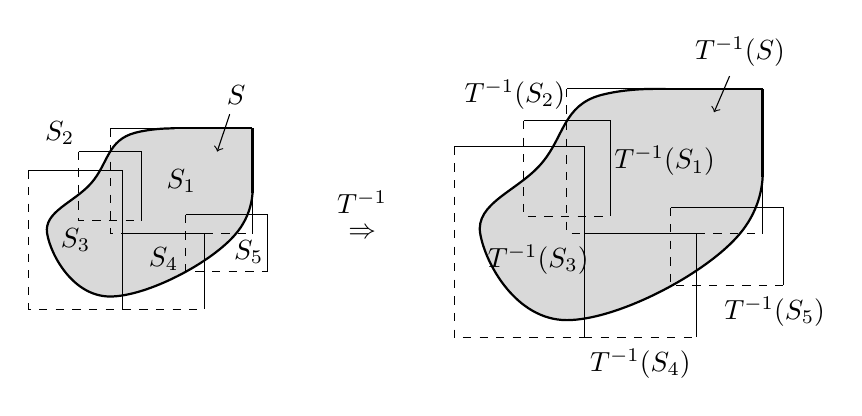
\begin{tikzpicture}
            \begin{scope}[scale = 0.8]
                \begin{scope}[style = thick]
                    \draw[fill = gray!30!white] plot[smooth cycle, tension = 0.7] coordinates{(0,0) (1,-1) (3,0) (3,1.4) (1.4,1.6) (0.7,0.8)};
                    \fill[fill = gray!30!white] (2,1.67) -- (3.26,1.67) -- (3.26,0.65) -- cycle;
                    \draw (2,1.67) -- (3.26,1.67);
                    \draw (3.26,0.65) -- (3.26,1.67);
                \end{scope}
                \draw (1,1.67) -- (3.26,1.67) -- (3.26,0);
                \draw (0.5,1.3) -- (1.5,1.3) -- (1.5,0.2);
                \draw (-0.3,1) -- (1.2,1) -- (1.2,-1.2);
                \draw (1.2,0) -- (2.5,0) -- (2.5,-1.2);
                \draw (2.2,0.3) -- (3.5,0.3) -- (3.5,-0.6);
                \begin{scope}[style = dashed]
                    \draw (1,1.67) -- (1,0) -- (1.2,0);
                    \draw (2.5,0) -- (3.26,0);
                    \draw (0.5,1.3) -- (0.5,0.2) -- (1.5,0.2);
                    \draw (-0.3,1) -- (-0.3,-1.2) -- (1.2,-1.2);
                    \draw (1.2,-1.2) -- (2.5,-1.2);
                    \draw (2.2,0.3) -- (2.2,-0.6) -- (3.5,-0.6);
                \end{scope}
                \node (a) at (3,2.2) {$S$};
                \node at (2.13,0.835) {$S_1$};
                \node at (0.2,1.6) {$S_2$};
                \node at (0.45,-0.1) {$S_3$};
                \node at (1.85,-0.4) {$S_4$};
                \node at (3.2,-0.3) {$S_5$};
                \draw[<-] (2.7,1.3) -- (a);
            \end{scope}
            \node at (4,0) {$\Rightarrow$};
            \node at (4,0.4) {$T^{-1}$};
            \begin{scope}[scale = 1.1, shift = {(5,0)}]
                \begin{scope}[style = thick]
                    \draw[fill = gray!30!white] plot[smooth cycle, tension = 0.7] coordinates{(0,0) (1,-1) (3,0) (3,1.4) (1.4,1.6) (0.7,0.8)};
                    \fill[fill = gray!30!white] (2,1.67) -- (3.26,1.67) -- (3.26,0.65) -- cycle;
                    \draw (2,1.67) -- (3.26,1.67);
                    \draw (3.26,0.65) -- (3.26,1.67);
                \end{scope}
                \draw (1,1.67) -- (3.26,1.67) -- (3.26,0);
                \draw (0.5,1.3) -- (1.5,1.3) -- (1.5,0.2);
                \draw (-0.3,1) -- (1.2,1) -- (1.2,-1.2);
                \draw (1.2,0) -- (2.5,0) -- (2.5,-1.2);
                \draw (2.2,0.3) -- (3.5,0.3) -- (3.5,-0.6);
                \begin{scope}[style = dashed]
                    \draw (1,1.67) -- (1,0) -- (1.2,0);
                    \draw (2.5,0) -- (3.26,0);
                    \draw (0.5,1.3) -- (0.5,0.2) -- (1.5,0.2);
                    \draw (-0.3,1) -- (-0.3,-1.2) -- (1.2,-1.2);
                    \draw (1.2,-1.2) -- (2.5,-1.2);
                    \draw (2.2,0.3) -- (2.2,-0.6) -- (3.5,-0.6);
                \end{scope}
                \node (a) at (3,2.1) {$T^{-1}(S)$};
                \node at (2.13,0.835) {$T^{-1}(S_1)$};
                \node at (0.4,1.6) {$T^{-1}(S_2)$};
                \node at (0.67,-0.3) {$T^{-1}(S_3)$};
                \node at (1.85,-1.5) {$T^{-1}(S_4)$};
                \node at (3.4,-0.9) {$T^{-1}(S_5)$};
                \draw[<-] (2.7,1.4) -- (a);
            \end{scope}
        \end{tikzpicture}
    \end{figure}

    \begin{figure}[ht!]
        \centering
        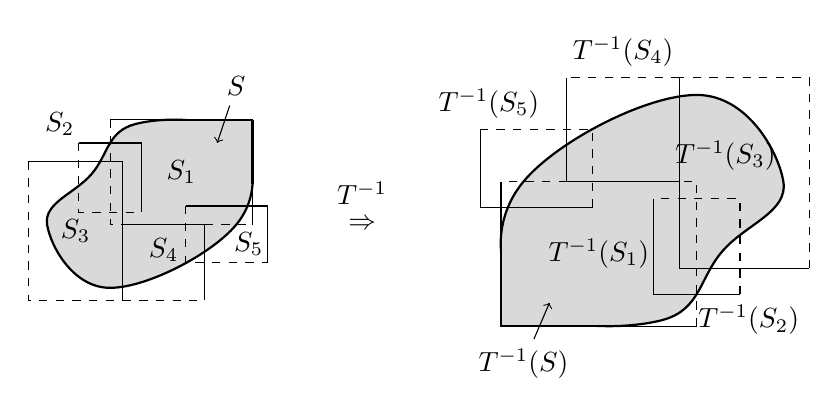
\begin{tikzpicture}
            \begin{scope}[scale = 0.8]
                \begin{scope}[style = thick]
                    \draw[fill = gray!30!white] plot[smooth cycle, tension = 0.7] coordinates{(0,0) (1,-1) (3,0) (3,1.4) (1.4,1.6) (0.7,0.8)};
                    \fill[fill = gray!30!white] (2,1.67) -- (3.26,1.67) -- (3.26,0.65) -- cycle;
                    \draw (2,1.67) -- (3.26,1.67);
                    \draw (3.26,0.65) -- (3.26,1.67);
                \end{scope}
                \draw (1,1.67) -- (3.26,1.67) -- (3.26,0);
                \draw (0.5,1.3) -- (1.5,1.3) -- (1.5,0.2);
                \draw (-0.3,1) -- (1.2,1) -- (1.2,-1.2);
                \draw (1.2,0) -- (2.5,0) -- (2.5,-1.2);
                \draw (2.2,0.3) -- (3.5,0.3) -- (3.5,-0.6);
                \begin{scope}[style = dashed]
                    \draw (1,1.67) -- (1,0) -- (1.2,0);
                    \draw (2.5,0) -- (3.26,0);
                    \draw (0.5,1.3) -- (0.5,0.2) -- (1.5,0.2);
                    \draw (-0.3,1) -- (-0.3,-1.2) -- (1.2,-1.2);
                    \draw (1.2,-1.2) -- (2.5,-1.2);
                    \draw (2.2,0.3) -- (2.2,-0.6) -- (3.5,-0.6);
                \end{scope}
                \node (a) at (3,2.2) {$S$};
                \node at (2.13,0.835) {$S_1$};
                \node at (0.2,1.6) {$S_2$};
                \node at (0.45,-0.1) {$S_3$};
                \node at (1.85,-0.4) {$S_4$};
                \node at (3.2,-0.3) {$S_5$};
                \draw[<-] (2.7,1.3) -- (a);
            \end{scope}
            \node at (4,0) {$\Rightarrow$};
            \node at (4,0.4) {$T^{-1}$};
            \begin{scope}[rotate = -180, scale = 1.1, shift = {(-8.5,-0.5)}]
                \begin{scope}[style = thick]
                    \draw[fill = gray!30!white] plot[smooth cycle, tension = 0.7] coordinates{(0,0) (1,-1) (3,0) (3,1.4) (1.4,1.6) (0.7,0.8)};
                    \fill[fill = gray!30!white] (2,1.67) -- (3.26,1.67) -- (3.26,0.65) -- cycle;
                    \draw (2,1.67) -- (3.26,1.67);
                    \draw (3.26,0.65) -- (3.26,1.67);
                \end{scope}
                \draw (1,1.67) -- (3.26,1.67) -- (3.26,0);
                \draw (0.5,1.3) -- (1.5,1.3) -- (1.5,0.2);
                \draw (-0.3,1) -- (1.2,1) -- (1.2,-1.2);
                \draw (1.2,0) -- (2.5,0) -- (2.5,-1.2);
                \draw (2.2,0.3) -- (3.5,0.3) -- (3.5,-0.6);
                \begin{scope}[style = dashed]
                    \draw (1,1.67) -- (1,0) -- (1.2,0);
                    \draw (2.5,0) -- (3.26,0);
                    \draw (0.5,1.3) -- (0.5,0.2) -- (1.5,0.2);
                    \draw (-0.3,1) -- (-0.3,-1.2) -- (1.2,-1.2);
                    \draw (1.2,-1.2) -- (2.5,-1.2);
                    \draw (2.2,0.3) -- (2.2,-0.6) -- (3.5,-0.6);
                \end{scope}
                \node (a) at (3,2.1) {$T^{-1}(S)$};
                \node at (2.13,0.835) {$T^{-1}(S_1)$};
                \node at (0.4,1.6) {$T^{-1}(S_2)$};
                \node at (0.67,-0.3) {$T^{-1}(S_3)$};
                \node at (1.85,-1.5) {$T^{-1}(S_4)$};
                \node at (3.4,-0.9) {$T^{-1}(S_5)$};
                \draw[<-] (2.7,1.4) -- (a);
            \end{scope}
        \end{tikzpicture}
    \end{figure}

    \begin{figure}[ht!]
        \centering
        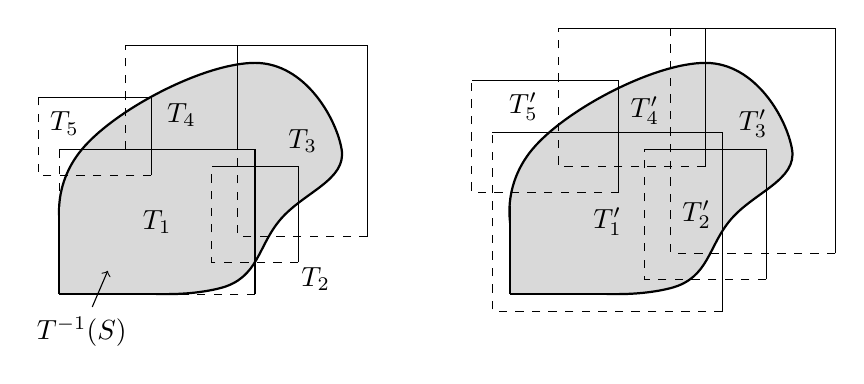
\begin{tikzpicture}
            \begin{scope}[rotate = -180, scale = 1.1]
                \begin{scope}[style = thick]
                    \draw[fill = gray!30!white] plot[smooth cycle, tension = 0.7] coordinates{(0,0) (1,-1) (3,0) (3,1.4) (1.4,1.6) (0.7,0.8)};
                    \fill[fill = gray!30!white] (2,1.67) -- (3.26,1.67) -- (3.26,0.65) -- cycle;
                    \draw (2,1.67) -- (3.26,1.67);
                    \draw (3.26,0.65) -- (3.26,1.67);
                \end{scope}
                \draw (1,1.67) -- (1,0) -- (3.26,0);
                \draw (0.5,1.3) -- (0.5,0.2) -- (1.5,0.2);
                \draw (-0.3,1) -- (-0.3,-1.2) -- (1.2,-1.2);
                \draw (1.2,0) -- (1.2,-1.2) -- (2.5,-1.2);
                \draw (2.2,0.3) -- (2.2,-0.6) -- (3.5,-0.6);
                \begin{scope}[style = dashed]
                    \draw (1,1.67) -- (3.26,1.67) -- (3.26,0);
                    \draw (0.5,1.3) -- (1.5,1.3) -- (1.5,0.2);
                    \draw (-0.3,1) -- (1.2,1) -- (1.2,0);
                    \draw (2.5,0) -- (2.5,-1.2);
                    \draw (2.2,0.3) -- (3.5,0.3) -- (3.5,-0.6);
                \end{scope}
                \node (a) at (3,2.1) {$T^{-1}(S)$};
                \node at (2.13,0.835) {$T_1$};
                \node at (0.3,1.5) {$T_2$};
                \node at (0.45,-0.1) {$T_3$};
                \node at (1.85,-0.4) {$T_4$};
                \node at (3.2,-0.3) {$T_5$};
                \draw[<-] (2.7,1.4) -- (a);
            \end{scope}
            \begin{scope}[rotate = -180, scale = 1.1, shift = {(-5.2,0)}]
                \begin{scope}[style = thick]
                    \draw[fill = gray!30!white] plot[smooth cycle, tension = 0.7] coordinates{(0,0) (1,-1) (3,0) (3,1.4) (1.4,1.6) (0.7,0.8)};
                    \fill[fill = gray!30!white] (2,1.67) -- (3.26,1.67) -- (3.26,0.65) -- cycle;
                    \draw (2,1.67) -- (3.26,1.67);
                    \draw (3.26,0.65) -- (3.26,1.67);
                \end{scope}
                \draw (0.8,1.87) -- (0.8,-0.2) -- (3.46,-0.2);
                \draw (0.3,1.5) -- (0.3,0) -- (1.7,0);
                \draw (-0.5,1.2) -- (-0.5,-1.4) -- (1,-1.4);
                \draw (1,0.2) -- (1,-1.4) -- (2.7,-1.4);
                \draw (2,0.5) -- (2,-0.8) -- (3.7,-0.8);
                \begin{scope}[style = dashed]
                    \draw (0.8,1.87) -- (3.46,1.87) -- (3.46,-0.2);
                    \draw (0.3,1.5) -- (1.7,1.5) -- (1.7,0);
                    \draw (-0.5,1.2) -- (1.4,1.2) -- (1.4,-1.4);
                    \draw (1,0.2) -- (2.7,0.2) -- (2.7,-1.4);
                    \draw (2,0.5) -- (3.7,0.5) -- (3.7,-0.8);
                \end{scope}
                \node at (2.13,0.835) {$T_1'$};
                \node at (1.1,0.75) {$T_2'$};
                \node at (0.45,-0.3) {$T_3'$};
                \node at (1.7,-0.45) {$T_4'$};
                \node at (3.1,-0.5) {$T_5'$};
            \end{scope}
        \end{tikzpicture}
        \caption{변수변환 공식의 증명의 4단계에서의 집합 $S$와 임의의 가산 덮개 $\{S_i\}$가 \texttt{homothety} $T$에 의해 변환되는 모습. 각각 $c>0$인 경우(위)와 $c<0$인 경우(중간). 한편, $c<0$인 경우에는 $\{T_i\}$가 $T^{-1}(S)$의 가산 덮개가 되지 못할 수도 있으므로(왼쪽 아래) 각 $T_i$를 조금씩 늘려 $\{T_i'\}$를 구성한다(오른쪽 아래).}
    \end{figure}

    \noindent\texttt{\textbf{Step 5.}} 모든 가역인 선형사상 $T:\mathbb{R}^n\to\mathbb{R}^n$는 \texttt{good}이다.

    모든 가역인 선형사상은 (표준기저에 대해) 기본행렬로 나타내어지는 유한개의 선형사상의 합성으로 쓸 수 있으므로 2단계로부터 $T$가 다음 3가지와 같은 경우에 대해서만 생각하면 된다.
    \begin{enumerate}
        \item $T:(\cdots,\,x_i,\,\cdots)\mapsto(\cdots,\,cx_i,\,\cdots)$ (단, $c\ne0$이다.)
        \item $T:(\cdots,\,x_i,\,\cdots)\mapsto(\cdots,\,x_i+cx_j,\,\cdots)$
        \item $T:(\cdots,\,x_i,\,\cdots,\,x_j,\,\cdots)\mapsto(\cdots,\,x_j,\,\cdots,\,x_i,\,\cdots)$
    \end{enumerate}

    간결한 논의를 위해 $i=1,\,j=2$인 경우에 대해서만 보이도록 하고, 이하 $f:\mathbb{R}^n\to\overline{\mathbb{R}}^+_0$를 임의의 가측함수라 하자. (다른 $i,\,j$에 대해서도 이와 비슷하게 하면 된다.) 우선 $f\circ T$가 가측임을 보이려고 하는데, 만약 $f$가 \texttt{Borel}이면 정리 \ref{thm:compositionMeasurable}로부터 $f\circ T$가 가측임이 분명하다. 한편, 정리 \ref{thm:LebesgueComplete}와 \ref{thm:measureCompletionApprox}로부터 적당한 \texttt{Borel} 함수 $g:\mathbb{R}^n\to\overline{\mathbb{R}}$가 존재하여 $f=g$ (\texttt{ae.})이다. 이제 $N=\{x\in\mathbb{R}^n:f(x)\ne g(x)\}$라 하면 이가 영집합이고 $T^{-1}$가 \texttt{Lipschitz} 연속이므로 위의 보조정리로부터 $T^{-1}(N)=\{x\in\mathbb{R}^n:(f\circ T)(x)\ne(g\circ T)(x)\}$가 영집합이 되어 $f\circ T=g\circ T$ (\texttt{ae.})이다. 그렇다면 \texttt{Lebesgue} 측도공간이 완비성을 가진다는 사실과 정리 \ref{thm:equalityAeMeasurable}로부터 $f\circ T$도 가측이다.

    다음으로, 위의 세 가지 경우에 대해 $\int_{\mathbb{R}^n}f\,d\lambda_n=\int_{\mathbb{R}^n}(f\circ T)|\det\D T|\,d\lambda_n$임을 보이자. 먼저 첫 번째 경우를 보면 \texttt{Fubini}의 정리와 4단계의 결과로부터
    \begin{align*}
        \int_{\mathbb{R}^n}f\,d\lambda_n&=\int_\mathbb{R}\cdots\int_\mathbb{R}f(x_1,\,\cdots,\,x_n)\,d\lambda_1(x_1)\cdots\,d\lambda_1(x_n)\\
        &=\int_\mathbb{R}\cdots\int_\mathbb{R}f(cx_1,\,\cdots,\,x_n)|c|\,d\lambda_1(x_1)\cdots\,d\lambda_1(x_n)\\
        &=\int_\mathbb{R}\cdots\int_\mathbb{R}(f\circ T)(x_1,\,\cdots,\,x_n)|c|\,d\lambda_1(x_1)\cdots\,d\lambda_1(x_n)\\
        &=\int_{\mathbb{R}^n}(f\circ T)|\det\D T|\,d\lambda_n
    \end{align*}
    이다. 두 번째 경우에도 \texttt{Fubini}의 정리와 3단계의 결과로부터
    \begin{align*}
        \int_{\mathbb{R}^n}f\,d\lambda_n&=\int_\mathbb{R}\cdots\int_\mathbb{R}f(x_1,\,\cdots,\,x_n)\,d\lambda_1(x_1)\cdots\,d\lambda_1(x_n)\\
        &=\int_\mathbb{R}\cdots\int_\mathbb{R}f(x_1+cx_2,\,\cdots,\,x_n)\,d\lambda_1(x_1)\cdots\,d\lambda_1(x_n)\\
        &=\int_\mathbb{R}\cdots\int_\mathbb{R}(f\circ T)(x_1,\,\cdots,\,x_n)\,d\lambda_1(x_1)\cdots\,d\lambda_1(x_n)\\
        &=\int_{\mathbb{R}^n}(f\circ T)|\det\D T|\,d\lambda_n
    \end{align*}
    이며 마지막 경우에도 \texttt{Fubini}의 정리로부터
    \begin{align*}
        \int_{\mathbb{R}^n}f\,d\lambda_n&=\int_\mathbb{R}\cdots\int_\mathbb{R}f(x_1,\,x_2,\,\cdots,\,x_n)\,d\lambda_1(x_2)\,d\lambda_1(x_1)\cdots\,d\lambda_1(x_n)\\
        &=\int_\mathbb{R}\cdots\int_\mathbb{R}f(x_2,\,x_1,\,\cdots,\,x_n)\,d\lambda_1(x_1)\,d\lambda_1(x_2)\cdots\,d\lambda_1(x_n)\\
        &=\int_\mathbb{R}\cdots\int_\mathbb{R}(f\circ T)(x_1,\,\cdots,\,x_n)\,d\lambda_1(x_1)\,d\lambda_1(x_2)\cdots\,d\lambda_1(x_n)\\
        &=\int_{\mathbb{R}^n}(f\circ T)|\det\D T|\,d\lambda_n
    \end{align*}
    이다. 이상으로부터 어느 경우에나 $T$가 \texttt{good}이 되어 임의의 가역인 선형사상이 \texttt{good}임을 안다.

    2단계, 3단계, 5단계의 결과를 종합하면 임의의 \texttt{Affine} 변환이 \texttt{good}임을 안다. 이제 증명의 후반부를 위해 임의의 $\mathcal{C}^1$급 미분동형사상 $\Phi:U\to V$와 임의의 \texttt{compact}한 $K\subseteq U$를 고정하고, $\mathbb{R}^n$에 최대값 노름 $||\cdot||_\infty$를 장착하자.

    \noindent\texttt{\textbf{Step 6.}} 임의의 $\epsilon>0$에 대해 적당한 $\delta>0$가 존재하여 임의의 $x,\,y\in K$가 $||x-y||_\infty<\delta$와 $\prod_{i=1}^n[x_i,\,y_i]\subseteq K$를 만족하면 $||\Phi(x)-\Phi(y)-\D\Phi(x)(y-x)||_\infty<\epsilon||x-y||_\infty$이다.

    편의를 위해 $\prod_{i=1}^n[x_i,\,y_i]\subseteq K$를 만족하는 임의의 $x,\,y\in K$를 고정하자. 이제 함수 $\gamma:[0,\,1]\to\mathbb{R}^n$를 $\gamma:t\mapsto\Phi((1-t)x+ty)$로 두면 이는 $\mathcal{C}^1$급이고, \texttt{FTC}로부터 $\Phi(y)-\Phi(x)=\int_0^1\nabla\gamma=\int_0^1\D\Phi((1-t)x+ty)(y-x)\,dt$이다. 이로부터 함수 $\Gamma:[0,\,1]\to\mathsf{L}(\mathbb{R}^n,\,\mathbb{R}^n)$를 $\Gamma:t\mapsto\D\Phi((1-t)x+ty)-\D\Phi(x)$로 두면 $\Phi(y)-\Phi(x)=\int_0^1\D\Phi((1-t)x+ty)(y-x)\,dt=\int_0^1[\D\Phi(x)+\Gamma(t)](y-x)\,dt=\D\Phi(x)(y-x)+\int_0^1\Gamma(t)(y-x)\,dt$이다. 한편, $\D\Phi:\mathbb{R}^n\to\mathsf{L}(\mathbb{R}^n,\,\mathbb{R}^n)$가 $K$ 위에서 균등연속이므로 임의의 $\epsilon>0$을 택하면 적당한 $\delta>0$가 존재하여 $||x-y||_\infty<\delta$이면 $||\D\Phi(x)-\D\Phi(y)||_\mathrm{op}<\epsilon$이다. 이제 $||x-y||_\infty<\delta$라 하고 임의의 $t\in[0,\,1]$에 대해 $z=(1-t)x+ty$라 하면 $||x-z||_\infty\leq||x-y||_\infty<\delta$에서 $||\Gamma(t)||_\mathrm{op}=||\D\Phi(x)-\D\Phi(z)||_\mathrm{op}<\epsilon$이 되어 이상으로부터 각 $i\leq n$에 대해 $\int_0^1\Gamma_i(t)(y-x)\,dt\leq\int_0^1||\Gamma(t)(y-x)||_\infty\,dt\leq\int_0^1||\Gamma(t)||_\mathrm{op}||x-y||_\infty\,dt<\epsilon||x-y||_\infty$이므로 곧 $||\Phi(x)-\Phi(y)-\D\Phi(x)(y-x)||_\infty=||\int_0^1\Gamma(t)(y-x)\,dt||_\infty<\epsilon||x-y||_\infty$가 성립한다.

    이제 임의의 $x\in U$에 대해 함수 $\Psi_x:\mathbb{R}^n\to\mathbb{R}^n$를 $\Psi_x:y\mapsto\Phi(x)+\D\Phi(x)(x-y)$로 두면 이는 \texttt{Affine} 변환이며 곧 \texttt{good}이다. 나아가 6단계의 결과로부터 임의의 $\epsilon>0$에 대해 적당한 $\delta>0$가 존재하여 임의의 $x,\,y\in K$가 $||x-y||_\infty<\delta$와 $\prod_{i=1}^n[x_i,\,y_i]\subseteq K$를 만족하면 $||\Phi(y)-\Psi_{x}(y)||_\infty<\epsilon||x-y||_\infty$이다.

    \noindent\texttt{\textbf{Step 7.}} 임의의 $0<\epsilon<1$에 대해 적당한 $\delta>0$가 존재하여 임의의 열린 \texttt{ball} $B(x,\,r)\subseteq K$이 $r<\delta$를 만족하면 $\Psi_x(B(x,\,(1-\epsilon)r))\subseteq\Phi(B(x,\,r))\subseteq\Psi_x(B(x,\,(1+\epsilon)r))$이다.

    미분동형사상 $\Phi$가 $\mathcal{C}^1$급이고 집합 $K$가 \texttt{compact}하여 $(\D\Phi(\cdot))^{-1}:K\to\mathsf{L}(\mathbb{R}^n,\,\mathbb{R}^n)$가 유계이므로 $M:=\sup_{x\in K}||(\D\Phi(x))^{-1}||_\mathrm{op}<\infty$이다. 그렇다면 임의의 $x\in K$와 임의의 $y,\,z\in\mathbb{R}^n$에 대해 $\Psi_x^{-1}(y)=(\D\Phi(x))^{-1}(\Phi(x)-y)+x$이고, 이는 $z$에 대해서도 마찬가지이므로 $||\Psi_x^{-1}(y)-\Psi_x^{-1}(z)||_\infty=||(\D\Phi(x))^{-1}(y-z)||_\infty\leq||(\D\Phi(x))^{-1}||_\mathrm{op}||y-z||_\infty\leq M||y-z||_\infty$이다. 이제 임의의 $x\in K^\circ$를 고정하고 임의의 $0<\epsilon<1$을 택하면 적당한 $\delta>0$가 존재하여 임의의 $y\in K$가 $||x-y||_\infty<\delta$와 $\prod_{i=1}^n[x_i,\,y_i]\subseteq K$를 만족하면 $||\Phi(y)-\Psi_x(y)||_\infty<[\epsilon/(M+1)]||x-y||_\infty$이다. 이러한 $\delta$에 대해 임의의 $r<\delta$도 고정하되, \texttt{WLOG}, 필요하다면 $r$을 더 작게 하여 $B(x,\,r)\subseteq K$라 하면 임의의 $y\in B(x,\,r)$에 대해 $||x-y||_\infty<r<\delta$이고 $\prod_{i=1}^n[x_i,\,y_i]\subseteq B(x,\,r)\subseteq K$가 되어 $||\Phi(y)-\Psi_x(y)||_\infty<[\epsilon/(M+1)]||x-y||_\infty<\epsilon r/(M+1)$이다. 이상을 종합하면 임의의 $y\in B(x,\,r)$에 대해 $||(\Psi_x^{-1}\circ\Phi)(y)-y||_\infty=||(\Psi_x^{-1}\circ\Phi)(y)-(\Psi_x^{-1}\circ\Psi_x)(y)||_\infty\leq M||\Phi(y)-\Psi_x(y)||_\infty<\epsilon r$이 성립하여 $||(\Psi_x^{-1}\circ\Phi)(y)-x||_\infty\leq||(\Psi_x^{-1}\circ\Phi)(y)-y||_\infty+||x-y||_\infty<(1+\epsilon)r$이므로 $\Phi(y)\in\Psi_x(B(x,\,(1+\epsilon)r))$이고, 곧 $\Phi(B(x,\,r))\subseteq\Psi_x(B(x,\,(1+\epsilon)r))$임을 안다.

    다른 포함관계를 보이기 위해 $x\in K$와 $r>0$, $0<\epsilon<1$을 위에서와 같이 두고 임의의 $y\in S(x,\,r)$를 생각하면 $||x-y||_\infty=r$이므로 $||(\Psi_x^{-1}\circ\Phi)(y)-x||_\infty\geq||x-y||_\infty-||(\Psi_x^{-1}\circ\Phi)(y)-y||_\infty>(1-\epsilon)r$에서 $\Phi(y)\notin\Psi_x(B(x,\,(1-\epsilon)r))$이다. 이는 곧 $\Psi_x(B(x,\,(1-\epsilon)r))$과 $\Phi(S(x,\,r))$이 서로소임을 뜻하므로 집합 $A=\Psi_x(B(x,\,(1-\epsilon)r))\cap\Phi(B(x,\,r)),\,B=\Psi_x(B(x,\,(1-\epsilon)r))\setminus\Phi(B(x,\,r))$를 생각하면 $A\sqcup B=\Psi_x(B(x,\,(1-\epsilon)r))$이며 $A$는 열린집합임이 자명하고 $B=\Psi_x(B(x,\,(1-\epsilon)r))\setminus[\Phi(B(x,\,r))\cup\Phi(S(x,\,r))]=\Psi_x(B(x,\,(1-\epsilon)r))\setminus\Phi(\overline{B(x,\,r)})$에서 $B$도 열린집합이다.\footnotemark 그러나 $\Psi_x(B(x,\,(1-\epsilon)r))$이 연결집합이므로 $A,\,B$ 중 하나는 공집합인데, $\Psi_x(x)=\Phi(x)\in A$이므로 $B=\emptyset$이 되어 $A=\Psi_x(B(x,\,(1-\epsilon)r))$이고, 곧 $\Psi_x(B(x,\,(1-\epsilon)r))\subseteq\Phi(B(x,\,r))$이 되어 7단계의 증명이 끝난다.

    \noindent\texttt{\textbf{Step 8.}} 가측집합 $A\subseteq U$에 대해 $\Phi(A)$도 가측이다.

    함수 $\Phi$가 미분동형사상이므로 $\Phi^{-1}$가 연속이고, 곧 가측이므로 임의의 \texttt{Borel} 집합 $B\subseteq U$에 대해 $\Phi(B)=(\Phi^{-1})^{-1}(B)$가 가측이다. 한편, 정리 \ref{thm:Complete2}, \ref{thm:LebesgueComplete}로부터 임의의 가측집합 $A\subseteq U$에 대해 적당한 \texttt{Borel} 집합 $B,\,C\subseteq\mathbb{R}^n$가 존재하여 $B\subseteq A\subseteq C$이며 $C\setminus B$가 영집합이고, $C\setminus A\subseteq C\setminus B$이므로 $N:=C\setminus A$도 영집합이다. 나아가 \texttt{WLOG}, 필요하다면 $B,\,C$를 각각 $B\cap U,\,C\cap U$로 바꾸어 $B,\,C\subseteq U$라 해도 된다. 그렇다면 $\Phi(A)=\Phi(C)\setminus\Phi(N)$에서 $\Phi(C)$는 앞선 결과로부터 가측이고, $\Phi(N)$은 위의 보조정리로부터 영집합이 되어 \texttt{Lebesgue} 측도공간이 완비성을 가진다는 점에서 곧 가측이므로 $\Phi(A)$는 가측이다.

    \noindent\texttt{\textbf{Step 9.}} 열린집합 $W\subseteq U$에 대해 $\lambda_n(\Phi(W))=\int_W|\det\D\Phi|\,d\lambda_n$이다.

    먼저 $W\subseteq K$인 특별한 경우를 생각하자. 임의의 $\epsilon>0$을 택하고 $k\geq1$를 충분히 크게 잡으면 $\log|\det\D\Phi(\cdot)|:K\to\mathbb{R}$가 균등연속이므로 적당한 $\delta>0$가 존재하여 임의의 $x,\,y\in K$가 $||x-y||_\infty<\delta$를 만족하면 $|\log|\det\D\Phi(x)/\det\D\Phi(y)||=|\log|\det\D\Phi(x)|-\log|\det\D\Phi(y)||<\epsilon/k$이고 곧 $1-\epsilon\leq1-\epsilon/k\leq e^{-\epsilon/k}<|\det\D\Phi(x)/\det\D\Phi(y)|<e^{\epsilon/k}\leq1+\epsilon$이다. 또한, 7단계의 결과로부터 \texttt{WLOG}, 필요하다면 $\delta>0$를 더 작게 하여 임의의 열린 \texttt{ball} $B(x,\,r)\subseteq K$이 $r<\delta$를 만족하면 $\Psi_x(B(x,\,(1-\epsilon)r))\subseteq\Phi(B(x,\,r))\subseteq\Psi_x(B(x,\,(1+\epsilon)r))$이도록 할 수 있다. 나아가, $\mathcal{P}(W)$에 속하는 적당한 서로소인 열린 \texttt{ball}의 열 $\{B(x_i,\,r_i)\}$가 존재하여 각 $i\in\mathbb{N}$에 대해 $r_i<\delta$이고 $\lambda_n(W\setminus\bigsqcup_{i=1}^\infty B(x_i,\,r_i))=0$이며,\footnotemark\label{note:countableBoundaryNull} 위의 보조정리로부터 $\lambda_n(\Phi(W)\setminus\bigsqcup_{i=1}^\infty\Phi(B(x_i,\,r_i)))=\lambda_n(\Phi(W\setminus\bigsqcup_{i=1}^\infty B(x_i,\,r_i)))=0$이다. 이상을 종합하면 \texttt{Affine} 변환이 \texttt{good}이라는 점과 따름정리 \ref{cor:zeroAeIntegral}, 정리 \ref{thm:monoSeriesIntegral}로부터 각 $i\in\mathbb{N}$에 대해
    \begin{align*}
        \lambda_n(\Psi_{x_i}(B(x_i,\,(1+\epsilon)r_i)))&=\int_{B(x_i,\,(1+\epsilon)r_i)}|\det\D\Psi_{x_i}|\,d\lambda_n\\
        &=|\det\D\Phi(x_i)|\lambda_n(B(x_i,\,(1+\epsilon)r_i))\\
        &=|\det\D\Phi(x_i)|(1+\epsilon)^n\lambda_n(B(x_i,\,r_i))\\
        &\leq(1+\epsilon)^{n+1}\int_{B(x_i,\,r_i)}|\det\D\Phi|\,d\lambda_n
    \end{align*}
    이고, 이로부터
    \begin{align*}
        \lambda_n(\Phi(W))&=\lambda_n\bigg(\bigsqcup_{i=1}^\infty\Phi(B(x_i,\,r_i))\bigg)\\
        &=\sum_{i=1}^\infty\lambda_n(\Phi(B(x_i,\,r_i)))\\
        &\leq\sum_{i=1}^\infty\lambda_n(\Psi_{x_i}(B(x_i,\,(1+\epsilon)r_i)))\\
        &\leq(1+\epsilon)^{n+1}\sum_{i=1}^\infty\int_{B(x_i,\,r_i)}|\det\D\Phi|\,d\lambda_n\\
        &=(1+\epsilon)^{n+1}\int_{\bigsqcup_{i=1}^\infty B(x_i,\,r_i)}|\det\D\Phi|\,d\lambda_n\\
        &=(1+\epsilon)^{n+1}\int_W|\det\D\Phi|\,d\lambda_n
    \end{align*}
    이다. 이제 $(1-\epsilon)^{n+1}\int_W|\det\D\Phi|\,d\lambda_n\leq\lambda_n(\Phi(W))$임을 이와 비슷하게 보일 수 있으므로 곧 $\lambda_n(\Phi(W))=\int_W|\det\D\Phi|\,d\lambda_n$임을 안다.

    이제 일반적인 $W\subseteq K$에 대해 $\mathcal{P}(U)$에 속하는 적당한 서로소인 열린 \texttt{ball}의 열 $\{B_i\}$가 존재하여 각 $i\in\mathbb{N}$에 대해 $\overline{B_i}\subseteq U$이고 $\lambda_n(U\setminus\bigsqcup_{i=1}^\infty B_i)=0$이다.\footnotemark 따라서 위의 보조정리로부터 $\lambda_n(\Phi(W)\setminus\bigsqcup_{i=1}^\infty\Phi(W\cap B_i))=\lambda_n(\Phi(W\setminus\bigsqcup_{i=1}^\infty B_i))\leq\lambda_n(\Phi(U\setminus\bigsqcup_{i=1}^\infty B_i))=0$이고, 각 $i\in\mathbb{N}$에 대해 $W\cap B_i\subseteq\overline{B_i}\subseteq U$이므로 앞선 결과에서 $K\subseteq U$가 임의의 \texttt{compact}한 집합이었음을 상기한다면
    \begin{align*}
        \lambda_n(\Phi(W))&=\lambda_n\bigg(\bigsqcup_{i=1}^\infty\Phi(W\cap B_i)\bigg)\\
        &=\sum_{i=1}^\infty\lambda_n(\Phi(W\cap B_i))\\
        &=\sum_{i=1}^\infty\int_{W\cap B_i}|\det\D\Phi|\,d\lambda_n\\
        &=\int_{\bigsqcup_{i=1}^\infty(W\cup B_i)}|\det\D\Phi|\,d\lambda_n\\
        &=\int_W|\det\D\Phi|\,d\lambda_n
    \end{align*}
    이다.

    \noindent\texttt{\textbf{Step 10.}} 닫힌집합 $F\subseteq U$에 대해 $\lambda_n(\Phi(F))=\int_F|\det\D\Phi|\,d\lambda_n$이다.

    만약 $\Phi(F)$가 유계라면 적당한 열린집합 $W\subseteq U$가 존재하여 $\Phi(W)$가 유계이며 $\Phi(F)\subseteq\Phi(W)$이고,\footnotemark 9단계의 결과로부터 $\lambda_n(\Phi(W\setminus F))=\int_{W\setminus F}|\det\D\Phi|\,d\lambda_n<\infty$이고 $\lambda_n(\Phi(W))=\int_W|\det\D\Phi|\,d\lambda_n<\infty$이므로
    \begin{align*}
        \lambda_n(\Phi(F))&=\lambda_n(\Phi(W))-\lambda_n(\Phi(W\setminus F))\\
        &=\int_W|\det\D\Phi|\,d\lambda_n-\int_{W\setminus F}|\det\D\Phi|\,d\lambda_n\\
        &=\int_F|\det\D\Phi|\,d\lambda_n
    \end{align*}
    이다. 이제 $\Phi(F)$가 유계가 아닌 경우에는 집합열 $\{F_i\}$를 $F_i:=F\cap\Phi^{-1}(B(i))$로 두면 각 $i\in\mathbb{N}$에 대해 $\Phi(F_i)=\Phi(F)\cap B(i)$에서 $\Phi(F_i)$는 유계이고, $F_i\uparrow F$임이 자명하다. 한편, $\Phi(F_i)\uparrow\Phi(F)$임도 분명하므로 앞선 결과와 정리 \ref{thm:monoSeriesMeasure}의 i, \ref{thm:monoSeriesIntegral}의 i로부터 $\lambda_n(\Phi(F))=\lim_{i\to\infty}\lambda_n(\Phi(F_i))=\lim_{i\to\infty}\int_{F_i}|\det\D\Phi|\,d\lambda_n=\int_F|\det\D\Phi|\,d\lambda_n$이다.

    증명을 끝내기 위해, 임의의 가측집합 $A\subseteq U$를 생각하면 \texttt{Lebesgue} 측도가 \texttt{regular}하므로
    \begin{align*}
        \lambda_n(\Phi(A))&=\inf\{\lambda_n(W)\in\overline{\mathbb{R}}^+_0:\Phi(A)\subseteq W\subseteq\mathbb{R}^n,\,W\textrm{는 열린집합}\}\\
        &=\inf\{\lambda_n(\Phi(W))\in\overline{\mathbb{R}}^+_0:A\subseteq W\subseteq U,\,W\textrm{는 열린집합}\}\\
        &=\inf\bigg\{\int_W|\det\D\Phi|\,d\lambda_n\in\overline{\mathbb{R}}^+_0:A\subseteq W\subseteq U,\,W\textrm{는 열린집합}\bigg\}\\
        &\geq\int_A|\det\D\Phi|\,d\lambda_n
    \end{align*}
    이고 비슷하게
    \begin{align*}
        \lambda_n(\Phi(A))&=\sup\{\lambda_n(K)\in\overline{\mathbb{R}}^+_0:K\subseteq\Phi(A),\,K\textrm{는 \texttt{compact} 집합}\}\\
        &=\sup\{\lambda_n(\Phi(K))\in\overline{\mathbb{R}}^+_0:K\subseteq A,\,K\textrm{는 \texttt{compact} 집합}\}\\
        &=\sup\bigg\{\int_K|\det\D\Phi|\,d\lambda_n\in\overline{\mathbb{R}}^+_0:K\subseteq A,\,K\textrm{는 \texttt{compact} 집합}\bigg\}\\
        &\leq\int_A|\det\D\Phi|\,d\lambda_n
    \end{align*}
    이 되어 곧 $\lambda_n(\Phi(A))=\int_A|\det\D\Phi|\,d\lambda_n$이다. 이제 1단계와 8단계로부터 임의의 $\mathcal{C}^1$급 미분동형사상이 \texttt{good}임을 안다.

    한편, $V$에서 적분가능한 $f:\mathbb{R}^n\to\overline{\mathbb{R}}$의 경우에는 이를 각각 양과 음의 부분으로 나누어 앞선 결과를 적용하면 $(f\circ\Phi)|\det\D\Phi|$는 $U$에서 적분가능하며 $\int_Vf\,d\lambda_n=\int_U(f\circ\Phi)|\det\D\Phi|\,d\lambda_n$임을 쉽게 알 수 있고, $(f\circ\Phi)|\det\D\Phi|$가 $U$에서 적분가능한 $f:\mathbb{R}^n\to\overline{\mathbb{R}}$에 대해서도 비슷하게 하면 된다.
\end{proof}

여기서 한 발 더 나아가 \texttt{Sard}의 정리와 \texttt{INFT}로부터 변수변환 공식에서의 $\Phi$의 조건을 $\mathcal{C}^1$급 전단사함수로 완화할 수 있다.

\begin{theorem}[Sard]
    열린집합 $U\subseteq\mathbb{R}^n$에서 정의된 $\mathcal{C}^1$급 단사함수 $f:U\to\mathbb{R}^n$의 모든 임계점의 집합 $C$에 대해 $f(C)$는 영집합이다.
\end{theorem}

\begin{proof}
    먼저 $U=(0,\,1)^n$인 특별한 경우를 생각하자. 가정으로부터 $f$가 $\mathcal{C}^1$급이므로 곧 \texttt{Lipschitz} 연속이며, 이때의 \texttt{Lipschitz} 상수를 $L>0$이라 하고 임의의 $x\in U$에 대해 함수 $T_x:\mathbb{R}^n\to\mathbb{R}^n$를 $T_x:y\mapsto f(x)+\D f(x)(y-x)$로 두자. 증명은 크게 2단계로 이루어진다.

    \noindent\textbf{\texttt{Step 1.}} 임의의 $x,\,y\in U$에 대해 $||f(y)-T_x(y)||=o(||x-y||)$이다.

    서로다른 $x,\,y\in U$를 임의로 택하면 \texttt{MVT}에서 $x$와 $y$를 잇는 선분 위에 적당한 $z_1$, $\cdots,\,z_n\in U$이 존재하여 각 $i\leq n$에 대해 $f_i(y)-T_x^i(y)=f_i(y)-f_i(x)-\D f_i(x)(y-x)=[\D f_i(z_i)-\D f_i(x)](y-x)$이다. 이는 각 $i\leq n$에 대해 $|f_i(y)-T_x^i(y)|=|[\D f_i(z_i)-\D f_i(x)](y-x)|\leq||\D f_i(z_i)-\D f_i(x)||_\mathrm{op}||x-y||$임을 뜻하므로 $||f(y)-T_x(y)||/||x-y||\leq\sum_{i=1}^n|f_i(y)-T_x^i(y)|/||x-y||\leq\sum_{i=1}^n||\D f_i(z_i)-\D f_i(x)||_\mathrm{op}$이고, 곧 $f$가 $\mathcal{C}^1$급이라는 사실로부터 $||f(y)-T_x(y)||=o(||x-y||)$임을 안다.

    \noindent\textbf{\texttt{Step 2.}} 임의의 $\epsilon>0$에 대해 적당한 $R>0$이 존재하여 임의의 $0<r<R$에 대해 다음이 성립한다: 임의의 $x\in C$에 대해 적당한 \texttt{box} $B\subseteq\mathbb{R}^n$가 존재하여 $\lambda_n(B)=\epsilon r^n$이고 $f(B(x,\,r))\subseteq B$이다.

    1단계의 결과로부터 적당한 $R>0$이 존재하여 $0<r<R$이면 $||x-y||<r$인 임의의 $x,\,y\in U$에 대해 $||f(y)-T_x(y)||\leq(\epsilon/L^{n-1})||x-y||<\epsilon r/L^{n-1}$이며 $||f(x)-f(y)||<L||x-y||<Lr$이다. 이제 임의의 $x\in C$를 택하면 적당한 $n-1$차원 부분공간 $\mathsf{V}<\mathbb{R}^n$가 존재하여 $\mathrm{im}\,T_x\leq\mathsf{V}$이고, 곧 $||x-y||<r$인 임의의 $y\in U$에 대해 $d(f(y),\,\mathsf{V})\leq||f(y)-T_x(y)||<\epsilon r/L^{n-1}$이다. 따라서 $f(x)$를 중심으로 하고 각 모서리의 길이가 $Lr$로 같은 $n-1$차원 \texttt{box} $B'\subseteq\mathsf{V}$와 이를 $\mathsf{V}$에 수직인 방향으로 $\pm\epsilon r/2L^{n-1}$씩 평행이동시켜 얻는 $n$차원 \texttt{box} $B\subseteq\mathbb{R}^n$를 생각하면 임의의 $y\in B(x,\,r)\cap U$에 대해 $f(y)\in B$임이 자명하여 곧 $f(B(x,\,r))\subseteq B$이고 이때 $\lambda_n(B)=\epsilon r^n$이다. (이는 적당한 \texttt{Affine} 변환에 변수변환 공식을 적용한 결과로, 직관적으로도 자명하다. 이제부터는 이 정도의 변수변환 공식의 가벼운 응용은 특별한 언급 없이 사용하도록 한다.)

    \begin{figure}[ht!]
        \centering
        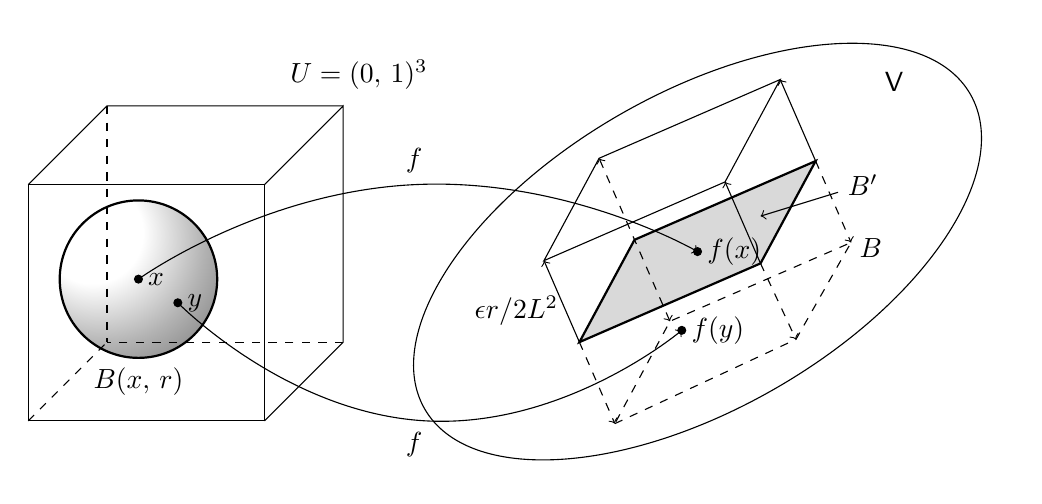
\begin{tikzpicture}
            \draw[rotate around = {-60:(1.5,1.15)}] (1.5,1.15) ellipse (2 and 4);
            \draw[style = thick, fill = gray!30!white] (0,0) -- (2.3,1) -- (3,2.3) -- (0.7,1.3) -- cycle;
            \draw (-0.45,1.035) -- (2.3-0.45,2.035) -- (3-0.45,2.3+1.035) -- (0.7-0.45,1.3+1.035) -- cycle;
            \draw[->] (0,0) -- (-0.45,1.035);
            \draw[->] (2.3,1) -- (2.3-0.45,2.035);
            \draw[->] (3,2.3) -- (3-0.45,2.3+1.035);
            \begin{scope}[style = dashed]
                \draw (0.45,-1.035) -- (2.3+0.45,0.035) -- (3+0.45,2.3-1.035) -- (0.7+0.45,1.3-1.035) -- cycle;
                \draw[<->] (0.7+0.45,1.3-1.035) -- (0.7-0.45,1.3+1.035);
                \draw[->] (0,0) -- (0.45,-1.035);
                \draw[->] (2.3,1) -- (2.3+0.45,0.035);
                \draw[->] (3,2.3) -- (3+0.45,2.3-1.035);
            \end{scope}
            \draw[fill = black] (1.5,1.15) circle[radius = 0.05] node[right] {$f(x)$};
            \draw[fill = black] (1.3,0.15) circle[radius = 0.05] node[right] {$f(y)$};
            \node at (4,3.3) {$\mathsf{V}$};
            \node at (3.7,1.2) {$B$};
            \node (a) at (3.6,2) {$B'$};
            \draw[<-] (2.3,1.6) -- (a);
            \node at (-0.8,0.4) {$\epsilon r/2L^2$};
            \begin{scope}
                \clip (-5.6,0.8) circle[radius = 1];
                \shade[ball color = white] (-5.6,0.8) circle (1.8);
            \end{scope}
            \draw[style = thick] (-5.6,0.8) circle[radius = 1];
            \draw[fill = black] (-5.6,0.8) circle[radius = 0.05] node[right] {$x$};
            \draw[fill = black] (-5.1,0.5) circle[radius = 0.05] node[right] {$y$};
            \draw (-7,-1) -- (-4,-1) -- (-4,2) -- (-7,2) -- cycle;
            \draw (-4,-1) -- (-3,0) -- (-3,3) -- (-4,2);
            \draw (-3,3) -- (-6,3) -- (-7,2);
            \begin{scope}[style = dashed]
                \draw (-7,-1) -- (-6,0);
                \draw (-3,0) -- (-6,0);
                \draw (-6,3) -- (-6,0);
            \end{scope}
            \draw[->] plot[smooth, tension = 1] coordinates{(-5.6,0.8) (-2.1,2) (1.5,1.15)};
            \draw[->] plot[smooth, tension = 1] coordinates{(-5.1,0.5) (-1.95,-1) (1.3,0.15)};
            \node at (-2.8,3.4) {$U=(0,\,1)^3$};
            \node at (-5.6,-0.5) {$B(x,\,r)$};
            \node at (-2.1,2.3) {$f$};
            \node at (-2.1,-1.3) {$f$};
        \end{tikzpicture}
        \caption{\texttt{Sard}의 정리의 증명에서의 집합 $B'$와 $B$.}
    \end{figure}

    증명을 끝내기 위해 임의의 $\epsilon>0$을 택하면 2단계의 결과로부터 적당한 $0<r<1$이 존재하여 다음이 성립한다: 임의의 $x\in C$에 대해 적당한 \texttt{box} $B\subseteq\mathbb{R}^n$가 존재하여 $\lambda_n(B)=\epsilon r^n/(\sqrt{n}+1)^n$이고 $f(B(x,\,r))\subseteq B$이다. 이제 $N=\lceil\sqrt{n}/r\rceil$과 임의의 $j_1,\,\cdots$, $j_n\leq N$에 대해 $B_{j_1\cdots j_n}=\prod_{i=1}^n((j_i-1)/N,\,j_i/N)$라 하고, 이 중에 $C$의 원소를 적어도 하나 포함하는 것만을 택하여 $B_1,\,\cdots,\,B_k$ ($k\leq N^n$)라 하자. 그렇다면 각 $j\leq k$에 대해 $x_j\in B_j\cap C$를 택할 수 있으므로 적당한 \texttt{box} $\widetilde{B}_j\subseteq\mathbb{R}^n$가 존재하여 $\lambda_n(\widetilde{B}_j)=\epsilon r^n/(\sqrt{n}+1)^n$이고 $B_j\subseteq B(x_j,\,\sqrt{n}/N)\subseteq B(x_j,\,r)$에서 $f(B_j)\subseteq f(B(x_j,\,r))\subseteq \widetilde{B}_j$이다. 이제 $f(C)\subseteq\bigcup_{j=1}^kf(B_j)\cup\bigcup_{j_1,\,\cdots,\,j_n=1}^Nf(\partial B_{j_1\cdots j_n})\subseteq\bigcup_{j=1}^k\widetilde{B}_j\cup\bigcup_{j_1,\,\cdots,\,j_n=1}^Nf(\partial B_{j_1\cdots j_n})$인데, 보조정리 \ref{lem:ReimannIntegrable}, \ref{lem:LipschitzNull}에서 $\bigcup_{j_1,\,\cdots,\,j_n=1}^Nf(\partial B_{j_1\cdots j_n})$가 영집합이므로
    \begin{align*}
        \rho_n^*(f(C))&\leq\lambda_n\bigg(\bigcup_{j=1}^k\widetilde{B}_j\cup \bigcup_{j_1,\,\cdots,\,j_n=1}^Nf(\partial B_{j_1\cdots j_n})\bigg)\\
        &\leq\lambda_n\bigg(\bigcup_{j=1}^k\widetilde{B}_j\bigg)\\
        &\leq\sum_{j=1}^k\lambda_n(\widetilde{B}_j)\\
        &=\sum_{j=1}^k\frac{\epsilon r^n}{(\sqrt{n}+1)^n}\\
        &\leq N^n\frac{\epsilon r^n}{(\sqrt{n}+1)^n}\\
        &<\bigg(\frac{\sqrt{n}}{r}+1\bigg)^n\frac{\epsilon r^n}{(\sqrt{n}+1)^n}\\
        &=\bigg(\frac{\sqrt{n}+r}{\sqrt{n}+1}\bigg)^n\epsilon\\
        &<\epsilon
    \end{align*}
    에서 $\rho_n^*(f(C))=0$이다. 이는 곧 임의의 $S\subseteq\mathbb{R}^n$에 대해 $\rho_n^*(S\cap f(C))+\rho_n^*(S\cap[f(C)]^c)\leq\rho_n^*(f(C))+\rho_n^*(S\cap[f(C)]^c)=\rho_n^*(S\cap[f(C)]^c)\leq\rho_n^*(S)$임을 뜻하여 명제 \ref{prop:measurable}로부터 $f(C)$가 영집합임을 안다.

    이제 $f$를 적당히 \texttt{scaling}하고 평행이동함으로써 이상의 결론이 $U$가 임의의 유계인 열린 \texttt{box}인 경우에도 성립함을 알 수 있다. 한편, 일반적인 열린집합 $U\subseteq\mathbb{R}^n$를 생각하면 이는 적당한 유계인 열린 \texttt{box} $B_1,\,B_2,\,\cdots$에 대해 $U=\bigcup_{i=1}^kB_i$로 표현되므로 (각주 \ref{note:countableOpenBox} 참조.) $f(C)=f(\bigcup_{i=1}^k(C\cap B_i))=\bigcup_{i=1}^kf(C\cap B_i)=\bigcup_{i=1}^kf\vert_{B_i}(C)$에서 $f(C)$가 영집합임을 안다. (여기서 $k$는 유한할 수도, $\infty$일 수도 있다.)
\end{proof}

\begin{corollary}[Transformation formula]
    열린집합 $U,\,V\subseteq\mathbb{R}^n$ 사이에서 정의된 $\mathcal{C}^1$급 전단사함수 $\Phi:U\to V$와 음이 아닌 가측함수 $f:\mathbb{R}^n\to\overline{\mathbb{R}}^+_0$에 대해 $(f\circ\Phi)|\det\D\Phi|:U\to\overline{\mathbb{R}}^+_0$는 가측이고 $\int_V f\,d\lambda_n=\int_U(f\circ\Phi)|\det\D\Phi|\,d\lambda_n$이다. 한편, $V$에서 적분가능한 (혹은 $(f\circ\Phi)|\det\D\Phi|$가 $U$에서 적분가능한) $f:\mathbb{R}^n\to\overline{\mathbb{R}}$에 대해서도 동일한 결과가 성립하며, 이때 $(f\circ\Phi)|\det\D\Phi|$는 $U$에서 적분가능하다 (혹은 $f$는 $V$에서 적분가능하다).
\end{corollary}

\begin{proof}
    함수 $\Phi$의 모든 임계점의 집합 $C=(\det\D f)^{-1}(0)$를 생각하면 $\det\D f:U\to\mathbb{R}$가 연속이므로 이는 $U$에 대해 닫혀있다. 이로부터 $W=U\setminus C$는 열려있으며 \texttt{INFT}에서 $\Phi(W)$도 열려있고 $\Phi\vert_W:W\to\Phi(W)$는 $\mathcal{C}^1$급 미분동형사상이다. 그렇다면 \texttt{Sard}의 정리로부터 $\Phi(C)$가 영집합이고, 앞서 증명한 변수변환 공식으로부터 $(f\circ\Phi)|\det\D\Phi|=(f\circ\Phi\vert_W)\ind_W$는 가측이며 $\int_V f\,d\lambda_n=\int_{V\setminus\Phi(C)} f\,d\lambda_n=\int_{\Phi(W)} f\,d\lambda_n=\int_W(f\circ\Phi\vert_W)|\det\D\Phi\vert_W|\,d\lambda_n=\int_U(f\circ\Phi)|\det\D\Phi|\,d\lambda_n$이다.
    
    한편, $V$에서 적분가능한 $f:\mathbb{R}^n\to\overline{\mathbb{R}}$의 경우에는 이를 각각 양과 음의 부분으로 나누어 앞선 결과를 적용하면 $(f\circ\Phi)|\det\D\Phi|$는 $U$에서 적분가능하며 $\int_Vf\,d\lambda_n=\int_U(f\circ\Phi)|\det\D\Phi|\,d\lambda_n$임을 쉽게 알 수 있고, $(f\circ\Phi)|\det\D\Phi|$가 $U$에서 적분가능한 $f:\mathbb{R}^n\to\overline{\mathbb{R}}$에 대해서도 비슷하게 하면 된다.
\end{proof}

이제 변수변환 공식으로부터 쉽게 얻어지는 따름정리들을 간단히 소개하는 것으로 이번 절을 마무리하자. 첫 번째로 소개할 따름정리는 미적분학에서 배우는 직교좌표계에서 극좌표계, 원통좌표계, 구면좌표계로의 변수변환 공식이다.

\begin{figure}[ht!]
    \centering
    \begin{tikzpicture}
        \draw[->] (-0.1,0) -- (3,0) node[below] {$x$};
        \draw[->] (0,-0.1) -- (0,2.5) node[left] {$y$};
        \draw[fill = black] (2,1.5) circle[radius = 0.05];
        \begin{scope}[style = dashed]
            \draw (2,0) -- (2,1.5);
            \draw (0,1.5) -- (2,1.5);
        \end{scope}
        \begin{scope}[every node/.append style = {font = \footnotesize}]
            \node at (2,-0.2) {$x$};
            \node at (-0.2,1.5) {$y$};
        \end{scope}
        \node[every node/.append style = {font = \normalsize}] at (4.5,1.25) {$\Rightarrow$};
        \draw[->] (5.9,0) -- (9,0) node[below] {$x$};
        \draw[->] (6,-0.1) -- (6,2.5) node[left] {$y$};
        \draw[fill = black] (8,1.5) circle[radius = 0.05];
        \draw[style = dashed] (6,0) -- (8,1.5);
        \draw (6.4,0) arc (0:38:0.4);
        \begin{scope}[every node/.append style = {font = \footnotesize}]
            \node at (7,0.95) {$r$};
            \node at (6.55,0.2) {$\theta$};
        \end{scope}
    \end{tikzpicture}
    \vspace{-3em}
\end{figure}

\begin{figure}[ht!]
    \centering
    \begin{tikzpicture}
        \draw[->] (-0.1,0) -- (3,0) node[below] {$x$};
        \draw[->] (0,-0.1) -- (0,2.5) node[left] {$z$};
        \draw[->] (-0.07,-0.1) -- (1.3,1.5) node[above] {$y$};
        \draw[fill = black] (2.5,2) circle[radius = 0.05];
        \begin{scope}[style = dashed]
            \draw (0.65,0.75) -- (2.5,0.75) -- (2.5,2) -- (0.65,2) -- cycle;
            \draw (2.5-0.65,0) -- (2.5,0.75);
            \draw (2.5-0.65,0) -- (2.5-0.65,1.25) -- (2.5,2);
            \draw (0,1.25) -- (2.5-0.65,1.25);
            \draw (0,1.25) -- (0.65,2);
        \end{scope}
        \begin{scope}[every node/.append style = {font = \footnotesize}]
            \node at (2.5-0.65,-0.2) {$x$};
            \node at (-0.2,1.25) {$z$};
            \node at (0.65-0.2,0.75) {$y$};
        \end{scope}
        \node[every node/.append style = {font = \normalsize}] at (4.5,1.25) {$\Rightarrow$};
        \draw[->] (5.9,0) -- (9,0) node[below] {$x$};
        \draw[->] (6,-0.1) -- (6,2.5) node[left] {$z$};
        \draw[->] (6-0.07,-0.1) -- (7.3,1.5) node[above] {$y$};
        \draw[fill = black] (8.5,2) circle[radius = 0.05];
        \begin{scope}[style = dashed]
            \draw (8.5,0.75) -- (8.5,2);
            \draw (6,0) -- (8.5,0.75);
        \end{scope}
        \draw (6.5,0) arc (0:18:0.5);
        \begin{scope}[every node/.append style = {font = \footnotesize}]
            \node at (8.7,1.375) {$h$};
            \node at (7.3,0.55) {$r$};
            \node at (6.8,0.5) {$\theta$};
        \end{scope}
        \draw[<-] (6.5,0.05) -- (6.7,0.35);
    \end{tikzpicture}
    \vspace{-3em}
\end{figure}

\begin{figure}[ht!]
    \centering
    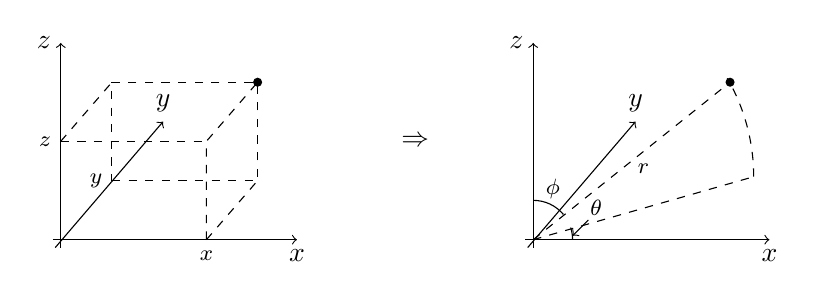
\begin{tikzpicture}
        \draw[->] (-0.1,0) -- (3,0) node[below] {$x$};
        \draw[->] (0,-0.1) -- (0,2.5) node[left] {$z$};
        \draw[->] (-0.07,-0.1) -- (1.3,1.5) node[above] {$y$};
        \draw[fill = black] (2.5,2) circle[radius = 0.05];
        \begin{scope}[style = dashed]
            \draw (0.65,0.75) -- (2.5,0.75) -- (2.5,2) -- (0.65,2) -- cycle;
            \draw (2.5-0.65,0) -- (2.5,0.75);
            \draw (2.5-0.65,0) -- (2.5-0.65,1.25) -- (2.5,2);
            \draw (0,1.25) -- (2.5-0.65,1.25);
            \draw (0,1.25) -- (0.65,2);
        \end{scope}
        \begin{scope}[every node/.append style = {font = \footnotesize}]
            \node at (2.5-0.65,-0.2) {$x$};
            \node at (-0.2,1.25) {$z$};
            \node at (0.65-0.2,0.75) {$y$};
        \end{scope}
        \node[every node/.append style = {font = \normalsize}] at (4.5,1.25) {$\Rightarrow$};
        \draw[->] (5.9,0) -- (9,0) node[below] {$x$};
        \draw[->] (6,-0.1) -- (6,2.5) node[left] {$z$};
        \draw[->] (6-0.07,-0.1) -- (7.3,1.5) node[above] {$y$};
        \draw[fill = black] (8.5,2) circle[radius = 0.05];
        \begin{scope}[style = dashed]
            \draw (6,0) -- (8.8,0.8);
            \draw (6,0) -- (8.5,2);
            \draw (8.8,0.8) arc (0:30:2.5);
        \end{scope}
        \draw (6.5,0) arc (0:18:0.5);
        \draw[rotate around = {40:(6,0)}] (6.5,0) arc (0:50:0.5);
        \begin{scope}[every node/.append style = {font = \footnotesize}]
            \node at (6.25,0.65) {$\phi$};
            \node at (7.4,0.9) {$r$};
            \node at (6.8,0.4) {$\theta$};
        \end{scope}
        \draw[<-] (6.5,0.05) -- (6.7,0.25);
    \end{tikzpicture}
    \caption{기본적인 직교좌표계에서 극좌표계(위), 원통좌표계(중간), 구면좌표계(아래)로의 변환.}
\end{figure}

\begin{corollary}
    음이 아닌 가측함수 $f:\mathbb{R}^2\to\overline{\mathbb{R}}^+_0,\,g:\mathbb{R}^3\to\overline{\mathbb{R}}^+_0$에 대해 다음이 성립한다.
    \begin{enumerate}
        \item (극좌표계 변환)
        \begin{equation*}
            \int_{\mathbb{R}^2}f(x,\,y)\,d\lambda_2(x,\,y)=\int_{\mathbb{R}^+_0\times[0,\,2\pi)}f(r\cos\theta,\,r\sin\theta)r\,d\lambda_2(r,\,\theta)
        \end{equation*}
        \item (원통좌표계 변환)
        \begin{equation*}
            \int_{\mathbb{R}^3}g(x,\,y,\,z)\,d\lambda_3(x,\,y,\,z)=\int_{\mathbb{R}^+_0\times[0,\,2\pi)\times\mathbb{R}}g(r\cos\theta,\,r\sin\theta,\,h)r\,d\lambda_3(r,\,\theta,\,h)
        \end{equation*}
        \item (구면좌표계 변환)
        \begin{align*}
            \int_{\mathbb{R}^3}&g(x,\,y,\,z)\,d\lambda_3(x,\,y,\,z)\\
            &=\int_{\mathbb{R}^+_0\times[0,\,\pi]\times[0,\,2\pi)}g(r\sin\theta\cos\phi,\,r\sin\theta\sin\phi,\,r\cos\theta)r^2\sin\theta\,d\lambda_3(r,\,\theta,\,\phi)
        \end{align*}
    \end{enumerate}
    한편, 적분가능한 $f:\mathbb{R}^2\to\overline{\mathbb{R}},\,g:\mathbb{R}^3\to\overline{\mathbb{R}}$에 대해서도 동일한 결과가 성립한다.
\end{corollary}

\begin{proof}
    함수
    \begin{align*}
        &\Phi_1:\mathbb{R}^+\times(0,\,2\pi)\to\mathbb{R}^2\setminus(\mathbb{R}^+_0\times\{0\})\\
        &\Phi_2:\mathbb{R}^+\times(0,\,2\pi)\times\mathbb{R}\to\mathbb{R}^3\setminus(\mathbb{R}^+_0\times\{0\}\times\mathbb{R})\\
        &\Phi_3:\mathbb{R}^+\times(0,\,\pi)\times(0,\,2\pi)\to\mathbb{R}^3\setminus(\mathbb{R}^+_0\times\{0\}\times\mathbb{R})
    \end{align*}
    을 각각
    \begin{align*}
        &\Phi_1:(r,\,\theta)\mapsto(r\cos\theta,\,r\sin\theta)\\
        &\Phi_2:(r,\,\theta,\,h)\mapsto(r\cos\theta,\,r\sin\theta,\,h)\\
        &\Phi_3:(r,\,\theta,\,\phi)\mapsto(r\sin\theta\cos\phi,\,r\sin\theta\sin\phi,\,r\cos\theta)
    \end{align*}
    로 정의하면 이들이 $\mathcal{C}^1$급 미분동형사상임을 쉽게 확인할 수 있고,
    \begin{align*}
        &\det\D\Phi_1(r,\,\theta)=\det
        \begin{bmatrix*}
            \cos\theta&-r\sin\theta\\
            \sin\theta&r\cos\theta
        \end{bmatrix*}
        =r\\
        &\det\D\Phi_2(r,\,\theta,\,h)=\det
        \begin{bmatrix*}
            \cos\theta&-r\sin\theta&0\\
            \sin\theta&r\cos\theta&0\\
            0&0&1
        \end{bmatrix*}
        =r\\
        &\det\D\Phi_3(r,\,\theta,\,\phi)=\det
        \begin{bmatrix*}
            \sin\theta\cos\phi&r\cos\theta\cos\phi&-r\sin\theta\sin\phi\\
            \sin\theta\sin\phi&r\cos\theta\sin\phi&r\sin\theta\cos\phi\\
            \cos\theta&-r\sin\theta&0
        \end{bmatrix*}
        =r^2\sin\theta
    \end{align*}
    이므로 변수변환 공식과 보조정리 \ref{lem:ReimannIntegrable}로부터 정리가 자명하다.
\end{proof}

다음은 변수변환 공식의 \texttt{Borel} 측도공간 버전이다.

\begin{corollary}
    열린집합 $U,\,V\subseteq\mathbb{R}^n$ 사이에서 정의된 $\mathcal{C}^1$급 전단사함수 $\Phi:U\to V$와 음이 아닌 \texttt{Borel} 함수 $f:\mathbb{R}^n\to\overline{\mathbb{R}}^+_0$에 대해 합성 $f\circ\Phi:U\to\overline{\mathbb{R}}^+_0$는 \texttt{Borel}이고 $\int_V f\,d\mu_n=\int_U(f\circ\Phi)|\det\D\Phi|\,d\mu_n$이다. 한편, $V$에서 $\mu_n$-적분가능한 (혹은 $(f\circ\Phi)|\det\D\Phi|$가 $U$에서 $\mu_n$-적분가능한) $f:\mathbb{R}^n\to\overline{\mathbb{R}}$에 대해서도 동일한 결과가 성립하며, 이때 $(f\circ\Phi)|\det\D\Phi|$는 $U$에서 $\mu_n$-적분가능하다 (혹은 $f$는 $V$에서 $\mu_n$-적분가능하다).
\end{corollary}

\begin{proof}
    이는 변수변환 공식과 정리 \ref{thm:compositionMeasurable}, \ref{thm:measureCompletionInt}로부터 자명하다.
\end{proof}

세 번째는 보조정리 \ref{lem:ReimannIntegrable}의 일반화로, 직관적으로도 꽤 자명하다.

\begin{corollary}\label{cor:subspaceNull}
    모든 부분공간 $\mathsf{V}<\mathbb{R}^n$는 영집합이다.
\end{corollary}

\begin{proof}
    영집합의 정의로부터 $\dim\mathsf{V}=n-1$인 경우만 생각하면 되고, 이때에 $\mathsf{V}$는 $\mathbb{R}^n$에서의 초평면이므로 만약 이가 $\mathbb{R}^n$의 좌표축 중 어느 하나와 직교한다면 보조정리 \ref{lem:ReimannIntegrable}로부터 정리가 자명하다. 만약 $\mathsf{V}$와 직교하는 좌표축이 존재하지 않는다면, 적당한 가역인 선형사상 $T:\mathbb{R}^n\to\mathbb{R}^n$가 존재하여 $T(\mathsf{V})$는 $\mathbb{R}^n$의 좌표축 중 어느 하나와 직교하는 초평면이고 $|\det T|=1$이므로\footnotemark 변수변환 공식과 앞선 결과로부터 $\lambda_n(T(\mathsf{V}))=\int_{\mathbb{R}^n}\ind_{T(\mathsf{V})}\,d\lambda_n=\int_{\mathbb{R}^n}(\ind_{T(\mathsf{V})}\circ T)|\det T|\,d\lambda_n=\int_{\mathbb{R}^n}\ind_{\mathsf{V}}\,d\lambda_n=\lambda_n(\mathsf{V})$에서 $\mathsf{V}$가 영집합임을 안다.
\end{proof}

마지막 따름정리는 선형사상의 행렬식과 측도로써 정의되는 넓이의 개념을 아름답게 연결해준다.

\begin{corollary}
    가측집합 $A\subseteq\mathbb{R}^n$와 선형사상 $T:\mathbb{R}^n\to\mathbb{R}^n$에 대해 $T(A)$도 가측이고, $\lambda_n(T(A))=|\det T|\lambda_n(A)$이다.
\end{corollary}

\begin{proof}
    만약 $T$가 가역이라면 변수변환 공식으로부터 $\lambda_n(A)=\int_{T(A)}|\det T^{-1}|\,d\lambda_n=\lambda_n(T(A))/|\det T|$가 되어 정리가 자명하다. 한편, $T$가 가역이 아니라면 $\mathrm{im}\,T<\mathbb{R}^n$이므로 따름정리 \ref{cor:subspaceNull}로부터 $\lambda_n(T(A))\leq\lambda_n(\mathrm{im}\,T)=0=|\det T|\lambda_n(A)$이다.
\end{proof}

\section{Fundamental Theorem of Calculus}

이번 절에서는 \texttt{FTC}로 돌아간다. \texttt{FTC}는 적분과 미분을 이어주는 다리 역할을 하는 정리로서 미적분학의 근간을 이루는 중요한 정리이다. 먼저, 우리가 1학년 미적분학 시간에 배운 기본적인 \texttt{FTC}를 보자.

\vspace{6pt}
\noindent{\ttfamily\bfseries Theorem (Fundamental theorem of calculus)} 다음이 성립한다.
\begin{enumerate}
    \item 적분가능한 연속함수 $f:\mathbb{R}\to\mathbb{R}$에 대해 함수 $F:\mathbb{R}\to\mathbb{R}$를 $F:x\mapsto\int_{-\infty}^xf\,d\lambda_1$로 두면 이는 $f$의 역도함수이다. 즉, $F'=f$이다.
    \item 함수 $F:\mathbb{R}\to\mathbb{R}$가 $\mathcal{C}^1$급이고 그 도함수가 적분가능하면 $f:=F'$에 대해 $F(x)=\int_{-\infty}^xf\,d\lambda_1$이다.
\end{enumerate}

쉽게 생각하면, i은 적분한 뒤 미분하면 원래의 함수를 얻는다는 의미이고, ii는 반대로 미분한 뒤 적분해도 원래의 함수를 얻는다는 의미로, 이 둘은 서로 필요충분과 비슷한 관계이다. 우리는 하도 많이 쓰는 까닭에 자명하게까지 느껴지는 이 \texttt{FTC}에 한 가지 간단하지만, 중요한 질문을 던진다. 만약 여기서 $f$가 연속이 아니면 어떻게 될까? 지금부터 우리는 이에 대해 답을 찾아나선다.

먼저 i을 보면, 함수 $F$를 정의할 수는 있어야 하므로 $f$가 적분가능하다는 조건은 필수적이다. 그러나 $f$가 적분가능하다는 조건만으로는 $F$의 미분가능성을 보장할 수가 없다. 실제로 적분가능하지만 $F$가 특정 점에서 미분불가능한 $f$를 쉽게 찾을 수 있다.\footnotemark 하지만 이렇게 허무하게 끝날 것이었으면 애초에 시작하지도 않았을 것이다. 놀랍게도, 비록 $F$가 모든 점에서 미분가능하지는 않지만, 이가 거의 대부분의 점에서 `미분 비슷한 무언가'를 할 수 있음을 보일 수 있다. 다만, 이를 증명하기 위해 준비해야 할 것들이 꽤나 많다. 먼저 비교적 간단한 적분가능한 함수의 근사부터 시작하자.

\begin{theorem}\label{thm:integrableApprox}
    적분가능한 $f:\mathbb{R}^n\to\overline{\mathbb{R}}$와 임의의 $\epsilon>0$에 대해 다음이 성립한다.
    \begin{enumerate}
        \item 단순함수 $g:\mathbb{R}^n\to\mathbb{R}$가 존재하여 이는 적당한 $a_1,\,\cdots,\,a_k\in\mathbb{R}$와 유계인 $B_1,\,\cdots,\,B_k\in\mathcal{S}_n$에 대해 $g=\sum_{i=1}^ka_i\ind_{B_i}$로 쓸 수 있으며 $\int_{\mathbb{R}^n}|f-g|\,d\lambda_n<\epsilon$이다.
        \item 적분가능한 연속함수 $g:\mathbb{R}^n\to\mathbb{R}$가 존재하여 $\int_{\mathbb{R}^n}|f-g|\,d\lambda_n<\epsilon$이다.
    \end{enumerate}
\end{theorem}

\begin{proof}
    i. 먼저 $f$가 음이 아닌 특별한 경우를 생각하면 정리 \ref{thm:measurableFunctionApprox}로부터 적당한 음이 아닌 단순함수 $f_i:\mathbb{R}^n\to\mathbb{R}^+_0$의 열 $\{f_i\}$가 존재하여 $f-f_i\downarrow0$이고 각 $i\in\mathbb{N}$에 대해 $f-f_i\leq f$이다. 그렇다면 \texttt{DCT}로부터 $\int_{\mathbb{R}^n}|f-f_i|\,d\lambda_n\to0$이고, 곧 임의의 $\epsilon>0$을 택하면 충분히 큰 $i_0\in\mathbb{N}$에 대해 $\int_{\mathbb{R}^n}|f-f_{i_0}|\,d\lambda_n<\epsilon/2$이다.

    표기의 편의를 위해 $\widetilde{f}:=f_{i_0}$로 두자. 함수 $\widetilde{f}$의 표준형을 $\sum_{j=1}^la_j\ind_{A_j}$라 하고, \texttt{WLOG}, 모든 $a_j$가 $0$이 아니라 하면 정리 \ref{thm:Complete2}, \ref{thm:LebesgueComplete}로부터 각 $j\leq l$에 대해 적당한 $B_j,\,C_j\in\mathcal{B}_n$가 존재하여 $B_j\subseteq A_j\subseteq C_j$이고 $C_j\setminus B_j$가 영집합이므로 $A_j\setminus B_j$도 영집합이다. 나아가, 집합족 $\mathcal{S}_n$이 $\mathcal{B}_n$의 생성자이고 각 $j\leq l$에 대해 $\mu_n(B_j)<\infty$임이 자명하므로(만약 어떤 $j_0\leq l$에 대해 $\mu_n(B_{j_0})=\infty$이면 $\lambda_n(A_{j_0})=\infty$이고, 곧 $\int_{\mathbb{R}^n}f\,d\lambda_n\geq\int_{\mathbb{R}^n}\widetilde{f}\,d\lambda_n=\sum_{j=1}^la_j\lambda_n(A_j)\geq a_{j_0}\lambda(A_{j_0})=\infty$가 되어 $f$가 적분가능하다는 가정에 모순된다.) 정리 \ref{thm:measureApprox}의 ii로부터 서로소인 $B_{j1},\,\cdots,\,B_{jm_j}\in\mathcal{S}_n$이 존재하여 $\mu_n(B_j\triangle\bigsqcup_{k=1}^{m_j}B_{jk})<\epsilon/2a_jl$이다. 이제 단순함수 $g=\sum_{j=1}^la_j\ind_{\bigsqcup_{k=1}^{m_j}B_{jk}}=\sum_{j=1}^l\sum_{k=1}^{m_j}a_j\ind_{B_{jk}},\,h=\sum_{j=1}^la_j\ind_{B_j}$를 생각하면 이상으로부터
    \begin{align*}
        \int_{\mathbb{R}^n}|g-h|\,d\lambda_n&=\int_{\mathbb{R}^n}\bigg|\sum_{j=1}^la_j(\ind_{\bigsqcup_{k=1}^{m_j}B_{jk}}-\ind_{B_j})\bigg|\,d\lambda_n\\
        &\leq\int_{\mathbb{R}^n}\sum_{j=1}^la_j\ind_{B_j\triangle\bigsqcup_{k=1}^{m_j}B_{jk}}\,d\lambda_n\\
        &=\sum_{j=1}^la_j\lambda_n\bigg(B_j\triangle\bigsqcup_{k=1}^{m_j}B_{jk}\bigg)\\
        &<\sum_{j=1}^l\frac{\epsilon}{2l}\\
        &=\frac{\epsilon}{2}
    \end{align*}
    이고 $\widetilde{f}=h$ (\texttt{ae.})이므로 따름정리 \ref{cor:zeroAeIntegral}의 ii로부터 $\int_{\mathbb{R}^n}|f-g|\,d\lambda_n\leq\int_{\mathbb{R}^n}|f-\widetilde{f}|\,d\lambda_n+\int_{\mathbb{R}^n}|\widetilde{f}-g|\,d\lambda_n<\epsilon/2+\int_{\mathbb{R}^n}|g-h|\,d\lambda_n<\epsilon$에서 정리가 성립한다.

    한편, 적분가능한 $f:\mathbb{R}^n\to\overline{\mathbb{R}}$에 대해서는 이를 양과 음의 부분으로 나누어 앞선 결과를 적용하면 된다.

    ii. 함수 $f$가 적분가능하므로 정리 \ref{thm:integralFinite}의 ii로부터 거의 어디서나 유한하고, \texttt{WLOG}, 필요하다면 영집합에서의 함숫값을 $0$으로 바꾸어 $f$가 항상 유한하다고 해도 된다. 그렇다면 i로부터 임의의 $\epsilon>0$을 택하면 단순함수 $h:\mathbb{R}^n\to\mathbb{R}$가 존재하여 이는 적당한 $a_1,\,\cdots,\,a_k\in\mathbb{R}$와 유계인 $B_1,\,\cdots,\,B_k\in\mathcal{S}_n$에 대해 $h=\sum_{i=1}^ka_i\ind_{B_i}$로 쓸 수 있으며 $\int_{\mathbb{R}^n}|f-h|\,d\lambda_n<\epsilon/2$이다. 이제 각 $i\leq k$와 임의의 $j\in\mathbb{N}$에 대해 $B_i$의 모서리를 조금씩 줄여 (단, 이때 $2/j$ 이상으로는 줄이지 않는 것으로 하자.) 만든 \texttt{semi-open box}를 $B_i'$라 하고 $B_i\setminus B_i'$에서 $h$의 함숫값인 $a_i$를 $0$과 선형으로 보간하여 얻는 함수를 $g_j:\mathbb{R}^n\to\mathbb{R}$라 하면 $|g_j-h|\to0$ (\texttt{ae.})이고(각 $i\leq k$에 대해 $j\to\infty$이면 $B_i'\uparrow B_i$이므로 함수열 $\{h_j\}$는 $\bigcup_{i=1}^k\partial B_i$를 제외한 모든 곳에서 $g$로 수렴한다. 그런데 주석 \ref{note:countableBoundaryNull}에서와 같은 이유로 $\lambda_n(\bigcup_{i=1}^k\partial B_i)=0$이므로 결국 $|g-h_j|\to0$ (\texttt{ae.})이다.) $|g_j-h|\leq|g_j|+|h|\leq2|h|$이므로 \texttt{DCT}에서 $\int_{\mathbb{R}^n}|g_j-h|\,d\lambda_n\to0$이다. 이는 곧 충분히 큰 $j_0\in\mathbb{N}$를 택하면 $\int_{\mathbb{R}^n}|g_{j_0}-h|\,d\lambda_n<\epsilon/2$임을 뜻하므로 $g:=g_{j_0}$라 하면 $\int_{\mathbb{R}^n}|f-g|\,d\lambda_n\leq\int_{\mathbb{R}^n}|f-h|\,d\lambda_n+\int_{\mathbb{R}^n}|g-h|\,d\lambda_n<\epsilon$이다. 이때 $g$가 연속임이 분명하고 $\int_X|g|\,d\lambda_n\leq\int_X|f-g|\,d\lambda_n+\int_X|f|\,d\lambda_n<\infty$에서 이가 적분가능하므로 정리가 성립한다.
\end{proof}

다음으로 필요한 것은 $\sigma$-대수와 측도의 \texttt{pushfowarding}이다. 이는 \texttt{pushfoward}라는 단어의 사전적 뜻 그대로 고정된 $\sigma$-대수나 측도에 대해 어떤 함수를 앞으로 `밀어넣어' 새로운 $\sigma$-대수나 측도를 얻는 방법이다. 엄밀한 정의를 보면 그 느낌을 더 잘 알 수 있을 것이다.

\begin{definition}
    측도공간 $(X,\,\mathcal{A},\,\mu)$와 집합 $Y$ 사이에서 정의된 함수 $\varphi:X\to Y$를 생각하자. 이때 $\varphi$에 대한 $\mathcal{A}$의 \textbf{\texttt{pushfoward} $\sigma$-대수(- $\sigma$-\texttt{algebra})}를 $\varphi_*\mathcal{A}$로 쓰고 $\varphi_*\mathcal{A}=\{A\subseteq Y:\varphi^{-1}(A)\in\mathcal{A}\}$로 정의한다. 비슷하게, $\varphi$에 대한 $\mu$의 \textbf{\texttt{pushfoward} 측도(- \texttt{measure})}를 $\varphi_*\mu:\varphi_*\mathcal{A}\to\overline{\mathbb{R}}^+_0$로 쓰고 $\varphi_*\mu:A\mapsto\mu(\varphi^{-1}(A))$로 정의한다.
\end{definition}

물론, 이때의 정의가 \texttt{well-define}되는지 확인해줘야 한다.

\begin{proposition}
    측도공간 $(X,\,\mathcal{A},\,\mu)$와 집합 $Y$ 사이에서 정의된 함수 $\varphi:X\to Y$에 대해 $(Y,\,\varphi_*\mathcal{A},\,\varphi_*\mu)$는 측도공간을 이룬다. 따라서 \texttt{pushfoward} $\sigma$-대수와 측도는 \texttt{well-define}된다.
\end{proposition}

\begin{proof}
    먼저 $\varphi_*\mathcal{A}$가 $\sigma$-대수임을 보이자. 이를 위해서는 정의 \ref{def:algebra}의 조건을 하나하나 따져보면 된다. 그 중 몇 개만 연습삼아 살펴보면, $\emptyset\in\mathcal{A}$에서 $\emptyset=\varphi^{-1}(\emptyset)\in\varphi_*\mathcal{A}$에서 $\varphi_*\mathcal{A}$가 비어있지 않음이 자명하다. 또한 임의의 $A\in\varphi_*\mathcal{A}$에 대해 $\varphi^{-1}(A)\in\mathcal{A}$이므로 $\varphi^{-1}(A^c)=[\varphi^{-1}(A)]^c\in\mathcal{A}$에서 $A^c\in\varphi_*\mathcal{A}$이다. 이제 남은 조건들도 이와 같이 쉽게 따져볼 수 있다.

    다음으로, $\varphi_*\mu$가 측도임을 보이자. 우선 $\varphi_*\mu(\emptyset)=\mu(\varphi^{-1}(\emptyset))=\mu(\emptyset)=0$임은 자명하고, $\varphi_*\mathcal{A}$에 속하는 임의의 서로소인 집합열 $\{A_i\}$에 대해 $\varphi_*\mu(\bigsqcup_{i=1}^\infty A_i)=\mu(\varphi^{-1}(\bigsqcup_{i=1}^\infty A_i))=\mu(\bigsqcup_{i=1}^\infty\varphi^{-1}(A_i))=\sum_{i=1}^\infty\mu(\varphi^{-1}(A_i))=\sum_{i=1}^\infty\varphi_*\mu(A_i)$이므로 $\varphi_*\mu$가 측도임을 알고, 증명이 끝난다.
\end{proof}

위의 정의에서 알 수 있듯이 \texttt{pushfowarding}은 $\varphi$에게 아무런 조건을 요구하지 않는다. 연속일 필요도, 전단사여야 할 필요도 없고, 심지어 가측일 필요도 없다. 앞서 배운 음이 아닌 가측함수의 적분으로 새로운 측도를 유도하는 것과 비교하면 \texttt{pushfowarding}은 보다 일반적인 상황에서도 적용할 수 있는 기법인 셈이다. 이러한 \texttt{pushfowarding}은 나중에 확률변수를 배우며 다시 등장할 것이다. 여기서는 \texttt{pushfowarding}에 대한 측도론적인 성질들을 조금 더 살펴보자.

\begin{theorem}
    가측공간 $(X,\,\mathcal{A})$와 집합 $Y$ 사이에서 정의된 함수 $\varphi:X\to Y$와 $Y$와 가측공간 $(Z,\,\mathcal{B})$ 사이에서 정의된 함수 $f:Y\to Z$에 대해 $f$가 $\varphi_*\mathcal{A}/\mathcal{B}$-가측일 필요충분조건은 $f\circ\varphi$가 $\mathcal{A}/\mathcal{B}$-가측인 것이다.
\end{theorem}

\begin{proof}
    충분조건임을 보이기 위해 임의의 $A\in\mathcal{B}$를 생각하면 가정으로부터 $f^{-1}(A)\in\varphi_*\mathcal{A}$이므로 $(f\circ\varphi)^{-1}(A)=\varphi^{-1}(f^{-1}(A))\in\mathcal{A}$에서 $f\circ\varphi$가 $\mathcal{A}/\mathcal{B}$-가측이 되어 충분조건임이 보여진다. 이제 필요조건임도 이와 비슷하게 보일 수 있다.
\end{proof}

\begin{theorem}[Transformation formula]
    측도공간 $(X,\,\mathcal{A},\,\mu)$와 집합 $Y$ 사이에서 정의된 함수 $\varphi:X\to Y$에 대해 음이 아닌 함수 $f:Y\to\overline{\mathbb{R}}^+_0$가 $\varphi_*\mathcal{A}/\mathcal{B}_1$-가측이라 하자. 그렇다면 합성 $f\circ\varphi:X\to\overline{\mathbb{R}}^+_0$는 가측이고 $\int_Yf\,d\varphi_*\mu=\int_Xf\circ\varphi\,d\mu$이다. 한편, $\varphi_*\mu$-적분가능한(혹은 $f\circ\varphi$가 $\mu$-적분가능한 가측함수) $f:Y\to\overline{\mathbb{R}}$에 대해서도 동일한 결과가 성립하며 이때 $f\circ\varphi$는 $\mu$-적분가능하다(혹은 $f$는 $\varphi_*\mu$-적분가능하다).
\end{theorem}

\begin{proof}
    먼저 $f$가 음이 아닌 단순함수인 경우를 생각하여 이의 표준형을 $f=\sum_{i=1}^ka_i\ind_{A_i}$라 하자. 그렇다면 $f\circ\varphi=\sum_{i=1}^ka_i\ind_{\varphi^{-1}(A_i)}$에서 이가 가측이고 $\int_Yf\,d\varphi_*\mu=\sum_{i=1}^ka_i\varphi_*\mu(A_i)=\sum_{i=1}^ka_i\mu(\varphi^{-1}(A_i))=\int_X\sum_{i=1}^ka_i\ind_{\varphi^{-1}(A_i)}\,d\mu=\int_Xf\circ\varphi\,d\mu$임이 분명하다. 이제 $f$를 음이 아닌 $\varphi_*\mathcal{A}/\mathcal{B}_1$-가측함수라 하면 정리 \ref{thm:measurableFunctionApprox}로부터 음이 아닌 단순함수 $f_i:Y\to\mathbb{R}^+_0$의 열 $\{f_i\}$가 존재하여 $f_i\uparrow f$이다. 여기서 각 $i\in\mathbb{N}$에 대해 $f_i\circ\varphi$가 가측이므로 정리 \ref{thm:limitMeasurable}의 ii에서 $f\circ\varphi$도 가측이고 \texttt{MCT}에서 $\int_Yf\,d\varphi_*\mu=\lim_{i\to\infty}\int_Yf_i\,d\varphi_*\mu=\lim_{i\to\infty}\int_Yf_i\circ\varphi\,d\mu=\int_Yf\circ\varphi\,d\mu$이다.


    한편, $\varphi_*\mu$-적분가능한 $f:Y\to\overline{\mathbb{R}}$에 대해서도 이를 양과 음의 부분으로 나누어 앞선 결과를 적용하면 $f\circ\varphi$가 $\mu$-적분가능하며 $\int_Yf\,d\varphi_*\mu=\int_Xf\circ\varphi\,d\mu$임을 쉽게 알 수 있고, $f\circ\varphi$가 $\mu$-적분가능한 가측함수 $f:Y\to\overline{\mathbb{R}}$에 대해서도 비슷하게 하면 된다.
\end{proof}

마지막 성질은 앞서 살펴본 변수변환 공식과 묘하게 닮은 부분이 있기에 두 정리 모두 변수변환 공식이라 불린다. 물론, 이러한 유사함은 기분탓만은 아니다. 더 파보면 분명 무언가 더 있겠지만 우리의 갈 길이 먼 까닭에 \texttt{pushfowarding}에 대해서는 이쯤으로 정리하자.\footnotemark

이번 절에서 \texttt{pushfowarding}이 필요한 이유는 바로 다음의 유명한 부등식 때문이다. 보통 확률론에서 쓰이는 이 부등식은 측도론에서도 유용하게 쓰이는 경우가 종종 있다. 나중에 확률론을 배우며 다른 부등식들도 만나볼 수 있을 것이다.

\begin{lemma}
    측도공간 $(X,\,\mathcal{A},\,\mu)$와 집합 $Y$ 사이에서 정의된 함수 $\varphi:X\to Y$와 집합 $A\in\varphi_*\mathcal{A}$에 대해 $\mu(\varphi^{-1}(A))=\int_X\ind_A\circ\varphi\,d\mu$이다.
\end{lemma}

\begin{proof}
    이는 $\int_X\ind_A\circ\varphi\,d\mu=\int_X\ind_A\,d\varphi_*\mu=\varphi_*\mu(A)=\mu(\varphi^{-1}(A))$로부터 자명하다.
\end{proof}

\begin{theorem}[Markov's inequality]
    측도공간 $(X,\,\mathcal{A},\,\mu)$에서 정의된 가측함수 $f:X\to\overline{\mathbb{R}}$와 임의의 $M,\,p>0$에 대해
    \begin{equation*}
        \mu\{|f(x)|\geq M\}\leq\frac{1}{M^p}\int_X|f|^p\,d\mu
    \end{equation*}
    가 성립한다.\footnotemark
\end{theorem}

\begin{proof}
    부등식 $\ind_{(-M,\,M)^c}\circ f=\ind_{(-1,\,1)^c}\circ(f/M)\leq(|f|/M)^p\ind_{(-1,\,1)^c}\circ(f/M)\leq(|f|/M)^p$와 위의 보조정리로부터 $\mu\{|f(x)|\geq M\}=\int_X\ind_{(-M,\,M)^c}\circ f\,d\mu\leq\int_X(|f|/M)^p\,d\mu$가 성립한다.
\end{proof}

이로써 준비는 끝났다. 이제 본격적으로 \texttt{FTC}의 i을 확장해보자. 먼저 `미분 비슷한 무언가'를 엄밀히 도입하기 위한 \texttt{framework}이 필요한데, 곧 증명할 \texttt{Hardy-Littlewood}의 정리가 그 역할을 해 줄 것이다.

\begin{definition}
    적분가능한 함수 $f:\mathbb{R}^n\to\overline{\mathbb{R}}$에 대해 이의 \textbf{(\texttt{Hardy-Littlewood}) \texttt{maximal function}}을 $Mf:\mathbb{R}^n\to\overline{\mathbb{R}}^+_0$로 쓰고
    \begin{equation*}
        Mf:x\mapsto\sup_{r>0}\frac{1}{\lambda_n(B(x,\,r))}\int_{B(x,\,r)}|f|\,d\lambda_n
    \end{equation*}
    로 정의한다.
\end{definition}

\begin{proposition}
    적분가능한 함수 $f:\mathbb{R}^n\to\overline{\mathbb{R}}$에 대해 이의 \texttt{maximal function} $Mf$는 가측이다.
\end{proposition}

\begin{proof}
    만약 $(Mf)(x)=0$인 $x\in\mathbb{R}^n$가 존재하면 이는 곧 임의의 $i\in\mathbb{N}$에 대해 $\int_{B(x,\,i)}|f|\,d\lambda_n=0$임을 뜻하여 정리 \ref{thm:monoSeriesIntegral}의 i로부터 $\int_{\mathbb{R}^n}|f|\,d\lambda_n=\lim_{i\to\infty}\int_{B(x,\,i)}|f|\,d\lambda_n=0$이고, 곧 정리 \ref{thm:zeroAeIntegral}의 ii로부터 $f=0$ (\texttt{ae.})이다. 그런데 이 경우에는 $Mf=0$이 되어 이가 명백히 가측이므로 $Mf>0$이라 가정하자.

    이제 임의의 $x>0$에 대해 $(Mf)^{-1}((x,\,\infty])$가 가측이면 $(Mf)^{-1}([-\infty,\,x])=[(Mf)^{-1}((x,\,\infty])]^c$에서 $(Mf)^{-1}([-\infty,\,x])$도 가측이므로 $(Mf)^{-1}((x,\,\infty])$가 가측임을 보이는 것으로 충분하다. 이를 위해 임의의 $x>0$를 고정하고 $(Mf)^{-1}((x,\,\infty])$가 열려있음을 보이자. 여기서 임의의 $y\in(Mf)^{-1}((x,\,\infty])$도 고정하면 적당한 $r>0$이 존재하여
    \begin{equation*}
        \frac{1}{\lambda_n(B(y,\,r))}\int_{B(y,\,r)}|f|\,d\lambda_n>x
    \end{equation*}
    이다. 한편, $r_i\downarrow r$인 임의의 $\{r_i\}$에 대해 정리 \ref{thm:monoSeriesMeasure}의 ii로부터 $\lambda_n(B(y,\,r_i))\downarrow\lambda_n(B(y,\,r))$이므로 $\lim_{s\downarrow r}\lambda_n(B(y,\,s))=\lambda_n(B(y,\,r))$이고, 곧
    \begin{equation*}
        \lim_{s\downarrow r}\frac{1}{\lambda_n(B(y,\,s))}\int_{B(y,\,r)}|f|\,d\lambda_n=\frac{1}{\lambda_n(B(y,\,r))}\int_{B(y,\,r)}|f|\,d\lambda_n>x
    \end{equation*}
    에서 적당한 $s>r$가 존재하여
    \begin{equation*}
        \frac{1}{\lambda_n(B(y,\,s))}\int_{B(y,\,r)}|f|\,d\lambda_n>x
    \end{equation*}
    이다. 또한, 임의의 $z\in B(y,\,s-r)$에 대해 $w\in B(y,\,r)$이면 $||z-w||\leq||z-y||+||y-w||<s$이므로 $B(y,\,r)\subseteq B(z,\,s)$이고, 곧 \texttt{Lebesgue} 측도의 이동 불변성으로부터
    \begin{align*}
        x&<\frac{1}{\lambda_n(B(y,\,s))}\int_{B(y,\,r)}|f|\,d\lambda_n\\
        &\leq\frac{1}{\lambda_n(B(y,\,s))}\int_{B(z,\,s)}|f|\,d\lambda_n\\
        &=\frac{1}{\lambda_n(B(z,\,s))}\int_{B(z,\,s)}|f|\,d\lambda_n\\
        &=(Mf)(z)
    \end{align*}
    가 되어 $z\in(Mf)^{-1}((x,\,\infty])$, 즉 $B(y,\,s-r)\subseteq(Mf)^{-1}((x,\,\infty])$에서 증명이 끝난다.
\end{proof}

\begin{lemma}[Vitali covering lemma]
    집합 $\mathbb{R}^n$에 속하는 열린 \texttt{ball}의 모임 $\mathcal{C}$에 대해 $\bigcup\mathcal{C}$가 유계라면 $\mathcal{C}$에서 가산개의 서로소인 열린 \texttt{ball} $B(x_1,\,r_1),\,B(x_2,\,r_2),\,\cdots$를 적당히 택하여 $\bigcup\mathcal{C}\subseteq\bigcup_{i=1}^kB(x_i,\,5r_i)$이도록 할 수 있다. (여기서 $k$는 유한할 수도, $\infty$일 수도 있다.)
\end{lemma}

\begin{proof}
    먼저 $d_1=\sup\{r\in\mathbb{R}^+_0:B(x,\,r)\in\mathcal{C}\}<\infty$에 대해 $r>d_1/2$인 열린 \texttt{ball} $B(x,\,r)\in\mathcal{C}$을 (가능하다면) 택하여 이를 $B(x_1,\,r_1)$이라 하자. 비슷하게 $d_2=\sup\{r\in\mathbb{R}^+_0:B(x,\,r)\in\mathcal{C},\,B(x,\,r)\cap B(x_1,\,r_1)=\emptyset\}<\infty$에 대해 $r>d_2/2$인 열린 \texttt{ball} $B(x,\,r)\in\mathcal{C}$을 (가능하다면) 택하여 이를 $B(x_2,\,r_2)$라 하고, 이를 가능할 때까지 반복하여 가산개의 열린 \texttt{ball} $B(x_1,\,r_1),\,B(x_2,\,r_2),\,\cdots$를 얻는다. 이제 이들이 모두 서로소임은 그 구성으로부터 자명하므로 $\bigcup\mathcal{C}\subseteq\bigcup_i^kB(x_i,\,5r_i)$만 보이면 된다. (여기서 $k$는 유한할 수도, $\infty$일 수도 있는데, 이제부터는 $k=\infty$라 생각하고 논의를 진행하도록 한다. $k$가 유한한 경우에도 비슷하게 하면 된다.)

    만약 어떤 $B(x,\,r)\in\mathcal{C}$가 존재하여 모든 $i\in\mathbb{N}$에 대해 $B(x,\,r)\cap B(x_i,\,r_i)=\emptyset$이라면 위의 구성으로부터 각 $i\in\mathbb{N}$에 대해 $r\leq d_i$이고, 곧 $r_i>d_i/2\geq r/2$에서 $\lambda_n(\bigsqcup_i^\infty B(x_i,\,r_i))=\sum_{i=1}^\infty\lambda_n(B(x_i,\,r_i))\geq\sum_{i=1}^\infty\lambda_n(B(x_i,\,r/2))=\infty$가 되어 $\bigcup\mathcal{C}$가 유계라는 가정에 모순되므로 임의의 $B(x,\,r)\in\mathcal{C}$에 대해 $B(x,\,r)\cap B(x_i,\,r_i)\ne\emptyset$인 $i\in\mathbb{N}$가 적어도 하나 존재한다. 이제 임의의 $B(x,\,r)\in\mathcal{C}$를 고정하고 $B(x,\,r)\cap B(x_i,\,r_i)\ne\emptyset$인 $i\in\mathbb{N}$ 중 가장 작은 것을 택하여 $i_0\in\mathbb{N}$라 하면 $B(x,\,r)\cap\bigsqcup_{i=1}^{i_0-1}B(x_i,\,r_i)=\emptyset$이고 곧 위의 구성으로부터 $r\leq d_{i_0}<2r_{i_0}$이다. 또한 $i_0$의 정의로부터 $B(x,\,r)\cap B(x_{i_0},\,r_{i_0})\ne\emptyset$이므로 임의의 $y\in B(x,\,r)$에 대해 $||x_{i_0}-y||\leq||x_{i_0}-x||+||x-y||<2r+r_{i_0}<5r_{i_0}$가 되어 $y\in B(x_{i_0},\,5r_{i_0})$, 즉 $B(x,\,r)\subseteq B(x_{i_0},\,5r_{i_0})$에서 $\bigcup\mathcal{C}\subseteq\bigcup_i^\infty B(x_i,\,5r_i)$임을 안다.
\end{proof}

\begin{lemma}
    적분가능한 함수 $f:\mathbb{R}^n\to\overline{\mathbb{R}}$와 임의의 $M>0$에 대해 $\lambda_n\{(Mf)(x)>M\}\leq5^n||f||_1/M$이다.
\end{lemma}

\begin{proof}
    임의의 $M>0$과 임의의 $i\in\mathbb{N}$를 고정하면 임의의 $x\in(Mf)^{-1}((M,\,\infty])\cap B(i)=:A_i$에 대해 적당한 $r_x>0$가 존재하여
    \begin{equation*}
        \frac{1}{\lambda_n(B(x,\,r_x))}\int_{B(x,\,r_x)}|f|\,d\lambda_n>M
    \end{equation*}
    에서 $\lambda_n(B(x,\,r_x))<\int_{B(x,\,r_x)}|f|/M\,d\lambda_n\leq||f||_1/M$이므로 $x\in A_i$의 선택과는 무관하게 적당한 $R>0$에 대해 $r_x\leq R$이고, 곧 $\bigcup_{x\in A_i}B(x,\,r_x)\subseteq\bigcup_{x\in A_i}B(x,\,R)\subseteq B(R+i)$에서 $\bigcup_{x\in A_i}B(x,\,r_x)$는 유계이다. 그렇다면 \texttt{Vitali covering lemma}로부터 $\{B(x,\,r_x)\}_{x\in A_i}$에 속하는 서로소인 열린 \texttt{ball}의 열 $\{B(x_j,\,r_{x_j})\}$가 존재하여 $\bigcup_{x\in A_i}B(x,\,r_x)\subseteq\bigcup_{j=1}^\infty B(x_j,\,5r_{x_j})$이다. 이로부터
    \begin{align*}
        \lambda_n(A_i)&\leq\lambda_n\bigg(\bigcup_{x\in A_i}B(x,\,r_x)\bigg)\\
        &\leq\lambda_n\bigg(\bigcup_{j=1}^\infty B(x_j,\,5r_{x_j})\bigg)\\
        &\leq\sum_{j=1}^\infty\lambda_n(B(x_j,\,5r_{x_j}))\\
        &=5^n\sum_{j=1}^\infty\lambda_n(B(x_j,\,r_{x_j}))\\
        &\leq\frac{5^n}{M}\sum_{j=1}^\infty\int_{B(x_j,\,r_{x_j})}|f|\,d\lambda_n\\
        &=\frac{5^n}{M}\int_{\bigsqcup_{j=1}^\infty B(x_j,\,r_{x_j})}|f|\,d\lambda_n\\
        &\leq\frac{5^n}{M}||f||_1
    \end{align*}
    이므로 정리 \ref{thm:monoSeriesMeasure}의 i에서 $\lambda_n\{(Mf)(x)>M\}=\lim_{i\to\infty}\lambda_n(A_i)\leq5^n||f||_1/M$이다.
\end{proof}

\begin{theorem}[Hardy-Littlewood]
    적분가능한 함수 $f:\mathbb{R}^n\to\overline{\mathbb{R}}$와 거의 대부분의 $x\in\mathbb{R}^n$에 대해 $r\downarrow0$이면
    \begin{equation*}
        \frac{1}{\lambda_n(B(x,\,r))}\int_{B(x,\,r)}|f-f(x)|\,d\lambda_n\to0
    \end{equation*}
    이다.
\end{theorem}

\begin{proof}
    임의의 적분가능한 $f:\mathbb{R}^n\to\overline{\mathbb{R}}$에 대해 함수 $f^*:\mathbb{R}^n\to\overline{\mathbb{R}}^+_0$를
    \begin{equation*}
        f^*:x\mapsto\limsup_{r\downarrow0}\frac{1}{\lambda_n(B(x,\,r))}\int_{B(x,\,r)}|f-f(x)|\,d\lambda_n
    \end{equation*}
    로 정의하고 이의 성질을 살펴보는 것으로 증명을 시작한다. 함수 $f,\,g:\mathbb{R}^n\to\overline{\mathbb{R}}$를 임의의 적분가능한 함수라 하면
    \begin{align*}
        &\limsup_{r\downarrow0}\frac{1}{\lambda_n(B(x,\,r))}\int_{B(x,\,r)}|(f+g)-(f+g)(x)|\,d\lambda_n\\
        &\quad\leq\limsup_{r\downarrow0}\frac{1}{\lambda_n(B(x,\,r))}\bigg[\int_{B(x,\,r)}|f-f(x)|\,d\lambda_n+\int_{B(x,\,r)}|g-g(x)|\,d\lambda_n\bigg]\\
        &\quad\leq\limsup_{r\downarrow0}\frac{1}{\lambda_n(B(x,\,r))}\int_{B(x,\,r)}|f-f(x)|\,d\lambda_n+\limsup_{r\downarrow0}\frac{1}{\lambda_n(B(x,\,r))}\int_{B(x,\,r)}|g-g(x)|\,d\lambda_n
    \end{align*}
    에서 $(f+g)^*\leq f^*+g^*$이다. 나아가, 만약 $g$가 $x_0\in\mathbb{R}^n$에서 연속이라면 임의의 $\epsilon>0$에 대해 적당한 $\delta>0$가 존재하여 $||x-x_0||<\delta$이면 $|g(x)-g(x_0)|<\epsilon$이므로 $r<\delta$이면
    \begin{equation*}
        \frac{1}{\lambda_n(B(x_0,\,r))}\int_{B(x_0,\,r)}|g-g(x_0)|\,d\lambda_n\leq\epsilon
    \end{equation*}
    에서 $g^*(x_0)=0$이다. 따라서 $g$가 연속이면 $g^*=(-g)^*=0$이 되어 $(f-g)^*\leq f^*+(-g)^*=f^*\leq(f-g)^*+g^*=(f-g)^*$에서 $(f-g)^*=f^*$이다. 한편,
    \begin{align*}
        \frac{1}{\lambda_n(B(x,\,r))}\int_{B(x,\,r)}|f-f(x)|\,d\lambda_n&\leq\frac{1}{\lambda_n(B(x,\,r))}\int_{B(x,\,r)}|f|+|f(x)|\,d\lambda_n\\
        &=\frac{1}{\lambda_n(B(x,\,r))}\int_{B(x,\,r)}|f|\,d\lambda_n+|f(x)|\\
        &\leq (Mf)(x)+|f(x)|
    \end{align*}
    에서 $f^*\leq Mf+|f|$도 성립한다.
    
    이상의 성질들을 정리하면 다음과 같다. 
    \begin{enumerate}
        \item 만약 $x_0\in\mathbb{R}^n$에서 $g$가 연속이면 $g^*(x_0)=0$이다.
        \item 만약 $g$가 연속이면 $(f-g)^*=f^*$이다.
        \item $f^*\leq Mf+|f|$.
    \end{enumerate}
    이제 임의의 적분가능한 $f:\mathbb{R}^n\to\overline{\mathbb{R}}$를 고정하고 $f^*=0$ (\texttt{ae.})임을 보이자. 이를 위해 임의의 $\epsilon>0$과 임의의 $M>0$을 택하면 정리 \ref{thm:integrableApprox}의 ii로부터 적당한 적분가능한 연속함수 $g:\mathbb{R}^n\to\mathbb{R}$가 존재하여 $||f-g||_1<M\epsilon/2(5^n+1)$이다. 한편, $(f-g)^*\leq M(f-g)+|f-g|$에서 $(f-g)^*>M$이면 $M(f-g)>M/2$이거나 $|f-g|>M/2$이므로 $[(f-g)^*]^{-1}((M,\,\infty])\subseteq[M(f-g)]^{-1}((M/2,\,\infty])\cup(|f-g|)^{-1}((M/2,\,\infty])$이고, 위의 보조정리와 \texttt{Markov}의 부등식으로부터
    \begin{align*}
        \lambda_n\bigg\{(M(f-g))(x)\geq\frac{M}{2}&\texttt{ or }|(f-g)(x)|\geq\frac{M}{2}\bigg\}\\
        &\leq\lambda_n\bigg\{(M(f-g))(x)\geq\frac{M}{2}\bigg\}+\lambda_n\bigg\{|f-g|(x)\geq\frac{M}{2}\bigg\}\\
        &\leq\frac{2\cdot5^n}{M}||f-g||_1+\frac{2}{M}||f-g||_1\\
        &<\epsilon
    \end{align*}
    이다. 이는 곧 $[M(f-g)]^{-1}((M/2,\,\infty])\cup(|f-g|)^{-1}((M/2,\,\infty])$가 영집합임을 함의하므로 $[(f-g)^*]^{-1}((M,\,\infty])$도 영집합이고, $(f-g)^*=f^*$에서 $(f^*)^{-1}((M,\,\infty])$도 영집합이다. 이제 $M$이 임의의 양수임을 상기한다면 $\{x\in\mathbb{R}^n:f^*(x)\ne0\}=\bigcup_{i=1}^\infty(f^*)^{-1}((1/i,\,\infty])$에서 $f^*=0$ (\texttt{ae.})이고, 증명은 이로써 충분하다.
\end{proof}

\begin{definition}
    적분가능한 함수 $f:\mathbb{R}^n\to\overline{\mathbb{R}}$와 $x\in\mathbb{R}^n$에 대해 $r\downarrow0$일 때
    \begin{equation*}
        \frac{1}{\lambda_n(B(x,\,r))}\int_{B(x,\,r)}|f-f(x)|\,d\lambda_n\to 0
    \end{equation*}
    이면 이때의 $x\in\mathbb{R}^n$를 $f$의 \textbf{\texttt{Lebesgue} 점(- \texttt{point})}라 한다.
\end{definition}

\begin{corollary}\label{cor:differentiableLebesguePoint}
    적분가능한 함수 $f:\mathbb{R}^n\to\overline{\mathbb{R}}$에 대해 이가 $x\in\mathbb{R}^n$에서 연속이라 하면 $x$는 \texttt{Lebesgue} 점이다.
\end{corollary}

\begin{proof}
    이는 위의 정리의 증명에서 밝힌 $f^*$의 성질 i로부터 자명하다.
\end{proof}

\texttt{Hardy-Littlewood}의 정리는 적분가능한 함수에 대해 모든 \texttt{Lebesgue} 점을 모은 집합은 영집합임을 함의한다. 뭔가 우리가 원하는 결과가 얻어지는 듯한 느낌이 든다. 그러나 통상적인 미분과 \texttt{Hardy-Littlewood}의 정리를 자연스럽게 연결하기에는 아직 조금 부족하다.

\begin{definition}
    집합족 $\mathcal{P}(\mathbb{R}^n)$에 속하는 가측인 집합열 $\{A_i\}$와 점 $x\in\mathbb{R}^n$에 대해 만약 적당한 상수 $C>0$와 $0$으로 수렴하는 양의 수열 $\{r_i\}$가 존재하여 각 $i\in\mathbb{N}$에 대해 $A_i\subseteq B(x,\,r_i)$이고 $\lambda_n(B(x,\,r_i))\leq C\lambda_n(A_i)$이면 이때의 집합열 $\{A_i\}$가 $x$로 \textbf{\texttt{regular}하게 수렴한다(\texttt{converge regularly})}고 한다.
\end{definition}

\begin{theorem}
    적분가능한 함수 $f:\mathbb{R}^n\to\overline{\mathbb{R}}$와 이의 \texttt{Lebesgue} 점 $x\in\mathbb{R}^n$, 그리고 $x$로 \texttt{regular}하게 수렴하는 $\mathcal{P}(\mathbb{R}^n)$에 속하는 가측인 집합열 $\{A_i\}$에 대해
    \begin{equation*}
        \frac{1}{\lambda_n(A_i)}\int_{A_i}|f-f(x)|\,d\lambda_n\to0
    \end{equation*}
    이다.
\end{theorem}

\begin{proof}
    가정으로부터 적당한 $C>0$와 $0$으로 수렴하는 양의 수열 $\{r_i\}$가 존재하여 $A_i\subseteq B(x,\,r_i)$이고 $\lambda_n(B(x,\,r_i))\leq C\lambda_n(A_i)$이므로 임의의 $i\in\mathbb{N}$에 대해
    \begin{equation*}
        \frac{1}{\lambda_n(A_i)}\int_{A_i}|f-f(x)|\,d\lambda_n\leq\frac{C}{\lambda_n(B(x,\,r_i))}\int_{B(x,\,r_i)}|f-f(x)|\,d\lambda_n
    \end{equation*}
    이다. 그런데 \texttt{Hardy-Littlewood}의 정리로부터 위 식의 우변이 $i\to\infty$이면 $0$으로 수렴하므로 증명이 끝난다.
\end{proof}

\begin{corollary}\label{cor:regularConverge}
    적분가능한 함수 $f:\mathbb{R}^n\to\overline{\mathbb{R}}$와 이의 \texttt{Lebesgue} 점 $x\in\mathbb{R}^n$, 그리고 $x$로 \texttt{regular}하게 수렴하는 $\mathcal{P}(\mathbb{R}^n)$에 속하는 가측인 집합열 $\{A_i\}$에 대해
    \begin{equation*}
        \frac{1}{\lambda_n(A_i)}\int_{A_i}f\,d\lambda_n\to f(x)
    \end{equation*}
    이다.
\end{corollary}

\begin{proof}
    임의의 $i\in\mathbb{N}$에 대해 $|\int_{A_i}f\,d\lambda_n-f(x)\lambda_n(A_i)|=|\int_{A_i}f-f(x)\,d\lambda_n|\leq\int_{A_i}|f-f(x)|\,d\lambda_n$이므로 따름정리는 자명하다.
\end{proof}

마침내 다음 정리를 얻는다. 이는 일반적인 $n$차원에서 적분가능한 함수에 대한 정리이므로 우리가 원했던 결과보다 더 강력한 결과이다.

\begin{definition}
    열린집합 $U\subseteq\mathbb{R}^n$에서 정의된 함수 $f:U\to\mathbb{R}$와 한 점 $x\in U$에 대해 극한 $\lim_{h\downarrow0}\Delta_{[x-h\ind,\,x+h\ind]}f/(2h)^n$이 수렴하면 $f$는 $x$에서 \textbf{\texttt{symmetric differentiable}}하다고 하고, 이때의 극한값을 $f^{(s)}(x)$로 쓴다. 나아가, 만약 $f$가 모든 $x\in U$에서 \texttt{symmetric differentiable}하면, 이때의 $f$를 \textbf{\texttt{symmetric differentiable}}하다고 한다.
\end{definition}

\begin{corollary}\label{cor:FTC1}
    적분가능한 함수 $f:\mathbb{R}^n\to\overline{\mathbb{R}}$에 대해 함수 $F:\mathbb{R}^n\to\mathbb{R}$를
    \begin{equation*}
        F:x\mapsto\int_{(-\infty,\,x]}f\,d\lambda_n
    \end{equation*}
    로 두면 $F^{(s)}=f$ (\texttt{ae.})이다. 나아가, $x_0\in\mathbb{R}^n$의 근방에서 $\partial^\ind F$이 존재하고 이가 $x_0$에서 연속이면 $F^{(s)}(x_0)=\partial^\ind F(x_0)$이다. (단, 여기서 $F$가 $x\in\mathbb{R}$에서 \texttt{symmetric differentiable}하지 않은 경우 $F^{{s}}(x)=0$으로 생각한다.)
\end{corollary}

\begin{proof}
    간결한 논의를 위해 $n=2$인 경우만 생각하자. ($n=1$인 경우를 포함한 일반적인 경우에도 이와 비슷하게 보일 수 있다.) 이제 임의의 \texttt{Lebesgue} 점 $x\in\mathbb{R}^2$와 $0$으로 수렴하는 임의의 수열 $\{h_i\}$를 택하여 $B_x(h_i)=[x_1-h_i,\,x_1+h_i]\times[x_2-h_i,\,x_2+h_i]$라 하면 $\{B_x(h_i)\}$가 $x$로 \texttt{regular}하게 수렴함을 쉽게 보일 수 있다. 그렇다면 따름정리 \ref{cor:regularConverge}로부터
    \begin{align*}
        \frac{\Delta_{B_x(h_i)}F}{(2h_i)^2}&=\frac{1}{(2h_i)^2}\bigg[\bigg(\int_{(-\infty,\,x_1+h_i]\times(-\infty,\,x_2+h_i]}f\,d\lambda_2-\int_{(-\infty,\,x_1-h_i]\times(-\infty,\,x_2+h_i]}f\,d\lambda_2\bigg)\\
        &\qquad\qquad\qquad-\bigg(\int_{(-\infty,\,x_1+h_i]\times(-\infty,\,x_2-h_i]}f\,d\lambda_2-\int_{(-\infty,\,x_1-h_i]\times(-\infty,\,x_2-h_i]}f\,d\lambda_2\bigg)\bigg]\\
        &=\frac{1}{(2h_i)^2}\int_{[x_1-h_i,\,x_1+h_i]\times[x_2-h_i,\,x_2+h_i]}f\,d\lambda_2\\
        &=\frac{1}{\lambda_2(B_x(h_i))}\int_{B_x(h_i)}f\,d\lambda_2\\
        &\to f(x)
    \end{align*}
    이므로 $F^{(s)}(x)=f(x)$이고, \texttt{Hardy-Littlewood}의 정리로부터 $\mathbb{R}^n$의 거의 대부분의 점들이 이러한 \texttt{Lebesgue} 점이므로 $F^{(s)}=f$ (\texttt{ae.})임을 안다.

    한편, $x_0\in\mathbb{R}^n$의 근방에서 $\partial^\ind F$가 존재하고 이가 $x_0$에서 연속이라 하자. 또한, 편의를 위해 편미분이 $\partial x_1\partial x_2$의 순서로 주어진 경우만 생각하자. (다른 경우에 대해서도 이와 비슷하게 보일 수 있다.) 그렇다면 따름정리 \ref{cor:differentiableLebesguePoint}에서 $x_0$는 \texttt{Lebesgue} 점이므로 앞선 결과로부터 $F$가 $x_0$에서 \texttt{symmetric differentiable}하고, \texttt{MVT}와 \texttt{L'H\^ospital}의 법칙으로부터
    \begin{align*}
        \lim_{h\downarrow0}&\frac{\Delta_{[x_0^1-h,\,x_0^1+h]\times[x_0^2-h,\,x_0^2+h]}F}{(2h)^2}\\
        &=\lim_{h\downarrow0}\frac{1}{2h}\bigg[\frac{F(x_0^1+h,\,x_0^2+h)-F(x_0^1+h,\,x_0^2-h)}{2h}-\frac{F(x_0^1-h,\,x_0^2+h)-F(x_0^1-h,\,x_0^2-h)}{2h}\bigg]\\
        &=\lim_{h\downarrow0}\frac{1}{2h}\bigg[\frac{\partial F(x_0^1+h,\,y_h)}{\partial x_2}-\frac{\partial F(x_0^1-h,\,z_h)}{\partial x_2}\bigg]\\
        &=\lim_{h\downarrow0}\frac{1}{2}\bigg[\frac{\partial^2F(x_0^1+h,\,y_h)}{\partial x_1\partial x_2}-\frac{\partial^2F(x_0^1-h,\,z_h)}{\partial x_1\partial x_2}\bigg]\\
        &=\frac{\partial^2 F}{\partial x_1\partial x_2}(x_0)
    \end{align*}
    가 되어 증명이 끝난다. 여기서 $y_h,\,z_h$는 모두 $x_0^2-h$와 $x_0^2+h$를 잇는 선분 위에 존재하는 점들로 \texttt{MVT}에서 그 존재가 보장된다.
\end{proof}

비록 위의 정리에서는 $F$가 \texttt{symmetric differentiable}하지 않은 $x\in\mathbb{R}$에서의 $F^{(s)}(x)$의 값을 $0$이라는 \texttt{dummy value}로 두었지만, \texttt{Hardy-Littlewood}의 정리로부터 이런 점의 집합이 영집합을 이루므로 정리의 성립여부는 이때의 \texttt{dummy value}의 선택과는 무관하다. 이러한 사실은 뒤따르는 \texttt{FTC}의 일반화에 대해서도 마찬가지이다. 이제 위의 정리에서 $n=1$인 경우를 기존의 \texttt{FTC}의 i에 대입하면 다음을 얻는다.

\vspace{6pt}
\noindent{\ttfamily\bfseries Theorem (Fundamental theorem of calculus)} i. 적분가능한 함수 $f:\mathbb{R}\to\mathbb{R}$에 대해 함수 $F:\mathbb{R}\to\mathbb{R}$를 $F:x\mapsto\int_{-\infty}^xf\,d\lambda_1$로 두면 $F^{(s)}=f$ (\texttt{ae.})이다.

\vspace{6pt}
여기서의 극한은 꽤나 익숙하다. 고등학교 문제집에서 한 번쯤은 보았을 이 극한은 정말 `미분 비슷한 무언가'이지만 항상 미분과 그 값이 같은 것도 아니고, 이 극한의 존재성이 미분가능성을 함의하는 것도 아니다. 하지만, 이는 $f$의 연속성을 포기한 대가이므로 이 정도에 만족하도록 하자.

이제 기존의 \texttt{FTC}의 ii를 살펴보는 것으로 이번 절의 후반부를 시작한다. 앞서 i을 일반화시킨 것과 비슷하게, $F$가 $\mathcal{C}^1$급이라는 조건을 $F$가 거의 어디서나 \texttt{symmetric differentiable}하다는 조건으로 바꾸어보자. 아쉽게도 아직은 한참 부족하다. 생각해보면, 이는 굉장히 순진한 시도였다. 만약 $F$가 정말 $F(x)=\int_{-\infty}^xf\,d\lambda_1$을 만족한다면 이는 정리 \ref{thm:distributionProp}의 iv와 $F(x)=\int_{-\infty}^xf_+\,d\lambda_1-\int_{-\infty}^xf_-\,d\lambda_1=(\lambda_1)_{f_+}((-\infty,\,x])-(\lambda_1)_{f_-}((-\infty,\,x])$에서 반드시 오른쪽 연속인데, 우리는 $F$가 거의 어디서나 \texttt{symmetric differentiable}해야 할 것을 요구했을 뿐, 이의 연속성에 대해서는 생각하지 않았기 때문이다.

그렇다면 조금 더 머리를 써서 $F^{(s)}=f$ (\texttt{ae.})일 뿐만 아니라 $F$가 연속일 것까지 요구해보자. 그러나 아직도 부족하다. 즉, $F^{(s)}=f$ (\texttt{ae.})이고 $F$가 연속이지만 $F(x)\ne\int_{-\infty}^xf\,d\lambda_1$인 반례가 존재한다.\footnotemark 어쩌면 $f$의 연속성을 포기한 대가가 너무나도 커서 이를 대체할 좋은 조건이 없는 것은 아닐까? 다행히, 우리의 질문이 이렇게 재미없게 결론나지는 않는다. 지금 우리에게 필요한 적당한 조건은 바로 $F$의 절대연속성이다.

\begin{definition}
    함수 $f:\mathbb{R}^n\to\mathbb{R}$를 생각하자. 임의의 $\epsilon>0$에 대해 적당한 $\delta>0$가 존재하여 임의의 유계이고 서로소인 $B_1,\,\cdots,\,B_k\in\mathcal{S}_n$에 대해 $\sum_{i=1}^k\mu_n(B_i)<\delta$이면 $\sum_{i=1}^k|\Delta_{B_i}f|<\epsilon$을 만족하면 이때의 $f$를 \textbf{절대연속(\texttt{absolutely continuous})}이라 한다.
\end{definition}

이전 절에서 \texttt{Radon-Nikod\'ym} 도함수를 도입하며 측도의 절대연속을 정의했는데, 그 용어가 그대로 쓰이는 것은 단순한 우연의 일치가 아니다. 측도의 절대연속성과 함수의 절대연속성은 서로 긴밀히 연결되어 있다.

\begin{theorem}[Borel-Cantelli]
    측도공간 $(\mathbb{R}^n,\,\mathcal{B}_n,\,\mu)$에 속하는 임의의 집합열 $\{A_i\}$에 대해 $\sum_{i=1}^\infty\mu(A_i)<\infty$이면 $\mu(\limsup_{i\to\infty}A_i)=0$이다.
\end{theorem}

\begin{proof}
    임의의 $\epsilon>0$을 택하면 충분히 큰 $i_0\in\mathbb{N}$에 대해 $\sum_{i=i_0}^\infty\mu(A_i)<\epsilon$인데, 정의로부터 $\limsup_{i\to\infty}A_i\subseteq\bigcup_{i=i_0}^\infty A_i$이므로 $\mu(\limsup_{i\to\infty}A_i)\leq\mu(\bigcup_{i=i_0}^\infty A_i)\leq\sum_{i=i_0}^\infty\mu(A_i)<\epsilon$에서 $\mu(\limsup_{i\to\infty}A_i)=0$임을 안다.
\end{proof}

\begin{theorem}\label{thm:AbsContiRel}
    $\sigma$-유한 측도공간 $(\mathbb{R}^n,\,\mathcal{B}_n,\,\mu)$에 대해 함수 $F_\mu:\mathbb{R}^n\to\mathbb{R}^+_0$를 $F_\mu:x\mapsto\mu(\prod_{i=1}^n(-\infty,\,x_i])$로 두자. 그렇다면 $F_\mu$가 절대연속일 필요충분조건은 $\mu\ll\mu_n$인 것이다.
\end{theorem}

\begin{proof}
    충분조건임을 보이기 위해서는 $\mu_n(N)=0$인 임의의 $N\in\mathcal{B}_n$을 고정하고 $\mu(N)=0$임을 보이면 충분하다. 이제 임의의 $\epsilon>0$을 택하면 정리 \ref{thm:distributionProp}의 ii와 가정으로부터 임의의 $\delta>0$가 존재하여 임의의 유계이고 서로소인 $B_1,\,\cdots,\,B_k\in\mathcal{S}_n$에 대해 $\sum_{i=1}^k\mu_n(B_i)<\delta$이면 $\sum_{i=1}^k\mu(B_i)=\sum_{i=1}^k\Delta_{B_i}F_\mu<\epsilon$이다. 한편, 정리 \ref{thm:measureApprox}의 i과 \ref{thm:BorelGen2}로부터 $\mathcal{S}_n$에 속하는 적당한 서로소인 집합열 $\{B_i\}$가 존재하여 $N\subseteq\bigsqcup_{i=1}^\infty B_i$이고 $\sum_{i=1}^\infty\mu_n(B_i)=\mu_n(\bigsqcup_{i=1}^\infty B_i)-\mu_n(N)=\mu_n(\bigsqcup_{i=1}^\infty B_i\setminus N)<\delta$이다. 이상으로부터 임의의 $k\in\mathbb{N}$에 대해 $\sum_{i=1}^k\mu_n(B_i)<\delta$이므로 $\sum_{i=1}^k\mu(B_i)<\epsilon$이고, 곧 $\sum_{i=1}^\infty\mu(B_i)\leq\epsilon$이 되어 $\mu(N)\leq\mu(\bigsqcup_{i=1}^\infty B_i)=\sum_{i=1}^\infty\mu(B_i)\leq\epsilon$에서 $\mu(N)=0$임을 안다.

    다음으로, 필요조건임을 보이기 위해 $F_\mu$가 절대연속이 아니면 $\mu\ll\mu_n$이 아님을 보이자. 정리 \ref{thm:distributionProp}의 ii와 가정으로부터 적당한 $\epsilon>0$이 존재하여 임의의 $i\in\mathbb{N}$에 대해 유계이고 서로소인 $B_{i1},\,\cdots,\,B_{ik_i}\in\mathcal{S}_n$가 존재하여 $\mu_n(\bigsqcup_{j=1}^{k_i}B_{ij})=\sum_{j=1}^{k_i}\mu_n(B_{ij})<1/i^2$이고 $\mu(\bigsqcup_{j=1}^{k_i}B_{ij})=\sum_{j=1}^{k_i}\mu(B_{ij})=\sum_{j=1}^{k_i}\Delta_{B_{ij}}F_\mu\geq\epsilon$이다. 이로부터 집합열 $\{B_i\}$를 $B_i:=\bigsqcup_{j=1}^{k_i}B_{ij}$로 정의하면 $\sum_{i=1}^\infty\mu_n(B_i)=\sum_{i=1}^\infty\mu_n(\bigsqcup_{j=1}^{k_i}B_{ij})<\sum_{i=1}^\infty1/i^2<\infty$이므로 정리 \ref{thm:generalSeriesMeasure}와 \texttt{Borel-Cantelli}의 정리로부터 $\mu_n(\limsup_{i\to\infty}B_i)=0$이지만 $\mu(\limsup_{i\to\infty}B_i)\geq\limsup_{i\to\infty}\mu(B_i)=\limsup_{i\to\infty}\mu(\bigsqcup_{j=1}^{k_i}B_{ij})\geq\epsilon$이 되어 $\mu\ll\mu_n$이 아님을 안다.
\end{proof}

위의 정리는 놀라운 발견이라기보다 이러한 관계가 성립하도록 함수의 절대연속의 정의가 디자인되었다고 보는 것이 맞을 것 같다. (균등연속이나 \texttt{Lipschitz} 연속과 같은 다른 함수의 연속성의 정의에 비해 절대연속의 정의는 다소 복잡하고 기하학적 직관도 부족하다.) 아무튼 이로부터 우리가 원하던 결론을 얻을 수 있다.

\begin{theorem}\label{thm:FTC2}
    함수 $F:\mathbb{R}^n\to\mathbb{R}$가 다음을 만족한다고 하자.
    \begin{enumerate}
        \item 함수 $F$는 거의 어디서나 \texttt{symmetric differentiable}하다.
        \item 함수 $F$는 절대연속이고 오른쪽 연속이며 각 변수에 대해 증가한다.
        \item 유계인 \texttt{semi-open box} $B\subseteq\mathbb{R}^n$에 대해 $\Delta_BF\geq0$이다.
        \item 각 $i\leq n$에 대해 $\lim_{x_i\to-\infty}F(x)=0$이다.
        \item $\lim_{x_1,\,\cdots,\,x_n\to\infty}F(x)<\infty$.
    \end{enumerate}
    그렇다면 $f:=F^{(s)}$에 대해 $F=\int_{(-\infty,\,x]}f\,d\lambda_n$이다.(단, 여기서 $F$가 $x\in\mathbb{R}^n$에서 \texttt{symmetric differentiable}하지 않은 경우 $f(x)=0$으로 생각한다.)
\end{theorem}

\begin{proof}
    먼저 정리 \ref{thm:finiteBorelSpecify}로부터 $\mathcal{B}_n$ 위의 적당한 측도 $\mu$가 존재하여 $F(x)=\mu(\prod_{i=1}^n(-\infty,\,x_i])$이고, 조건 v와 정리 \ref{thm:distributionProp}의 vii로부터 이때의 $\mu$는 유한하다. 그렇다면 조건 ii와 정리 \ref{thm:AbsContiRel}로부터 $\mu\ll\mu_n$이 되어 \texttt{Radon-Nikod\'ym} 도함수 $g:=d\mu/d\mu_n$가 존재하고 정리 \ref{thm:measureCompletionInt}로부터 $F(x)=\mu(\prod_{i=1}^n(-\infty,\,x_i])=\int_{\prod_{i=1}^n(-\infty,\,x_i]}g\,d\mu_n=\int_{\prod_{i=1}^n(-\infty,\,x_i]}g\,d\lambda_n$이다. 그런데 우리가 앞서 일반화한 \texttt{FTC} i로부터 $h\downarrow0$이면 $\lim_{h\downarrow0}\Delta_{B_x(h)}F/(2h)^n\to g(x)$ (\texttt{ae.})이므로 $f=g$ (\texttt{ae.})가 되어 정리 \ref{cor:zeroAeIntegral}의 ii로부터 $F=\int_{\prod_{i=1}^n(-\infty,\,x_i]}f\,d\lambda_n$이다.
\end{proof}

위의 정리에서 $n=1$인 경우를 기존의 \texttt{FTC}에 대입하면 다음을 얻는다.

\begin{proposition}
    절대연속함수 $f:\mathbb{R}\to\mathbb{R}$는 균등연속이다.
\end{proposition}

\begin{proof}
    거의 자명하다. 함수 $f$가 절대연속이므로 임의의 $\epsilon>0$에 대해 적당한 $\delta>0$가 존재하여 임의의 유계인 반열린구간 $I=(x,\,y)\subseteq\mathbb{R}$에 대해 $|x-y|=\mu_1(I)<\delta$이면 $|f(x)-f(y)|=|\Delta_If|<\epsilon$이고, 이로부터 $f$가 균등연속임이 분명하다.
\end{proof}

\noindent{\ttfamily\bfseries Theorem (Fundamental theorem of calculus)} ii. 함수 $F:\mathbb{R}\to\mathbb{R}$가 다음을 만족한다고 하자.
\begin{enumerate}
    \item[a.] 함수 $F$는 거의 어디서나 \texttt{symmetric differentiable}하다.
    \item[b.] 함수 $F$는 절대연속인 증가함수이다.
    \item[c.] $\lim_{x\to-\infty}F(x)=0$.
    \item[d.] $\lim_{x\to\infty}F(x)<\infty$.
\end{enumerate}
그렇다면 $f:=F^{(s)}$에 대해 $F=\int_{-\infty}^xf\,d\lambda_1$이다.(단, 여기서 $F$가 $x\in\mathbb{R}$에서 \texttt{symmetric differentiable}하지 않은 경우 $f(x)=0$으로 생각한다.)

\vspace{6pt}
정리 \ref{thm:FTC2}에서의 조건들이 $n=1$인 경우에는 많이 간단해진 것을 볼 수 있다. 그렇지만 뭔가 만족스럽지 못한 것도 사실이다. 일반적인 $n\in\mathbb{N}$에 대해 절대연속이라는 개념이 그 이름이 무색하게 오른쪽 연속성조차 함의하지 못하고, \texttt{FTC}의 ii의 확장이라고는 했지만 $F$에는 여전히 많은 조건들이 붙어있다. 특히 $F$가 증가함수인 경우로 한정된 것은 누가 보더라도 불필요하게 강하게 주어진 감이 있다. 하지만 나중에 필요한 정리나 개념은 모두 소개했고, 보다 나은 결과를 얻기 위해서는 지금까지의 논의와는 다른 별개의 논의가 필요한데, 이는 하나의 절에 담아내기에는 벅찬 내용이다. 이에 우리는 아쉬움을 뒤로 하고 여기서 멈추어 다음의 \texttt{FTC}를 얻은 것에 만족하기로 한다.\footnotemark

\begin{theorem}[Fundamental theorem of calculus]
    다음이 성립한다.
    \begin{enumerate}
        \item 적분가능한 함수 $f:\mathbb{R}\to\mathbb{R}$에 대해 함수 $F:\mathbb{R}\to\mathbb{R}$를 $F:x\mapsto\int_{-\infty}^xf\,d\lambda_1$로 두면 $F^{(s)}=f$ (\texttt{ae.})이다.
        \item 함수 $F:\mathbb{R}\to\mathbb{R}$가 다음을 만족한다고 하자.
        \begin{enumerate}
            \item[a.] 함수 $F$는 거의 어디서나 \texttt{symmetric differentiable}하다.
            \item[b.] 함수 $F$는 절대연속인 증가함수이다.
            \item[c.] $\lim_{x\to-\infty}F(x)=0$.
            \item[d.] $\lim_{x\to\infty}F(x)<\infty$.
        \end{enumerate}
        그렇다면 $f:=F^{(s)}$에 대해 $F=\int_{-\infty}^xf\,d\lambda_1$이다.(단, 여기서 $F$가 $x\in\mathbb{R}$에서 \texttt{symmetric differentiable}하지 않은 경우 $f(x)=0$으로 생각한다.)
    \end{enumerate}
\end{theorem}

\section{Convolution}

이번 절에서는 적분으로 정의되는 유명한 연산인 합성곱에 대한 엄밀한 이론 전개를 해 보기로 한다. 이미 대부분의 독자들이 알고 있겠지만 합성곱은 두 함수를 `곱하는' 특유의 방식으로 신호처리에서 두 신호를 합성하는 방법의 일종으로 널리 쓰인다. 우리도 이와 비슷하게 이후 확률론을 배우면서 두 확률변수를 더하는 과정에서 합성곱을 사용하게 될 것이다. 함수의 합성곱과 관련하여 필요한 이론의 전개가 이루어진 후에는 이와 유사하게 측도의 합성곱을 정의하고, 함수의 합성곱과 측도의 합성곱이 어떻게 연결되어 있는지를 살펴보도록 하자.

\begin{proposition}\label{prop:convolutionMeasurable}
    가측함수 $f:\mathbb{R}^n\to\overline{\mathbb{R}}$와 임의의 $x\in\mathbb{R}^n$에 대해 함수 $t\mapsto f(x-t)$는 가측이다.
\end{proposition}

\begin{proof}
    함수 $f_x:\mathbb{R}^n\to\mathbb{R}$와 미분동형사상 $\Phi_x:\mathbb{R}^n\to\mathbb{R}^n$를 각각 $f_x:t\mapsto f(x-t),\,\Phi_x:t\mapsto x-t$로 두면 변수변환 공식으로부터 $f_x=f\circ\Phi_x$가 가측이므로 이 명제는 자명하다.
\end{proof}

\begin{definition}
    가측함수 $f,\,g:\mathbb{R}^n\to\overline{\mathbb{R}}$에 대해 집합
    \begin{equation*}
        E(f,\,g)=\{x\in\mathbb{R}^n:\textrm{함수 $t\mapsto f(x-t)g(t)$가 적분가능하지 않다.}\}
    \end{equation*}
   를 생각하자. 이제 $f$와 $g$의 \textbf{합성곱(\texttt{convolution})}을 $f*g:\mathbb{R}^n\to\mathbb{R}$로 쓰고
    \begin{equation*}
        f*g:x\mapsto
        \begin{dcases*}
            \int_{\mathbb{R}^n}f(x-t)g(t)\,d\lambda_n(t)&$x\notin E(f,\,g)$인 경우\\
            0&\texttt{ow.}
        \end{dcases*}
    \end{equation*}
    로 정의한다.
\end{definition}

명제 \ref{prop:convolutionMeasurable}에서 함수 $t\mapsto f(x-t)g(t)$가 가측이므로 합성곱은 \texttt{well-define}되며 이로써 $f*g$를 아주 일반적으로 정의할 수 있다. 이제 합성곱의 기본적인 성질들을 알아보자.

\begin{theorem}\label{thm:aeConvolution}
    가측함수 $f,\,\widetilde{f},\,g,\,\widetilde{g}:\mathbb{R}^n\to\overline{\mathbb{R}}$에 대해 $f=\widetilde{f}$ (\texttt{ae.})이고 $g=\widetilde{g}$ (\texttt{ae.})이면 $E(f,\,g)=E(\widetilde{f},\,\widetilde{g})$이고 $f*g=\widetilde{f}*\widetilde{g}$이다.
\end{theorem}

\begin{proof}
    임의의 $x\in\mathbb{R}^n$에 대하여 함수 $f_x,\,\widetilde{f}_x:\mathbb{R}^n\to\mathbb{R}$와 미분동형사상 $\Phi_x:\mathbb{R}^n\to\mathbb{R}^n$를 각각 $f_x:t\mapsto f(x-t),\,\widetilde{f}_x:t\mapsto\widetilde{f}(x-t),\,\Phi_x:t\mapsto x-t$로 두면 명제 \ref{prop:convolutionMeasurable}로부터 $f_x$와 $\widetilde{f}_x$가 가측이다. 이제 집합 $M=\{x\in\mathbb{R}^n:f(x)\ne\widetilde{f}(x)\},\,N=\{x\in\mathbb{R}^n:g(x)\ne\widetilde{g}(x)\}$이 영집합이므로 임의의 $x\in\mathbb{R}^n$를 택하여 집합 $A_x=\{t\in\mathbb{R}^n:(f_xg)(t)\ne(\widetilde{f}_x\widetilde{g})(t)\}$를 생각하면 $A_x\subseteq\{t\in\mathbb{R}^n:x-t\in M\}\cup N=\Phi_x^{-1}(M)\cup N$이다. 그런데 $\Phi_x^{-1}$가 미분동형사상이고 곧 \texttt{Lipschitz} 연속이므로 보조정리 \ref{lem:LipschitzNull}로부터 $\Phi_x^{-1}(M)$이 영집합이 되어 $A_x$도 영집합이고, 이로부터 $f_xg=\widetilde{f}_x\widetilde{g}$ (\texttt{ae.})임을 안다. 이는 임의의 $x\in\mathbb{R}^n$에 대해 $f_xg$와 $\widetilde{f}_x\widetilde{g}$의 적분가능성이 일치함을 의미하므로 $E(f,\,g)=E(\widetilde{f},\,\widetilde{g})$가 성립하고, 이어서 $f*g=\widetilde{f}*\widetilde{g}$도 성립한다.
\end{proof}

\begin{theorem}\label{thm:convolutionBorel}
    가측함수 $f,\,g:\mathbb{R}^n\to\overline{\mathbb{R}}$에 대해 집합 $E(f,\,g)$는 \texttt{Borel}이고 함수 $f*g$도 \texttt{Borel}이다.
\end{theorem}

\begin{proof}
    정리 \ref{thm:LebesgueComplete}, \ref{thm:measureCompletionApprox}의 ii로부터 적당한 \texttt{Borel} 함수 $\widetilde{f},\,\widetilde{g}:\mathbb{R}^n\to\overline{\mathbb{R}}$가 존재하여 $f=\widetilde{f}$ (\texttt{ae.})이고 $g=\widetilde{g}$ (\texttt{ae.})이다. 이제 함수 $F:\mathbb{R}^{2n}\to\overline{\mathbb{R}}$를 $F:(x,\,t)\mapsto\widetilde{f}(x-t)\widetilde{g}(t)$로 두면 명제 \ref{prop:convolutionMeasurable}의 증명에서와 비슷하게 하여 이가 \texttt{Borel}임을 쉽게 보일 수 있다. 이로부터 함수 $G:\mathbb{R}^n\to\overline{\mathbb{R}}$를 $G:x\mapsto\int_{\mathbb{R}^n}|F(x,\,t)|\,d\mu(t)$로 정의하면 \texttt{Fubini}의 정리로부터 이는 \texttt{Borel}이고, 정리 \ref{thm:aeConvolution}로부터 $E(f,\,g)=E(\widetilde{f},\,\widetilde{g})=G^{-1}(\infty)=:E$도 \texttt{Borel}이다. 증명을 끝내기 위해 함수 $\widetilde{F}^\pm:\mathbb{R}^{2n}\to\overline{\mathbb{R}}$를
    \begin{equation*}
        \widetilde{F}^\pm:(x,\,t)\mapsto
        \begin{dcases*}
            F_\pm(x,\,t)&$x\notin E$\\
            0&\texttt{ow.}
        \end{dcases*}
    \end{equation*}
    로 두면 $\widetilde{F}^\pm$는 \texttt{Borel}이고, 다시 정리 \ref{thm:aeConvolution}로부터 임의의 $x\in\mathbb{R}^n$에 대해 $(f*g)(x)=(\widetilde{f}*\widetilde{g})(x)=\int_{\mathbb{R}^n}\widetilde{F}^+(x,\,t)\,d\mu(t)-\int_{\mathbb{R}^n}\widetilde{F}^-(x,\,t)\,d\mu(t)$이므로 \texttt{Fubini}의 정리로부터 $f*g$가 \texttt{Borel}임을 안다.
\end{proof}

이건 사실 조금 신기한 결과이다. 위의 정리에 따르면 비록 $f,\,g$ 각각은 가측인 함수에 그쳐 다루기 힘든 `이상한' 함수일 수 있지만, $f*g$는 \texttt{Borel}이 되어 그 합성곱은 반드시 `예쁜' 함수로 얻어진다. 이어서 살펴볼 것은 합성곱의 교환법칙과 분배법칙이다.

\begin{theorem}\label{thm:convolutionCommut}
    가측함수 $f,\,g:\mathbb{R}^n\to\overline{\mathbb{R}}$와 $c\ne0$에 대해 다음이 성립한다.
    \begin{enumerate}
        \item $E(f,\,g)=E(cf,\,g)=E(f,\,cg)$이고 $c(f*g)=(cf)*g=f*(cg)$이다.
        \item $E(f,\,g)=E(g,\,f)$이고 $f*g=g*f$이다.
    \end{enumerate}
\end{theorem}

\begin{proof}
    i. 우선 $E(f,\,g)=E(cf,\,g)=E(f,\,cg)=:E$임은 정의로부터 자명하고, 임의의 $x\in\mathbb{R}^n\setminus E$에 대해 $[c(f*g)](x)=c\int_{\mathbb{R}^n}f(x-t)g(t)\,d\lambda_n(t)=\int_{\mathbb{R}^n}cf(x-t)g(t)\,d\lambda_n(t)=[(cf)*g](x)$이므로 $c(f*g)=(cf)*g$이다. 이제 이와 비슷하게 $c(f*g)=f*(cg)$임도 보일 수 있다.

    ii. 임의의 $x\in\mathbb{R}^n$에 대하여 함수 $f_x,\,g_x:\mathbb{R}^n\to\overline{\mathbb{R}}$와 미분동형사상 $\Phi_x:\mathbb{R}^n\to\mathbb{R}^n$를 각각 $f_x:t\mapsto f(x-t),\,g_x:t\mapsto g(x-t),\,\Phi_x:t\mapsto x-t$로 정의하면 명제 \ref{prop:convolutionMeasurable}로부터 $f_x$와 $g_x$가 가측이다. 이제 임의의 $x\in\mathbb{R}^n$에 대해 $g_xf=(f_xg)\circ\Phi_x$이므로 변수변환 공식으로부터 $f_xg$와 $g_xf$의 적분가능성이 일치하여 $E(f,\,g)=E(g,\,f)=:E$이다. 나아가 임의의 $x\in\mathbb{R}^n\setminus E$에 대해 $(f*g)(x)=\int_{\mathbb{R}^n}f_xg\,d\lambda_n=\int_{\mathbb{R}^n}[(f_xg)\circ\Phi_x]|\det\D\Phi_x|\,d\lambda_n=\int_{\mathbb{R}^n}g_xf\,d\lambda_n=(g*f)(x)$이므로 $f*g=g*f$가 성립한다.
\end{proof}

\begin{theorem}\label{thm:convolutionDist}
    가측함수 $f,\,g,\,h:\mathbb{R}^n\to\overline{\mathbb{R}}$에 대해 $E(f,\,g+h)\subseteq E(f,\,g)\cup E(f,\,h)$이고 $\mathbb{R}^n\setminus[E(f,\,g)\cup E(f,\,h)]$에서 $f*(g+h)=f*g+f*h$이다. 단, 이때 $g+h$를 계산하는 과정에서 $\infty-\infty$와 같은 부정형이 등장하여 그 결과가 \texttt{well-define}되지 않는 경우 이를 $c\in\mathbb{R}$와 같은 \texttt{dummy-value}로 두는 관례를 전제하자.
\end{theorem}

\begin{proof}
    임의의 $x\in\mathbb{R}^n$에 대하여 함수 $f_x:\mathbb{R}^n\to\mathbb{R}$를 $f_x:t\mapsto f(x-t)$로 정의하면 명제 \ref{prop:convolutionMeasurable}로부터 $f_x$가 가측이다. 이제 $|f_x(g+h)|\leq|f_xg|+|f_xh|$이므로 정리 \ref{thm:integralFinite}의 i로부터 $E(f,\,g+h)\subseteq E(f,\,g)\cup E(f,\,h)=:E$임을 안다. 한편, 임의의 $x\in\mathbb{R}^n\setminus E$에 대해
    \begin{align*}
        [f*(g+h)](x)&=\int_{\mathbb{R}^n}f(x-t)(g+h)(t)\,d\lambda_n(t)\\
        &=\int_{\mathbb{R}^n}f(x-t)g(t)\,d\lambda_n(t)+\int_{\mathbb{R}^n}f(x-t)h(t)\,d\lambda_n(t)\\
        &=(f*g)(x)+(f*h)(x)
    \end{align*}
    이므로 $\mathbb{R}^n\setminus E$에서 $f*(g+h)=f*g+f*h$가 성립한다.
\end{proof}

다음으로, 합성곱의 결합법칙을 보자. 방금 살펴본 합성곱의 교환법칙과 분배법칙과는 달리, 결합법칙은 조금 복잡하다.

\begin{theorem}\label{thm:convolutionIneq}
    가측함수 $f,\,g:\mathbb{R}^n\to\overline{\mathbb{R}}$에 대해 $|f*g|\leq|f|*|g|$이다.
\end{theorem}

\begin{proof}
    임의의 $x\in\mathbb{R}^n$에 대해 만약 $x\in E(f,\,g)=E(|f|,\,|g|)$이면 $(f*g)(x)=(|f|*|g|)(x)=0$이 되어 정리가 자명하므로 $x\notin E(f,\,g)$라 하자. 그렇다면 $|(f*g)(x)|=|\int_{\mathbb{R}^n}f(x-t)g(t)\,d\lambda_n(t)|\leq\int_{\mathbb{R}^n}|f(x-t)g(t)|\,d\lambda_n(t)=(|f|*|g|)(x)$가 되어 증명이 끝난다.
\end{proof}

\begin{lemma}
    \texttt{Borel} 함수 $f,\,g,\,h:\mathbb{R}^n\to\overline{\mathbb{R}}$에 대해 $E(f,\,g),\,E(g,\,h)$가 영집합이면 $E(|f|,\,|g|*|h|)=E(|f|*|g|,\,|h|)$이다.
\end{lemma}

\begin{proof}
    임의의 $x\in\mathbb{R}^n$를 택하여 함수 $F_x:\mathbb{R}^{2n}\to\overline{\mathbb{R}}$를 각각 $F_x:(s,\,t)\mapsto f(x-t)g(t-s)h(s)$로 두면 명제 \ref{prop:convolutionMeasurable}의 증명에서와 비슷하게 하여 이가 \texttt{Borel}임을 쉽게 보일 수 있다. 그렇다면 $\int_{\mathbb{R}^n}|F_x(s,\,t)|\,d\lambda_n(s)=|f(x-t)|\int_{\mathbb{R}^n}|g(t-s)h(s)|\,d\lambda_n(s)=|f(x-t)|(|g|*|h|)(t)$가 임의의 $t\in\mathbb{R}^n\setminus E(|g|,\,|h|)$에 대해 성립하는데, 가정으로부터 $E:=E(|g|,\,|h|)=E(g,\,h)$가 영집합이므로 \texttt{Fubini}의 정리에서 
    \begin{align*}
        ||F_x||_1&=\int_{\mathbb{R}^n}\bigg[\int_{\mathbb{R}^n}|F_x(s,\,t)|\,d\lambda_n(s)\bigg]\,d\lambda_n(t)\\
        &=\int_{\mathbb{R}^n}|f(x-t)|\bigg[\int_{\mathbb{R}^n}|g(t-s)h(s)|\,d\lambda_n(s)\bigg]\,d\lambda_n(t)\\
        &=\int_{\mathbb{R}^n\setminus E}|f(x-t)|\bigg[\int_{\mathbb{R}^n}|g(t-s)h(s)|\,d\lambda_n(s)\bigg]\,d\lambda_n(t)\\
        &=\int_{\mathbb{R}^n\setminus E}|f(x-t)|(|g|*|h|)(t)\,d\lambda_n(t)\\
        &=\int_{\mathbb{R}^n}|f(x-t)|(|g|*|h|)(t)\,d\lambda_n(t)
    \end{align*}
    가 되어 $x\in E(|f|,\,|g|*|h|)$와 $||F_x||_1=\infty$가 서로 동치이다. 이와 비슷하게 $x\in E(|f|*|g|,\,|h|)$와 $||F_x||_1=\infty$가 서로 동치임도 보일 수 있으므로 $E(|f|,\,|g|*|h|)=E(|f|*|g|,\,|h|)$임을 안다.
\end{proof}

\begin{theorem}\label{thm:convolutionAsscoi}
    가측함수 $f,\,g,\,h:\mathbb{R}^n\to\overline{\mathbb{R}}$에 대해 $E(f,\,g),\,E(g,\,h)$가 영집합이면 $E:=E(|f|,\,|g|*|h|)=E(|f|*|g|,\,|h|)$이고 $\mathbb{R}^n\setminus E$에서 $f*(g*h)=(f*g)*h$이다.
\end{theorem}

\begin{proof}
    정리 \ref{thm:LebesgueComplete}, \ref{thm:measureCompletionApprox}의 ii로부터 적당한 \texttt{Borel} 함수 $\widetilde{f},\,\widetilde{g},\,\widetilde{h}:\mathbb{R}^n\to\overline{\mathbb{R}}$가 존재하여 $f=\widetilde{f}$ (\texttt{ae.}), $g=\widetilde{g}$ (\texttt{ae.}), $h=\widetilde{h}$ (\texttt{ae.})이고 정리 \ref{thm:aeConvolution}와 위의 보조정리로부터 $E(|f|,\,|g|*|h|)=E(|\widetilde{f}|,\,|\widetilde{g}|*|\widetilde{h}|)=E(|\widetilde{f}|*|\widetilde{g}|,\,|\widetilde{h}|)=E(|f|*|g|,\,|h|)$이다. 이제 임의의 $x\in\mathbb{R}^n\setminus E$를 택하여 함수 $F_x:\mathbb{R}^{2n}\to\overline{\mathbb{R}}$를 $F_x:(s,\,t)\mapsto\widetilde{f}(x-t)\widetilde{g}(t-s)\widetilde{h}(s)$로 두면 명제 \ref{prop:convolutionMeasurable}의 증명에서와 비슷하게 하여 이가 \texttt{Borel}임을 쉽게 보일 수 있다. 여기서 만약 $x\in E(\widetilde{f},\,\widetilde{g}*\widetilde{h})$이면 정리 \ref{thm:convolutionIneq}로부터 $\infty=\int_{\mathbb{R}^n}|\widetilde{f}(x-t)||(\widetilde{g}*\widetilde{h})(t)|\,d\lambda_n(t)\leq\int_{\mathbb{R}^n}|\widetilde{f}(x-t)|(|\widetilde{g}|*|\widetilde{h}|)(t)\,d\lambda_n(t)<\infty$의 모순이 발생하므로 $x\notin E(\widetilde{f},\,\widetilde{g}*\widetilde{h})$이고, 곧 \texttt{Fubini}의 정리, 정리 \ref{thm:aeConvolution}와 $E(g,\,h)=E(\widetilde{g},\,\widetilde{h})$가 영집합이라는 점으로부터
    \begin{align*}
        \int_{\mathbb{R}^{2n}}F_x\,d\lambda_{2n}&=\int_{\mathbb{R}^n}\bigg[\int_{\mathbb{R}^n}F_x(s,\,t)\,d\lambda_n(s)\bigg]\,d\lambda_n(t)\\
        &=\int_{\mathbb{R}^n}\widetilde{f}(x-t)\bigg[\int_{\mathbb{R}^n}\widetilde{g}(t-s)\widetilde{h}(s)\,d\lambda_n(s)\bigg]\,d\lambda_n(t)\\
        &=\int_{\mathbb{R}^n\setminus E(\widetilde{g},\,\widetilde{h})}\widetilde{f}(x-t)\bigg[\int_{\mathbb{R}^n}\widetilde{g}(t-s)\widetilde{h}(s)\,d\lambda_n(s)\bigg]\,d\lambda_n(t)\\
        &=\int_{\mathbb{R}^n\setminus E(\widetilde{g},\,\widetilde{h})}\widetilde{f}(x-t)(\widetilde{g}*\widetilde{h})(t)\,d\lambda_n(t)\\
        &=\int_{\mathbb{R}^n}\widetilde{f}(x-t)(\widetilde{g}*\widetilde{h})(t)\,d\lambda_n(t)\\
        &=[\widetilde{f}*(\widetilde{g}*\widetilde{h})](x)\\
        &=[f*(g*h)](x)
    \end{align*}
    이다. 한편, 비슷한 방법으로 $\int_{\mathbb{R}^{2n}}F_x\,d\lambda_{2n}=[(f*g)*h](x)$임을 보일 수 있으므로 $\mathbb{R}^n\setminus E$에서 $f*(g*h)=(f*g)*h$임을 안다.
\end{proof}

비록 앞서 얻은 분배법칙과 결합법칙은 훌륭한 결과이지만, 각각이 성립하기 위한 조건들 때문에 실용성이 떨어지는 것이 사실이다. 이러한 조건들을 생략하기 위해서는 합성곱을 취하는 함수들의 종류를 조금 제한할 필요가 있다. 즉, 지금까지는 임의의 두 가측함수에 합성곱을 취하는 것을 생각했다면, 이를 조금 제한하여 합성곱을 취해 보자는 것이다. 물론, 이때 너무 제한적으로 그 종류를 제한하면 또다시 실용성을 잃고 말겠지만, 다행히 다음 정리는 적당히 적분가능한 함수로 제한하는 것만으로 우리의 목적을 달성할 수 있음을 말해준다.

\begin{theorem}[Young's convolution inequality]
    임의의 $1/p+1/q=1+1/r$인 $p,\,q,\,r\geq1$과 임의의 $f\in L^p(\lambda_n),\,g\in L^q(\lambda_n)$에 대해 $E(f,\,g)$는 영집합이고 $||f*g||_r\leq||f||_p||q||_q$이다. 따라서 $f*g\in L^r$이다.
\end{theorem}

\begin{proof}
    함수 $h:\mathbb{R}^n\to\overline{\mathbb{R}}^+_0$를 $h:x\mapsto\int_{\mathbb{R}^n}|f(x-t)g(t)|\,d\lambda_n(t)$로 두면 이는 명제 \ref{prop:convolutionMeasurable}로부터 \texttt{well-define}되고 $E(f,\,g)=E(|f|,\,|g|)=h^{-1}(\infty)$이다. 한편, 정리 \ref{thm:convolutionIneq}로부터 $|f*g|\leq h$이므로 $||h||_r\leq||f||_p||g||_q$만 보일 수 있으면 $||f*g||_r\leq||f||_p||g||_q$는 자명해지고 $h\in L^r$이 되어 정리 \ref{thm:integralFinite}의 ii로부터 $h$가 거의 어디서나 유한하므로 증명이 끝난다. 이를 위해 임의의 $x\in\mathbb{R}^n$를 택하여 함수 $f_x:\mathbb{R}^n\to\overline{\mathbb{R}}$를 $f_x:t\mapsto f(x-t)$로 두고 $\lambda=p(1-1/q)$라 하면 명제 \ref{prop:convolutionMeasurable}로부터 $f_x$는 가측이고 $0\leq\lambda<1$이다. 먼저 $\lambda>0$인 경우를 생각하여 $s=p/\lambda$라 하면 $1/q+1/s=1$이므로 \texttt{H\"older}의 부등식으로부터 $h(x)=\int_{\mathbb{R}^n}|f_x|^\lambda|f_x|^{1-\lambda}|g|\,d\lambda_n\leq|||f_x|^{1-\lambda}|g|||_q|||f_x|^\lambda||_s$이고, 곧
    \begin{align*}
        [h(x)]^q&\leq\bigg[\int_{\mathbb{R}^n}|f_x|^{(1-\lambda)q}|g|^q\,d\lambda_n\bigg]\bigg(\int_{\mathbb{R}^n}|f_x|^{\lambda s}\,d\lambda_n\bigg)^{q/s}\\
        &=\bigg[\int_{\mathbb{R}^n}|f_x|^{(1-\lambda)q}|g|^q\,d\lambda_n\bigg]\bigg(\int_{\mathbb{R}^n}|f_x|^p\,d\lambda_n\bigg)^{\lambda q/p}\\
        &=\bigg[\int_{\mathbb{R}^n}|f_x|^{(1-\lambda)q}|g|^q\,d\lambda_n\bigg]||f_x||_p^{\lambda q}
    \end{align*}
    이며 이는 $\lambda=0$인 경우에도 성립함을 쉽게 알 수 있다. 그렇다면 $||f_x||_p=||f||_p$임은 자명하므로 \texttt{Minkowski}의 적분부등식으로부터 $s'=r/q$에 대해
    \begin{align*}
        ||h||_r^q&=\bigg(\int_{\mathbb{R}^n}h^r\,d\lambda_n\bigg)^{q/r}\\
        &=\bigg(\int_{\mathbb{R}^n}h^{qs'}\,d\lambda_n\bigg)^{1/s'}\\
        &\leq||f||_p^{\lambda q}\bigg\{\int_{\mathbb{R}^n}\bigg[\int_{\mathbb{R}^n}|f(x-t)|^{(1-\lambda)q}|g(t)|^q\,d\lambda_n(t)\bigg]^{s'}\,d\lambda_n(x)\bigg\}^{1/s'}\\
        &\leq||f||_p^{\lambda q}\int_{\mathbb{R}^n}\bigg[\int_{\mathbb{R}^n}|f(x-t)|^{(1-\lambda)qs'}|g(t)|^{qs'}\,d\lambda_n(x)\bigg]^{1/s'}\,d\lambda_n(t)\\
        &=||f||_p^{\lambda q}\int_{\mathbb{R}^n}\bigg[\int_{\mathbb{R}^n}|f(x)|^{(1-\lambda)qs'}\,d\lambda_n(x)\bigg]^{1/s'}|g(t)|^{q}\,d\lambda_n(t)\\
        &=||f||_p^{\lambda q}||f||_p^{(1-\lambda)q}||g||_q^q\\
        &=(||f||_p||g||_q)^q
    \end{align*}
    에서 $||h||_r\leq||f||_p||g||_q$임을 안다. 여기서 마지막에서 두 번째 등호는 $(1-\lambda)qs'=(1-\lambda)r=p$에서 성립한다.
\end{proof}

\begin{corollary}\label{cor:L1Convolution}
    적분가능한 $f,\,g:\mathbb{R}^n\to\overline{\mathbb{R}}$에 대해 $E(f,\,g)$는 영집합이고 $f*g$도 적분가능하다.
\end{corollary}

\begin{proof}
    이는 \texttt{Young}의 합성곱 부등식에서 $p=q=r=1$인 특별한 경우이다.
\end{proof}

따라서 $f,\,g$가 모두 적분가능한 경우에는 분배법칙과 결합법칙의 조건들을 생략하여 다음과 같이 간단히 쓸 수 있다. 이와 더불어 $L^1$ 공간은 합성곱 $*$에 대해 닫혀있다는 이상의 결론은 기억해둘만한 가치가 있다.

\begin{corollary}
    적분가능한 $f,\,g,\,h:\mathbb{R}^n\to\overline{\mathbb{R}}$와 $c\in\mathbb{R}$에 대해 다음이 성립한다.
    \begin{enumerate}
        \item (교환법칙) $c(f*g)=(cf)*g=f*(cg)$.
        \item (교환법칙) $f*g=g*f$.
        \item (결합법칙) $f*(g*h)=(f*g)*h$ (\texttt{ae.}).
        \item (분배법칙) $f*(g+h)=f*g+f*h$ (\texttt{ae.}).
    \end{enumerate}
\end{corollary}

\begin{proof}
    이는 정리 \ref{thm:convolutionCommut}, \ref{thm:convolutionDist}, \ref{thm:convolutionAsscoi}에 따름정리 \ref{cor:L1Convolution}를 적용한 결과로 자명하다.
\end{proof}

이제 측도의 합성곱을 정의하는 것으로 이번 절의 후반부를 시작한다.

\begin{proposition}\label{prop:convolutionMeasurable2}
    \texttt{Borel} 함수 $f:\mathbb{R}^n\to\overline{\mathbb{R}}$에 대해 함수 $F:\mathbb{R}^{2n}\to\overline{\mathbb{R}}$를 $F:(x,\,y)\mapsto f(x+y)$로 정의하면 이는 \texttt{Borel}이다.
\end{proposition}

\begin{proof}
    함수 $g:\mathbb{R}^{2n}\to\mathbb{R}^n$를 $g:(x,\,y)\mapsto x+y$로 두면 이가 연속이므로 곧 \texttt{Borel}이고, 정리 \ref{thm:compositionMeasurable}에서 $F=f\circ g$는 \texttt{Borel}이다.
\end{proof}

\begin{definition}
    \texttt{Borel} $\sigma$-대수 $\mathcal{B}_n$ 위의 측도 $\mu,\,\nu$에 대해 $\mu$와 $\nu$의 \textbf{합성곱(\texttt{convolution})}을 $\mu*\nu:\mathcal{B}_n\to\overline{\mathbb{R}}^+_0$로 쓰고 $\mu*\nu:A\mapsto\int_{\mathbb{R}^{2n}}\ind_A(x+y)\,d(\mu\otimes\nu)(x,\,y)$로 정의한다.
\end{definition}

\begin{proposition}
    \texttt{Borel} $\sigma$-대수 $\mathcal{B}_n$ 위의 측도 $\mu,\,\nu$에 대해 함수 $\mu*\nu$는 측도이다.
\end{proposition}

\begin{proof}
    우선 $(\mu*\nu)(\emptyset)=0$임은 분명하고, $\mathcal{B}_n$에 속하는 임의의 서로소인 집합열 $\{A_i\}$에 대해 \texttt{MCT}로부터
    \begin{align*}
        (\mu*\nu)\bigg(\bigsqcup_{i=1}^\infty A_i\bigg)&=\int_{\mathbb{R}^{2n}}\ind_{\bigsqcup_{i=1}^\infty A_i}(x+y)\,d(\mu\otimes\nu)(x,\,y)\\
        &=\int_{\mathbb{R}^{2n}}\sum_{i=1}^\infty\ind_{A_i}(x+y)\,d(\mu\otimes\nu)(x,\,y)\\
        &=\sum_{i=1}^\infty\int_{\mathbb{R}^{2n}}\ind_{A_i}(x+y)\,d(\mu\otimes\nu)(x,\,y)\\
        &=\sum_{i=1}^\infty(\mu*\nu)(A_i)
    \end{align*}
    이므로 $\mu*\nu$는 측도이다.
\end{proof}

명제 \ref{prop:convolutionMeasurable2}로부터 $\ind_A(x+y)$가 \texttt{Borel}이므로 측도의 합성곱은 \texttt{well-define}된다. 다음 순서는 측도의 합성곱의 기본적인 성질들을 살피는 것이다. 다행히 측도의 합성곱의 성질들은 함수의 합성곱의 성질들보다 쉽게 얻어진다.

\begin{theorem}\label{thm:convolutionInt}
    \texttt{Borel} $\sigma$-대수 $\mathcal{B}_n$ 위의 측도 $\mu,\,\nu,\,\xi$에 대해 $\xi=\mu*\nu$일 필요충분조건은 임의의 음이 아닌 \texttt{Borel} 함수 $f:\mathbb{R}^n\to\overline{\mathbb{R}}^+_0$에 대해 $\int_{\mathbb{R}^n}f\,d\xi=\int_{\mathbb{R}^{2n}}f(x+y)\,d(\mu\otimes\nu)(x,\,y)$인 것이다.
\end{theorem}

\begin{proof}
    충분조건임을 보이기 위해 먼저 $f$가 단순함수인 경우를 생각하여 이의 표준형을 $f=\sum_{i=1}^ka_i\ind_{A_i}$라 하면 $\int_{\mathbb{R}^n}f\,d\xi=\sum_{i=1}^ka_i\xi(A_i)=\sum_{i=1}^ka_i\int_{\mathbb{R}^{2n}}\ind_{A_i}(x+y)\,d(\mu\otimes\nu)(x,\,y)=\int_{\mathbb{R}^{2n}}f(x+y)\,d(\mu\otimes\nu)(x,\,y)$이다. 이제 일반적인 음이 아닌 \texttt{Borel} 함수 $f$를 생각하면 정리 \ref{thm:measurableFunctionApprox}로부터 적당한 단순함수 $f_i:\mathbb{R}^n\to\mathbb{R}^+_0$의 열 $\{f_i\}$가 존재하여 $f_i\uparrow f$이므로 \texttt{MCT}로부터 $\int_{\mathbb{R}^n}f\,d\xi=\lim_{i\to\infty}\int_{\mathbb{R}^n}f_i\,d\xi=\lim_{i\to\infty}\int_{\mathbb{R}^{2n}}f_i(x+y)\,d(\mu\otimes\nu)(x,\,y)=\int_{\mathbb{R}^{2n}}f(x+y)\,d(\mu\otimes\nu)(x,\,y)$가 되어 충분조건임이 보여진다.

    반대로, 필요조건임을 보이는 것은 쉽다. 임의의 $A\in\mathcal{B}_n$에 대해 $\ind_A$이 \texttt{Borel} 함수이므로 $\xi(A)=\int_{\mathbb{R}^n}\ind_A\,d\xi=\int_{\mathbb{R}^{2n}}\ind_A(x+y)\,d(\mu\otimes\nu)(x,\,y)=(\mu*\nu)(A)$에서 필요조건임이 분명하다.
\end{proof}

\begin{theorem}
    \texttt{Borel} $\sigma$-대수 $\mathcal{B}_n$ 위의 측도 $\mu,\,\nu,\,\xi$와 $c\geq0$에 대해 다음이 성립한다.
    \begin{enumerate}
        \item (교환법칙) $c(\mu*\nu)=(c\mu)*\nu=\mu*(c\nu)$.
        \item (교환법칙) $\mu*\nu=\nu*\mu$.
        \item (결합법칙) $\mu*(\nu*\xi)=(\mu*\nu)*\xi$.
        \item (분배법칙) $\mu*(\nu+\xi)=\mu*\nu+\mu*\xi$.
    \end{enumerate}
\end{theorem}

\begin{proof}
    임의의 $A\in\mathcal{B}_n$를 택하자.

    i. \texttt{Fubini}의 정리로부터
    \begin{align*}
        [c(\mu*\nu)](A)&=c\int_{\mathbb{R}^{2n}}\ind_A(x+y)\,d(\mu\otimes\nu)(x,\,y)\\
        &=c\int_{\mathbb{R}^n}\bigg[\int_{\mathbb{R}^n}\ind_A(x+y)\,d\mu(x)\bigg]\,d\nu(y)\\
        &=\int_{\mathbb{R}^n}\bigg[\int_{\mathbb{R}^n}\ind_A(x+y)\,d(c\mu)(x)\bigg]\,d\nu(y)\\
        &=\int_{\mathbb{R}^{2n}}\ind_A(x+y)\,d[(c\mu)\otimes\nu](x,\,y)\\
        &=[(c\mu)*\nu](A)
    \end{align*}
    에서 $c(\mu*\nu)=(c\mu)*\nu$이고 이와 비슷하게 $c(\mu*\nu)=\mu*(c\nu)$도 보일 수 있다.

    ii. \texttt{Fubini}의 정리로부터
    \begin{align*}
        (\mu*\nu)(A)&=\int_{\mathbb{R}^{2n}}\ind_A(x+y)\,d(\mu\otimes\nu)(x,\,y)\\
        &=\int_{\mathbb{R}^n}\bigg[\int_{\mathbb{R}^n}\ind_A(x+y)\,d\mu(x)\bigg]\,d\nu(y)\\
        &=\int_{\mathbb{R}^n}\bigg[\int_{\mathbb{R}^n}\ind_A(x+y)\,d\mu(y)\bigg]\,d\nu(x)\\
        &=\int_{\mathbb{R}^{2n}}\ind_A(x+y)\,d(\nu\otimes\mu)(x,\,y)\\
        &=(\nu*\mu)(A)
    \end{align*}
    에서 $\mu*\nu=\nu*\mu$이다.

    iii. \texttt{Fubini}의 정리와 정리 \ref{thm:convolutionInt}로부터
    \begin{align*}
        [\mu*(\nu*\xi)](A)&=\int_{\mathbb{R}^{2n}}\ind_A(x+y)\,d[\mu\otimes(\nu*\xi)](x,\,y)\\
        &=\int_{\mathbb{R}^n}\bigg[\int_{\mathbb{R}^n}\ind_A(x+y)\,d\mu(x)\bigg]\,d(\nu*\xi)(y)\\
        &=\int_{\mathbb{R}^{2n}}\bigg[\int_{\mathbb{R}^n}\ind_A(x+y+z)\,d\mu(x)\bigg]\,d(\nu\otimes\xi)(y,\,z)\\
        &=\int_{\mathbb{R}^n}\bigg\{\int_{\mathbb{R}^n}\bigg[\int_{\mathbb{R}^n}\ind_A(x+y+z)\,d\mu(x)\bigg]\,d\nu(y)\bigg\}\,d\xi(z)\\
        &=\int_{\mathbb{R}^n}\bigg[\int_{\mathbb{R}^{2n}}\ind_A(x+y+z)\,d(\mu\otimes\nu)(x,\,y)\bigg]\,d\xi(z)\\
        &=\int_{\mathbb{R}^n}\bigg[\int_{\mathbb{R}^n}\ind_A(x+z)\,d(\mu*\nu)(x)\bigg]\,d\xi(z)\\
        &=\int_{\mathbb{R}^{2n}}\ind_A(x+z)\,d[(\mu*\nu)\otimes\xi](x,\,z)\\
        &=[(\mu*\nu)*\xi](A)
    \end{align*}
    에서 $\mu*(\nu*\xi)=(\mu*\nu)*\xi$이다.

    iv. \texttt{Fubini}의 정리로부터
    \begin{align*}
        [\mu*(\nu+\xi)](A)&=\int_{\mathbb{R}^{2n}}\ind_A(x+y)\,d[\mu\otimes(\nu+\xi)](x,\,y)\\
        &=\int_{\mathbb{R}^n}\bigg[\int_{\mathbb{R}^n}\ind_A(x+y)\,d\mu(x)\bigg]\,d(\nu+\xi)(y)\\
        &=\int_{\mathbb{R}^n}\bigg[\int_{\mathbb{R}^n}\ind_A(x+y)\,d\mu(x)\bigg]\,d\nu(y)+\int_{\mathbb{R}^n}\bigg[\int_{\mathbb{R}^n}\ind_A(x+y)\,d\mu(x)\bigg]\,d\xi(y)\\
        &=\int_{\mathbb{R}^{2n}}\ind_A(x+y)\,d(\mu\otimes\nu)(x,\,y)+\int_{\mathbb{R}^{2n}}\ind_A(x+y)\,d(\mu\otimes\xi)(x,\,y)\\
        &=(\mu*\nu)(A)+(\mu*\xi)(A)
    \end{align*}
    에서 $\mu*(\nu+\xi)=\mu*\nu+\mu*\xi$이다.
\end{proof}

한편, 함수의 합성곱과 측도의 합성곱은 다음 정리에 의해 서로 연결되어 있다.

\begin{theorem}
    음이 아닌 적분가능한 \texttt{Borel} 함수 $f,\,g:\mathbb{R}^n\to\overline{\mathbb{R}}^+_0$에 대해 $(\mu_n)_f*(\mu_n)_g=(\mu_n)_{f*g}$이다.
\end{theorem}

\begin{proof}
    함수 $F:\mathbb{R}^{2n}\to\overline{\mathbb{R}}^+_0$를 $F:(x,\,y)\mapsto f(x-y)$로 두면 명제 \ref{prop:convolutionMeasurable2}의 증명에서와 비슷하게 하여 이가 \texttt{Borel}임을 쉽게 보일 수 있다. 이제 임의의 $A\in\mathcal{B}_n$를 택하면 \texttt{Fubini}의 정리로부터
    \begin{align*}
        [(\mu_n)_f*(\mu_n)_g](A)&=\int_{\mathbb{R}^{2n}}\ind_A(x+y)\,d[(\mu_n)_f\otimes(\mu_n)_g](x,\,y)\\
        &=\int_{\mathbb{R}^n}\bigg[\int_{\mathbb{R}^n}\ind_A(x+y)\,d(\mu_n)_f(x)\bigg]\,d(\mu_n)_g(y)\\
        &=\int_{\mathbb{R}^n}\bigg[\int_{\mathbb{R}^n}f(x)g(y)\ind_A(x+y)\,d\mu_n(x)\bigg]\,d\mu_n(y)\\
        &=\int_{\mathbb{R}^n}\bigg[\int_{\mathbb{R}^n}f(x-y)g(y)\ind_A(x)\,d\mu_n(x)\bigg]\,d\mu_n(y)\\
        &=\int_{\mathbb{R}^n}\bigg[\int_{\mathbb{R}^n}f(x-y)g(y)\ind_A(x)\,d\mu_n(y)\bigg]\,d\mu_n(x)
    \end{align*}
    인데, 정리 \ref{thm:convolutionBorel}와 따름정리 \ref{cor:L1Convolution}로부터 $E(f,\,g)$가 영집합이고 $f*g$도 음이 아닌 적분가능한 \texttt{Borel} 함수이므로 $[(\mu_n)_f*(\mu_n)_g](A)=\int_{\mathbb{R}^n}\ind_A(f*g)\,d\mu_n=\int_{\mathbb{R}^n}\ind_A\,d(\mu_n)_{f*g}=(\mu_n)_{f*g}(A)$이다.
\end{proof}

나중에 사용할 정리 하나를 증명하는 것으로 이번 절을 끝마치도록 하자.

\begin{theorem}
    \texttt{Borel} $\sigma$-대수 $\mathcal{B}_n$ 위의 측도 $\mu,\,\nu$와 임의의 $A\in\mathcal{B}_n$에 대해 함수 $x\mapsto\mu(A-x)$는 \texttt{Borel}이고 $(\mu*\nu)(A)=\int_{\mathbb{R}^n}\mu(A-x)\,d\nu(x)$이다.
\end{theorem}

\begin{proof}
    \texttt{Fubini}의 정리로부터
    \begin{align*}
        (\mu*\nu)(A)&=\int_{\mathbb{R}^{2n}}\ind_A(x+y)\,d(\mu\otimes\nu)(y,\,x)\\
        &=\int_{\mathbb{R}^n}\bigg[\int_{\mathbb{R}^n}\ind_A(x+y)\,d\mu(y)\bigg]\,d\nu(x)\\
        &=\int_{\mathbb{R}^n}\bigg[\int_{\mathbb{R}^n}\ind_{A-x}(y)\,d\mu(y)\bigg]\,d\nu(x)\\
        &=\int_{\mathbb{R}^n}\mu(A-x)\,d\nu(x)
    \end{align*}
    이고 이때 함수 $x\mapsto\mu(A-x)$가 \texttt{Borel}임이 분명하다.
\end{proof}

\section{Epilogue}

본 장의 마지막을 장식할 이번 절에서는 별개의 절로 구성할 정도의 내용은 아니지만, 그래도 놓치기는 아까운 주제들에 대해 가볍게 알아보도록 하겠다. 다루게 될 주제는 측도의 분해, 셈측도, 그리고 벡터함수와 복소함수의 적분으로 크게 3가지이다.

\subsection{Lebesgue's decomposition theorem}

우리는 주어진 임의의 측도를 보다 단순하거나 특정한 구조를 가지는 측도들의 합으로 분해할 수 있도록 해 주는 정리들을 통틀어 흔히 `분해정리'라 부른다. 이런 분해정리들은 다분히 이론적인 도구로, 마치 인수분해를 통해 정수의 성질을 더 깊이 탐구할 수 있는 것처럼 분해정리들로 측도를 적당히 분해함으로써 측도론의 깊이있는 이론을 전개할 수 있다. 이렇게 측도론에서 큰 의의를 가지는 정리들이지만 분해정리가 본격적으로 필요할 정도의 추상적인 측도론은 지나치다는 생각에 아쉽게도 이 책에서는 분해정리가 빛을 보지 못한 것이 사실이다. 그럼에도 불구하고, 이를 에필로그에서라도 뒤늦게 소개하는 까닭은 이가 확률론에서 그 자체로 나름 함의하는 바가 있고, 그 함의가 어쩌면 고등학교 때부터 궁금했을 수도 있는 `왜 이산확률변수와 연속확률변수에만 관심을 가지는가?'라는 질문에 대한 훌륭한 답변이 되기 때문이다. 그 답변은 확률의 현실적인 응용에서는 이산확률변수와 연속확률변수로 충분하다는 식의 공학도의 마인드가 물씬 풍기는 타협적인 답변보다 훨씬 지적으로 우아하고 만족스러울 것이다.

일단 이번 절은 에필로그인 만큼 그 답변을 듣는 것은 다음 장으로 잠시 미루어두고, 여기서는 분해정리를 증명하고, 내친 김에 이를 \texttt{Radon-Nikod\'ym} 도함수에 간단히 응용하는 정도로 만족하도록 하자. 우리는 \texttt{singular}라는 개념과 함께 앞서 미쳐 살펴보지 못했던 측도의 절대연속에 관한 성질을 살펴보는 것으로 논의를 시작한다.

\begin{definition}
    가측공간 $(X,\,\mathcal{A})$ 위의 측도 $\mu,\,\nu$에 대해 적당한 $A\in\mathcal{A}$가 존재하여 $\mu(A)=\nu(A^c)=0$이면 이때 $\mu$와 $\nu$는 서로 \textbf{\texttt{singular}}하다고 하고 $\mu\perp\nu$로 쓴다.
\end{definition}

측도 $\mu$와 $\nu$가 서로 singular하다는 것은, $\mu$와 $\nu$가 측도를 부여하는 데 있어 서로 공통된 정보를 사용하지 않는다는, 따라서 서로 독립적이라는 정도의 의미이다. 즉, 정의로부터 적당한 $A\in\mathcal{A}$가 존재하여 $\mu(A)=\nu(A^c)=0$인데, 임의의 $B\in\mathcal{A}$를 생각하면 $\mu(B)=\mu(B\cap A)+\mu(B\cap A^c)=\mu(B\cap A^c)$이고 $\nu(B)=\nu(B\cap A)+\nu(B\cap A^c)=\nu(B\cap A)$이므로 $\mu$는 $B\cap A^c$의 정보만으로 $B$에 측도를 부여하고, $\nu$는 $B\cap A$의 정보만으로 $B$에 측도를 부여하여 이 둘은 $B$의 측도를 부여하는 데 있어 서로 공통된 정보를 사용하지 않는다.

한편, 앞서 소개한 절대연속은 이와 정반대의 의미이다. 예컨대 $\mu\ll\nu$라 하고 적당한 $A\in\mathcal{A}$에 대해 $\nu(A^c)=0$이라 하면 $\nu$는 측도를 부여하는 데 있어 $A$에 속한 정보만을 사용한다고 생각할 수 있다. 그런데 정의로부터 $\mu(A^c)=0$이므로 $\mu$ 또한 $A$에 속한 정보만을 사용하고, $A$ 밖의 정보는 사용하지 못한다. 즉, $\mu$는 측도를 부여하는 데 있어 철저하게 $\nu$가 사용하는 정보만 사용할 수 있고, 곧 $\mu$는 $\nu$에 종속적이다.

\begin{proposition}\label{prop:singularMeasure}
    가측공간 $(X,\,\mathcal{A})$ 위의 측도 $\mu,\,\nu,\,\xi$에 대해 다음이 성립한다.
    \begin{enumerate}
        \item 만약 $\mu\perp\xi$이고 $\nu\perp\xi$이면 $(\mu+\nu)\perp\xi$이다.
        \item 만약 $\mu\ll\xi$이고 $\nu\ll\xi$이면 $(\mu+\nu)\ll\xi$이다.
        \item 만약 $\mu\ll\xi$이고 $\nu\perp\xi$이면 $\mu\perp\nu$이다.
        \item 만약 $\mu\ll\xi$이고 $\mu\perp\xi$이면 $\mu=0$이다. 
    \end{enumerate}
\end{proposition}

\begin{proof}
    i. 가정으로부터 적당한 $A,\,B\in\mathcal{A}$가 존재하여 $\mu(A)=\nu(B)=\xi(A^c)=\xi(B^c)=0$이므로 $\mu(A\cap B)\leq\mu(A)=0,\,\nu(A\cap B)\leq\nu(B)=0,\,\xi((A\cap B)^c)=\xi(A^c\cup B^c)\leq\xi(A^c)+\xi(B^c)=0$이고, 이로부터 $(\mu+\nu)\perp\xi$이다.

    ii. 가정으로부터 임의의 $N\in\mathcal{A}$에 대해 $\xi(N)=0$이면 $(\mu+\nu)(N)=\mu(N)+\nu(N)=0$이므로 $(\mu+\nu)\ll\xi$임이 자명하다.

    iii. 가정으로부터 적당한 $A\in\mathcal{A}$가 존재하여 $\nu(A)=\xi(A^c)=0$인데, 다시 가정으로부터 $\mu(A^c)=0$이 되어 $\mu\perp\nu$이다.

    iv. 가정으로부터 적당한 $A\in\mathcal{A}$가 존재하여 $\mu(A)=\xi(A^c)=0$인데, 다시 가정으로부터 $\mu(A^c)=0$이므로 $\mu(X)=\mu(A\sqcup A^c)=\mu(A)+\mu(A^c)=0$에서 $\mu=0$이다.
\end{proof}

많은 분해정리 중에서 우리가 특히 주목할 것은 \texttt{Lebesgue}의 분해정리이다.

\begin{theorem}[Lebesgue's decomposition theorem]
    기측공간 $(X,\,\mathcal{A})$ 위의 $\sigma$-유한 측도 $\mu,\,\nu$를 생각하면 $\nu$에 대해 절대연속인 $\mathcal{A}$ 위의 측도 $\mu_\mathrm{ac}$와 $\nu$와 \texttt{singular}한 $\mathcal{A}$ 위의 측도 $\mu_\mathrm{s}$가 유일하게 존재하여 $\mu=\mu_\mathrm{ac}+\mu_\mathrm{s}$이다.
\end{theorem}

\begin{proof}
    먼저 존재성을 보이자. 이를 위해 측도 $\xi=\mu+\nu$를 생각하면 이는 $\mathcal{A}$ 위의 $\sigma$-유한 측도이고 $\mu,\,\nu\ll\xi$임이 자명하므로 \texttt{Radon-Nikod\'ym} 도함수 $f:=d\mu/d\xi,\,g:=d\nu/d\xi$가 존재한다. 이제 집합 $A=\{x\in X:g(x)>0\}$를 생각하여 $\mu_\mathrm{ac}:=\mu_A,\,\mu_\mathrm{s}:=\mu_{A^c}$로 두면 이들은 모두 $\mathcal{A}$ 위의 측도이며 $\mu=\mu_\mathrm{ac}+\mu_\mathrm{s}$이다. 따라서 $\mu_\mathrm{ac}\ll\nu$와 $\mu_\mathrm{s}\perp\nu$만 보이면 존재성이 보여지는데, $\mu_\mathrm{s}(A)=\mu(A\cap A^c)=0$이고 $\nu(A^c)=\int_{A^c}g\,d\xi=0$이므로 $\mu_\mathrm{s}\perp\nu$임은 쉽게 알 수 있다. 다음으로, $\nu(N)=0$인 임의의 $N\in\mathcal{A}$을 고정하면 $\int_Xg\ind_N\,d\xi=\int_Ng\,d\xi=\nu(N)=0$이므로 정리 \ref{thm:zeroAeIntegral}의 ii로부터 $g\ind_N=0$ ($\xi$-\texttt{ae.})이다. 이로부터 $g\ind_{A\cap N}=0$ ($\xi$-\texttt{ae.})인데 $A\cap N$ 위에서 $g>0$이므로 $\xi(A\cap N)=0$이 되어 정리 \ref{cor:zeroAeIntegral}의 i로부터 $\mu_\mathrm{ac}(N)=\mu(A\cap N)=\int_{A\cap N}f\,d\xi=0$이고, 곧 $\mu_\mathrm{ac}\ll\nu$임을 안다.

    다음으로, 유일성을 보이기 위해 $\mu_\mathrm{ac},\,\mu_\mathrm{ac}'\ll\nu$이고 $\mu_\mathrm{s},\,\mu_\mathrm{s}'\perp\nu$인 $\mathcal{A}$ 위의 측도 $\mu_\mathrm{ac},\,\mu_\mathrm{ac}'$, $\mu_\mathrm{s},\,\mu_\mathrm{s}'$가 존재하여 $\mu=\mu_\mathrm{ac}+\mu_\mathrm{s}=\mu_\mathrm{ac}'+\mu_\mathrm{s}'$라 하면 적당한 $A,\,A'\in\mathcal{A}$가 존재하여 $\mu_\mathrm{s}(A)=\mu_\mathrm{s}'(A')=\nu(A^c)=\nu(A'^c)=0$이다. 이제 임의의 $B\in\mathcal{A}$를 고정하면 $\mu_\mathrm{s}(B\cap A\cap A')\leq\mu_\mathrm{s}(A)=0,\,\mu_\mathrm{s}'(B\cap A\cap A')\leq\mu_\mathrm{s}'(A')=0$이고, 이로부터 $\mu_\mathrm{ac}(B\cap A\cap A')=\mu(B\cap A\cap A')=\mu_\mathrm{ac}'(B\cap A\cap A')$임을 안다. 나아가 $\nu(B\cap(A\cap A')^c)\leq\nu((A\cap A')^c)=\nu(A^c\cup A'^c)\leq\nu(A)+\nu(A'^c)=0$이므로 $\mu_\mathrm{ac}(B\cap(A\cap A')^c)=\mu_\mathrm{ac}'(B\cap(A\cap A')^c)=0$이 되어 $\mu_\mathrm{s}(B\cap(A\cap A')^c)=\mu(B\cap(A\cap A')^c)=\mu_\mathrm{s}'(B\cap(A\cap A')^c)$임을 안다. 이상을 종합하면
    \begin{align*}
        \mu_\mathrm{ac}(B)&=\mu_\mathrm{ac}(B\cap A\cap A')+\mu_\mathrm{ac}(B\cap(A\cap A')^c)\\
        &=\mu_\mathrm{ac}(B\cap A\cap A')\\
        &=\mu_\mathrm{ac}'(B\cap A\cap A')\\
        &=\mu_\mathrm{ac}'(B\cap A\cap A')+\mu_\mathrm{ac}'(B\cap(A\cap A')^c)\\
        &=\mu_\mathrm{ac}'(B)
    \end{align*}
    에서 $\mu_\mathrm{ac}=\mu_\mathrm{ac}'$가 보여지고 비슷하게 $\mu_\mathrm{s}=\mu_\mathrm{s}'$도 보여지므로 유일성이 증명된다.
\end{proof}

약간의 노력으로 \texttt{Lebesgue} 분해정리를 조금 더 \texttt{refine}할 수 있다.

\begin{definition}
    측도공간 $(X,\,\mathcal{A},\,\mu)$와 집합 $A\in\mathcal{A}$에 대해 $\mu(A^c)=0$이면 이때의 집합 $A$를 측도 $\mu$의 \textbf{지지집합(\texttt{support})}이라 하고 $\supp\mu=A$로 쓴다. 나아가, $\mu$가 가산인 지지집합을 가지면 이때의 측도 $\mu$를 \textbf{이산측도(\texttt{discrete measure})}라 한다.
\end{definition}

\begin{definition}
    가측공간 $(X,\,\mathcal{A})$ 위의 측도 $\mu,\,\nu$를 생각하고 $X$의 모든 한원소 집합이 $\mathcal{A}$에 속한다고 하자. 만약 $\mu\perp\nu$이고 $X$의 모든 한원소 집합이 $\mu$-영집합이면 이때 $\mu$는 $\nu$에 대해 \textbf{특이연속(\texttt{singular continuous})}이라 한다.
\end{definition}

일반적인 측도는 전체 공간 $X$의 측도가 $X$ 전반에 걸쳐 연속적으로 퍼져있다면 이산측도는 가산개의 점에만 전체 공간의 측도가 띄엄띄엄 집중되어있는 느낌이다. 흔히 이렇게 측도가 집중된 듯한 점들을 \texttt{point mass}라 부르곤 한다. 한편, $\mu$가 $\nu$에 대해 특이연속이라는 것은 $\mu$와 $\nu$가 서로 독립적일 뿐만 아니라 $\mu$가 \texttt{point mass}를 가지지 않음을 의미한다.

\begin{lemma}
    $\sigma$-유한 측도공간 $(X,\,\mathcal{A},\,\mu)$에 대해 $X$의 모든 한원소 집합이 $\mathcal{A}$에 속하다면 $(X,\,\mathcal{A},\,\mu)$는 가산개의 \texttt{point mass}를 가진다. 즉, 집합 $\{x\in X:\mu\{x\}>0\}$은 가산이다.
\end{lemma}

\begin{proof}
    주어진 집합을 $A$라 하고 모순을 유도하기 위해 $A$가 비가산이라 하자. 그렇다면 가정으로부터 $\mathcal{A}$에 속하는 적당한 집합열 $\{B_i\}$가 존재하여 각 $i\in\mathbb{N}$에 대해 $\mu(B_i)<\infty$이고 $\bigcup_{i=1}^\infty B_i=X$이므로 $A\cap B_{i_0}$가 비가산인 $i_0\in\mathbb{N}$가 적어도 하나 존재하여 집합열 $\{C_i\}$를 $C_i:=\{x\in B_{i_0}:\mu\{x\}>1/i\}$로 두면 이는 증가하는 집합열이 되어 $C_i\uparrow A\cap B_{i_0}$이다. 그렇다면 다시 적당한 $i_1\in\mathbb{N}$이 존재하여 $C_{i_1}$이 비가산이다. 이제 여기서 서로다른 가산개의 원소를 뽑아 수열 $\{x_i\}$를 구성하면 $\mu\{x_1,\,x_2,\,\cdots\}=\sum_{i=1}^\infty\mu\{x_i\}>\sum_{i=1}^\infty1/i_1=\infty$인 동시에 $\mu\{x_1,\,x_2,\,\cdots\}\leq\mu(C_{i_1})\leq\mu(B_{i_0})<\infty$가 되어 모순이 발생한다. 증명은 이로써 충분하다.
\end{proof}

\begin{theorem}[Lebesgue's decomposition theorem]
    기측공간 $(X,\,\mathcal{A})$에 대해 $\mathcal{A}$ 위의 $\sigma$-유한 측도 $\mu,\,\nu$를 생각하고 $X$의 모든 한원소 집합이 $\mathcal{A}$에 속한다고 하자. 그렇다면 $\nu$에 대해 절대연속인 $\mathcal{A}$ 위의 측도 $\mu_\mathrm{ac}$, $\nu$에 대해 특이연속인 $\mathcal{A}$ 위의 측도 $\mu_\mathrm{sc}$, $\mathcal{A}$ 위의 이산측도 $\mu_\mathrm{pp}$가 유일하게 존재하여 $\mu=\mu_\mathrm{ac}+\mu_\mathrm{sc}+\mu_\mathrm{pp}$이다.
\end{theorem}

\begin{proof}
    먼저 존재성을 보이자. 앞서 보인 \texttt{Lebesgue}의 분해정리로부터 $\mu=\mu_\mathrm{ac}+\mu_\mathrm{s}$이고 $\mu_\mathrm{ac}\ll\nu,\,\mu_\mathrm{s}\perp\nu$인 $\mathcal{A}$ 위의 측도 $\mu_\mathrm{ac},\,\mu_\mathrm{s}$가 유일하게 존재한다. 여기서 $\mu$가 $\sigma$-유한하므로 $\mu_\mathrm{s}$도 $\sigma$-유한하여 집합 $A=\{x\in X:\mu_\mathrm{s}\{x\}>0\}$를 생각하면 위의 보조정리로부터 이는 가산이다. 이제 측도 $\mu_\mathrm{pp}=(\mu_\mathrm{s})_A,\,\mu_\mathrm{sc}=(\mu_\mathrm{s})_{A^c}$를 생각하면 이는 $\mathcal{A}$ 위의 측도이고 $\mu=\mu_\mathrm{ac}+\mu_\mathrm{sc}+\mu_\mathrm{pp}$가 되어 $\mu_\mathrm{sc}$가 $\nu$에 대해 특이연속이고 $\mu_\mathrm{pp}$가 이산측도라는 점만 보이면 존재성이 보여진다. 우선 $\mu_\mathrm{s}\perp\nu$에서 적당한 $B\in\mathcal{A}$가 존재하여 $\mu_\mathrm{s}(B)=\nu(B^c)=0$이므로 $\mu_\mathrm{sc}(B)=\mu_\mathrm{s}(B\cap A^c)\leq\mu_\mathrm{s}(B)=0$에서 $\mu_\mathrm{sc}\perp\nu$임을 안다. 나아가 임의의 $x\in X$에 대해 만약 $x\in A$라면 $\mu_\mathrm{sc}\{x\}=\mu_\mathrm{s}(\{x\}\cap A^c)=0$이고 반대로 $x\notin A$라도 $\mu_\mathrm{sc}\{x\}=\mu_\mathrm{s}\{x\}=0$이므로 곧 어느 경우에나 $\mu_\mathrm{sc}\{x\}=0$이 되어 $\mu_\mathrm{sc}$는 $\nu$에 대해 특이연속이다. 한편, $\mu_\mathrm{pp}(A^c)=\mu_\mathrm{s}(A^c\cap A)=0$에서 가산인 $A$가 $\mu_\mathrm{pp}$의 지지집합이 되어 이가 이산측도임도 쉽게 알 수 있다.

    다음으로, 유일성을 보이기 위해서는 $\nu$에 대해 특이연속인 $\mathcal{A}$ 위의 측도 $\mu_\mathrm{sc},\,\mu_\mathrm{sc}'$와 $\mathcal{A}$ 위의 이산측도 $\mu_\mathrm{pp},\,\mu_\mathrm{pp}'$에 대해 $\mu_\mathrm{s}=\mu_\mathrm{sc}+\mu_\mathrm{pp}=\mu_\mathrm{sc}'+\mu_\mathrm{pp}'$이면 $\mu_\mathrm{sc}=\mu_\mathrm{sc}',\,\mu_\mathrm{pp}=\mu_\mathrm{pp}'$임을 보이면 충분하다. 여기서 $\mu_\mathrm{pp}$와 $\mu_\mathrm{pp}'$의 가산 지지집합을 각각 $A,\,A'\in\mathcal{A}$라 하면 $\mu_\mathrm{pp}((A\cup A')^c)=\mu_\mathrm{pp}(A^c\cap A'^c)\leq\mu_\mathrm{pp}(A^c)=0$이고 비슷하게 $\mu_\mathrm{pp}'((A\cup A')^c)=0$이므로 \texttt{WLOG}, 필요하다면 $A$와 $A'$를 $A\cup A'$로 바꾸어 $\mu_\mathrm{pp}$와 $\mu_\mathrm{pp}'$가 공통의 가산 지지집합 $A\in\mathcal{A}$를 가진다고 해도 된다. 이제 임의의 $B\in\mathcal{A}$를 고정하면 $\mu_\mathrm{pp}(B\cap A^c)\leq\mu_\mathrm{pp}(A^c)=0,\,\mu_\mathrm{pp}'(B\cap A^c)\leq\mu_\mathrm{pp}'(A^c)=0$이다. 나아가, $A$의 가산개의 원소를 나열하여 $x_1,\,x_2,\,\cdots$라 하면 $\mu_\mathrm{sc}(B\cap A)\leq\mu_\mathrm{sc}(A)=\sum_{i=1}^k\mu_\mathrm{sc}\{x_i\}=0$이고 (여기서 $k$는 유한할 수도 있고, $\infty$일 수도 있다.) 비슷하게 $\mu_\mathrm{sc}'(B\cap A)=0$이므로 곧 $\mu_\mathrm{pp}(B\cap A)=\mu_\mathrm{s}(B\cap A)=\mu_\mathrm{pp}'(B\cap A)$가 되어 이상으로부터
    \begin{align*}
        \mu_\mathrm{pp}(B)&=\mu_\mathrm{pp}(B\cap A)+\mu_\mathrm{pp}(B\cap A^c)\\
        &=\mu_\mathrm{pp}(B\cap A)\\
        &=\mu_\mathrm{pp}'(B\cap A)\\
        &=\mu_\mathrm{pp}'(B\cap A)+\mu_\mathrm{pp}'(B\cap A^c)\\
        &=\mu_\mathrm{pp}'(B)
    \end{align*}
    에서 $\mu_\mathrm{pp}=\mu_\mathrm{pp}'$임이 보여진다. 한편, 가정으로부터 적당한 $C,\,C'\in\mathcal{A}$가 존재하여 $\mu_\mathrm{sc}(C)=\mu_\mathrm{sc}'(C')=\nu(C^c)=\nu(C'^c)=0$인데, 앞선 결과로부터 $\mu_\mathrm{sc}(A\cup C)\leq\mu_\mathrm{sc}(A)+\mu_\mathrm{sc}(C)=0$이고, 비슷하게 $\mu_\mathrm{sc}'(A\cup C')=0$이므로 \texttt{WLOG}, 필요하다면 $C,\,C'$를 각각 $A\cup C,\,A\cup C'$로 바꾸어 $A\subseteq C,\,C'$라 해도 된다. 그렇다면 $\mu_\mathrm{sc}(B\cap C\cap C')\leq\mu_\mathrm{sc}(C)=0,\,\mu_\mathrm{sc}'(B\cap C\cap C')\leq\mu_\mathrm{sc}'(C')=0$이고 $\mu_\mathrm{pp}'(B\cap(C\cap C')^c)=\mu_\mathrm{pp}(B\cap(C\cap C')^c)\leq\mu_\mathrm{pp}(A^c)=0$이므로 $\mu_\mathrm{sc}(B\cap(C\cap C')^c)=\mu_\mathrm{s}(B\cap(C\cap C')^c)=\mu_\mathrm{sc}'(B\cap(C\cap C')^c)$이다. 이상을 종합하면
    \begin{align*}
        \mu_\mathrm{sc}(B)&=\mu_\mathrm{sc}(B\cap C\cap C')+\mu_\mathrm{sc}(B\cap(C\cap C')^c)\\
        &=\mu_\mathrm{sc}(B\cap C\cap C')\\
        &=\mu_\mathrm{sc}'(B\cap C\cap C')\\
        &=\mu_\mathrm{sc}'(B\cap C\cap C')+\mu_\mathrm{sc}'(B\cap(C\cap C')^c)\\
        &=\mu_\mathrm{sc}'(B)
    \end{align*}
    에서 $\mu_\mathrm{sc}=\mu_\mathrm{sc}'$도 보여지므로 유일성이 증명된다.
\end{proof}

따라서 \texttt{Lebesgue}의 분해정리는 임의의 측도 $\mu$를 기준 측도 $\nu$에 종속적인 측도 하나, $\nu$와 서로 독립이고 \texttt{point mass} 없는 측도 하나, \texttt{point mass}로만 이루어진 측도 하나로 분해시켜주며, 이들을 각각 \textbf{절대연속성분(\texttt{absolutely continuous component})}, \textbf{특이연속성분(\texttt{singular continuous component})}, \textbf{순수 점 성분(\texttt{pure point component})}이라 한다. 이제 예고했던 바와 같이 \texttt{Lebesgue}의 분해정리를 간단히 응용하여 \texttt{Radon-Nikod\'ym} 도함수를 일반화시켜보자.

\begin{definition}
    가측공간 $(X,\,\mathcal{A})$ 위의 $\sigma$-유한 측도 $\mu,\,\nu$에 대해 $\mu$가 $\mu_\mathrm{ac}\ll\nu$이고 $\mu_\mathrm{s}\perp\nu$인 $\mathcal{A}$ 위의 측도 $\mu_\mathrm{ac},\,\mu_\mathrm{s}$로써 $\mu=\mu_\mathrm{ac}+\mu_\mathrm{s}$와 같이 \texttt{Lebesgue} 분해된다고 하자. 이때 $\mu$의 $\nu$에 대한 \textbf{\texttt{Radon-Nikod\'ym} 도함수(- \texttt{derivative})}를 $d\mu_\mathrm{ac}/d\nu$로 정의하고 $d\mu/d\nu$로 쓴다.
\end{definition}

위의 정의에서 만약 $\mu\ll\nu$이면 \texttt{Lebesgue} 분해의 유일성으로부터  $\mu_\mathrm{ac}=\mu,\,\mu_\mathrm{s}=0$이므로 위의 정의에서의 \texttt{Radon-Nikod\'ym} 도함수가 정의 \ref{def:radonNikodym}에서의 \texttt{Radon-Nikod\'ym} 도함수와 같아진다. 한편, 이렇게 일반화된 \texttt{Radon-Nikod\'ym} 도함수에 대해 따름정리 \ref{cor:radonNikodym}는 다소 불완전한 형태로만 성립한다.

\begin{corollary}
    가측공간 $(X,\,\mathcal{A})$ 위의 $\sigma$-유한 측도 $\mu,\,\nu$와 임의의 음이 아닌 가측함수 $f:X\to\overline{\mathbb{R}}^+_0$에 대해 $\int_Xf\,d\mu\geq\int_Xf(d\mu/d\nu)\,d\nu$이다.
\end{corollary}

\begin{proof}
    측도 $\mu$가 $\mu_\mathrm{ac}\ll\nu$이고 $\mu_\mathrm{s}\perp\nu$인 $\mathcal{A}$ 위의 측도 $\mu_\mathrm{ac},\,\mu_\mathrm{s}$로써 $\mu=\mu_\mathrm{ac}+\mu_\mathrm{s}$와 같이 \texttt{Lebesgue} 분해된다고 하자. 그렇다면 $\int_Xf\,d\mu=\int_Xf\,d(\mu_\mathrm{ac}+\mu_\mathrm{s})=\int_Xf\,d\mu_\mathrm{ac}+\int_Xf\,d\mu_\mathrm{s}\geq\int_Xf\,d\mu_\mathrm{ac}=\int_Xf(d\mu/d\nu)\,d\nu$이다.
\end{proof}

\subsection{Counting measure}

여태껏 우리는 \texttt{Lebesgue} 측도와 \texttt{Borel} 측도에 지대한 관심을 기울여왔는데, 확률론에서는 이만큼이나 중요한 역할을 하는 `셈측도'라는 측도가 하나 더 있다. 이렇게나 중요한 셈측도를 \texttt{Lebesgue} 측도와 달리 본 장의 끝에서야 소개하는 것은 이가 매우 단순한 측도이기 때문이다. 별도의 구성 과정도 필요없고, 관련된 성질들도 우리가 이미 알고 있는 것을 측도론의 언어로 번역한 것에 불과하다.

\begin{definition}
    가측공간 $(X,\,\mathcal{A})$에 대해 다음과 같이 정의되는 함수 $\#:\mathcal{A}\to\overline{\mathbb{R}}^+_0$를 $\mathcal{A}$ 위의 \textbf{셈측도(counting measure)}라 한다.
    \begin{equation*}
        \#:A\mapsto
        \begin{dcases*}
            |A|&$A$가 유한한 경우\\
            \infty&\texttt{ow.}
        \end{dcases*}
    \end{equation*}
\end{definition}

\begin{proposition}
    가측공간 $(X,\,\mathcal{A})$에 대해 셈측도 $\#$는 측도이다. 따라서 $(X,\,\mathcal{A},\,\#)$는 측도공간을 이룬다.
\end{proposition}

\begin{proof}
    우선 $\#(\emptyset)=0$임은 분명하다. 이제 $\mathcal{A}$에 속하는 임의의 서로소인 집합열 $\{A_i\}$를 생각하자. 만약 $\{A_i\}$가 공집합이 아닌 집합을 무한히 많이 포함하거나 적어도 하나의 무한집합을 포함한다면 $\bigsqcup_{i=1}^\infty A_i$가 무한집합이므로 $\#(\bigsqcup_{i=1}^\infty A_i)=|\bigsqcup_{i=1}^\infty A_i|=\infty=\sum_{i=1}^\infty|A_i|=\sum_{i=1}^\infty\#(A_i)$임이 자명하다. 반대로 $\{A_i\}$가 오직 유한개의 유한집합으로만 이루어져있다면 적당한 $i_0\in\mathbb{N}$에 대해 $i>i_0$이면 $A_i$가 공집합이고 $i\leq i_0$이면 $A_i$는 유한집합이므로 $\bigsqcup_{i=1}^\infty A_i=\bigsqcup_{i=1}^{i_0}A_i$가 유한집합이 되어 $\#(\bigsqcup_{i=1}^\infty A_i)=\#(\bigsqcup_{i=1}^{i_0}A_i)=|\bigsqcup_{i=1}^{i_0}A_i|=\sum_{i=1}^{i_0}|A_i|=\sum_{i=1}^{i_0}\#(A_i)=\sum_{i=1}^\infty\#(A_i)$이다. 이상으로부터 $\#$가 측도임을 안다.
\end{proof}

보통 특별히 정하지 않는 이상 집합 $X$에서의 셈측도는 $\mathcal{P}(X)$에서 정의된 것으로 보고, 만약 집합 $X$도 주어지지 않았다면 $(\mathbb{N},\,\mathcal{P}(\mathbb{N}))$에서 정의된 것으로 본다.

\begin{proposition}\label{prop:countingMeasureNullSet}
    측도공간 $(X,\,\mathcal{A},\,\#)$에서 영집합은 $\emptyset$ 뿐이다.
\end{proposition}

\begin{proof}
    임의의 $N\in\mathcal{A}$에 대해 셈측도의 정의로부터 $\#(N)=0$은 $N=\emptyset$를 뜻하므로 이는 자명하다.
\end{proof}

이로부터 셈측도가 주어진 측도공간에서 거의 어디서나 성립하는 성질은 곧 항상 성립한다.

\begin{theorem}\label{thm:countingMeasrueInt}
    집합 $X$를 가산이라 하면 측도공간 $(X,\,\mathcal{A},\,\#)$에서 정의된 음이 아닌 가측함수 $f:X\to\overline{\mathbb{R}}^+_0$에 대해 $\int_Xf\,d\#=\sum_{x\in X}f(x)$이다. 한편, 적분가능한(혹은 $\sum_{x\in X}f(x)$가 \texttt{well-define}되는\footnotemark 가측함수) $f:X\to\overline{\mathbb{R}}$에 대해서도 동일한 결과가 성립하며 이때 $\sum_{x\in X}f(x)$는 \texttt{well-define}된다(혹은 $f$는 적분가능하다).
\end{theorem}

\begin{proof}
    간결한 논의를 위해 $X$가 무한집합인 경우에 대해서만 보이도록 하자. (집합 $X$가 유한집합인 경우에도 이와 비슷하게 보일 수 있다.) 집합 $X$의 원소를 나열하여 $\{x_i\}$라 하라 하고 함수열 $\{f_j\}$를 $f_j=\sum_{i=1}^jf(x_i)\ind_{\{x_i\}}$로 두면 $\int_Xf_j\,d\#=\sum_{i=1}^jf(x_i)\int_X\ind_{\{x_i\}}\,d\#=\sum_{i=1}^jf(x_i)\#\{x_i\}=\sum_{i=1}^jf(x_i)$이다. 그렇다면 $f_j\uparrow f$에서 \texttt{MCT}로부터 $\int_Xf\,d\#=\lim_{j\to\infty}\int_Xf_j\,d\#=\lim_{j\to\infty}\sum_{i=1}^jf(x_i)=\sum_{x\in X}f(x)$에서 정리가 성립한다.
    
    한편, 적분가능한 $f:X\to\overline{\mathbb{R}}$에 대해서는 우선 정리 \ref{thm:integralFinite}의 ii, 명제 \ref{prop:countingMeasureNullSet}로부터 $f$가 $\pm\infty$를 그 함숫값으로 갖지 아니하여 $\infty-\infty$와 같은 부정형이 합의 과정에서 등장하지 않고, 정리 \ref{thm:integralFinite}의 i로부터 $|f|$가 적분가능하여 앞선 결과로부터 $\sum_{x\in X}|f(x)|=\int_X|f|\,d\#<\infty$에서 $\sum_{x\in X}f(x)$가 절대수렴하므로 $\sum_{x\in X}|f(x)|$는 \texttt{well-define}된다. 이제 $Y=f^{-1}([0,\,\infty)),\,Z=f^{-1}((-\infty,\,0))$에 대해
    $\int_Xf\,d\#=\int_Xf_+\,d\#-\int_Xf_-\,d\#=\sum_{x\in X}f_+-\sum_{x\in X}f_-=\sum_{x\in Y}f(x)+\sum_{x\in Z}f(x)=\sum_{x\in X}f(x)$이므로 증명이 끝나고, $\sum_{x\in X}f(x)$가 \texttt{well-define}되는 가측함수 $f:X\to\overline{\mathbb{R}}$에 대해서도 비슷하게 하면 된다.
\end{proof}

이를 조금 더 친숙한 $\mathbb{N}$에서의 결과로 옮기면 다음과 같다.

\begin{corollary}
    함수 $f:\mathbb{N}\to\overline{\mathbb{R}}$에 대해 수열 $\{a_i\}$를 $a_i:=f(i)$로 두자. 만약 $\sum_{i=1}^\infty a_i$가 양항급수이거나 절대수렴하면 $\int_\mathbb{N}f\,d\#=\sum_{i=1}^\infty a_i$이다.
\end{corollary}

\begin{proof}
    이는 정리 \ref{thm:countingMeasrueInt}와 가측공간 $(\mathbb{N},\,\mathcal{P}(\mathbb{N}))$에서 정의된 함수 $f:\mathbb{N}\to\overline{\mathbb{R}}$는 모두 가측이라는 점에서 자명하다.
\end{proof}

따라서 셈측도가 주어진 측도공간에 있어 적분은 합과 같다. 담담하게 말했지만, 이는 정말 흥분되는 결과이다. 아마 다들 합은 이산세계의 적분이고, 적분은 연속세계의 합이라는 수학적 직관을 어느정도 가지고 있을 것인데, 위의 결과는 이러한 직관을 확인시켜주는 동시에 더 이상 합과 적분을 구별하여 다룰 필요가 없음을 뜻한다. 우리가 적분을 통해 얻는 모든 결과는 자연스럽게 합에 대한 결과를 따름정리의 형태로 함의한다.

\begin{corollary}
    다음이 성립한다.
    \begin{enumerate}
        \item (\texttt{MCT}) 음이 아닌 수열 $\{a_{ij}\}$에 대해 임의의 $i,\,j\in\mathbb{N}$에 대해 $a_{ij}\leq a_{ij+1}$이고, 적당한 음이 아닌 수열 $\{a_i\}$가 존재하여 각 $i\in\mathbb{N}$에 대해 $j\to\infty$이면 $a_{ij}\uparrow a_i$라 하자. 그렇다면 $j\to\infty$일때 $\sum_{i=1}^\infty a_{ij}\uparrow\sum_{i=1}^\infty a_i$이다.
        \item (\texttt{Fatou}의 보조정리) 음이 아닌 수열 $\{a_{ij}\}$에 대해 $\liminf_{j\to\infty}\sum_{i=1}^\infty a_{ij}\geq\sum_{i=1}^\infty\liminf_{j\to\infty}a_{ij}$이다.
        \item (\texttt{DCT}) 수열 $\{a_{ij}\}$에 대해 적당한 수열 $\{a_i\}$가 존재하여 각 $i\in\mathbb{N}$에 대해 $j\to\infty$이면 $a_{ij}\to a_i$라 하자. 또한, 적당한 음이 아닌 수열 $\{M_i\}$가 존재하여 $\sum_{i=1}^\infty M_i$가 수렴하고 모든 $i,\,j\in\mathbb{N}$에 대해 $|a_{ij}|\leq M_i$라 하자. 그렇다면 각 $j\in\mathbb{N}$에 대해 $\sum_{i=1}^\infty a_{ij}$와 $\sum_{i=1}^\infty a_i$는 절대수렴하고 $j\to\infty$이면 $\sum_{i=1}^\infty a_{ij}\to\sum_{i=1}^\infty a_i$이다.
        \item (\texttt{Fubini}) 음이 아닌 수열 $\{a_{ij}\}$에 대해 $\sum_{(i,\,j)\in\mathbb{N}^2}a_{ij}=\sum_{i=1}^\infty\sum_{j=1}^\infty a_{ij}=\sum_{j=1}^\infty\sum_{i=1}^\infty a_{ij}$이다. 한편, $\sum_{(i,\,j)\in\mathbb{N}^2}a_{ij}$가 절대수렴하는 수열 $\{a_{ij}\}$에 대해서도 동일한 결과가 성립하며 이때 $\sum_{i=1}^\infty a_{ij},\,\sum_{j=1}^\infty a_{ij}$는 절대수렴하고 수열 $\{b_j\},\,\{c_i\}$를 각각 $b_j:=\sum_{i=1}^\infty a_{ij},\,c_i:=\sum_{j=1}^\infty a_{ij}$라 하면 $\sum_{j=1}^\infty b_j,\,\sum_{i=1}^\infty c_i$도 절대수렴한다.
    \end{enumerate}
\end{corollary}

\begin{proof}
    이는 셈측도에 각각 \texttt{MCT}, \texttt{Fatou}의 보조정리, \texttt{DCT}, \texttt{Fubini}의 정리를 적용한 결과로 정리 \ref{thm:countingMeasrueInt}와 가측공간 $(\mathbb{N},\,\mathcal{P}(\mathbb{N}))$에서 정의된 함수 $f:\mathbb{N}\to\overline{\mathbb{R}}$는 모두 가측이라는 점에서 자명하다.
\end{proof}

\begin{corollary}
    다음이 성립한다.
    \begin{enumerate}
        \item 열린집합 $U\subseteq\mathbb{R}^n$에서 정의된 연속함수 $f_i:U\to\mathbb{R}$의 열 $\{f_i\}$가 다음 조건을 만족한다고 하자.
        \begin{enumerate}
            \item[a.] 임의의 $x\in U$에 대해 $\sum_{i=1}^\infty f_i(x)$가 절대수렴한다.
            \item[b.] 적당한 음이 아닌 수열 $\{M_i\}$가 존재하여 $\sum_{i=1}^\infty M_i$가 수렴하고 각 $i\in\mathbb{N}_0$에 대해 $|f_i|\leq M_i$이다.
        \end{enumerate}
        그렇다면 함수 $x\mapsto\sum_{i=1}^\infty f_i(x)$는 연속이다.
        \item (\texttt{Leibniz}의 법칙) 열린집합 $U\subseteq\mathbb{R}$에서 정의된 미분가능한 함수 $f_i:U\to\mathbb{R}$의 열 $\{f_i\}$가 다음 조건을 만족한다고 하자.
        \begin{enumerate}
            \item[a.] 임의의 $x\in U$에 대해 $\sum_{i=1}^\infty f_i(x)$가 절대수렴한다.
            \item[b.] 적당한 음이 아닌 수열 $\{M_i\}$가 존재하여 $\sum_{i=1}^\infty M_i$가 수렴하고 각 $i\in\mathbb{N}_0$에 대해 $|f_i'|\leq M_i$이다.
        \end{enumerate}
        그렇다면 함수 $x\mapsto\sum_{i=1}^\infty f_i(x)$는 미분가능하고 임의의 $x\in U$에 대해 $\sum_{i=1}^\infty f'(x)$가 절대수렴하며 다음이 성립한다.
        \begin{equation*}
            \frac{d}{dx}\sum_{i=1}^\infty f_i(x)=\sum_{i=1}^\infty f_i'(x)
        \end{equation*}
    \end{enumerate}
\end{corollary}

\begin{proof}
    이는 셈측도에 각각 따름정리 \ref{cor:integralContinuous}, \texttt{Leibniz}의 법칙을 적용한 결과로 정리 \ref{thm:countingMeasrueInt}와 가측공간 $(\mathbb{N},\,\mathcal{P}(\mathbb{N}))$에서 정의된 함수 $f:\mathbb{N}\to\overline{\mathbb{R}}$는 모두 가측이라는 점에서 자명하다.
\end{proof}

마지막으로, \texttt{Radon-Nikod\'ym} 도함수가 셈측도에 대해 어떻게 적용되는지 살펴보자.

\begin{proposition}\label{prop:countingMeasureAbsContinuous}
    가측공간 $(X,\,\mathcal{A})$ 위의 임의의 측도 $\mu$와 셈측도 $\#$에 대해 $\mu\ll\#$이다.
\end{proposition}

\begin{proof}
    명제 \ref{prop:countingMeasureNullSet}로부터 $\#(N)=0$인 집합 $N\in\mathcal{A}$은 공집합뿐이고, 따라서 $\mu\ll\#$이다.
\end{proof}

\begin{theorem}
    측도공간 $(X,\,\mathcal{A},\,\mu)$에 대해 $X$가 가산이고 이의 모든 한원소 집합이 $\mathcal{A}$에 속한다면 $(d\mu/d\#)(x)=\mu\{x\}$이다.
\end{theorem}

\begin{proof}
    임의의 $A\in\mathcal{A}$에 대해 이가 가산이므로 $\mu(A)=\sum_{x\in A}\mu\{x\}=\int_A\mu\{x\}\,d\#$이고, \texttt{Radon-Nikod\'ym} 정리와 명제 \ref{prop:countingMeasureNullSet}, \ref{prop:countingMeasureAbsContinuous}로부터 $(d\mu/d\#)(x)=\mu\{x\}$이다.
\end{proof}

\subsection{Integration of vector/complex-valued functions}

지금까지의 우리는 공역이 $\overline{\mathbb{R}}$인 함수의 적분만 생각해왔는데, 때로는 (주로 표기상의 편의를 위해) 공역이 $\mathbb{R}^n$이거나 심지어 $\mathbb{C}$인 함수 즉, 벡터함수나 복소함수의 적분을 생각해야 하는 경우도 있다. 함숫값으로 벡터는 그렇다 쳐도 복소수를 가진다니 복소해석학을 배우지도 않은 상태에서 이게 가능할까 싶을 수도 있지만, 여기서는 아주 간단한 내용만 다룰 것이므로 걱정할 필요는 없다.

\begin{definition}
    측도공간 $(X,\,\mathcal{A},\,\mu)$에서 정의된 가측함수 $f:X\to\mathbb{R}^n$에 대해 $f$의 모든 성분이 적분가능하면 이때 $f$를 \textbf{($\mu$-\texttt{Lebesgue}) 적분가능(- \texttt{integrable})}하다고 한다. 나아가 적분가능한 $f:X\to\mathbb{R}^n$에 대해 $\mu$에 대한 $f$의 \textbf{(\texttt{Lebesgue}) 적분(- \texttt{integral})}을 $\int_Xf(x)\,d\mu(x)$ 혹은 간단히 $\int_Xf\,d\mu$로 쓰고 $\int_Xf\,d\mu=(\int_Xf_i\,d\mu)_i$로 정의한다.
\end{definition}

앞서 정리 \ref{thm:integralProperty}에서 보였던 적분의 기본적인 성질들도 대부분 비슷하게 성립한다.

\begin{corollary}
    측도공간 $(X,\,\mathcal{A},\,\mu)$에서 정의된 적분가능한 함수 $f,\,g:X\to\mathbb{R}^n$에 대해 다음이 성립한다.
    \begin{enumerate}
        \item 임의의 $c\in\mathbb{R}$에 대해 $cf$가 적분가능하고 $\int_Xcf\,d\mu=c\int_Xf\,d\mu$이다.
        \item 함수 $f+g$가 적분가능하고 $\int_Xf+g\,d\mu=\int_Xf\,d\mu+\int_Xg\,d\mu$이다.
        \item 임의의 $x\in\mathbb{R}^n$에 대해 $\langle x,\,f\rangle$가 적분가능하고 $\int_X\langle x,\,f\rangle\,d\mu=\langle x,\,\int_Xf\,d\mu\rangle$이다.
        \item $||\int_Xf\,d\mu||\leq\int_X||f||\,d\mu$.
    \end{enumerate}
\end{corollary}

\begin{proof}
    i. ii. 이는 정의와 적분의 기본적인 성질로부터 자명하다.

    iii. 각 $f_i$가 적분가능하므로 $\langle x,\,f\rangle=\sum_{i=1}^nx_if_i$가 적분가능함은 분명하고, 곧 $\int_X\langle x,\,f\rangle\,d\mu=\int_X\sum_{i=1}^nx_if_i\,d\mu=\sum_{i=1}^nx_i\int_Xf_i\,d\mu=\langle x,\,\int_Xf\,d\mu\rangle$이다.

    iv. 표기의 편의를 위해 $I=\int_Xf\,d\mu$라 하자. 나아가 만약 $I=0$이면 부등식이 자명하므로 $I\ne0$이라 하자. 그렇다면 \texttt{Cauchy-Schwarz} 부등식으로부터 $||I||^2=\langle I,\,\int_Xf\,d\mu\rangle=\int_X\langle I,\,f\rangle\,d\mu\leq\int_X||I||||f||\,d\mu=||I||\int_X||f||\,d\mu$가 되어 정리가 성립한다.
\end{proof}

\begin{corollary}[Fundamental theorem of calculus]
    다음이 성립한다.
    \begin{enumerate}
        \item 적분가능한 연속함수 $f:\mathbb{R}\to\mathbb{R}^n$에 대해 함수 $F:\mathbb{R}\to\mathbb{R}^n$를 $F:x\mapsto\int_{-\infty}^xf\,d\lambda_1$로 두면 이는 $f$의 역도함수이다. 즉, $\nabla F=f$이다.
        \item 함수 $F:\mathbb{R}\to\mathbb{R}^n$가 $\mathcal{C}^1$급이고 그 도함수가 적분가능하면 $f:=\nabla F$에 대해 $F(x)=\int_{-\infty}^xf\,d\lambda_1$이다.
    \end{enumerate}
\end{corollary}

\begin{proof}
    이는 정의와 \texttt{FTC}로부터 자명하다.
\end{proof}

복소함수의 적분도 이와 비슷한 아이디어로 정의할 수 있다. 다만, 우선 $\mathbb{C}$ 위의 `바람직한' $\sigma$-대수를 어떻게 잡을지에 대한 질문의 답이 필요하다. 앞서 $\mathbb{R}^n$ 위의 `바람직한' $\sigma$-대수인 $\mathcal{B}_n$이나 $\mathcal{M}_n$을 구성하기 위해 얼마나 많은 지면을 할애하여 논의를 전개했는지를 생각해보면 정신이 아득해질 법하지만, 조금만 요령을 부리면 이 질문에 꽤 근사한 답을 할 수 있다. 바로 $\mathbb{C}$와 $\mathbb{R}^2$를 동일시하는 것이다. 즉, 복소수 $x+\imag y$를 $(x,\,y)$로 생각하고, 이를 통해 우리는 $\mathbb{R}^2$에서의 표준위상, 거리함수, 심지어는 $\mathcal{B}_2$와 $\mathcal{M}_2$로 만들어지는 가측공간의 구조도 $\mathbb{C}$로 자연스럽게 옮겨올 수 있다. 곧, 우리는 가측공간 $(X,\,\mathcal{A})$에서 정의된 복소함수 $f:X\to\mathbb{C}$에 대해 이의 실수부와 허수부가 모두 가측이면 이때의 $f$를 가측함수라 한다. 비슷하게, $f:\mathbb{R}\to\mathbb{C}$의 실수부와 허수부가 모두 연속이거나 미분가능하면 이때의 $f$를 각각 연속 혹은 미분가능하다고 한다. (보통 표기의 편의를 위해 $f:\mathbb{R}\to\mathbb{C}$의 미분을 $f'=(\re f)'+(\im f)'$로 쓴다.)

\begin{definition}
    측도공간 $(X,\,\mathcal{A},\,\mu)$에서 정의된 가측함수 $f:X\to\mathbb{C}$에 대해 $f$의 실수부와 허수부가 적분가능하면 이때 $f$를 \textbf{($\mu$-\texttt{Lebesgue}) 적분가능(- \texttt{integrable})}하다고 한다. 나아가 적분가능한 $f:X\to\mathbb{C}$에 대해 $\mu$에 대한 $f$의 \textbf{(\texttt{Lebesgue}) 적분(- \texttt{integral})}을 $\int_Xf(x)\,d\mu(x)$ 혹은 간단히 $\int_Xf\,d\mu$로 쓰고 $\int_Xf\,d\mu=\int_X\re f\,d\mu+\imag\int_X\im f\,d\mu$로 정의한다.
\end{definition}

적분의 기본적인 성질이 비슷하게 성립하는 것은 벡터함수의 적분과 마찬가지이다.

\begin{corollary}
    측도공간 $(X,\,\mathcal{A},\,\mu)$에서 정의된 적분가능한 함수 $f,\,g:X\to\mathbb{R}^n$에 대해 다음이 성립한다.
    \begin{enumerate}
        \item 임의의 $c\in\mathbb{R}$에 대해 $cf$가 적분가능하고 $\int_Xcf\,d\mu=c\int_Xf\,d\mu$이다.
        \item 함수 $f+g$가 적분가능하고 $\int_Xf+g\,d\mu=\int_Xf\,d\mu+\int_Xg\,d\mu$이다.
        \item 함수 $\overline{f}$가 적분가능하고 $\int_X\overline{f}\,d\mu=\overline{\int_Xf\,d\mu}$이다.
        \item $|\int_Xf\,d\mu|\leq\int_X|f|\,d\mu$.
    \end{enumerate}
\end{corollary}

\begin{proof}
    이는 정의와 적분의 기본적인 성질로부터 자명하다.
\end{proof}

\begin{corollary}[Fundamental theorem of calculus]
    다음이 성립한다.
    \begin{enumerate}
        \item 적분가능한 연속함수 $f:\mathbb{R}\to\mathbb{C}$에 대해 함수 $F:\mathbb{R}\to\mathbb{C}$를 $F:x\mapsto\int_{-\infty}^xf\,d\lambda_1$로 두면 이는 $f$의 역도함수이다. 즉, $F'=f$이다.
        \item 함수 $F:\mathbb{R}\to\mathbb{C}$가 $\mathcal{C}^1$급이고 그 도함수가 적분가능하면 $f:=F'$에 대해 $F(x)=\int_{-\infty}^xf\,d\lambda_1$이다.
    \end{enumerate}
\end{corollary}

\begin{proof}
    이는 정의와 \texttt{FTC}로부터 자명하다.
\end{proof}

특히, 복소함수의 적분의 경우 \texttt{Euler}의 공식으로 알려진 $e^{\imag\theta}=\cos\theta+\imag\sin\theta$로부터 $e^{\imag\theta}$의 $\theta$에 대한 미분이 $\imag e^{\imag\theta}$가 되어 그 계산이 간단해지는 경우가 많다. 예컨대 $\int_0^{\sqrt{2\pi}}\theta e^{\imag\theta^2}\,d\lambda_1$를 계산하는 경우에, 이를 $\int_0^{\sqrt{2\pi}}\theta(\cos\theta^2+\imag\sin\theta^2)\,d\lambda_1$로 생각하여 계산해도 되지만, $(e^{\imag\theta^2}/2\imag)'=\theta e^{\imag\theta^2}$임에 착안하여 $\int_0^{\sqrt{2\pi}}\theta e^{\imag\theta^2}\,d\lambda_1=[e^{\imag\theta^2}/2\imag]_0^{\sqrt{2\pi}}=0$로 손쉽게 계산할 수도 있다.

이로써 길고 험했던 측도론 이야기는 막을 내린다. 무려 250개 가까이 되는 생소한 정의, 정리와 씨름하며 여기까지 와 준 독자들에게 정말 감사할 따름이다. 통계학 이야기는 이제서야 본격적으로 시작되지만, 늦었다고 걱정할 필요는 없다. 측도론을 통해 보는 통계학은 분명 여태까지와는 다른 새로운 통계학일 것이다.

\section*{Notes}
\footnotesize
\begin{enumerate}[label = \textsf{\textbf{\arabic*}}]
    \item \textsf{[측도론]} \texttt{Lebesgue} 측도로서 잴 수 없는 집합을 구성하는 과정을 간단히 실어두도록 한다. 우선 $\mathbb{R}$ 위의 관계 $\sim$을 $x\sim y:\Leftrightarrow x-y\in\mathbb{Q}$로 정의하면 이가 동치관계임이 거의 자명하다. 이제 함수 $f:\mathbb{R}/\sim\to[0,\,1]$를 각 동치류에서 $[0,\,1]$에 속하는 \texttt{representative}를 하나 선택하는 선택함수라 하면 이는 \texttt{well-define}된다. (여기서 선택공리가 필요하다.) 그렇다면 집합 $V=f(\mathbb{R}/\sim)$가 바로 우리가 찾는 \texttt{Lebesgue} 측도로서 잴 수 없는 집합으로, 이를 흔히 \textbf{\texttt{Vitali} 집합(- \texttt{set})}이라 한다.

    집합 $V$가 정말 비가측인지를 확인하기 위해 이가 가측이라 가정하고 임의의 $p\in\mathbb{Q}$에 대해 $V_p=V+p$라 하자. 그렇다면 \texttt{Lebesgue} 측도의 이동 불변성으로부터 임의의 $p\in\mathbb{Q}$에 대해 $\lambda_1(V)=\lambda_1(V_p)$이고 $V$의 구성으로부터 서로다른 $p,\,q\in\mathbb{Q}$에 대해 $V_p,\,V_q$는 서로소이다. (그렇지 않다면 어떤 $x\in\mathbb{R}$에 대해 $x-p,\,x-q\in V$인데, 이는 $x-p\sim x-q$에서 모순이다.) 이제 $(-1,\,1]$에 속하는 모든 유리수를 나열하여 $\{p_i\}$와 같이 수열의 형태로 나타내면 $(0,\,1]\subseteq\bigsqcup_{i=1}^\infty V_{p_i}\subseteq(-1,\,2]$이므로(\texttt{Hint}: 임의의 $x\in (0,\,1]$에 대해 적당한 $y\in V$가 존재하여 $p:=x-y\in\mathbb{Q}$이고 $p\in(-1,\,1]$이다.) 이상의 결과로부터 $1\leq\lambda_1(\bigsqcup_{i=1}^\infty V_{p_i})=\sum_{i=1}^\infty\lambda_1(V_{p_i})=\sum_{i=1}^\infty\lambda_1(V)\leq3$의 모순이 발생하고, 따라서 $V$는 비가측이다.
    
    조금 더 충격적이지만 재미있는 사실은 양의 측도를 갖는 모든 $\mathbb{R}$의 가측집합은 \texttt{Vitali} 집합과 같은 비가측 집합을 부분집합으로 가진다는 사실이다. \textbf{\texttt{Vitali}의 정리}라 불리는 이 정리의 구성적인 증명에는 몇가지 다른 정리의 도움이 필요하다. 먼저 \texttt{compact}한 $K\subseteq\mathbb{R}$와 집합 $D=\{x-y\in\mathbb{R}:x,\,y\in K\}$에 대해 $\lambda_1(K)>0$이면 적당한 $r>0$이 존재하여 $B(r)\subseteq D$임을 보이자. 우선 \texttt{Lebesgue} 측도가 \texttt{regular}하므로 적당한 열린집합 $U\subseteq\mathbb{R}$가 존재하여 $K\subseteq U$이고 $\lambda_1(U)<2\lambda_1(K)$이다. 이제 $r=d(K,\,U^c)>0$라 하고 $|x|<r$이면 $K+x\subseteq U$이다. (그렇지 않다면 $x+y\notin U$인 $y\in K$가 존재하는데, $r\leq|x+y-y|=|x|<r$에서 모순이 발생한다.) 여기서 만약 $(K+x)\cap K=\emptyset$이라면 $(K+x)\sqcup K\subseteq U$와 \texttt{Lebesgue} 측도의 이동 불변성으로부터 $\lambda_1(U)\geq\lambda_1(K+x)+\lambda_1(K)=2\lambda_1(K)$가 되고, 곧 가정에 모순되므로 $(K+x)\cap K\ne\emptyset$이고, 따라서 적당한 $y\in K$가 존재하여 $y-x\in K$에서 $x=y-(y-x)\in D$이다. 그리고 이로부터 $B(r)\subseteq D$이다.
    
    다음으로, 임의의 가측집합 $A\subseteq\mathbb{R}$와 집합 $D=\{x-y\in\mathbb{R}:x,\,y\in A\}$에 대해 $\lambda_1(A)>0$이면 적당한 $r>0$이 존재하여 $B(r)\subseteq D$임을 보이자. 집합열 $\{A\cap B(i)\}$를 생각하면 이는 $A$로 수렴하는 증가하는 집합열이므로 $\lambda_1(A\cap B(i))\uparrow\lambda_1(A)>0$이고, 따라서 충분히 큰 $i_0\in\mathbb{N}$에 대해 $\lambda_1(A\cap B(i_0))>0$이다. 또한, \texttt{Lebesgue} 측도가 \texttt{regular}하므로 적당한 닫힌집합 $K\subseteq A\cap B(i_0)\subseteq A$에 대해 $\lambda_1(K)>\lambda_1(A\cap B(i_0))/2$이다. 그렇다면 여기서의 $K$는 유계여서 \texttt{compact}하고, 곧 앞선 결과로부터 적당한 $r>0$이 존재하여 $B(r)\subseteq\{x-y\in\mathbb{R}:x,\,y\in K\}\subseteq D$이다.
    
    이제 임의의 가측집합 $A\subseteq\mathbb{R}$에 대해 $\lambda_1(A)>0$이라 하고, 앞서 구성한 \texttt{Vitali} 집합을 $V\subseteq[0,\,1]$라 하자. 또한, 임의의 $p\in\mathbb{Q}$에 대해 $V_p=V+p$라 하면 서로다른 $p,\,q\in\mathbb{Q}$에 대해서는 $V_p$와 $V_q$가 서로소임을 이미 알고 있고, $\bigsqcup_{p\in\mathbb{Q}}V_p=\mathbb{R}$임을 쉽게 보일 수 있다. (\texttt{Hint}: 임의의 $x\in\mathbb{R}$에 대해 적당한 $y\in V$가 존재하여 $p:=x-y\in\mathbb{Q}$이다.) 이제 모순을 유도하기 위해 모든 $p\in\mathbb{Q}$에 대해 $A\cap V_p$가 가측이라 하고 모든 유리수를 나열하여 $\{p_i\}$와 같이 수열의 형태로 나타내면 $A=\bigsqcup_{i=1}^\infty(A\cap V_{p_i})$에서 $0<\lambda_1(A)=\sum_{i=1}^\infty\lambda_1(A\cap V_{p_i})$이다. 그런데 이는 어떤 $p\in\mathbb{Q}$에 대해 $\lambda_1(A\cap V_p)>0$임을 함의하므로 앞선 결과로부터 적당한 $r>0$이 존재하여 $B(r)\subseteq\{x-y\in\mathbb{R}:x,\,y\in A\cap V_p\}$의 모순이 발생한다. 따라서 어떤 $p\in\mathbb{Q}$에 대해 $A\cap V_p\subseteq A$는 비가측이다.
    \item $\lambda$-\texttt{system}은 다음 세 가지 조건을 만족하는 집합족 $\mathcal{L}$로써 동등하게 정의할 수 있다.
        \begin{enumerate}
            \item $X\in\mathcal{L}$.
            \item (\texttt{monotone \texttt{difference}}) 임의의 $A,\,B\in\mathcal{L}$에 대해 $A\subseteq B$이면 $B\setminus A\in\mathcal{L}$이다.
            \item 집합족 $\mathcal{L}$에 속하는 임의의 증가하는 집합열 $\{A_i\}$에 대해 $\bigcup_{i=1}^\infty A_i\in\mathcal{L}$이다.
        \end{enumerate}
    이와 같은 두 정의가 서로 동등함을 보이기 위해서, 먼저 정의 \ref{def:lambdaSys}의 조건을 만족하는 집합족 $\mathcal{L}$을 생각하자. 그렇다면 정의 \ref{def:lambdaSys}의 i과 ii로부터 $\emptyset\in\mathcal{L}$임을 알고, 이를 정의 \ref{def:lambdaSys}의 iii에 적용하면 $\mathcal{L}$이 유한번의 서로소 합집합에 대해서도 닫혀있음을 쉽게 알 수 있다. 이제 임의의 $A,\,B\in\mathcal{L}$에 대해 $A\subseteq B$라 하면 $B\setminus A=B\cap A^c=(B^c\sqcup A)^c\in\mathcal{L}$이 되어 위의 조건 ii가 만족된다. 비슷하게, 집합족 $\mathcal{L}$에 속하는 임의의 증가하는 집합열 $\{A_i\}$에 대해 집합열 $\{B_i\}$를 $B_i:=A_i\setminus A_{i-1}$ ($B_1:=A_1$)로 정의하면 $\{B_i\}$가 $\mathcal{L}$에 속하는 서로소인 집합열이 되어 $\bigcup_{i=1}^\infty A_i=\bigsqcup_{i=1}^\infty B_i\in\mathcal{L}$에서 위의 조건 iii도 만족된다.

    역으로, 위의 조건을 만족하는 집합족 $\mathcal{L}$을 생각하자. 그렇다면 임의의 $A\in\mathcal{L}$에 대해 $A^c=X\setminus A$에서 정의 \ref{def:lambdaSys}의 ii가 만족된다. 이제 임의의 서로소인 $A,\,B\in\mathcal{L}$에 대해 $B\subseteq A^c\in\mathcal{L}$이므로 $A\sqcup B=(A^c\cap B^c)^c=(A^c\setminus B)^c\in\mathcal{L}$이다. 여기에 수학적 귀납법을 적용하면 $\mathcal{L}$이 유한번의 서로소 합집합에 대해 닫혀있음을 알 수 있다. 이를 이용하여 마지막 조건인 정의 \ref{def:lambdaSys}의 iii을 보이기 위해 집합족 $\mathcal{L}$에 속하는 임의의 서로소인 집합열 $\{A_i\}$를 생각하고 집합열 $\{B_i\}$를 $B_i=\bigsqcup_{j=1}^iA_j$로 정의하자. 그렇다면 $\{B_i\}$가 $\mathcal{L}$에 속하는 증가하는 집합열이 되어 $\bigsqcup_{i=1}^\infty A_i=\bigcup_{i=1}^\infty B_i\in\mathcal{L}$에서 증명이 끝난다.

    본문에서는 $\lambda$-\texttt{system}의 정의로 정의 \ref{def:lambdaSys}의 조건과 위의 세 조건을 특별한 언급 없이 모두 사용하였다.
    \item \textsf{[측도론]} 임의의 $p,\,q\in\mathbb{Q}$에 대해 $[p,\,q)\cap\mathbb{Q}$를 \texttt{rational semi-open interval}이라 하자. 이제 $\mathcal{A}$를 $[0,\,1)$에 속하는 모든 \texttt{rational semi-open interval}의 모임이라 하면 이는 $\mathbb{R}$ 위의 \texttt{semi-algebra}이고 셈측도 $\#$는 $A(\mathcal{A})$ 위에서 \texttt{premeasure}가 된다. 또한, 그 구성으로부터 임의의 $A\in A(\mathcal{A})$에 대해 $\#(A)=0$이거나 $\#(A)=\infty$임이 분명하다. (\texttt{Hint}: 대수 $A(\mathcal{A})$는 $\mathcal{A}$에 속하는 서로소인 집합들의 유한 합집합으로 만들 수 있는 모든 집합들의 모임이다.) 그렇다면 모든 $\#$-가측집합의 모임 $\mathcal{M}$에 대해 $\#$와 $2\#$ 모두 $A(\mathcal{A})$ 위의 \texttt{premeasure} $\#$을 $\mathcal{M}$ 위의 측도로 확장한 것이지만 이 둘은 서로 다르다. (한원소 집합이 $\sigma(\mathcal{A})$에 속하므로 $\mathcal{M}$에서 $\#=2\#$일 수 없다.)
    \item \textsf{[집합론]} 대표적인 $\sigma$-대수 $\mathcal{M}_n$과 $\mathcal{B}_n$의 기수는 각각 $2^\mathfrak{c},\,\beth_1(=2^{\aleph_0})$인데, 생각하는 것과 달리 $\mathcal{M}_n$의 기수를 구하는 것이 $\mathcal{B}_n$의 기수를 구하는 것보다 더 쉽다. \texttt{Cantor} 집합 $C$를 생각하면 이는 가측이고 영집합이므로 $C$의 모든 부분집합도 가측인데, $|C|=\mathfrak{c}$이므로 $\mathcal{P}(C)\subseteq\mathcal{M}_n\subseteq\mathcal{P}(\mathbb{R})$에서 $|\mathcal{M}_n|=2^\mathfrak{c}$임을 바로 알 수 있다. 한편, $\mathcal{B}_n$의 기수를 구하기 위해서는 준비가 조금 필요하다.

    먼저 공집합이 아닌 집합 $X$의 부분집합의 모임 $\mathcal{C}$에 대해 이가 가산이면 $|\sigma(\mathcal{C})|<\aleph_0$이거나 $|\sigma(\mathcal{C})|\geq\beth_1$임을 보이자. 편의상 $\mathcal{C}$가 무한집합이라 생각하고 이의 원소를 나열하여 $\{A_i\}$와 같이 집합열의 형태로 쓰자. 또한, 임의의 $I\subseteq\mathbb{N}$에 대해 집합 $B_I=\bigcap_{i\in I}A_i\cap\bigcap_{i\notin I}A_i^c$를 생각하면 서로다른 $I,\, J\subseteq\mathbb{N}$에 대해 $B_I$와 $B_J$는 서로소이고 $\bigsqcup_{I\subseteq\mathbb{N}}B_I=X$이다. (\texttt{Hint}: 집합족 $\mathcal{C}$가 그려내는 \texttt{Venn diagram}을 생각해보면 거의 자명하다.) 이는 곧 $\mathcal{D}:=\{B_I\subseteq X:I\subseteq\mathbb{N},\,B_I\ne\emptyset\}$가 $X$의 분할임을 뜻한다. 이제 경우를 나누어 $\mathcal{D}$가 유한집합인 경우를 보자. 이 경우에는 $\mathcal{D}=\{B_{I_1},\,\cdots,\,B_{I_k}\}$로 쓸 수 있고 $\sigma(\mathcal{C})=\sigma(\mathcal{D})=\{\bigsqcup_{j\in J}B_{I_j}:J\subseteq\{1,\,\cdots,\,k\}\}$이므로 임을 쉽게 보일 수 있으므로 $|\sigma(\mathcal{C})|<\aleph_0$이다. (\texttt{Hint}: 임의의 $A_i\in\mathcal{C}$에 대해 $A_i$와 교차하는 $\mathcal{D}$의 원소를 골라 이들을 서로소 합집합하면 $A_i$이다. 따라서 $\mathcal{C}\subseteq\sigma(\mathcal{D})$이고, 이제 나머지는 자명하다.) 반대로 $\mathcal{D}$가 무한집합인 경우에는 $\mathcal{D}\subseteq\sigma(\mathcal{C})$에서 $\{\bigsqcup_{j\in J}B_{I_j}\}_{J\subseteq\mathbb{N}}\subseteq\sigma(\mathcal{C})$이고 서로다른 $J,\,J'\subseteq\mathbb{N}$에 대해 $\bigsqcup_{j\in J}B_{I_j}$와 $\bigsqcup_{j\in J'}B_{I_j}$가 서로소이므로 $|\sigma(\mathcal{C})|\geq\beth_1$이다.

    다음으로, $\mathcal{B}_n$의 가산 생성자 $\mathcal{C}$를 하나 적당히 구한다. (예컨대 $\mathbb{R}^n$의 모든 열린집합의 모임이 $\mathcal{B}_n$을 생성하므로 꼭짓점이 $\mathbb{Q}^n$인 열린 \texttt{box}의 모임을 생각하면 이는 $\mathcal{B}_n$의 가산 생성자이다.) 그렇다면 앞선 결과로부터 $|\mathcal{B}_n|\leq\beth_1$만 보이면 되는데, 이를 위해서는 초한귀납법을 써야 한다. 우선 $\mathcal{C}_0=\mathcal{C}$로 시작하여 임의의 순서수 $\alpha$에 대해 $\mathcal{C}_{\alpha+1}=\{\bigcup_{i\in I}A_i\cup\bigcup_{j\in J}B_j^c\subseteq\mathbb{R}^n:I,\,J\subseteq\mathbb{N},\,A_i,\,B_j\in\mathcal{C}_\alpha\}$로 두고 극한 순서수 $\alpha$에 대해서는 $\mathcal{C}_\alpha=\bigcup_{\beta<\alpha}\mathcal{C}_\beta$로 둔다. 그리고는 $\mathcal{A}=\bigcup_{\alpha<\omega_1}\mathcal{C}_\alpha$라 하여 $\mathcal{A}$가 $\sigma$-대수임을 주장한다. 이를 위해서는 이런저런 조건을 확인해봐야 하는데, 가산 합집합에 대해 닫혀있다는 조건만 확인하면 나머지는 자명하다. 이에 $\mathcal{A}$에 속하는 집합열 $\{A_i\}$를 택하면 $\{\mathcal{C}_\alpha\}$가 증가하는 초한 집합열이므로 $A_i\in\mathcal{C}_{\alpha_i}$인 증가하는 수열 $\{\alpha_i\}$를 구성할 수 있다. 그런데 $\mathcal{A}$의 구성으로부터 각 $i\in\mathbb{N}$에 대해 $\alpha_i<\omega_1$이므로 $\sup_{i\in\mathbb{N}}\alpha_i<\omega_1$에서 $\bigcup_{i=1}^\infty A_i\in\bigcup_{i=1}^\infty\mathcal{C}_{\alpha_i}\subseteq\bigcup_{\alpha<\omega_1}\mathcal{C}_\alpha=\mathcal{A}$가 되어 $\mathcal{A}$가 $\sigma$-대수임을 알고, 곧 $\mathcal{B}_n\subseteq\mathcal{A}$에서 $|\mathcal{B}_n|\leq|\mathcal{A}|\leq\sum_{\alpha<\omega_1}|\mathcal{C}_\alpha|\leq\aleph_0\beth_1=\beth_1$이다. (이는 임의의 $\alpha<\omega_1$에 대해 $|\mathcal{C}_\alpha|\leq\beth_1$이기 때문에 성립하고, 다시 이는 초한귀납법으로 쉽게 보일 수 있다. \texttt{DIY}!)
    \item 집합 $\mathbb{R}^n$에서 모든 꼭짓점이 유리점인 열린 \texttt{box}를 \texttt{rational box}라 하면, $\mathbb{Q}$가 가산이므로 $\mathbb{Q}^n$도 가산이고, 곧 모든 \texttt{rational box}도 가산개이다. 이제 임의의 열린집합 $U\subseteq\mathbb{R}^n$에 대해 $U$에 포함되는 \texttt{rational box}만을 모두 택하여 집합족 $\mathcal{U}$를 구성하자. 그렇다면 $U=\bigcup\mathcal{U}$임을 쉽게 보일 수 있고, $\mathcal{U}$가 명백히 가산이므로 $\mathbb{R}^n$의 모든 열린집합은 유계인 열린 \texttt{box}의 가산 합집합으로 표현됨을 안다.
    \item \textsf{[측도론]} 각주 \ref{note:lebesgueCardinal}에서 살펴본 바와 같이 $|\mathcal{B}_n|<|\mathcal{M}_n|$이므로 $\mathcal{B}_n$은 $\mathcal{M}_n$의 진부분집합이다. 이는 곧 가측이지만 \texttt{Borel}은 아닌 집합이 존재한다는 뜻인데, 이를 직접 구성해볼 수 있다. 이번에는 \texttt{Cantor} 함수 $c:[0,\,1]\to\mathbb{R}$가 중요한 역할을 한다. 우선 함수 $f:[0,\,1]\to[0,\,2]$를 $f:x\mapsto x+c(x)$로 정의하면 이는 증가하는 연속함수이므로 \texttt{Borel}이고, 전단사임을 쉽게 보일 수 있다. (\texttt{Hint}: 함수 $f$가 전사임은 \texttt{IVT}로부터 자명하다. 한편, $f$가 단사임을 보이기 위해서 $x<y$인 임의의 $x,\,y\in[0,\,1]$에 대해 $f(x)=f(y)$라 하면 $c(x)>c(y)$에서 모순이 발생한다.) 또한, \texttt{Cantor} 집합 $C$에 대해 $\lambda_1(f(C))=1$임도 쉽게 보일 수 있으므로(\texttt{Hint}: 닫힌구간 $[0,\,1]$에 속하는 서로소인 열린구간 $I_1,\,I_2,\,\cdots$에 대해 $[0,\,1]\setminus C=\bigsqcup_{i=1}^\infty I_i$로 쓸 수 있고, 각 $I_i$에서 $c$는 상수함수이므로 $\lambda_1(f(I_i))=\lambda_1(I_i)$이다.) \texttt{Vitali}의 정리로부터 적당한 비가측 집합 $A\subseteq f(C)$가 존재한다. 그렇다면 $f^{-1}(A)\subseteq C$는 영집합이어서 가측이지만 \texttt{Borel}이 아니다.
    \item 구체적으로 다음과 같이 할 수 있다. 먼저 $\delta=\lambda_n(A)-\sum_{i=1}^\infty\rho_n(A_i)+\epsilon>0$로 두고 각 $i\in\mathbb{N}$에 대해 \texttt{semi-open box} $A_i$의 중심을 고정한 채로 이의 모서리의 길이를 조금씩 늘리되 그 결과로 만들어진 새 \texttt{semi-open box} $A_i'$이 $\rho_n(A_i')<\rho_n(A_i)+\delta/2^{i+1}$를 만족하도록 한다. 그렇다면 $A_i\subseteq(A_i')^\circ\subseteq A_i'$에서 $A\subseteq\bigcup_{i=1}^\infty A_i\subseteq\bigcup_{i=1}^\infty(A_i')^\circ$이고 $\sum_{i=1}^\infty\rho_n(A_i')\leq\sum_{i=1}^\infty[\rho_n(A_i)+\delta/2^{i+1}]=\sum_{i=1}^\infty\rho_n(A_i)+\delta/2<\lambda_n(A)+\epsilon$이 성립한다.
    \item \textsf{[위상수학]} $\mathbb{R}$에 주어진 표준위상 $\mathcal{T}$는 $\beta=\{(x,\,\infty)\}_{x\in\mathbb{R}}\cup\{(-\infty,\,y)\}_{y\in\mathbb{R}}$를 부분기저로 하는 순서위상이다. 따라서 이를 그대로 확장하여 $\overline{\mathbb{R}}$에도 $\widetilde{\beta}=\{(x,\,\infty]\}_{x\in\mathbb{R}}\cup\{[-\infty,\,y)\}_{y\in\mathbb{R}}$를 부분기저로 하는 순서위상 $\mathcal{T}_\mathrm{ext}$를 줄 수 있고, 이는 곧 $\gamma=\{(x,\,\infty]\}_{x\in\mathbb{R}}\cup\{[-\infty,\,y)\}_{y\in\mathbb{R}}\cup\{(x,\,y)\}_{x,\,y\in\mathbb{R}}$이 $\mathcal{T}_\mathrm{ext}$의 기저라는 것과 동치이므로 $\mathcal{T}\subseteq\mathcal{T}_\mathrm{ext}$임이 자명하다. 이제 임의의 $U\in\mathcal{T}_\mathrm{ext}$는 적당한 $x,\,y\in\mathbb{R}$와 $V\subseteq(y,\,x)$인 $V\in\mathcal{T}$에 대해 $[-\infty,\,y)\cup V\cup(x,\,\infty]$로 쓸 수 있고, $V$는 유계인 열린구간의 가산 합집합으로 쓸 수 있으므로 곧 $U$는 적당한 $x,\,y\in\mathbb{R}$에 대해 $(x,\,y),\,(x,\,\infty],\,[-\infty,\,y)$로 표현되는 구간들의 가산 합집합으로 표현되고 그 역도 성립한다.

    한편, $\overline{\mathbb{R}}$에서의 사칙연산에서는 $\infty-\infty,\,\infty/\infty,\,0\cdot\infty$와 같은 부정형이 나올 수 있으므로 각별히 주의해야 한다. 다만, 이 중의 일부의 값을 관례를 따라 $0\cdot\infty:=0,\,0^0:=1$로 둔다.
    \item \textsf{[위상수학]} 일반적으로 위상공간 $(X,\,\mathcal{T})$에 대해 $\mathcal{T}$가 생성하는 $\sigma$-대수를 $X$ 위의 \texttt{Borel} $\sigma$-대수로 정의한다. 이 책에서는 위상수학의 내용을 피하기 위해 $\mathbb{R}^n$에 한정하여 \texttt{Borel} $\sigma$-대수를 도입하였다.
    \item \textsf{[측도론]} 함수 $f:[0,\,1]\to[0,\,2]$를 각주 6에서와 같이 두면 이가 전단사인 연속함수로 \texttt{Cantor} 집합 $C$에 대해 $\lambda_1(f(C))=1$임을 이미 알고 있다. 따라서 \texttt{Vitali}의 정리로부터 비가측 집합 $A\subseteq f(C)$를 적어도 하나 택할 수 있는 한편, 집합 $B=f^{-1}(A)\subseteq C$는 $C$가 영집합이라는 점에서 가측이다. 이제 함수 $g:[0,\,2]\to\mathbb{R}$를 $g=\ind_B\circ f^{-1}$로 두면 $f^{-1}$가 연속이고 $B$가 가측이므로 $f^{-1}$와 $\ind_B$ 각각은 가측이지만 $g^{-1}(1)=f(B)=A$가 가측이 아니므로 $g$는 가측이 아니다.
    \item 만약 $x\in X$에 대해 $f(x)+g(x)$가 $\infty-\infty$의 부정형이 되면, 이때의 값을 $0$과 같은 \texttt{dummy value}로 정하는 관례를 전제하였다. 가정으로부터 $f$와 $g$가 적분가능하여 이들은 거의 어디서나 유한하고, 따라서 이러한 점의 집합이 영집합을 이루므로 적분의 결과는 이때의 \texttt{dummy value}의 선택과는 무관하다.
    \item 수렴정리의 조건이 만족되지 않아 극한과 적분이 교환되지 않는 예시를 보자. 단순함수 $f_i:\mathbb{R}\to\mathbb{R}$의 열 $\{f_i\}$를 $f_i:=\ind_{(i^2-i,\,i^2)}/2i-\ind_{(i^2,\,i^2+i)}/i$로 두면 이는 $f:=0$로 수렴함이 자명하다. (심지어 균등수렴한다.) 하지만 $\{f_i\}$가 양과 음의 값을 모두 가져 \texttt{MCT}를 쓸 수 없다. 실제로 임의의 $i\in\mathbb{N}$에 대해 $\int_\mathbb{R}f_i\,d\lambda_1=-1/2$이므로 $\lim_{i\to\infty}\int_\mathbb{R}f_i\,d\lambda_1=-1/2\ne0=\int_\mathbb{R}f\,d\lambda_1$이다. 같은 이유에서 \texttt{Fatou}의 보조정리도 쓸 수 없다.

    그렇다면 $\{f_i\}$ 대신 $\{|f_i|\}$를 생각해보면 어떨까? 이 경우에 $\{|f_i|\}$는 명백히 음이 아닌 함수열이지만 이가 증가하지 않아 MCT는 여전히 쓸 수 없다. 실제로 임의의 $i\in\mathbb{N}$에 대해 $\int_\mathbb{R}|f_i|\,d\lambda_1=3/2$이므로 $\lim_{i\to\infty}\int_\mathbb{R}f_i\,d\lambda_1=3/2\ne0=\int_\mathbb{R}f\,d\lambda_1$이다.
    
    한편, $\{f_i\}$에 \texttt{DCT}를 쓸 수는 없을까? \texttt{DCT}를 쓰려면 $\{f_i\}$를 지배하는, 즉 각 $f_i$에 대해 $|f_i|\leq g$인 적분가능한 $g:\mathbb{R}\to\overline{\mathbb{R}}_0^+$가 필요하다. 이러한 $g$가 존재한다고 하면 서로다른 $i,\,j\in\mathbb{N}$에 대해 $(i^2-i,\,i^2+i)$와 $(j^2-j,\,j^2+j)$가 서로소이므로(\texttt{WLOG}, 만약 $i<j$라 하면 $j^2-j-i^2-i=(j-i)(j+i)-(j+i)>(j+i)-(j+i)=0$이다.) 모든 $x\in\mathbb{R}$에 대해 $\sum_{i=1}^\infty |f_i(x)|$는 \texttt{well-define}되고 $\sum_{i=1}^\infty |f_i|\leq g$이다. 그러나 이는 \texttt{MCT}에서 $\int_\mathbb{R}\sum_{i=1}^\infty |f_i|\,d\lambda_1=\sum_{i=1}^\infty\int_\mathbb{R}|f_i|\,d\lambda_1=\infty\leq\int_\mathbb{R}g\,d\lambda_1$의  모순을 일으키므로 어떠한 적분가능한 함수도 $\{f_i\}$를 지배할 수 없고, 곧 \texttt{DCT}도 쓸 수 없다.
    \item 만약 $x\in X$에 대해 $\sum_{i=1}^\infty f_i(x)$가 진동하면, 이때의 값을 $0$과 같은 \texttt{dummy value}로 정하는 관례를 전제하였다. 가정으로부터 이러한 점의 집합이 영집합을 이루므로 적분의 결과는 이때의 \texttt{dummy value}의 선택과는 무관하다.
    \item 만약 $x\in X$에 대해 함수 $y\mapsto f(x,\,y)$가 미분가능하지 않다면, 이때의 $(\partial f/\partial y)(x,\,y)$의 값을 $0$과 같은 \texttt{dummy value}로 정하는 관례를 전제하였다. 가정으로부터 이러한 점의 집합이 영집합을 이루므로 따름정리의 결론은 이때의 \texttt{dummy value}의 선택과는 무관하다.
    \item 측도공간 $(X,\,\mathcal{A},\,\mu)$와 $(Y,\,\mathcal{B},\,\nu)$에 대해 $\mathcal{A}\times\mathcal{B}$는 \texttt{semi-algebra}이다. 이제 함수 $\rho:\mathcal{A}\times\mathcal{B}\to\overline{\mathbb{R}}^+_0$를 $\rho:A\times B\mapsto\mu(A)\nu(B)$로 두고 이가 $\mathcal{A}\times\mathcal{B}$ 위의 \texttt{premeasure}임을 보이면 정리 \ref{thm:semiAlgebraExtension}와 \texttt{Carath\'eodory}의 확장정리로부터 $\rho$를 $\mathcal{A}\otimes\mathcal{B}$ 위의 측도로 확장시킬 수 있으므로 존재성이 보여진다. 이를 위해 $\mathcal{A}\times\mathcal{B}$에 속하는 임의의 서로소인 집합열 $\{A_i\times B_i\}$를 생각하여 $\bigsqcup_{i=1}^\infty(A_i\times B_i)\in\mathcal{A}\times\mathcal{B}$라 하자. 그렇다면 적당한 $A\in\mathcal{A},\,B\in\mathcal{B}$에 대해 $A\times B=\bigsqcup_{i=1}^\infty(A_i\times B_i)$이고, $\ind_A(x)\ind_B(y)=\sum_{i=1}^\infty\ind_{A_i}(x)\ind_{B_i}(y)$에서 \texttt{MCT}로부터 $\ind_A(x)\nu(B)=\int_Y\ind_A(x)\ind_B(y)\,d\nu(y)=\sum_{i=1}^\infty\int_Y\ind_{A_i}(x)\ind_{B_i}(y)\,d\nu(y)=\sum_{i=1}^\infty\ind_{A_i}(x)\nu(B_i)$이고, 다시
    \begin{align*}
        \rho(A\times B)&=\mu(A)\nu(B)\\
        &=\int_X\ind_A(x)\nu(B)\,d\mu(x)\\
        &=\sum_{i=1}^\infty\int_X\ind_{A_i}(x)\nu(B_i)\,d\mu(x)\\
        &=\sum_{i=1}^\infty\mu(A_i)\nu(B_i)\\
        &=\sum_{i=1}^\infty\rho(A_i\times B_i)
    \end{align*}
    이다. 한편, $\rho(\emptyset)=0$임은 자명하므로 $\rho$는 \texttt{premeasure}이다.
    \item 임의의 열린집합 $U\subseteq\mathbb{R}^n$를 택하여 $\mathbb{R}^n$의 \texttt{rational box} 중에서 $U$에 포함되는 것만을 뽑아 집합족 $\mathcal{U}$를 구성하면 이는 명백히 가산이고, 곧 $\{U_i\}$와 같이 집합열의 형태로 쓸 수 있다. (\texttt{Rational box}의 의미에 대해서는 각주 \ref{note:countableOpenBox}를 참조하기 바란다.) 그렇다면, 각 $i\in\mathbb{N}$에 대해 적당한 $x_i,\,y_i\in\mathbb{Q}^n$가 존재하여 $U_i=(x_i,\,y_i)$이고, 여기서 $V_i=\prod_{j=1}^l(x_i^j,\,y_i^j),\,W_i=\prod_{j=l+1}^m(x_i^j,\,y_i^j)$라 하면 $\{V_i\},\,\{W_i\}$는 각각 $\mathbb{R}^l,\,\mathbb{R}^m$에 속하는 열린 집합열로서 $U=\bigcup_{i=1}^\infty U_i=\bigcup_{i=1}^\infty(V_i\times W_i)$이다.
    \item 이는 각주 \ref{note:countableOpenBox}와 거의 비슷하게 보일 수 있다. 집합 $\mathbb{R}^n$에서 모든 꼭짓점이 유리점인 \texttt{semi-open box}를 \texttt{rational semi-box}라 하면, $\mathbb{Q}$가 가산이므로 $\mathbb{Q}^n$도 가산이고, 곧 모든 \texttt{rational semi-box}의 모임 $\mathcal{S}$도 가산이다. 여기서 임의의 $B,\,B'\in\mathcal{S}$에 대해 $B\setminus B'$가 적당한 서로소인 $B_1,\,\cdots,\,B_k\in\mathcal{S}$에 대해 $B\setminus B'=\bigsqcup_{i=1}^kB_i$로 표현된다는 점을 주목하자. 이제 임의의 열린집합 $U\subseteq\mathbb{R}^n$에 대해 $U$에 포함되는 \texttt{rational semi-box}만을 모두 택하여 집합족을 구성하면 이가 명백히 가산이므로 \texttt{WLOG}, 필요하다면 공집합을 추가하여 이를 집합열 $\{B_i\}$로 쓸 수 있다. 한편, 각 $i\in\mathbb{N}$에 대해 $B_i'=B_i\setminus\bigcup_{j=1}^{i-1}B_j$를 생각하면 이는 적당한 서로소인 \texttt{rational semi-box} $B_{i1},\,\cdots,\,B_{ik_i}$에 대해 $B_i'=\bigsqcup_{j=1}^{k_i}B_{ij}$이므로 \texttt{rational semi-box}의 열 $\{B_{ij}\}_{ij}$는 $\mathcal{S}$에 속하는 서로소인 집합열이고 $U=\bigcup_{i=1}^\infty B_i=\bigsqcup_{i=1}^\infty B_i'=\bigsqcup_{i=1}^\infty\bigsqcup_{j=1}^{k_i}B_{ij}$ 임을 쉽게 보일 수 있다.
    \item 부등식 $\varphi_{\mathcal{P}_i}\leq f\ind_A\leq\psi_{\mathcal{P}_i}$가 성립하는 않는 점은 모두 $\bigcup_{P\in\mathcal{P}_i}(P\setminus\widetilde{P})$에 속하는데, 여기서 각 $P\setminus\widetilde{P}$는 위의 보조정리에서와 같은 초평면 $n$개의 합집합에 속하는 집합이므로 0의 측도를 가지게 되어 이 부등식은 거의 어디서나 성립한다.
    \item 이 함수는 집합 $\mathbb{Q}\cap[0,\,1]$이 영집합이라는 점에서 거의 어디서나 0이고, 따라서 그 \texttt{Lebesgue} 적분값도 $0$이다. 여기서 함수 $\ind_\mathbb{Q}$는 \textbf{\texttt{Dirichlet} 함수(- \texttt{function})}라는 이름을 가지고 있다. 이는 앞서 보았듯이 임의의 비어있지 않은 구간 $I\subseteq\mathbb{R}$에서 \texttt{Riemann} 적분은 불가능하지만 \texttt{Lebesgue} 적분은 가능하며 그 적분값은 항상 $0$이다. 때로 \texttt{Dirichlet} 함수는 $x\mapsto\lim_{m\to\infty}\lim_{n\to\infty}\cos^{2n}(m!\pi x)$와 같이 연속함수의 극한으로 표현되기도 한다.
    \item 이는 각주 \ref{note:countableOpenBox}와 거의 비슷하게 보일 수 있다. 각 $i\in\mathbb{N}$에 대해 $2^{-i}\mathbb{Z}^n$에 속하는 점들을 꼭짓점으로 하여 만들 수 있는 모서리의 길이가 $2^{-i}$인 모든 \texttt{semi-open box}의 모임을 $\mathcal{C}_i$라 하면 이는 가산이고 모든 원소가 서로소이다. 잠시 이에 속하는 \texttt{semi-open box}를 $i$\texttt{th dyadic semi-box}라 하자. 이제 1\texttt{st dyadic semi-box} 중에서 $U$에 속하는 것만을 모아 집합족 $\mathcal{D}_1$을 구성한다. 비슷하게, 2\texttt{nd dyadic semi-box} 중에서 $U\setminus\bigcup\mathcal{D}_1$에 속하는 것만을 모아 집합족 $\mathcal{D}_2$를 구성하고 이를 반복하여 집합족의 열 $\{\mathcal{D}_i\}$를 구성한다. 그렇다면 각 $i\in\mathbb{N}$에 대해 $\mathcal{D}_i\subseteq\mathcal{C}_i$에서 $\mathcal{D}_i$는 가산이므로 곧 $\mathcal{D}=\bigcup_{i=1}^\infty\mathcal{D}_i$도 가산임이 분명하고, 구성으로부터 $\mathcal{D}$의 모든 원소들은 서로소이다. 따라서 $\mathcal{D}$의 원소들을 나열하여 \texttt{WLOG}, 필요하다면 공집합을 추가하여 이를 집합열의 형태로 $\{B_i\}$와 같이 쓸 수 있고, 곧 이가 우리가 찾던 집합열임을 쉽게 보일 수 있다.
    \item 여기서 $\Phi$가 $\mathcal{C}^1$급 함수이므로 그 편미분이 모두 연속함수로서 가측이고, 곧 이들의 곱과 합으로 표현되는 행렬식 $\det\D\Phi$도 가측이다. 따라서 $f\circ\Phi$가 가측이면 $(f\circ\Phi)|\det\D\Phi|$가 가측임은 자명하다.

    한편, 가측공간 $(X,\,\mathcal{A}),\,(Z,\,\mathcal{B})$와 $Y\in\mathcal{A}$에 대해 함수 $f:Y\to Z$가 가측이라 함은 $f$가 $\mathcal{A}\vert_Y/\mathcal{B}$-가측임을 의미한다.
    \item 보조정리 \ref{lem:ReimannIntegrable}로부터 임의의 닫힌 \texttt{box}에서 그 경계를 이루는 면 중 일부를 빼어 얻는 집합은 원래의 \texttt{box}와 같은 측도를 가짐을 알 수 있다. 만약 $c>0$이라면 $T^{-1}$는 단순히 $B$를 \texttt{scaling}시킨 것에 불과하여 $T^{-1}(B)$가 다시 \texttt{semi-open box}가 되므로 위의 식이 자명하다. 그러나 $c<0$인 경우에는 $T^{-1}(B)$가 \texttt{semi-open box}를 그 중심을 축으로 하여 점대칭시킨 모양이 되는데, 방금 지적한 바로부터 $T^{-1}(B)$에서 원래 속한 면은 빼고, 원래 빠진 면은 더하여 이를 다시 \texttt{semi-open box}로 만들도 그 측도는 변함이 없다. 따라서 이 경우에도 위의 식이 성립한다.
    \item 함수 $\Psi_x$와 $\Phi$가 모두 $\mathcal{C}^1$급 미분동형사상이므로 이들은 열린집합을 열린집합으로, 닫힌집합을 닫힌집합으로 보내고, 곧 집합 $\Psi_x(B(x,\,(1-\epsilon)r)),\,\Phi(B(x,\,r))$는 열린집합이고 집합 $\Phi(\overline{B(x,\,r)})$는 닫힌집합이다. 또한, 같은 이유로 $\Psi_x$와 $\Phi$는 연결집합을 연결집합으로 보내며, 이러한 사실들은 이 증명의 전반에 걸쳐 별다른 언급 없이 사용되었다.
    \item 각주 \ref{note:countableDisjointSemiOpenBox}를 참조하면 $\mathcal{S}_n$에 속하는 적당한 서로소인 집합열 $\{B_i\}$가 존재하여 $W=\bigsqcup_{i=1}^\infty B_i$이다. 한편, 보조정리 \ref{lem:ReimannIntegrable}로부터 $\bigcup_{i=1}^\infty\partial B_i$가 영집합임을 알 수 있다. 이제 각 $i\in\mathbb{N}$에 대해 $B(x_i,\,r_i)=B_i^\circ$라 하고 \texttt{WLOG}, 필요하다면 $B_i$를 가산개의 \texttt{semi-open box}로 분할하여 $r_i<\delta$라 하면 $\{B(x_i,\,r_i)\}$가 서로소인 집합열임은 자명하고 $\lambda_n(W\setminus\bigsqcup_{i=1}^\infty B(x_i,\,r_i))\leq\lambda_n(\bigcup_{i=1}^\infty\partial B_i)=0$이다.
    \item 각주 \ref{note:countableDisjointSemiOpenBox}를 참조하여 각주 \ref{note:countableBoundaryNull}에서와 똑같은 방식으로 하되, 각주 \ref{note:countableDisjointSemiOpenBox}에서 집합열을 구성할 때 $\overline{B_i}\subseteq U$를 추가적인 조건으로 하여 $\{B_i\}$를 구성하면 된다.
    \item 집합 $\Phi(F)$가 유계이므로 적당한 유계인 열린집합 $V'\subseteq V$가 존재하여 $\Phi(F)\subseteq V'$이다. 이제 $W=\Phi^{-1}(V')$라 하면 $\Phi$가 $\mathcal{C}^1$급 미분동형사상이라는 점에서 이가 열려있으며 본문의 조건을 모두 만족한다.
    \item \texttt{Gram-Schmidt} 정규직교화를 통해 $\beta=\{\beta_1,\,\cdots,\,\beta_n\}$가 $\mathbb{R}^n$의 정규직교기저가 되는 동시에 $\gamma=\beta\setminus\{\beta_n\}$가 $\mathsf{V}$의 정규직교기저가 되도록 $\beta_1,\,\cdots,\,\beta_n\in\mathbb{R}^n$을 택할 수 있다. 이제 $\mathbb{R}^n$의 표준기저 $\mathcal{E}=\{\mathbf{e}_1,\,\cdots,\,\mathbf{e}_n\}$에 대해 선형사상 $T:\mathbb{R}^n\to\mathbb{R}^n$를 $[T]_\beta^\mathcal{E}=I$이도록 잡으면 $T(\mathsf{V})=T(\mathrm{span}\,\gamma)=\mathrm{span}\,T(\gamma)=\mathrm{span}\,(\mathcal{E}\setminus\{\mathbf{e}_n\})$에서 $T(\mathsf{V})$는 $\mathbf{e}_n$과 직교하는 초평면이 되고, $|\det T|=1$이다.
    \item 임의의 $x_0\in\mathbb{R}$에 대해 함수 $f:\mathbb{R}\to\mathbb{R}$를 $f:x\mapsto e^{x-x_0}\ind_{(-\infty,\,x_0]}$로 두면 $F:x\mapsto e^{x-x_0}\ind_{(-\infty,\,x_0]}+\ind_{(x_0,\,\infty)}$이므로 $F$는 $x_0$에서 연속이지만 미분불가능하다.
    \item 변수변환 공식으로부터 임의의 $\mathcal{C}^1$급 미분동형사상 $\Phi:U\to V$와(여기서 $U,\,V\subseteq\mathbb{R}^n$는 열린집합이다.) 임의의 가측인 $A\in\mathbb{R}^n$를 택하면 $\Phi^{-1}(A)$와 $\Phi(A)$가 모두 가측이므로 $\mathcal{M}_n=\Phi_*\mathcal{M}_n$이다. 한편, 다시 변수변환 공식으로부터
    \begin{align*}
        (\Phi_*\lambda_n)(A)&=\lambda_n(\Phi^{-1}(A))\\
        &=\int_U\ind_{\Phi^{-1}(A)}\,d\lambda_n\\
        &=\int_U\ind_A\circ\Phi\,d\lambda_n\\
        &=\int_V\ind_A/|\det\D\Phi\circ\Phi^{-1}|\,d\lambda_n\\
        &=\int_A\,d(\lambda_n)_{|\det\D\Phi\circ\Phi^{-1}|^{-1}}\\
        &=(\lambda_n)_{|\det\D\Phi\circ\Phi^{-1}|^{-1}}(A)
    \end{align*}
    이므로 $\Phi_*\lambda_n=(\lambda_n)_{|\det\D\Phi\circ\Phi^{-1}|^{-1}}$이다. 이로부터 임의의 음이 아닌 가측함수 $f:\mathbb{R}^n\to\overline{\mathbb{R}}^+_0$에 대해 $\widetilde{f}=f|\det\D\Phi\circ\Phi^{-1}|$라 하면 $\int_{\Phi^{-1}(V)}\widetilde{f}\circ\Phi\,d\lambda_n=\int_U(f\circ\Phi)|\det\D\Phi|\,d\lambda_n$이고 $\int_V\widetilde{f}\,d\Phi_*\lambda_n=\int_V\widetilde{f}\,d(\lambda_n)_{|\det\D\Phi\circ\Phi^{-1}|^{-1}}=\int_Vf\,d\lambda_n$이므로 위의 변수변환 정리는 앞서 본 변수변환 정리의 일반화라 할 수 있다.
    \item 여기서 $\{\varphi(x)\in A\}$는 조건제시법으로 주어진 집합 $\{x\in X:f(x)\in A\}$의 약식 표현이다. 측도론에서는 혼동의 우려가 없다면 어떤 조건 $P(x)$에 대해 집합 $\{x\in X:P(x)\}$를 $\{P(x)\}$로 간단히 표기하는 관례가 있다.
    \item \textsf{[측도론]} 함수 $F$를 \texttt{Cantor} 함수 $c:[0,\,1]\to[0,\,1]$로 두면 이는 연속이고 거의 어디서나 미분가능하므로 곧 거의 어디서나 \texttt{symmetric differentiable}하며, $F^{(s)}=0=:f$ (\texttt{ae.})이지만 명백히 $F(x)\ne0=\int_{-\infty}^xf\,d\lambda_1$이다.
    \item 사실, 이렇게 다소 아쉬움이 남는 결론에 이른 것은 이후 확률론에서의 사용을 목적으로 일반적인 $n\in\mathbb{N}$에 대해 논의를 전개한 탓이 크다. 만약 우리가 일반성을 포기하고 $n=1$인 경우에 대해서만 생각했다면 훨씬 더 편하게 더 깔끔한 결론을 얻을 수 있었을 것이다. 예컨대 i의 경우 미분계수의 정의인 극한식을 직접 다룸으로써 보다 쉽게 $F$가 거의 대부분의 점에서 미분가능하다는(\texttt{symmetric differentiability}가 아닌 통상의 미분가능성이다.) 더 강한 결론을 얻을 수 있고, ii의 경우 유계변동이라는 개념을 통해 $F$가 증가함수여야 한다는 조건을 획기적으로 완화시킬 수 있다. 이에 관심이 있는 독자들은 [3]을 참조하기 바란다. 하지만 이러한 방식들이 일반적인 $n$에 대하여 자명하게 일반화되지 않는 까닭에 i은 \texttt{Hardy-Littlewood}의 정리를 이용하여 우회적으로 접근할 수 밖에 없었고, ii의 경우 끝까지 $F$에게 증가함수여야 한다는 조건을 요구해야만 했다. 게다가 절대연속의 개념은 앞서 설명한 바와 같이 정리 \ref{thm:AbsContiRel}가 성립하는 것이 핵심인데, 이를 유지하면서 일반적인 $n$에 대해 절대연속의 개념을 `예쁘게' 정의하는 것은 꽤나 골치아픈 문제이다. 우리는 정리 \ref{thm:AbsContiRel}가 성립하도록 다소 무식하게 절대연속의 개념을 정의했는데, 그 결과 절대연속이 연속성을 함의하지 못하는 `못생긴' 절대연속이 되고 말았다. 이에 대한 보다 자세한 논의는 [7]과 [8]을 참조하기 바란다.
    \item 합 $\sum_{x\in X}f(x)$가 \texttt{well-define}된다고 함은 합의 과정에서 $\infty-\infty$와 같은 부정형이 등장하지 않고, $X$가 무한집합인 경우에는 이가 절대수렴하여 합의 순서에 무관하게 그 값이 주어짐을 뜻한다.
\end{enumerate}

\section*{References}
\normalsize\ttfamily
\begin{enumerate}[label = {[\arabic*]}]
    \item Jerrold E. Marsden and Michael J. Hoffman, \textit{Elementary Classical Analysis 2nd Edition}, W. H. Freeman, 1993.
    \item Walter Rudin, \textit{Real and Complex Analysis 3rd Edition}, McGraw-Hill, 1987.
    \item Patrick Billingsley, \textit{Probability and Measure 3rd Edition}, Wiley, 1995.
    \item Donald L. Cohn, \textit{Measure Theory 2nd Edition}, Springer, 2013.
    \item Piermarco Cannarsa and Teresa D'Aprile, \textit{Introduction to Measure Theory and Functional Analysis}, Springer, 2015.
    \item \textrm{이인석}, \textrm{『선형대수와 군』 개정판}, \textrm{서울대학교출판문화원}, 2015.
    \item Jan Maly, ''Absolutely Continuous Functions of Several Variables'', \textit{Journal of Mathematical Analysis and Applications}, vol. 231, no. 2, 1999.
    \item Jiri Sremr, ''A Note on Absolutely Continuous Functions of Two Variables in The Sense of Carath\'eodory'', \textit{Electronic Journal of Differential Equations}, no. 154, 2010.
    \item Alexander Grigoryan, \textit{Measure Theory and Probability}, University of Bielefeld, 2008.
    \item Dietmar A. Salamon, \textit{Measure and Integration}, ETH Zurich, 2016.
    \item Juha Kinnunen, \textit{Real Analysis}, Aalto University, 2016.
    \item Unknown, \textit{Functions of Real Variables}, Tel Aviv University, 2015.
    \item Tom Lindstrom, \textit{Mathematical Analysis}, University of Oslo, 2013.
    \item Marco Gualtieri, \textit{Geometry and Topology}, University of Toronto, 2009.
    \item Mathematics Stack Exchange, Available: https://math.stackexchange.com.
    \item Wolfram MathWorld, Available: http://mathworld.wolfram.com.
    \item Wikipedia, Available: https://en.wikipedia.org.
    \item \textrm{나무위키}, Available: https://namu.wiki.
\end{enumerate}
\rmfamily